% Overleaf main document. Compiler: pdfLaTeX. No BibTeX step is needed.
\documentclass[10pt,twocolumn,letterpaper]{article}
% Portable Times-compatible body text; no licensed system fonts required.
\usepackage[T1]{fontenc}
\usepackage[utf8]{inputenc}
\usepackage{mathptmx}
\usepackage[scaled=0.93]{helvet}
% Scalable Latin Modern typewriter for file names and inline code.
\renewcommand{\ttdefault}{lmtt}
\usepackage{amsmath,amssymb}
\usepackage[letterpaper,left=0.65in,right=0.65in,top=0.68in,bottom=0.68in,headheight=12pt,headsep=10pt,footskip=22pt]{geometry}
\setlength{\columnsep}{0.27in}
\usepackage{graphicx}
\usepackage{float}
\usepackage[font={small},labelfont=bf,labelsep=period,justification=justified,singlelinecheck=false]{caption}
\captionsetup{font={stretch=1.04,small},skip=8pt}
\usepackage[numbers,square,sort&compress]{natbib}
\usepackage{microtype}
\usepackage{titlesec}
\titleformat{\section}{\sffamily\bfseries\large}{}{0pt}{}
\titleformat{\subsection}{\sffamily\bfseries\normalsize}{}{0pt}{}
\titleformat{\subsubsection}{\sffamily\bfseries\normalsize}{}{0pt}{}
\titlespacing*{\section}{0pt}{15pt}{7pt}
\titlespacing*{\subsection}{0pt}{11pt}{5pt}
\titlespacing*{\subsubsection}{0pt}{10pt}{4pt}
\usepackage{fancyhdr}
\pagestyle{fancy}
\fancyhf{}
\fancyhead[L]{\footnotesize\sffamily TrajRisk}
\fancyhead[R]{}
\fancyfoot[C]{\footnotesize\thepage}
\renewcommand{\headrulewidth}{0.3pt}
\renewcommand{\footrulewidth}{0pt}
\usepackage{xurl}
\usepackage[hidelinks]{hyperref}
\urlstyle{same}
\hypersetup{pdftitle={TrajRisk: Treatment-Aware Multi-Scale Graph Neural Networks}}
\ifdefined\CombinedReview
\hypersetup{pdfsubject={Canonical combined manuscript and Supplementary Information}}
\else
\hypersetup{pdfsubject={TrajRisk manuscript and supporting information}}
\fi
\setlength{\parindent}{1em}
\setlength{\parskip}{0pt}
\setlength{\textfloatsep}{14pt plus 2pt minus 3pt}
\setlength{\dbltextfloatsep}{14pt plus 2pt minus 3pt}
\renewcommand{\topfraction}{0.93}
\renewcommand{\dbltopfraction}{0.93}
\renewcommand{\textfraction}{0.06}
\renewcommand{\floatpagefraction}{0.72}
\renewcommand{\dblfloatpagefraction}{0.72}
\setcounter{topnumber}{2}
\setcounter{dbltopnumber}{2}
\setlength{\bibsep}{4pt plus 1pt}
\renewcommand{\bibsection}{\section*{References}}
\makeatletter
\renewcommand{\@biblabel}[1]{#1.}
\setlength{\@fptop}{0pt}
\setlength{\@dblfptop}{0pt}
\makeatother
\emergencystretch=1.2em
\raggedbottom
% Edit the title, individual panel descriptions, and shared notes here.
% All figure placements read these commands; edit once to update every continuation.
\newcommand{\FigOneTitle}{TrajRisk workflow, study cohorts, and integrated hepatocyte representations.}
\newcommand{\FigOneA}{Overview of mouse data integration, Walesky-restricted trajectory inference, treatment-aware transition learning, risk seeding, and multi-scale graph neural network (GNN) prediction. Four mouse cohorts contribute 36,067 hepatocytes to a 30-dimensional single-cell variational inference (scVI) representation. Monocle 3 pseudotime is inferred only for the 6,582 Walesky hepatocytes. Four directed temporal graphs connect 0--6, 6--24, 24--48, and 48--96~h; direction follows sampling time rather than pseudotime rank. Random Forest (RF) classifiers use 66-dimensional cell-pair features, and each GNN node has 30 latent features plus an XGBoost risk seed. Mouse validation uses the trained mouse model; human transfer uses a mouse model retrained in the joint mouse--human latent space. Spatial analyses score the associated gene signature rather than projecting GNN scores directly onto tissue spots.}
\newcommand{\FigOneB}{Cohort sampling, accession identifiers, retained cell or nucleus counts, and sequencing platforms. Bubble size indicates the number of observations. The human cohort comprises 14,247 APAP-ALF and 35,737 healthy hepatocyte nuclei from 10 and 9 donors, respectively.}
\newcommand{\FigOneC}{The same Uniform Manifold Approximation and Projection (UMAP) coordinates for all 36,067 mouse hepatocytes, colored by sampling time, treatment, or dataset.}
\newcommand{\FigOneD}{Walesky hepatocytes colored by normalized Monocle 3 pseudotime, on a separate Walesky UMAP. Normalized pseudotime is dimensionless and does not represent elapsed time.}
\newcommand{\FigOneNotes}{APAP, acetaminophen; ALF, acute liver failure; scRNA-seq, single-cell RNA sequencing; snRNA-seq, single-nucleus RNA sequencing. Hours denote time after APAP administration or the corresponding control sampling time. Cell, nucleus, and spot counts describe retained observations rather than independent biological replicates.}

% Edit the title, individual panel descriptions, and shared notes here.
% All figure placements read these commands; edit once to update every continuation.
\newcommand{\FigTwoTitle}{Pseudotime organization and learned RF transition graph characteristics.}
\newcommand{\FigTwoA}{Normalized Monocle 3 pseudotime in Walesky hepatocytes sampled at 0~h (n = 3,401), 6~h (419), 24~h (1,043), 48~h (910), and 96~h (809). White circles indicate medians and thick black segments span the interquartile range; pseudotime is dimensionless.}
\newcommand{\FigTwoB}{Area under the receiver operating characteristic curve (AUROC) from five-fold stratified cross-validation of the four scale-specific RF transition classifiers. Points are individual folds, bars show mean AUROC, and diamonds show out-of-bag (OOB) accuracy. Black error bars show mean AUROC plus or minus 1.96 times the fold SD divided by the square root of five; they summarize variation among overlapping cross-validation folds, rather than independent biological replicates. The classifier training sets contain 153,045, 18,855, 46,935, and 40,950 labeled cell pairs for Scales 1--4, respectively.}
\newcommand{\FigTwoC}{Mean row-wise Pearson correlation between learned RF transition probabilities and distance-only Gaussian transition probabilities, calculated over source cells in each temporal scale.}
\newcommand{\FigTwoD}{Mean Shannon entropy of the outgoing RF transition probability distribution, in nats, across 3,401, 419, 1,043, and 910 source cells in Scales 1--4, respectively. These are descriptive graph summaries.}
\newcommand{\FigTwoNotes}{Scales 1--4 connect 0--6, 6--24, 24--48, and 48--96~h, respectively. RF, Random Forest. Raw probabilities below 0.30 are removed before row normalization, with the 15 highest-probability targets retained when no target meets that threshold; normalized probabilities below 0.001 are subsequently removed.}

% Edit the title, individual panel descriptions, and shared notes here.
% All figure placements read these commands; edit once to update every continuation.
\newcommand{\FigThreeTitle}{TrajRisk architecture, training diagnostics, and scale-specific representations.}
\newcommand{\FigThreeA}{Four parallel scale branches each apply two directed, edge-weighted TrajRiskConv layers to 31-dimensional node features. Each branch produces a 64-dimensional embedding; the concatenated 256-dimensional representation is passed to a fusion multilayer perceptron (MLP) to predict a dimensionless TrajRisk trajectory-state score between 0 and 1. The convolution combines learned neighbor and self transforms without additional symmetric graph convolutional network (GCN) degree normalization.}
\newcommand{\FigThreeB}{Training and validation mean squared error (MSE) across epochs. The lowest validation MSE occurs at epoch 119.}
\newcommand{\FigThreeC}{Validation AUROC across epochs. The AUROC-best checkpoint at epoch 144 (AUROC = 0.9071) is the restored model used for downstream analyses; it is distinct from the MSE-best checkpoint. Dashed vertical lines mark learning-rate reductions.}
\newcommand{\FigThreeD}{Validation Spearman rank correlation between predicted TrajRisk score and normalized pseudotime, reaching \ensuremath{\rho} = 0.5814 at epoch 144.}
\newcommand{\FigThreeE}{TrajRisk-score distributions for all 6,582 Walesky hepatocytes, with sampling-time counts shown below the axis. White circles indicate medians, thick black segments span the interquartile range, and numerical annotations indicate group means.}
\newcommand{\FigThreeF}{Spearman correlation between the \ensuremath{L_2} norm of each cell's 64-dimensional scale embedding and its final predicted TrajRisk score, across the Walesky cohort. This is an association summary rather than a causal measure of scale importance.}
\newcommand{\FigThreeNotes}{The fixed timepoint-stratified split contains 5,264 training and 1,318 validation cells. Plotted ``risk'' denotes the model estimate of normalized pseudotime, not an outcome probability. Normalized pseudotime is the regression target; binary labels for AUROC evaluation use pseudotime\_norm > 0.10. AUROC, area under the receiver operating characteristic curve. Scales 1--4 connect 0--6, 6--24, 24--48, and 48--96~h, respectively.}

% Edit the title, individual panel descriptions, and shared notes here.
% All figure placements read these commands; edit once to update every continuation.
\newcommand{\FigFourTitle}{Benchmark and ablation comparisons, including discrimination within recovery timepoints.}
\newcommand{\FigFourA}{AUROC of expression-only XGBoost regression (B1), single-step Gaussian risk propagation (B2), a single-scale GNN selected on a development set (B3), and expression distance from the 0~h reference (B4). The blue reference line shows full TrajRisk performance. Black intervals and the blue band are 95\% bootstrap confidence intervals from 1,000 resamples of the 1,318-cell validation set.}
\newcommand{\FigFourB}{AUROC after replacing RF transitions with Gaussian weights (A1), replacing the complete GNN with scalar RF matrix propagation (A3), or removing the initial XGBoost risk feature (A4). A3 jointly removes nonlinear message aggregation and 31-dimensional feature integration; it does not isolate nonlinear activation. A2 is identical to the single-scale model B3 and is displayed in panel A. Black intervals and the blue band use the same 95\% cell-bootstrap construction as panel A.}
\newcommand{\FigFourC}{Area under the precision--recall curve, computed as average precision (AUPRC), for full TrajRisk, the initial XGBoost seed, and B1, within all non-6~h validation cells (n = 1,234) and the 24~h (209), 48~h (182), and 96~h (162) subsets. Dashed horizontal segments mark positive-label prevalence in each subset (10.5\%, 17.2\%, 22.5\%, and 30.9\%, respectively). Positive labels are defined by pseudotime\_norm > 0.10, with 130, 36, 41, and 50 positive cells, respectively. No formal significance tests are reported for these subset comparisons.}
\newcommand{\FigFourNotes}{The positive class denotes elevated reference pseudotime, not future failure to recover. All models use expression-derived features and targets. Training and validation cells share the reference graphs, which include pseudotime in transition-pair features; the internal evaluation is transductive. The primary model was selected using validation AUROC, whereas GNN ablations used an inner development split for checkpoint selection; this gives the primary model a selection advantage. Comparator tests reported in the manuscript use one-sided paired bootstrap tests of AUROC(TrajRisk) > AUROC(comparator), rather than DeLong tests. RF, Random Forest; GNN, graph neural network; AUROC, area under the receiver operating characteristic curve.}

% Edit the title, individual panel descriptions, and shared notes here.
% All figure placements read these commands; edit once to update every continuation.
\newcommand{\FigFiveTitle}{External mouse validation and association with the late-injury \textit{Cdkn1a} program.}
\newcommand{\FigFiveA}{AUROC for Reference-KNN TrajRisk, the initial XGBoost seed, and expression-only XGBoost (B1). The Walesky validation set (n = 1,318) is shown as an internal reference alongside Ben-Moshe recovery hepatocytes (2,770), Umbaugh 2~h hepatocytes (21,409), and two evaluations of the same Umbaugh 48/72~h cohort (5,306): \textit{Cdkn1a} detection and APAP-versus-control classification. The external treatment benchmarks classify APAP versus control; the \textit{Cdkn1a} benchmark labels cells with detected expression (>0) as positive. Error bars are 95\% bootstrap confidence intervals. The two late-cohort benchmarks use different labels and are not separate datasets.}
\newcommand{\FigFiveB}{Reference-KNN TrajRisk scores in Umbaugh 2~h control (n = 7,907) and APAP-treated (13,502) hepatocytes, with APAP-versus-control AUROC = 0.652. Violin shapes show score distributions; white circles mark medians and thick black segments span the interquartile range. The model was not fitted on this sampling time.}
\newcommand{\FigFiveC}{Association between \SelfOnly{} TrajRisk scores and log-normalized \textit{Cdkn1a} expression in all 5,306 Umbaugh 48/72~h hepatocytes. Gray points have no detected \textit{Cdkn1a} expression; pink points have detected expression. Spearman \ensuremath{\rho} = 0.382, with a two-sided p = 3.84 \ensuremath{\times} 10\textsuperscript{-184}. This panel uses the \SelfOnly{} configuration, unlike the Reference-KNN scores in panels A and B. It measures transcriptional association, not mechanism or incremental benefit over the expression-only comparators.}
\newcommand{\FigFiveNotes}{Reference-KNN denotes projection using 15 nearest Walesky reference hepatocytes in scVI space and Gaussian-weighted reference edges. \SelfOnly{} denotes inference without incoming reference-neighbor messages. AUROC, area under the receiver operating characteristic curve; APAP, acetaminophen; KNN, k-nearest neighbors. Confidence intervals use 1,000 bootstrap resamples; external mouse comparisons are cell-level performance summaries.}

% Edit the title, individual panel descriptions, and shared notes here.
% All figure placements read these commands; edit once to update every continuation.
\newcommand{\FigSixTitle}{Human transfer, donor-level discrimination, and overlap with mouse bottleneck gene programs.}
\newcommand{\FigSixA}{Cross-species workflow. Walesky mouse hepatocytes and Matchett human hepatocyte nuclei are integrated over retained unique mouse--human gene-symbol pairs; the mouse model is retrained in the shared latent space before human inference and donor-level aggregation.}
\newcommand{\FigSixB}{Primary \SelfOnly{} analysis of 9 healthy and 10 APAP-ALF donors. Each colored point is one donor's mean score across retained hepatocyte nuclei. White circles show the median of donor means within each condition; thick colored segments span their interquartile range. Donor-level AUROC = 0.844; the one-sided Mann--Whitney U test evaluates APAP-ALF > healthy (p = 0.00638, rounded to 0.006 in the panel).}
\newcommand{\FigSixC}{The same primary scoring configuration after excluding four APAP-ALF donors with fewer than 300 retained hepatocyte nuclei, leaving 9 healthy and 6 APAP-ALF donors. Points, white circles, and thick segments have the same definitions as in panel B. AUROC = 0.815; one-sided Mann--Whitney U p = 0.0248 (rounded to 0.02 in the panel).}
\newcommand{\FigSixD}{Donor-level association between the Reference-KNN TrajRisk score and the net orthologous signature score (risk minus recovery). Each point is one of the 19 donors. Spearman \ensuremath{\rho} = 0.833 and two-sided p = 9.40 \ensuremath{\times} 10\textsuperscript{-6}. This is internal concordance between two expression-derived scores and uses the KNN configuration rather than the primary \SelfOnly{} configuration in panels B and C.}
\newcommand{\FigSixE}{Scale-specific percentages of mouse bottleneck-associated genes with a nominally significant human APAP-ALF-versus-healthy donor comparison. Human gene expression is averaged within each donor and compared by a two-sided Mann--Whitney U test, with nominal p \ensuremath{\leq} 0.05. Numerators and plotted denominators count distinct human symbols: Scale 1, 75/161 (46.6\%); Scale 2, 238/511 (46.6\%); Scale 3, 633/1,674 (37.8\%); and Scale 4, 380/906 (41.9\%). The dashed line marks the overall fraction, 1,023/2,534 (40.4\%). The corresponding mouse-record fraction is 1,036/2,549 (40.6\%); neither overall fraction is an unweighted mean of the scale-specific percentages. The criterion does not require matching fold-change direction between species and uses nominal, unadjusted human p values. Overlap is descriptive and has not been tested against a random liver-gene background. The lower Scale 3 fraction does not establish a temporal-mismatch explanation.}
\newcommand{\FigSixNotes}{APAP, acetaminophen; ALF, acute liver failure; KNN, k-nearest neighbors; scVI, single-cell variational inference; AUROC, area under the receiver operating characteristic curve. The cross-species dataset contains 6,582 mouse cells and 49,984 human nuclei represented by 13,122 retained unique mouse--human gene-symbol pairs. Donors, rather than nuclei, are the inferential units in panels B--E.}

% Edit the title, individual panel descriptions, and shared notes here.
% All figure placements read these commands; edit once to update every continuation.
\newcommand{\FigSevenTitle}{Scale-resolved risk flux, bottleneck composition, and frozen-model perturbations.}
\newcommand{\FigSevenA}{Distributions of log10 positive risk flux across the 167,633, 63,673, 117,408, and 72,763 directed edges in Scales 1--4, respectively (421,477 edges in total). The vertical axis is probability density rather than an edge count.}
\newcommand{\FigSevenB}{Kernel-density summaries of normalized source pseudotime for top-1\%-flux edges within each scale. Each selected edge contributes its source pseudotime, so sources with several selected outgoing edges are repeated; these are edge-weighted distributions rather than distributions over unique cells. Curves are scaled separately to unit peak height. Pseudotime is dimensionless.}
\newcommand{\FigSevenC}{Fraction of high-pseudotime cells among the 43 unique 24~h sources and 380 unique 48~h targets of top-1\%-flux Scale 3 edges. High pseudotime is defined by the 75th percentile of all cells at the corresponding sampling time. The dashed line marks the approximately 25\% background expectation. Source enrichment is tested using a one-sided Fisher exact test (alternative: greater; odds ratio = 11.2, p = 4.5 \ensuremath{\times} 10\textsuperscript{-13}). The four-asterisk annotation denotes p < 0.0001. The target fraction is a descriptive depletion relative to its 25.1\% background.}
\newcommand{\FigSevenD}{Total absolute change in predicted TrajRisk score across all 6,582 Walesky cells after removing every edge in one scale and rerunning the complete frozen model. The inset summarizes mean absolute TrajRisk-score change by sampling time. Node features and model weights are retained, and no retraining is performed.}
\newcommand{\FigSevenE}{Edge-wise \ensuremath{L_2} distances between source and target 64-dimensional scale embeddings for top-1\%-flux edges and all remaining edges within the same scale. Gray violins represent background edges; colored violins represent top-flux edges. White circles show medians and thick black segments show interquartile ranges. One-sided Mann--Whitney U tests compare top-flux shifts with background shifts (alternative: greater). The Scale 3 annotation (****) denotes p < 0.0001 (actual p = 4.87 \ensuremath{\times} 10\textsuperscript{-173}); n.s. denotes the non-significant Scale 4 result (p = 0.995). Edge counts and all test values are given in \TableRef{S6G}.}
\newcommand{\FigSevenF}{Selected Kyoto Encyclopedia of Genes and Genomes (KEGG) pathway enrichments from separate up- and downregulated gene sets in bottleneck versus non-bottleneck target cells at the same sampling time. Upward and downward triangles denote up- and downregulated gene sets, respectively; the upper section contains upregulated sets and the lower section downregulated sets. Marker area increases with \ensuremath{-}log10 of the Enrichr-adjusted p value and is clipped to a display range. Colors identify temporal scales. The displayed pathway subset is not a complete enrichment report.}
\newcommand{\FigSevenNotes}{Scales 1--4 connect 0--6, 6--24, 24--48, and 48--96~h, respectively. Risk flux and risk amplification summarize the model-derived trajectory-state score; scores and their absolute changes are dimensionless. Source and target counts are unique cells; edge-level comparisons are exploratory summaries of the trained model. A bottleneck identifies a model-derived candidate transition and does not establish a cell's fate or a causal recovery mechanism.}

% Edit the title, individual panel descriptions, and shared notes here.
% All figure placements read these commands; edit once to update every continuation.
\newcommand{\FigSOneTitle}{Quality-control characteristics of external validation datasets.}
\newcommand{\FigSOneA}{Ben-Moshe mouse hepatocytes (n = 2,770) sampled at 0, 48, and 72~h.}
\newcommand{\FigSOneB}{Umbaugh 2~h mouse hepatocytes (n = 21,409) comprising control and APAP-treated samples.}
\newcommand{\FigSOneC}{Umbaugh 48/72~h mouse hepatocytes (n = 5,306), shown by sampling time and treatment.}
\newcommand{\FigSOneD}{Matchett human hepatocyte nuclei (n = 49,984) from healthy and APAP-ALF donors.}
\newcommand{\FigSOneNotes}{For each dataset, plots show cohort composition, the number of detected genes per cell or nucleus, unique molecular identifier (UMI) count distributions, and the relationship between detected genes and UMI counts. Dashed lines indicate dataset-wide medians. UMI-count histograms are displayed through the 99.5th percentile for visualization; medians are calculated using all observations. Quality-control metrics and cohort composition correspond to the final processed objects used in downstream validation. Counts denote cells or nuclei rather than independent donors. APAP, acetaminophen; ALF, acute liver failure; QC, quality control.}

% Edit the title, individual panel descriptions, and shared notes here.
% All figure placements read these commands; edit once to update every continuation.
\newcommand{\FigSTwoTitle}{Pseudotime heterogeneity and organization of the learned multi-scale TrajRisk representation.}
\newcommand{\FigSTwoA}{Empirical cumulative distribution functions (ECDFs) of raw Monocle 3 pseudotime for 6,582 Walesky hepatocytes stratified by sampling time: 0~h (n = 3,401), 6~h (419), 24~h (1,043), 48~h (910), and 96~h (809). Raw pseudotime illustrates within-timepoint heterogeneity before the unit-interval normalization used for downstream TrajRisk modeling; it is not elapsed time in hours.}
\newcommand{\FigSTwoB}{Principal-component analysis (PCA) of the concatenated 256-dimensional TrajRisk representation, comprising four 64-dimensional scale-specific embeddings extracted from the final trained model, colored by sampling time. Principal components PC1 and PC2 explain 17.9\% and 10.9\% of representation variance, respectively.}
\newcommand{\FigSTwoC}{The identical PCA coordinates colored by predicted TrajRisk score (0--1), showing the relationship between the learned multi-scale representation and the predicted trajectory-state score. PCA is fitted once to the concatenated embeddings and shared between panels B and C.}
\newcommand{\FigSTwoNotes}{Sampling times are hours after APAP exposure or the corresponding control sampling time. APAP, acetaminophen. The TrajRisk score estimates the normalized mouse reference pseudotime and is not an outcome probability. These panels are descriptive diagnostics and do not contain hypothesis tests.}

% Edit the title, individual panel descriptions, and shared notes here.
% All figure placements read these commands; edit once to update every continuation.
\newcommand{\FigSThreeTitle}{Cross-species latent-space diagnostics and Reference-KNN projection characteristics.}
\newcommand{\FigSThreeA}{Uniform Manifold Approximation and Projection (UMAP) of the 30-dimensional cross-species single-cell variational inference (scVI) representation containing 6,582 Walesky mouse hepatocytes and 49,984 Matchett human hepatocyte nuclei, colored by species.}
\newcommand{\FigSThreeB}{The identical UMAP coordinates colored by species-aware biological condition: mouse control or APAP and human healthy or APAP-ALF.}
\newcommand{\FigSThreeC}{Human nuclei on the same UMAP colored by the primary \SelfOnly{} TrajRisk score (0--1); mouse hepatocytes are shown in gray for reference. The self-only configuration excludes incoming reference-neighbor messages.}
\newcommand{\FigSThreeD}{Mean temporal composition of the 15 nearest Walesky reference hepatocytes for each human nucleus in the joint scVI space, shown as percentages and summarized across human nuclei within condition (healthy, n = 35,737; APAP-ALF, 14,247). Each nucleus's reference-neighbor proportions use 15 neighbors as the denominator and sum to 1.}
\newcommand{\FigSThreeNotes}{Reference-neighbor composition is used only for the Reference-KNN sensitivity analysis and should not be interpreted as inference of a human temporal trajectory. KNN, k-nearest neighbors; APAP, acetaminophen; ALF, acute liver failure. These panels are descriptive diagnostics.}

% Edit the title, individual panel descriptions, and shared notes here.
% All figure placements read these commands; edit once to update every continuation.
\newcommand{\FigSFourTitle}{Spatial localization of risk and recovery signatures in mouse and human liver sections.}
\newcommand{\FigSFourA}{Ben-Moshe mouse Visium risk-signature scores in fibrogenic and non-fibrogenic spots, pooled and separately at 24, 48, and 72~h. The dataset contains 17,370 spots in six sections, with two mice per sampling time. One-sided Mann--Whitney U tests evaluate higher risk-signature scores in fibrogenic spots (pooled p < 10\textsuperscript{-300}; time-specific p values are printed in the panel).}
\newcommand{\FigSFourB}{Matchett mouse risk-signature scores in pericentral and periportal spots; one-sided Mann--Whitney U alternative: pericentral > periportal (p = 0.087).}
\newcommand{\FigSFourC}{Matchett mouse recovery-signature scores for the same zonation comparison; one-sided alternative: pericentral < periportal (p = 1.31 \ensuremath{\times} 10\textsuperscript{-57}).}
\newcommand{\FigSFourD}{Matchett human risk-signature scores; one-sided alternative: pericentral > periportal (p = 1.000).}
\newcommand{\FigSFourE}{Matchett human recovery-signature scores; one-sided alternative: pericentral < periportal (p = 2.96 \ensuremath{\times} 10\textsuperscript{-153}).}
\newcommand{\FigSFourF}{Mean human risk-signature score within each spatial zone and section, grouped by healthy or APAP-ALF status. Thin lines show individual sections; thick lines show the unweighted mean of three section means within each condition and zone. Three healthy sections represent three donors; three APAP-ALF sections represent two donors. This section-level comparison is descriptive and has no case--control significance test.}
\newcommand{\FigSFourNotes}{Signature scores are mean counts per million (CPM) across the signature genes after spot-level library-size normalization. Boxes in A--E show the 25th--75th percentiles of spot scores, with a line at the median; whiskers reach the most extreme values within 1.5 interquartile ranges of each box, and outlier points are hidden. Risk signatures contain 50 genes. Pericentral spots have \textit{Cyp2e1}/\textit{CYP2E1} CPM at or above the within-section 75th percentile; periportal spots are at or below the 25th percentile; remaining spots are midlobular. Percentiles use linear interpolation, and all boundary ties enter the corresponding zone. Because \textit{Cyp2e1}/\textit{CYP2E1} defines these zones and belongs to the recovery signature, it is excluded from Matchett recovery and net-signature scoring, leaving 49 recovery genes; risk scoring is unchanged. The Matchett mouse dataset contains 11 sections (three healthy, two at 24~h, two at 36~h, four at 48~h; 1,491--3,478 spots per section). Human sections contain 1,776--4,350 spots; two non-A-E hepatitis acute-liver-failure sections are excluded. Tests in panels A--E pool spots and do not treat donors as the inferential unit. P values are nominal. APAP, acetaminophen; ALF, acute liver failure.}

% Edit the title, individual panel descriptions, and shared notes here.
% All figure placements read these commands; edit once to update every continuation.
\newcommand{\FigSFiveTitle}{Sensitivity of the Scale 3 bottleneck definition and localized frozen-model perturbation effects.}
\newcommand{\FigSFiveA}{Percentage of high-pseudotime 24~h source cells among unique sources of Scale 3 edges retained at the top 0.5\%, 1\%, 2\%, 5\%, and 10\% risk-flux thresholds. The respective unique-source counts are 17, 43, 85, 189, and 351. High pseudotime is defined as pseudotime\_norm at or above the 75th percentile of all 1,043 Walesky 24~h cells. The dashed line marks the 25.0\% background fraction. Percentages use the unique-source count at each flux threshold as the denominator.}
\newcommand{\FigSFiveB}{Mean and maximum absolute TrajRisk-score change among all 910 Walesky 48~h target cells after removing Scale 3 edges from one source-cell pseudotime quartile at a time and rerunning the frozen model. Quartiles Q1--Q4 are defined over all 1,043 cells at 24~h using full-precision, linearly interpolated cutoffs; ties enter the higher quartile (\TableRef{S6F}). Q1--Q4 contain 261, 260, 261, and 261 cells, respectively. The vertical axis is logarithmic; score changes are dimensionless. Mean changes are 0.0015--0.0018, while Q4 yields the largest maximum single-cell change (0.0979). Across all 809 Walesky 96~h cells, mean and maximum absolute changes are zero for every quartile.}
\newcommand{\FigSFiveNotes}{Scale 3 connects 24--48~h. Model weights and node features are retained during each edge-removal forward pass, with no retraining. Source counts, target counts, and maxima describe the model's cell-level outputs rather than independent experimental replicates. The panels report sensitivity summaries and contain no plotted hypothesis tests.}


% Black internal links: complete figure/table callouts are clickable.
\newcommand{\FigRef}[2]{\hyperref[fig:#1]{Figure~#1#2}}
\newcommand{\FigRefs}[2]{\hyperref[fig:#1]{Figures~#1#2}}
% Main-figure links resolve in the combined master; separated SI has no main figures.
\newcommand{\MainFigRef}[2]{\ifdefined\CombinedReview\FigRef{#1}{#2}\else Figure~#1#2\fi}
\newcommand{\TableRef}[1]{\hyperref[tab:#1]{Table~#1}}
\newcommand{\TableRefs}[2]{Tables~\hyperref[tab:#1]{#1} and \hyperref[tab:#2]{#2}}
\newcommand{\DataRef}[1]{\hyperref[data:#1]{Data~#1}}
\newcommand{\SupportAnchor}[1]{\ifdefined\CombinedReview\else\phantomsection\label{#1}\fi}
\usepackage{booktabs,tabularx,array,needspace}

% Transfer configuration; matrix notation is unchanged.
\newcommand{\SelfOnly}{\ensuremath{\mathbf W_{\mathrm{self}}}-only}

% Add the approved author list, affiliations, and correspondence here.
% Author identities remain unfilled. The final abstract is grounded in the locked results.
\newcommand{\manuscripttitle}{TrajRisk: Treatment-Aware Multi-Scale Graph Neural Networks for Trajectory-Informed Risk Propagation in Single-Cell Transcriptomics}
\newcommand{\manuscriptauthors}{}
\newcommand{\manuscriptaffiliations}{}
\newcommand{\manuscriptcorrespondence}{}
\newcommand{\manuscriptabstract}{Single-cell profiles of acetaminophen liver injury reveal heterogeneous hepatocyte responses, but connecting these states across injury and recovery remains challenging. We present TrajRisk, which uses sampling time and treatment annotations to learn directed transition graphs across four temporal scales and integrates expression-derived features through a graph neural network. Its dimensionless score estimates normalized Monocle 3 pseudotime in a mouse injury--recovery reference, rather than adverse-outcome probability. We evaluated TrajRisk across 36,067 mouse hepatocytes from four studies. Within the reference, TrajRisk identified elevated-pseudotime cells at 24~h with higher average precision than expression-only XGBoost (0.498 versus 0.379), although XGBoost performed better overall and at later recovery timepoints. External mouse performance varied by cohort. After mouse-only supervised training in shared mouse--human coordinates, scores distinguished donors with acetaminophen-associated acute liver failure from healthy donors (AUROC 0.844; 19 donors). Spatial signature enrichment occurred at mouse injury boundaries but not in independent pericentral zonation analyses. Graph flux analysis identified a candidate 24--48~h recovery gateway linking compensation-associated states to recovery-proximal states. TrajRisk organizes injury states across time and prioritizes transition-associated programs for experimental testing.}

\begin{document}
\twocolumn[{
\begin{@twocolumnfalse}
\vspace*{4pt}
{\sffamily\bfseries\fontsize{23}{26}\selectfont\manuscripttitle\par}
\vspace{10pt}
\manuscriptauthors\par
\manuscriptaffiliations\par
\manuscriptcorrespondence\par
\if\relax\detokenize\expandafter{\manuscriptabstract}\relax\else
\noindent\textbf{Abstract}\par\smallskip
\manuscriptabstract\par
\fi
\vspace{10pt}
\end{@twocolumnfalse}
}]
% Canonical Introduction; final score definition and interpretation pass, 5 October 2026.
\section*{Introduction}

Drug-induced liver injury is the most common cause of acute liver failure in the Western world,\cite{ref001,ref002} and acetaminophen (APAP) overdose in particular is the leading cause of acute liver failure in the United States and the United Kingdom.\cite{ref003,ref004} Mechanistically, APAP hepatotoxicity produces a characteristic pattern of centrilobular, pericentral hepatocyte necrosis, reflecting the high CYP2E1-dependent bioactivation of APAP in zone-3 hepatocytes.\cite{ref004,ref005} Surviving hepatocytes can subsequently follow heterogeneous trajectories, including restoration toward baseline hepatocyte states as the liver regenerates,\cite{ref006,ref007} whereas a subset can remain in a state of persistent compensation for days after injury. What determines whether an individual hepatocyte resolves toward recovery or remains in a compensatory or injury-associated state is still incompletely understood at single-cell resolution. Resolving this heterogeneity is relevant to understanding clinical recovery and regenerative failure in acute liver injury, since the adequacy of hepatocyte regeneration is a key determinant of outcome after APAP-induced acute liver failure.\cite{ref006,ref008}

Single-cell RNA sequencing (scRNA-seq) enables transcriptional profiling of thousands of hepatocytes across injury and recovery,\cite{ref009,ref010,ref011} and trajectory inference (TI) methods order cells along a pseudotime axis relative to a reference state.\cite{ref012,ref013} Expression similarity alone can be difficult to interpret when injury-associated cells reacquire metabolic programs during recovery or persistent compensation.\cite{ref010} External directionality from RNA velocity\cite{ref014,ref015} or lineage tracing\cite{ref016,ref017} requires paired count layers or clonal barcodes absent from many deposited datasets, including two of the four integrated here. Controlled injury studies also provide sampling time and treatment annotations that can constrain transition graphs. These annotations distinguish exposure history even when treated and untreated hepatocytes have similar transcriptional profiles; they do not, by themselves, establish an individual cell's fate. Injury and recovery involve temporally distinct responses,\cite{ref006,ref018,ref019} motivating treatment-aware modeling of the drug- and toxicant-response time courses now available through scRNA-seq.\cite{ref020,ref021,ref022}

Graph neural networks (GNNs) propagate information over single-cell graphs to represent cell states\cite{ref023,ref024} and can complement per-cell transcriptional scoring of disease-associated programs.\cite{ref025,ref026,ref027} A graph shared across an entire dataset may obscure changes in transition structure between response phases. Multi-scale and multi-resolution architectures provide ways to represent scale-dependent structure outside biology\cite{ref028,ref029,ref030,ref031} and in medical time series.\cite{ref032} APAP responses progress through early stress, peak injury, heterogeneous recovery or compensation, and later resolution,\cite{ref006,ref033,ref034} within the broader sequence of inflammation, proliferation, and remodeling in tissue repair.\cite{ref035,ref036,ref037} Phase-specific graphs may therefore reveal structure that a single propagation scale does not resolve. Network-science analyses of directed edges\cite{ref038,ref039} and cell-state transitions\cite{ref040,ref041} offer a complementary way to examine where model-derived information concentrates within these graphs.

Here we present TrajRisk, a framework that learns directed, treatment-aware transition probabilities at multiple temporal scales and integrates expression-derived node features across these graphs via a graph neural network. The TrajRisk score is a dimensionless model estimate of normalized Monocle 3 pseudotime in the mouse injury--recovery reference; ``risk'' is the method's operational label for this trajectory-state score and does not estimate a probability of future injury, failure to recover, or a clinical outcome. The score depends on a cell's expression and its incoming transition neighborhood. TrajRisk trains a Random Forest\cite{ref042} for each temporal scale using nearest-neighbor-defined cell-pair labels and features that include sampling time, treatment, and pseudotime. Parallel convolution branches apply a directed operation suited to asymmetric transitions\cite{ref043} rather than symmetric GCN normalization,\cite{ref044} then fuse the scale-specific embeddings. We evaluate the framework across four integrated mouse APAP studies (36,067 hepatocytes; 6,582 reference cells across five sampling times). TrajRisk improves average precision over expression-only XGBoost within the 24~h validation subset, whereas XGBoost performs better on global AUROC and at later recovery timepoints. External mouse comparisons show cohort-dependent performance. After mouse-only retraining in shared mouse--human coordinates, TrajRisk scores distinguish APAP-ALF from healthy donors without using human condition labels for supervised model training.\cite{ref019} We also examine orthologous gene signatures in human nuclei and spatial tissue, extending cross-species transcriptional comparisons\cite{ref045,ref046} while distinguishing positive findings from null results. Finally, flux analysis identifies a candidate 24--48~h resolution gateway for experimental testing. These analyses evaluate trajectory-state representation and transfer, rather than clinical prognosis or causal recovery mechanisms.

% Converted from the reference-locked manuscript.
% Final display and interpretation pass; mathematical definitions remain source-verified.
\section*{Results}

\subsection*{Mouse dataset integration and the Walesky injury--recovery reference}

We developed TrajRisk to model hepatocyte state progression during acetaminophen (APAP)-induced liver injury by combining trajectory inference, learned transition probabilities, and graph neural network propagation into a unified framework (\FigRef{1}{A}).

To capture complementary phases of injury and recovery, we assembled four publicly available mouse single-cell RNA-sequencing datasets. The Walesky dataset served as the primary reference cohort, containing hepatocytes sampled across the canonical APAP time course (0~h, 6~h, 24~h, 48~h, and 96~h) (n = 6,582 hepatocytes after timepoint selection and exclusion of partial hepatectomy samples), while three additional datasets provided independent cohorts spanning early injury, recovery, and persistent compensation: the Umbaugh 2~h dataset (n = 21,409), the Ben-Moshe dataset (n = 2,770), and the Umbaugh 48~h/72~h dataset (n = 5,306) (\FigRef{1}{B}). Quality-control characteristics of the three external mouse cohorts are summarized in \FigRefs{S1}{A--S1C}. Together these datasets comprised 36,067 hepatocytes spanning multiple platforms, laboratories, and injury/recovery phases.

Following integration with scVI (\hyperref[sec:methods]{Methods}), all four mouse datasets were represented in a shared 30-dimensional latent space (\FigRef{1}{C}). Dataset average silhouette width (ASW) was low (0.039), consistent with intermixing, although residual cross-platform structure motivated restriction of trajectory inference to Walesky hepatocytes. Treatment and sampling-time overlays showed heterogeneous injury- and recovery-associated states. These descriptive diagnostics assess the representation used for subsequent analyses; low dataset ASW alone does not establish preservation of every biological distinction.

Trajectory inference on the Walesky cohort using Monocle 3\cite{ref047} reconstructed a continuous progression from healthy hepatocytes toward injury-associated states, diverging into recovery and persistent-compensation trajectories (\FigRef{1}{D}). Pseudotime correlated significantly with experimental time (Spearman \ensuremath{\rho} = 0.5051, p < 2.2\ensuremath{\times}10\textsuperscript{-16}), while remaining non-linear enough to capture heterogeneous recovery responses. 6~h hepatocytes occupied the highest pseudotime values relative to the control root, consistent with peak acute injury, while later timepoints showed increasing heterogeneity as hepatocytes returned toward homeostasis or remained in persistent compensation (\FigRef{2}{A}). Raw Monocle pseudotime distributions within each sampling timepoint are shown in \FigRef{S2}{A}.

The integrated representation and Walesky-restricted pseudotime provided the features and reference states used to construct directed temporal graphs.

\begin{figure*}[!tp]
\centering
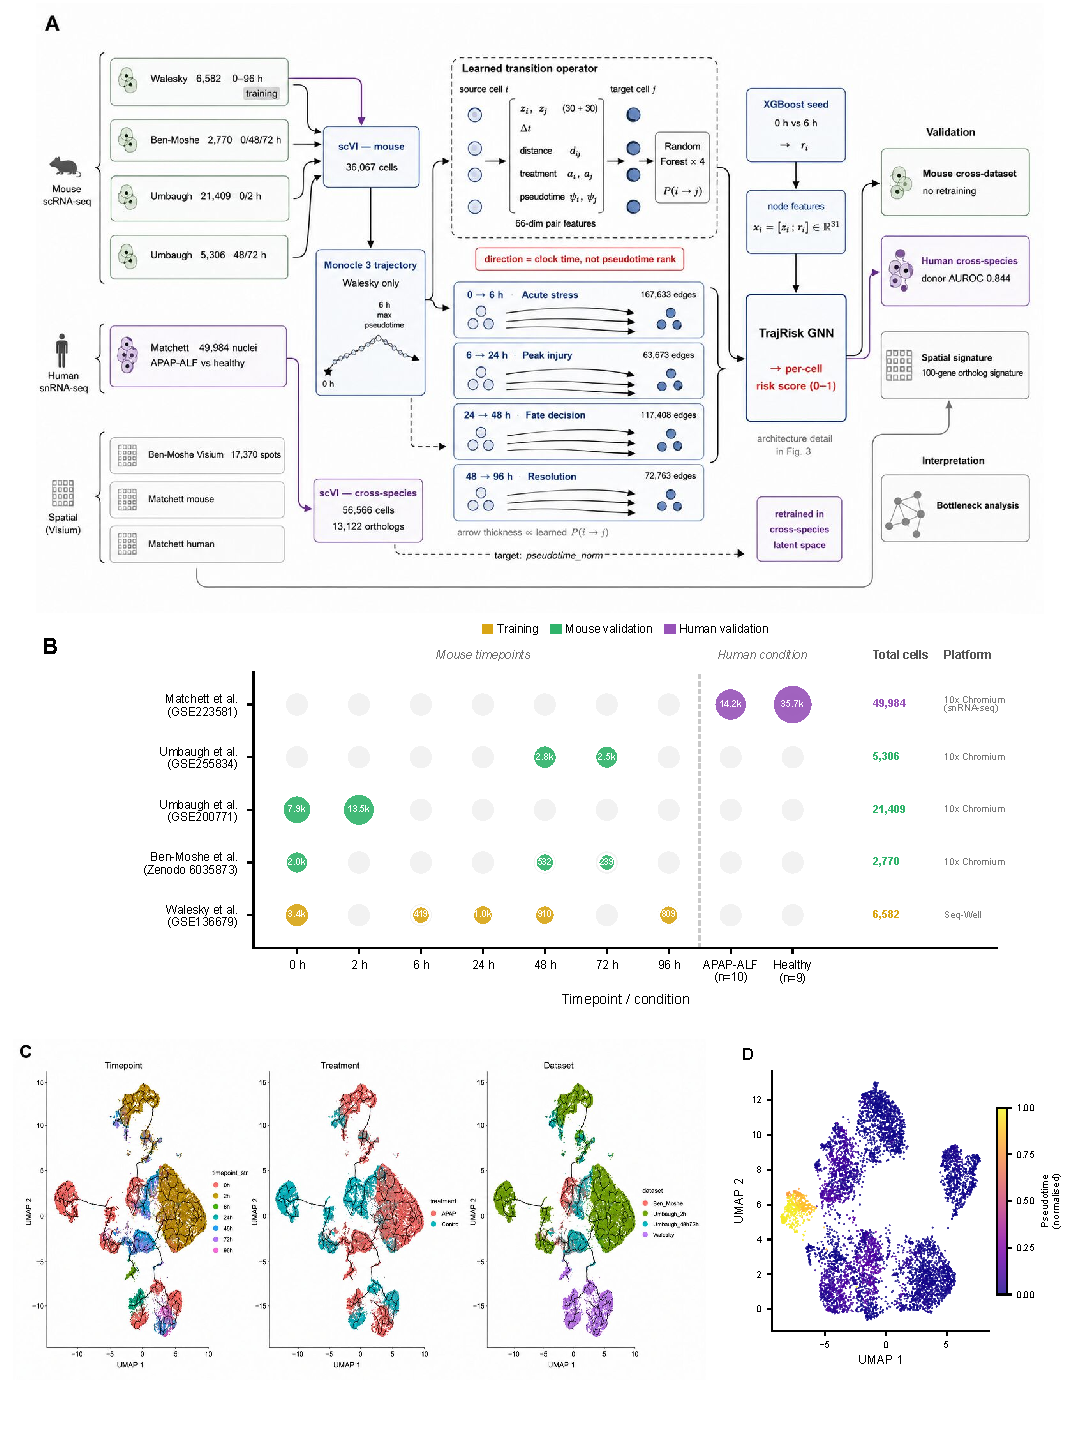
\includegraphics[width=\textwidth,trim={0.000bp 395.000bp 0.000bp 0.000bp},clip]{figures/figure_1.pdf}
\caption{\textbf{\FigOneTitle{}} \textbf{(A)} \FigOneA{}}
\label{fig:1}
\end{figure*}
\begin{figure*}[!tp]
\centering
\ContinuedFloat
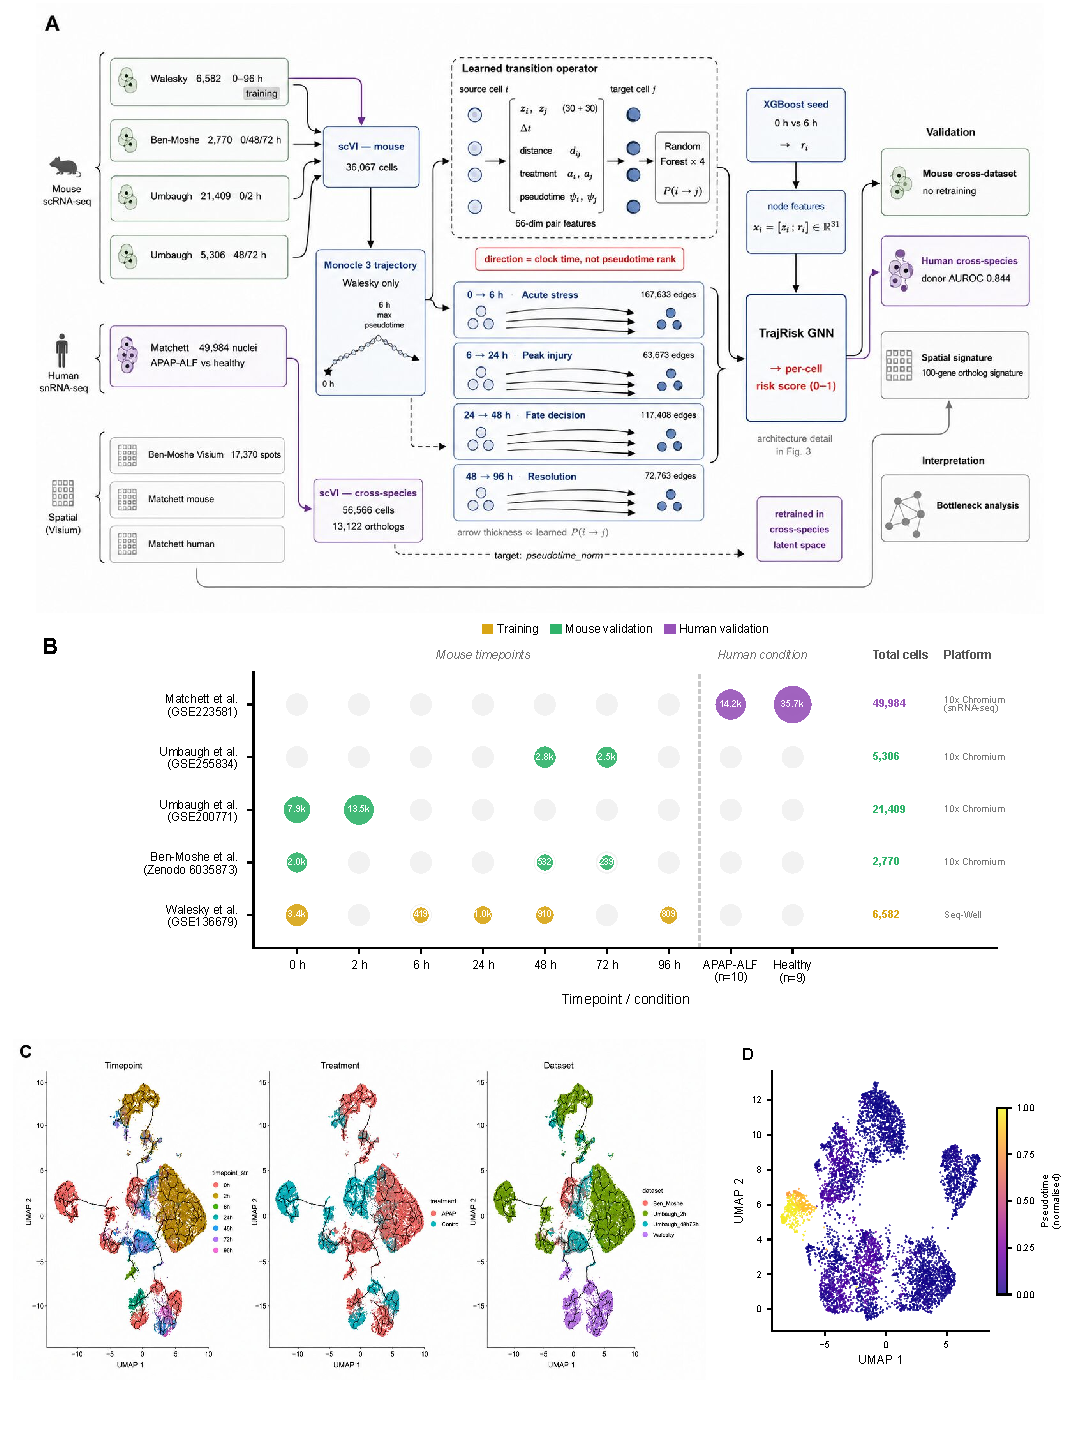
\includegraphics[width=\textwidth,trim={0.000bp 192.000bp 0.000bp 299.000bp},clip]{figures/figure_1.pdf}
\par\vspace{8pt}
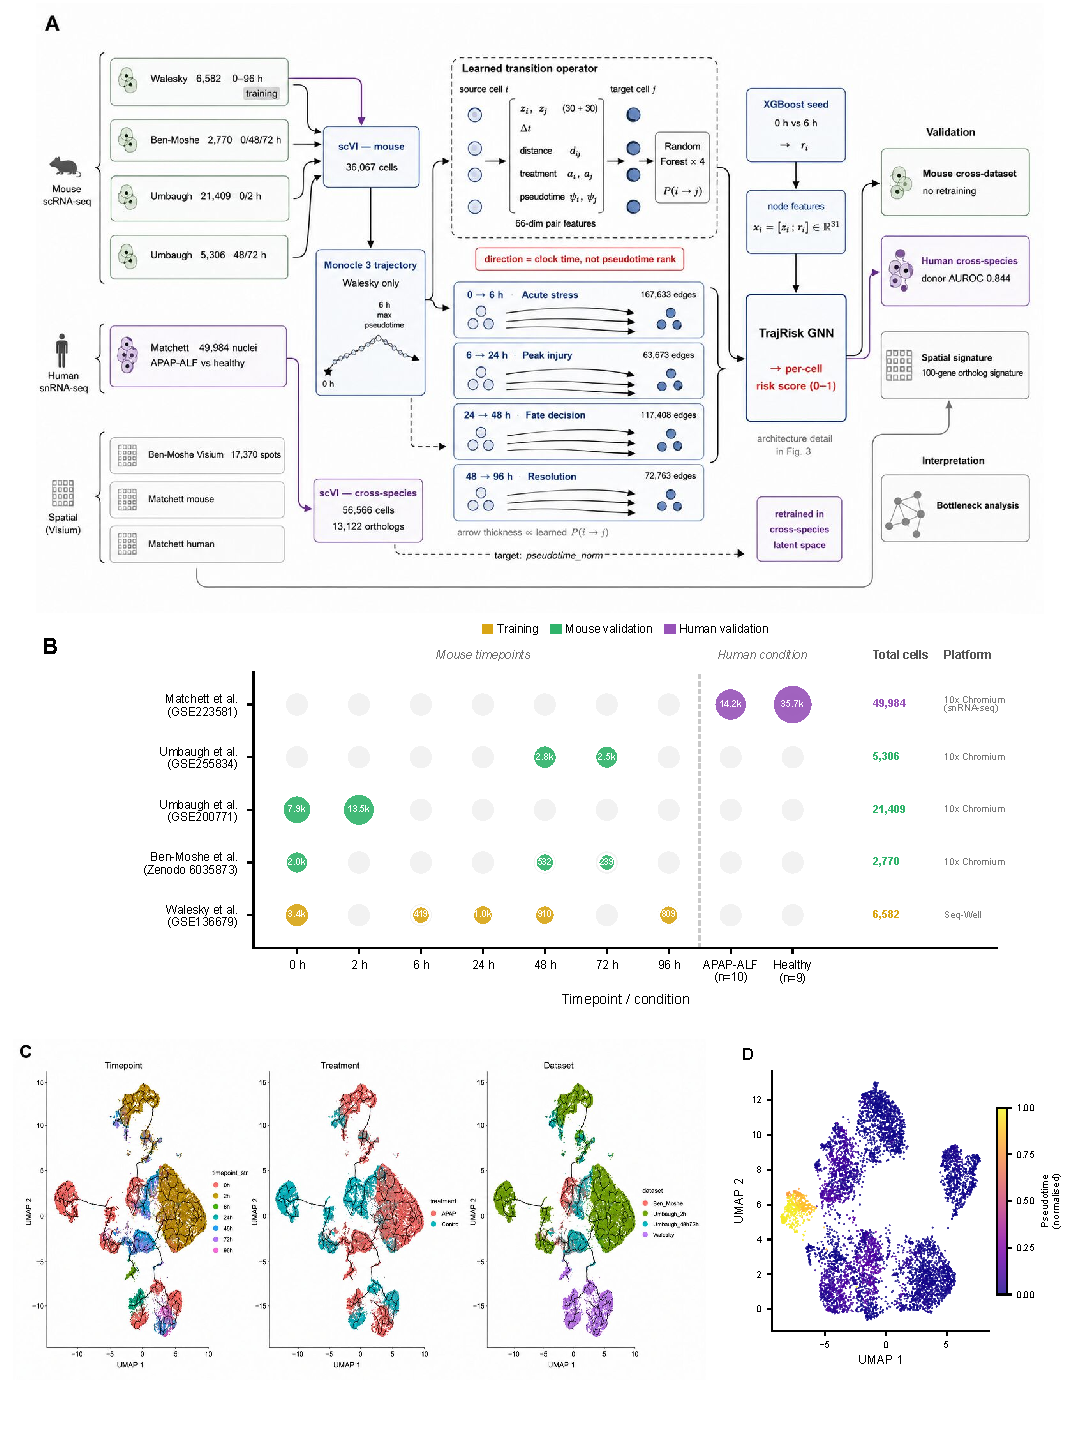
\includegraphics[width=\textwidth,trim={0.000bp 4.000bp 0.000bp 502.000bp},clip]{figures/figure_1.pdf}
\caption{\textbf{\FigOneTitle{} (continued)} \textbf{(B)} \FigOneB{} \textbf{(C)} \FigOneC{} \textbf{(D)} \FigOneD{} \FigOneNotes{}}
\end{figure*}

\subsection*{Random Forest classifiers learn directed, treatment-aware transition probabilities}

We trained one Random Forest classifier per temporal scale to predict nearest-neighbor-defined cell-pair transition labels (\hyperref[sec:methods]{Methods}). Five-fold stratified cross-validation yielded AUROC values of 0.9936 \ensuremath{\pm} 0.0002 (Scale 1, 0~h \ensuremath{\rightarrow} 6~h), 0.9871 \ensuremath{\pm} 0.0011 (Scale 2, 6~h \ensuremath{\rightarrow} 24~h), 0.9901 \ensuremath{\pm} 0.0004 (Scale 3, 24~h \ensuremath{\rightarrow} 48~h), and 0.9929 \ensuremath{\pm} 0.0009 (Scale 4, 48~h \ensuremath{\rightarrow} 96~h), with out-of-bag accuracy estimates of 0.961, 0.949, 0.955, and 0.965, respectively (\FigRef{2}{B}; \TableRef{S1}). The most important single feature across all scales was Euclidean distance in scVI latent space, consistent with the k-nearest-neighbor-based training labels. The learned transition matrices diverged substantially from a distance-only Gaussian kernel (\FigRef{2}{C}): row-wise Pearson correlations between each learned matrix and its Gaussian baseline were low (Scale 1: 0.246; Scale 2: 0.187; Scale 3: 0.249; Scale 4: 0.403), showing that the learned weights differ from a distance-only kernel. The RF classifiers also receive treatment, normalized pseudotime, and latent coordinates. Their cross-validation evaluates agreement with the constructed neighbor labels rather than independently observed biological transitions.

The resulting matrices remained numerically close to the stochasticity constraint after sparsification (row sums = 1.000, SD < 10\textsuperscript{-6}) and retained high sparsity (99.6-99.9\%). Per-cell transition entropy varied across scales (\FigRef{2}{D}; \TableRef{S1}). Scale 2 had the highest mean entropy (4.88 \ensuremath{\pm} 0.42 nats), and Scale 1 the lowest (3.81 \ensuremath{\pm} 0.26 nats); Scales 3 and 4 had intermediate means of 4.58 and 4.24 nats. These values summarize heterogeneity in outgoing transition weights, rather than the number or probability of biological fates available to a cell.

\begin{figure*}[!tp]
\centering
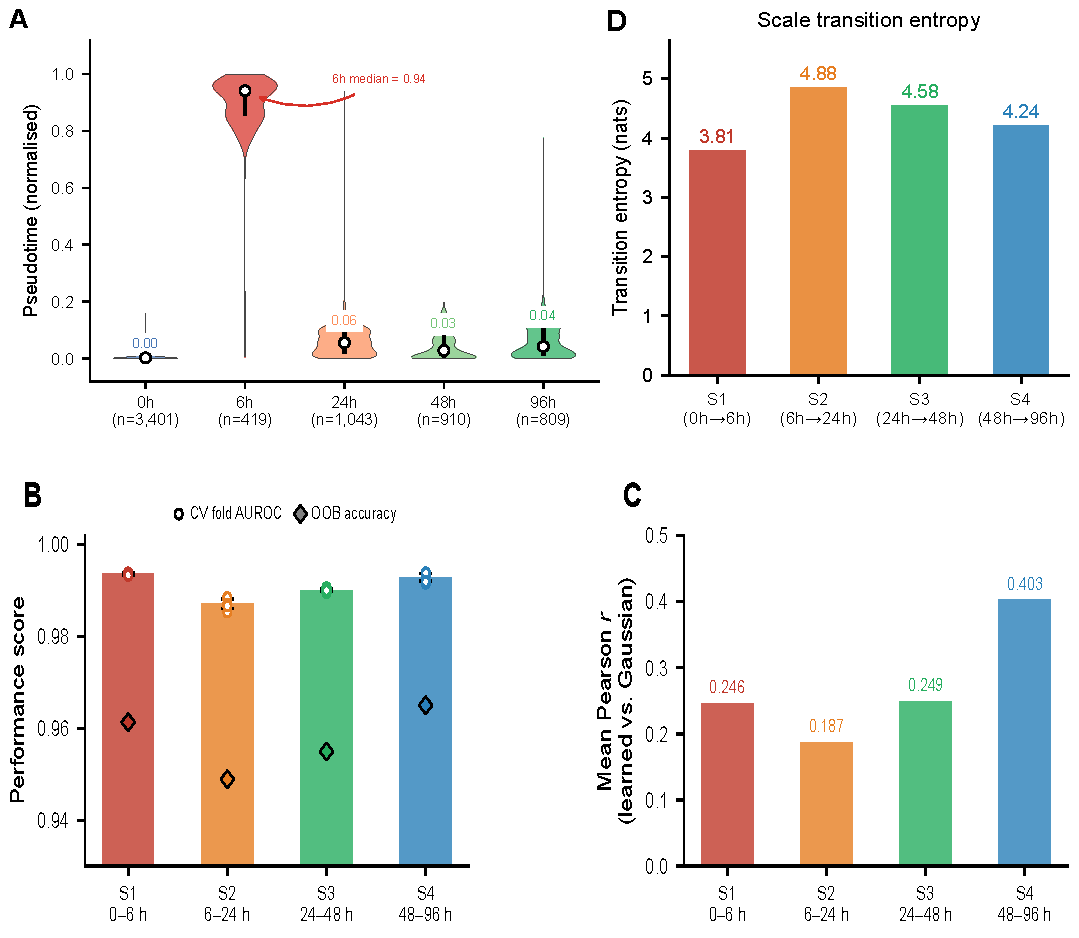
\includegraphics[width=\textwidth,trim={0.000bp 0.000bp 0.000bp 0.000bp},clip]{figures/figure_2.pdf}
\caption{\textbf{\FigTwoTitle{}} \textbf{(A)} \FigTwoA{} \textbf{(B)} \FigTwoB{} \textbf{(C)} \FigTwoC{} \textbf{(D)} \FigTwoD{} \FigTwoNotes{}}
\label{fig:2}
\end{figure*}

\subsection*{TrajRiskGNN learns biologically coherent trajectory-state representations}

The TrajRiskGNN architecture is summarized in \FigRef{3}{A}. The validation-AUROC-best checkpoint at epoch 144 was used for downstream analyses; training history and validation performance are shown in \FigRefs{3}{B--3D}. The model achieved a validation AUROC of 0.9071 (95\% CI 0.8843--0.9310), AUPRC of 0.7707, and a Spearman correlation of 0.5814 with normalized pseudotime (p = 4.65\ensuremath{\times}10\textsuperscript{-120}; \TableRef{S2A}). The train-validation Spearman gap was 0.029.

TrajRisk scores followed a pattern consistent with the reference injury trajectory (\FigRef{3}{E}). 0~h root hepatocytes had the lowest mean score (0.008; 0.0\% exceeding a predicted-score threshold of 0.10), while 6~h APAP hepatocytes, sampled during acute injury, had the highest mean score (0.917; 99.3\% exceeding threshold). Mean scores declined at 24~h (0.047, 5.2\% exceeding) and 48~h (0.030, 0.9\%), with a modest rise at 96~h (0.045, 5.6\%) consistent with a persistent compensation subpopulation. Scale-association analysis showed that Scale 1 (Acute Stress) embedding norms were positively associated with the TrajRisk score, whereas Scale 3 (Fate Decision) embedding norms were negatively associated with it (Spearman \ensuremath{\rho} = +0.325 and -0.372, respectively; \FigRef{3}{F}). A PCA of the concatenated 256-dimensional multi-scale representation, colored by sampling timepoint and by predicted TrajRisk score, is shown in \FigRefs{S2}{B and S2C}.

\begin{figure*}[!tp]
\centering
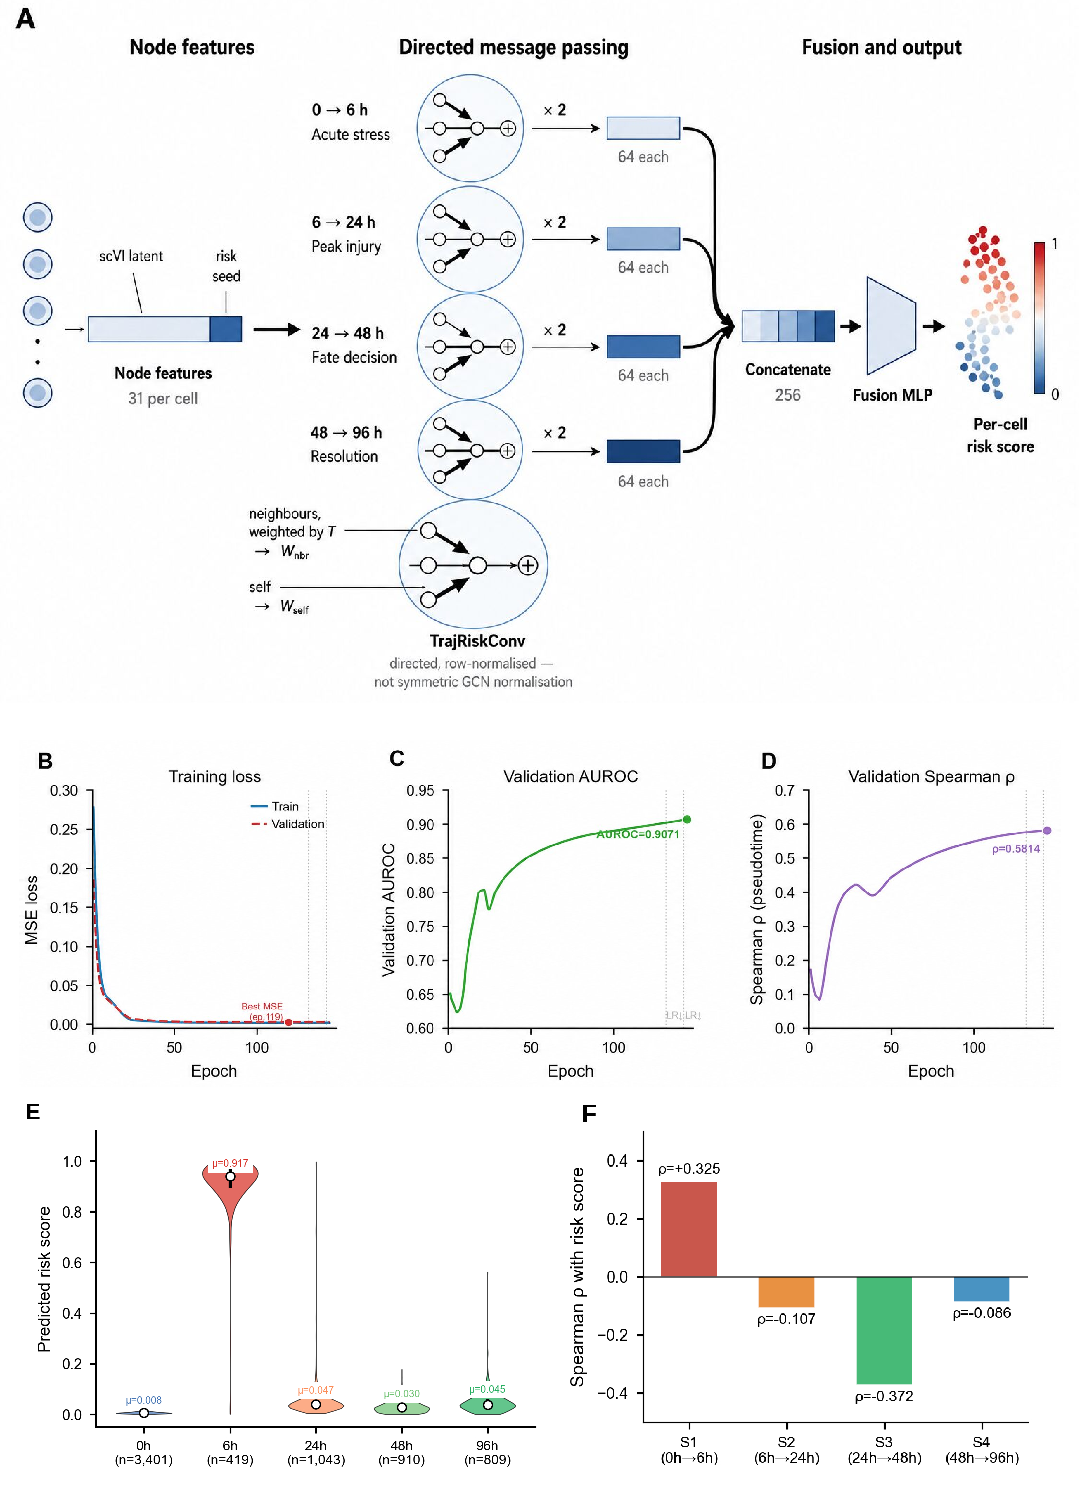
\includegraphics[width=\textwidth,trim={0.000bp 372.000bp 0.000bp 0.000bp},clip]{figures/figure_3.pdf}
\caption{\textbf{\FigThreeTitle{}} \textbf{(A)} \FigThreeA{}}
\label{fig:3}
\end{figure*}
\begin{figure*}[!tp]
\centering
\ContinuedFloat
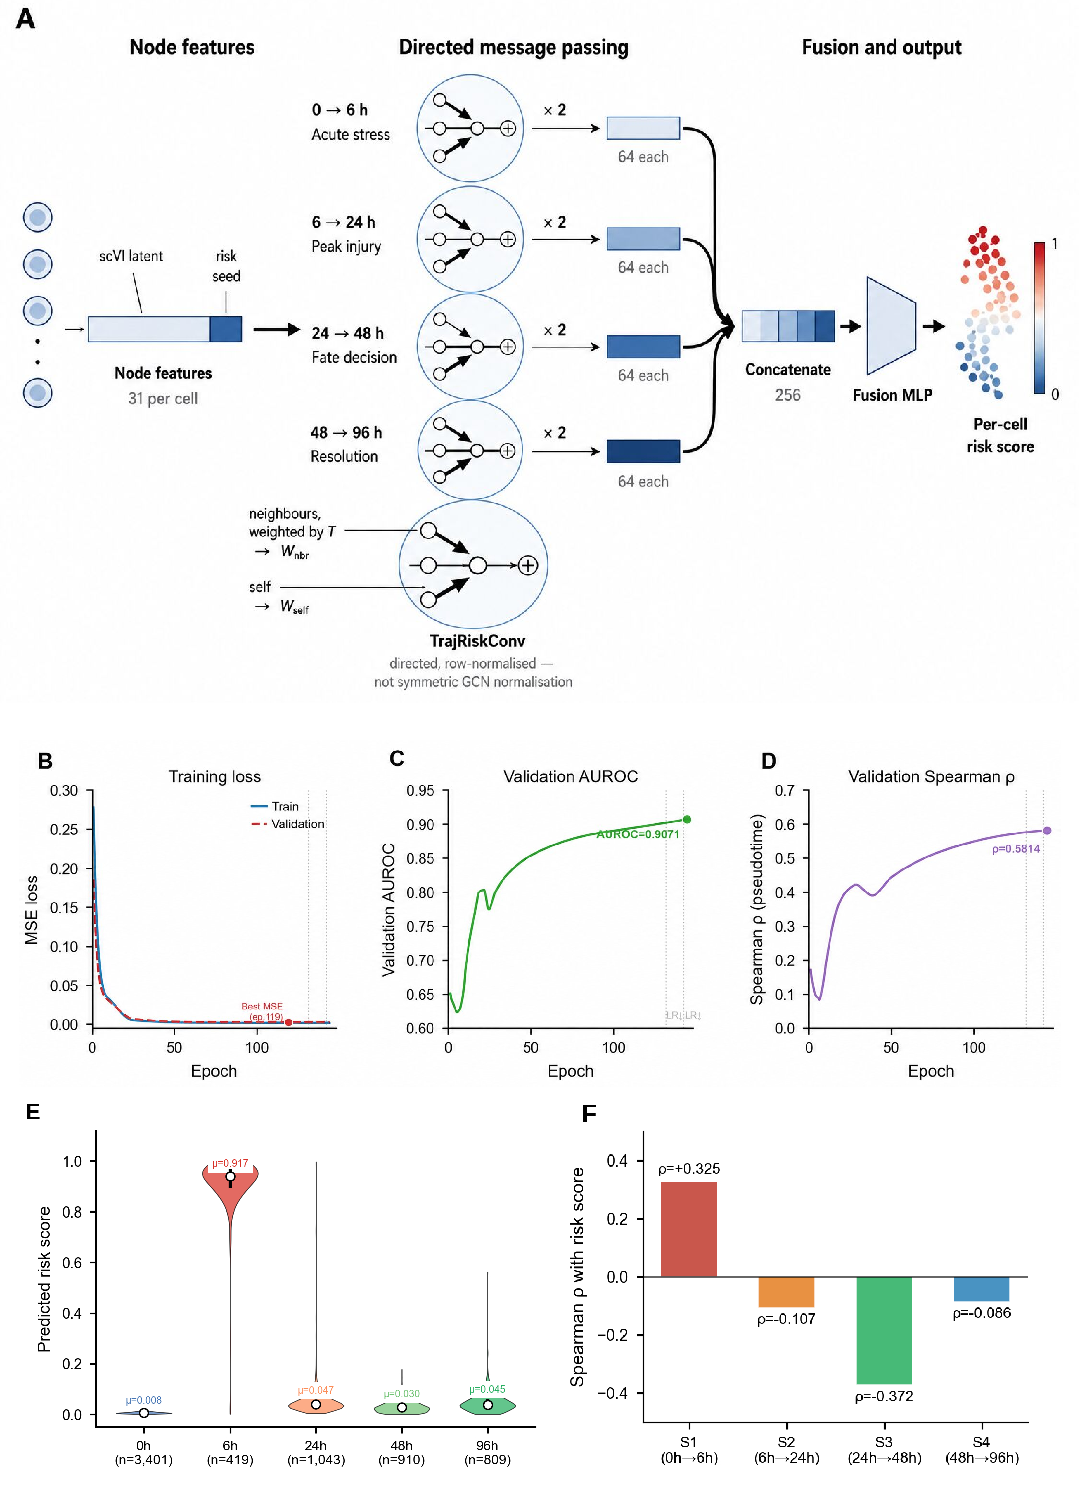
\includegraphics[width=\textwidth,trim={0.000bp 3.000bp 0.000bp 352.000bp},clip]{figures/figure_3.pdf}
\caption{\textbf{\FigThreeTitle{} (continued)} \textbf{(B)} \FigThreeB{} \textbf{(C)} \FigThreeC{} \textbf{(D)} \FigThreeD{} \textbf{(E)} \FigThreeE{} \textbf{(F)} \FigThreeF{} \FigThreeNotes{}}
\end{figure*}

\subsection*{Benchmark comparisons show timepoint-dependent performance}

We benchmarked TrajRisk against four baselines on the fixed 1,318-cell Walesky validation set (\FigRef{4}{A}; \TableRef{S2A}). Expression-only XGBoost\cite{ref048} regression (B1) achieved higher global AUROC than TrajRisk (0.9582 versus 0.9071). Both models use expression-derived features to predict expression-derived pseudotime. The TrajRisk graphs additionally incorporate reference pseudotime during construction, including for validation cells; this is a transductive within-reference evaluation rather than an independent test on unseen cells.

TrajRisk had higher global AUROC than Gaussian scalar propagation (0.856), the development-selected single-scale GNN (0.850), and expression distance from baseline controls (0.800), with one-sided paired-bootstrap p < 0.001 for each comparison (\FigRef{4}{A}). The initial XGBoost seed achieved AUROC 0.875, compared with 0.907 for TrajRisk. The seed is an acute-state classifier trained on 0~h versus 6~h cells, whereas B1 directly regresses continuous pseudotime; these are distinct expression-only comparators.

Reduced-model comparisons showed lower AUROC when learned RF transitions were replaced by Gaussian transitions (decrease of 8.1 percentage points), the seed was removed (7.9 points), one temporal scale was retained (5.7 points), or the complete GNN was replaced by scalar RF propagation (5.4 points) (\FigRefs{4}{A and 4B}; \TableRefs{S2A}{S2B}). These comparisons support sensitivity to model configuration but do not isolate every component: scalar RF propagation jointly removes nonlinear message aggregation and node-feature integration. The primary model was selected using validation AUROC, while GNN ablations used an inner development split, giving the primary model a checkpoint-selection advantage (\hyperref[sec:methods]{Methods}).

We also evaluated discrimination within recovery timepoints using average precision (AUPRC), with positive labels defined by normalized pseudotime > 0.10 (\FigRef{4}{C}; \TableRef{S2C}). After excluding 6~h cells (n = 1,234; 130 positives), TrajRisk's AUROC was 0.856, compared with 0.796 for the seed and 0.933 for B1. At 24~h (n = 209; 36 positives), TrajRisk had AUPRC 0.498 versus 0.322 for the seed and 0.379 for B1, an 11.9-percentage-point advantage over B1. B1 nevertheless had higher AUROC at each evaluated recovery timepoint. At 48~h, TrajRisk and B1 had AUPRC 0.463 and 0.597, respectively; at 96~h, the corresponding values were 0.581 and 0.692. The 96~h gain of 30.9 percentage points is relative to the seed (0.273), not B1. No formal significance tests were performed for these subset comparisons. Thus, the AUPRC advantage over B1 is confined to the 24~h subset and does not establish generally superior discrimination or future recovery outcomes.

\begin{figure*}[!tp]
\centering
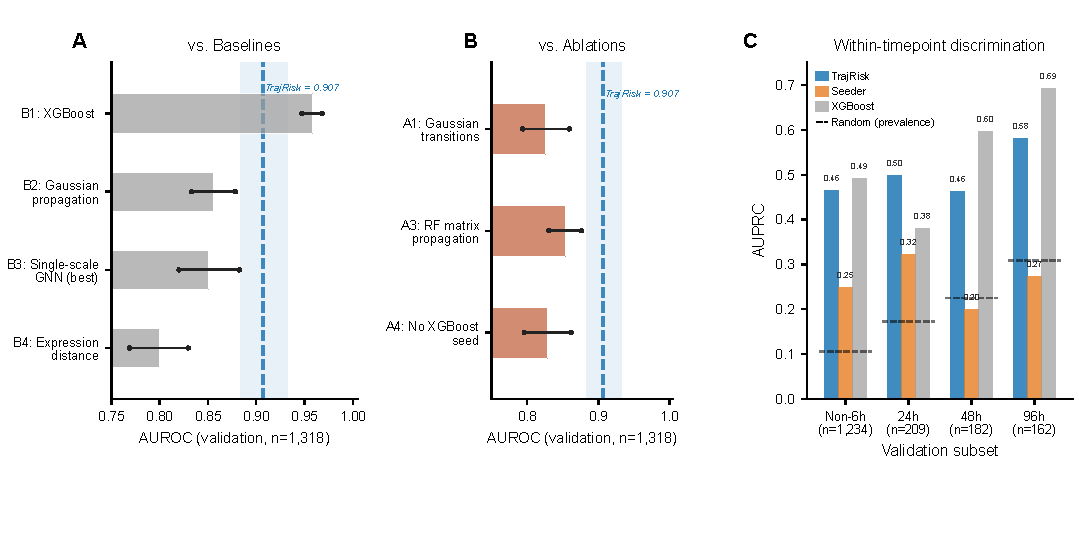
\includegraphics[width=\textwidth,trim={0.000bp 0.000bp 0.000bp 0.000bp},clip]{figures/figure_4.pdf}
\caption{\textbf{\FigFourTitle{}} \textbf{(A)} \FigFourA{} \textbf{(B)} \FigFourB{} \textbf{(C)} \FigFourC{} \FigFourNotes{}}
\label{fig:4}
\end{figure*}

\subsection*{External mouse transfer is cohort-dependent}

We evaluated three external mouse cohorts using frozen Walesky-trained models (\FigRef{5}{A}; \TableRef{S3A}). In Ben-Moshe hepatocytes (n = 2,770), APAP-versus-control AUROC was 0.7197 for Reference-KNN and 0.8069 for \SelfOnly{} TrajRisk, compared with 0.8541 for the seed and 0.8544 for B1. In the Umbaugh 48/72~h cohort (n = 5,306), the corresponding AUROCs were 0.7939, 0.8958, 0.9330, and 0.9423. Both TrajRisk variants therefore underperformed expression-only comparators on treatment discrimination in these later cohorts. Treatment status is a different endpoint from the normalized reference pseudotime used for TrajRisk training; this distinction does not by itself establish that lower transferred scores accurately identify recovery.

At Umbaugh 2~h, a sampling time absent from supervised model training (n = 21,409), Reference-KNN AUROC was 0.6524, compared with 0.6087 for \SelfOnly{}, 0.6465 for the seed, and 0.6422 for B1 (\FigRef{5}{B}; \TableRef{S3A}). Reference-KNN thus showed a small observed advantage over the expression-only comparators at early injury, with no reported pairwise significance test. External cohorts were included in the unsupervised scVI integration, so frozen-model transfer here does not represent evaluation of an entirely unseen expression distribution.

In all 5,306 Umbaugh 48/72~h hepatocytes, \SelfOnly{} scores correlated positively with \textit{Cdkn1a} expression (Spearman \ensuremath{\rho} = 0.382; p = 3.84\ensuremath{\times}10\textsuperscript{-184}; \FigRef{5}{C}; \TableRef{S3B}). Reference-KNN had \ensuremath{\rho} = 0.313, whereas the seed and B1 had stronger correlations (0.418 and 0.404). The association connects the transferred score to a p21-associated transcriptional program but does not demonstrate added information over expression-only comparators or a causal mechanism; \textit{Cdkn1a} transcript detection does not directly measure p21 protein.

\begin{figure*}[!tp]
\centering
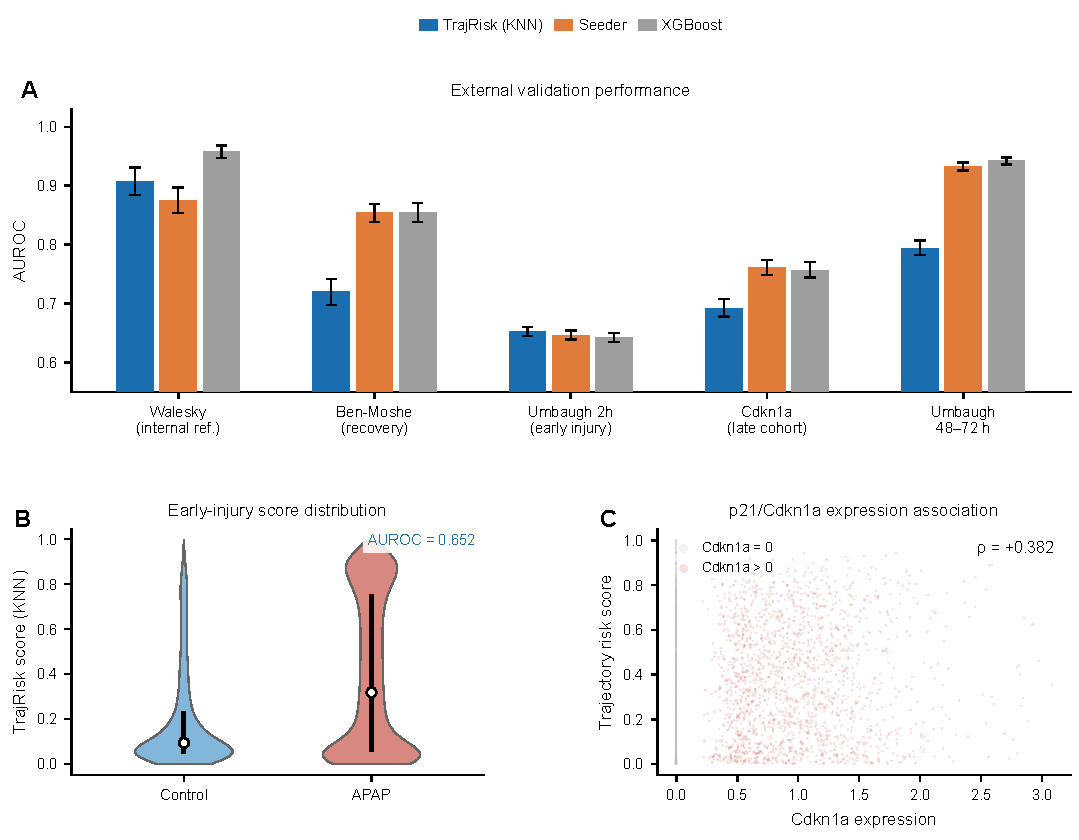
\includegraphics[width=\textwidth,trim={0.000bp 0.000bp 0.000bp 0.000bp},clip]{figures/figure_5.pdf}
\caption{\textbf{\FigFiveTitle{}} \textbf{(A)} \FigFiveA{} \textbf{(B)} \FigFiveB{} \textbf{(C)} \FigFiveC{} \FigFiveNotes{}}
\label{fig:5}
\end{figure*}

\subsection*{TrajRisk transfers the mouse trajectory-state score to human APAP-ALF donors}

Cross-species scVI integration of Walesky mouse hepatocytes and Matchett human hepatocyte nuclei used 13,122 shared mouse--human gene-symbol pairs retained by the uniqueness and expression-axis filters (\FigRef{6}{A}; \TableRef{S4A}). Quality-control characteristics of the 49,984 Matchett human hepatocyte nuclei are summarized in \FigRef{S1}{D}. Both species and condition ASW rounded to 0.0347, consistent with mixing in the joint latent space; the shared cross-species scVI space visualized by species and biological condition is shown in \FigRefs{S3}{A and S3B}. Donor-level \SelfOnly{} TrajRisk scores were higher in APAP-ALF donors (n = 10) than healthy donors (n = 9) (mean 0.2051 vs. 0.1088; Mann-Whitney p = 6.4\ensuremath{\times}10\textsuperscript{-3}; donor-level AUROC = 0.844; \FigRef{6}{B}; \TableRef{S4B}; \DataRef{S3}). Nucleus-level primary \SelfOnly{} scores across the same cross-species latent coordinates are shown in \FigRef{S3}{C}.

A Reference-KNN sensitivity analysis gave consistent results (p = 8.0\ensuremath{\times}10\textsuperscript{-3}; AUROC = 0.833; \TableRef{S4B}; \DataRef{S3}). The temporal composition of the 15 nearest Walesky reference neighbors used in this sensitivity analysis is summarized by human condition in \FigRef{S3}{D}; this panel is a reference-projection diagnostic rather than human trajectory inference. The primary \SelfOnly{} association remained significant after exclusion of low-nucleus-count donors (p = 2.5\ensuremath{\times}10\textsuperscript{-2}; AUROC = 0.815; \FigRef{6}{C}; \TableRef{S4B}; \DataRef{S4}).

The raw orthologous risk signature, defined by genes positively correlated with mouse pseudotime (\DataRef{S1}), had lower donor means in APAP-ALF than in healthy tissue (0.3585 versus 0.4380) and AUROC 0.056 in its prespecified direction (\TableRef{S4B}). Subtracting the 50-gene recovery signature gave a net-signature AUROC of 0.656, but the directional donor comparison remained non-significant (p = 0.135). The net signature therefore did not independently validate case--control discrimination. Reference-KNN TrajRisk and net-signature donor scores were correlated (Spearman \ensuremath{\rho} = 0.833; p = 9.4\ensuremath{\times}10\textsuperscript{-6}; \FigRef{6}{D}; \TableRef{S4C}; \DataRef{S3}). Because both use the same expression data and the cohort contains only 19 donors, this association describes concordant ordering rather than independent replication.

Human differential-expression overlap with mouse bottleneck-associated genes is reported below alongside the bottleneck analysis (\FigRef{6}{E}).

\begin{figure*}[!tp]
\centering
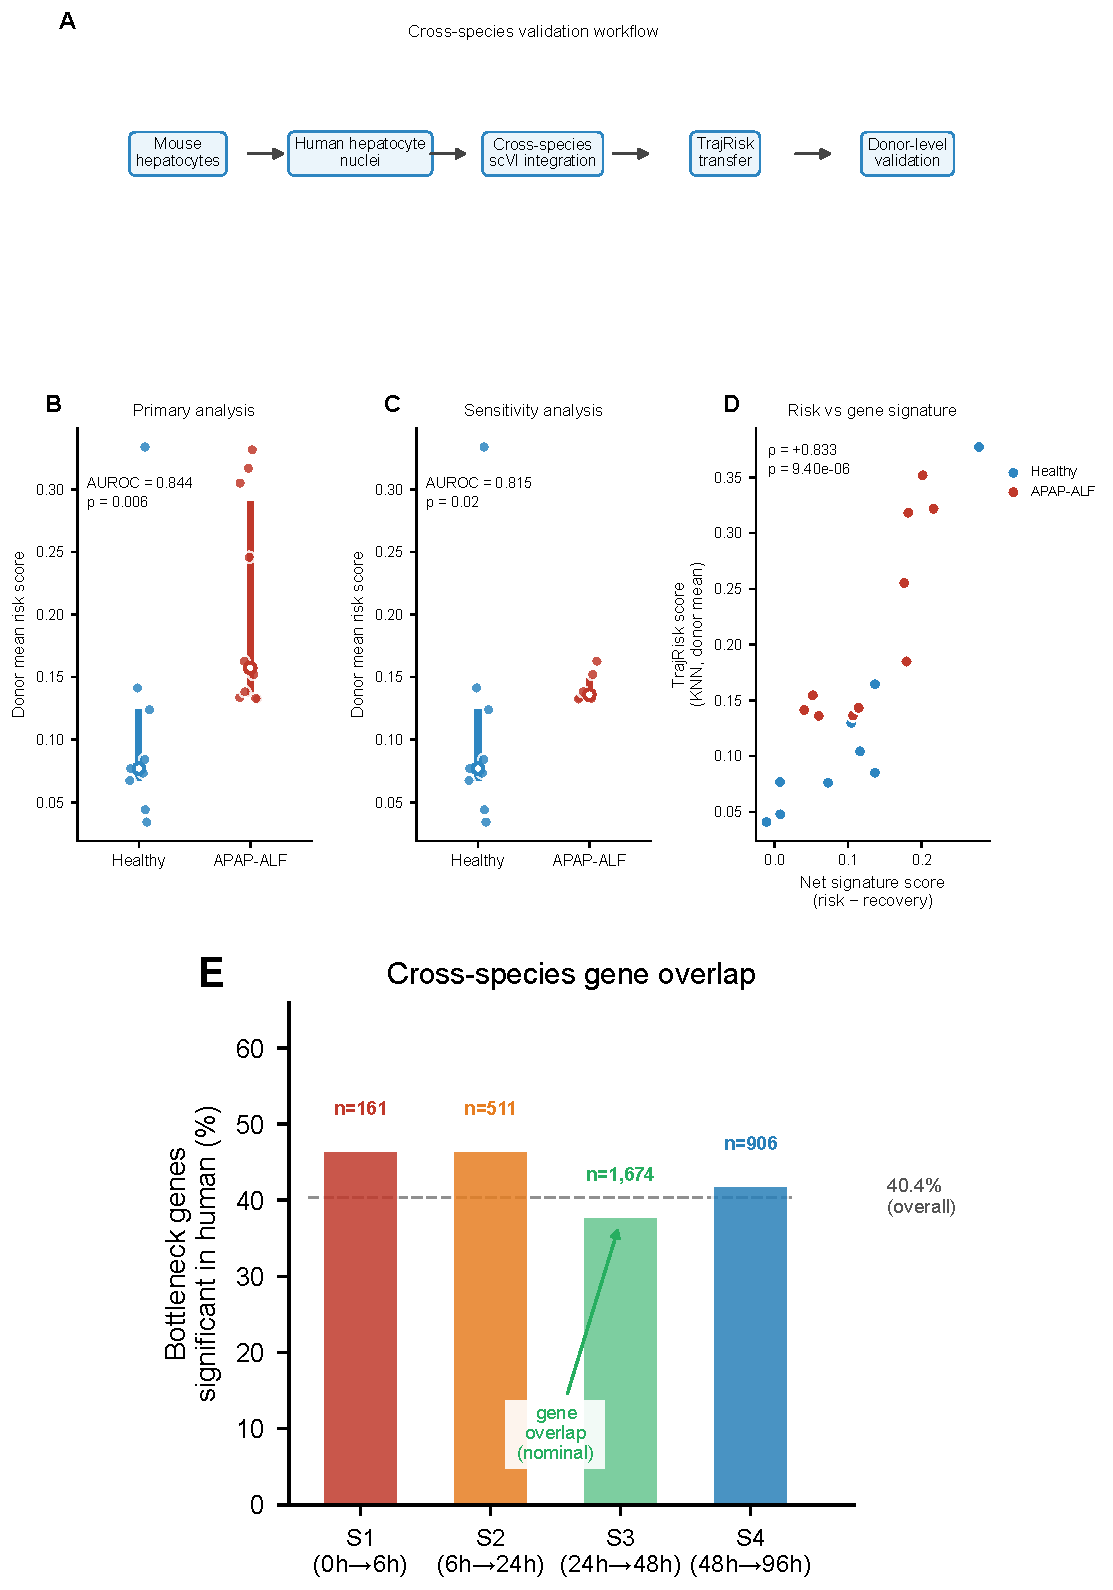
\includegraphics[width=\textwidth,trim={0.000bp 670.000bp 0.000bp 0.000bp},clip]{figures/figure_6.pdf}
\par\vspace{7pt}
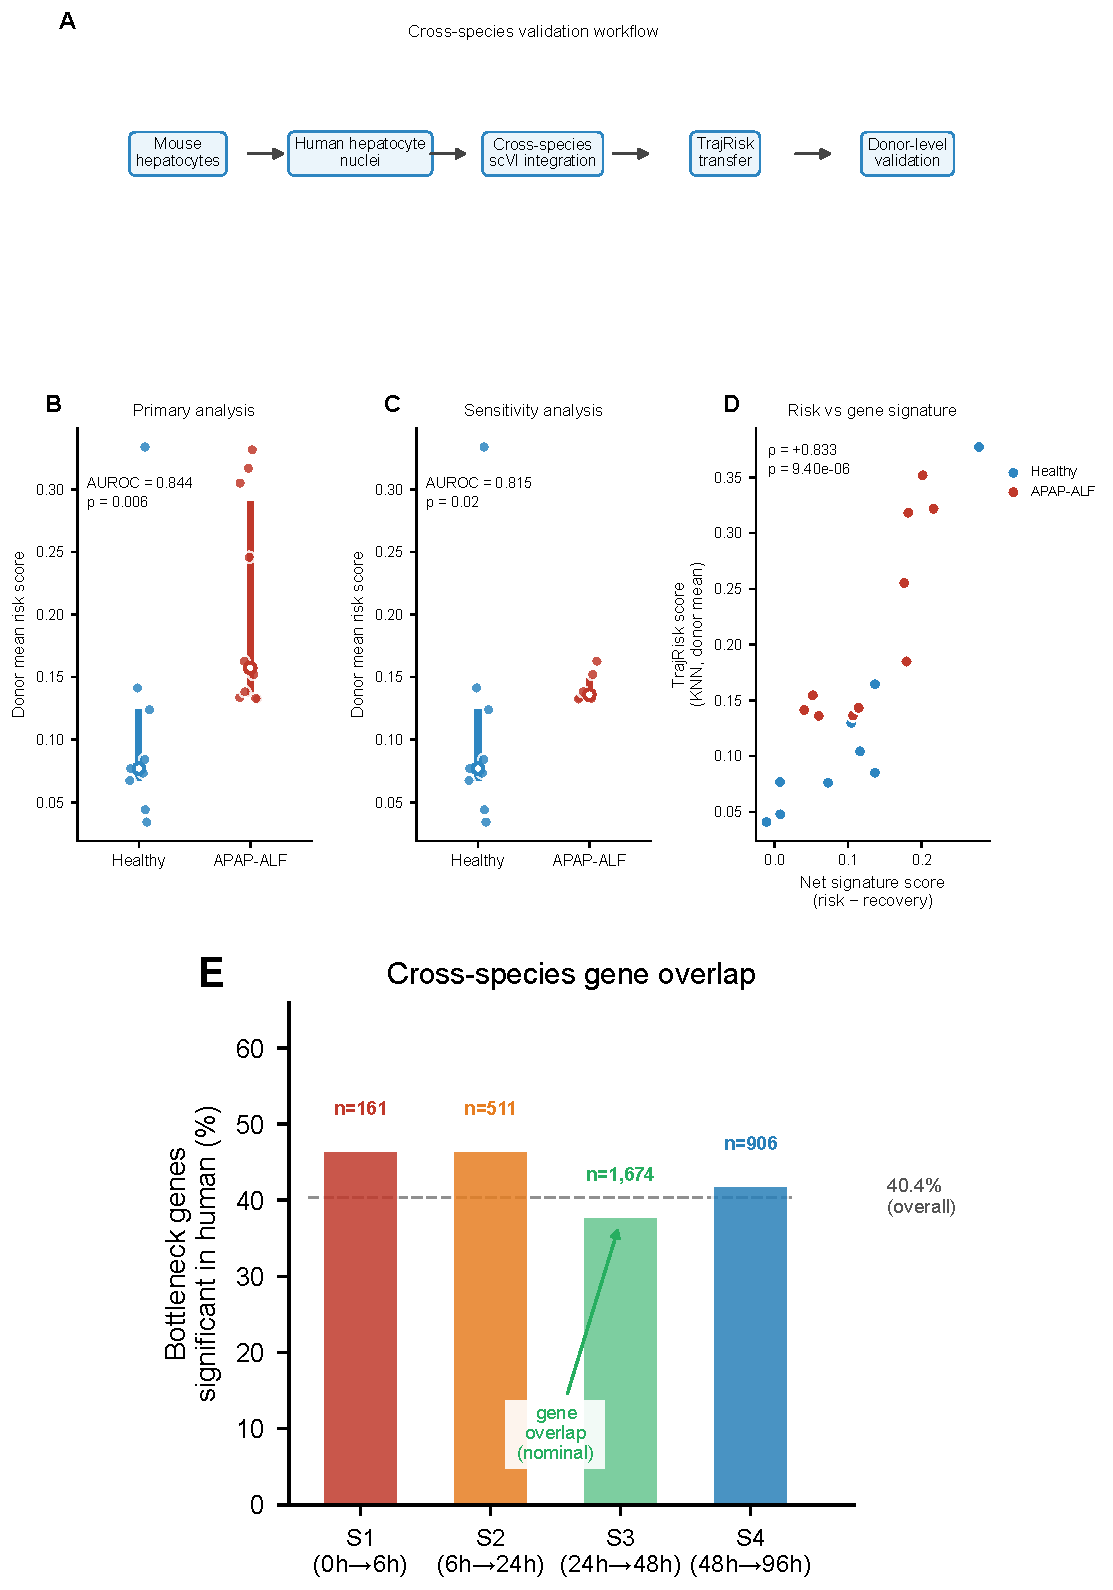
\includegraphics[width=\textwidth,trim={0.000bp 321.000bp 0.000bp 186.000bp},clip]{figures/figure_6.pdf}
\caption{\textbf{\FigSixTitle{}} \textbf{(A)} \FigSixA{} \textbf{(B)} \FigSixB{} \textbf{(C)} \FigSixC{} \textbf{(D)} \FigSixD{} \FigSixNotes{}}
\label{fig:6}
\end{figure*}
\begin{figure*}[!tp]
\centering
\ContinuedFloat
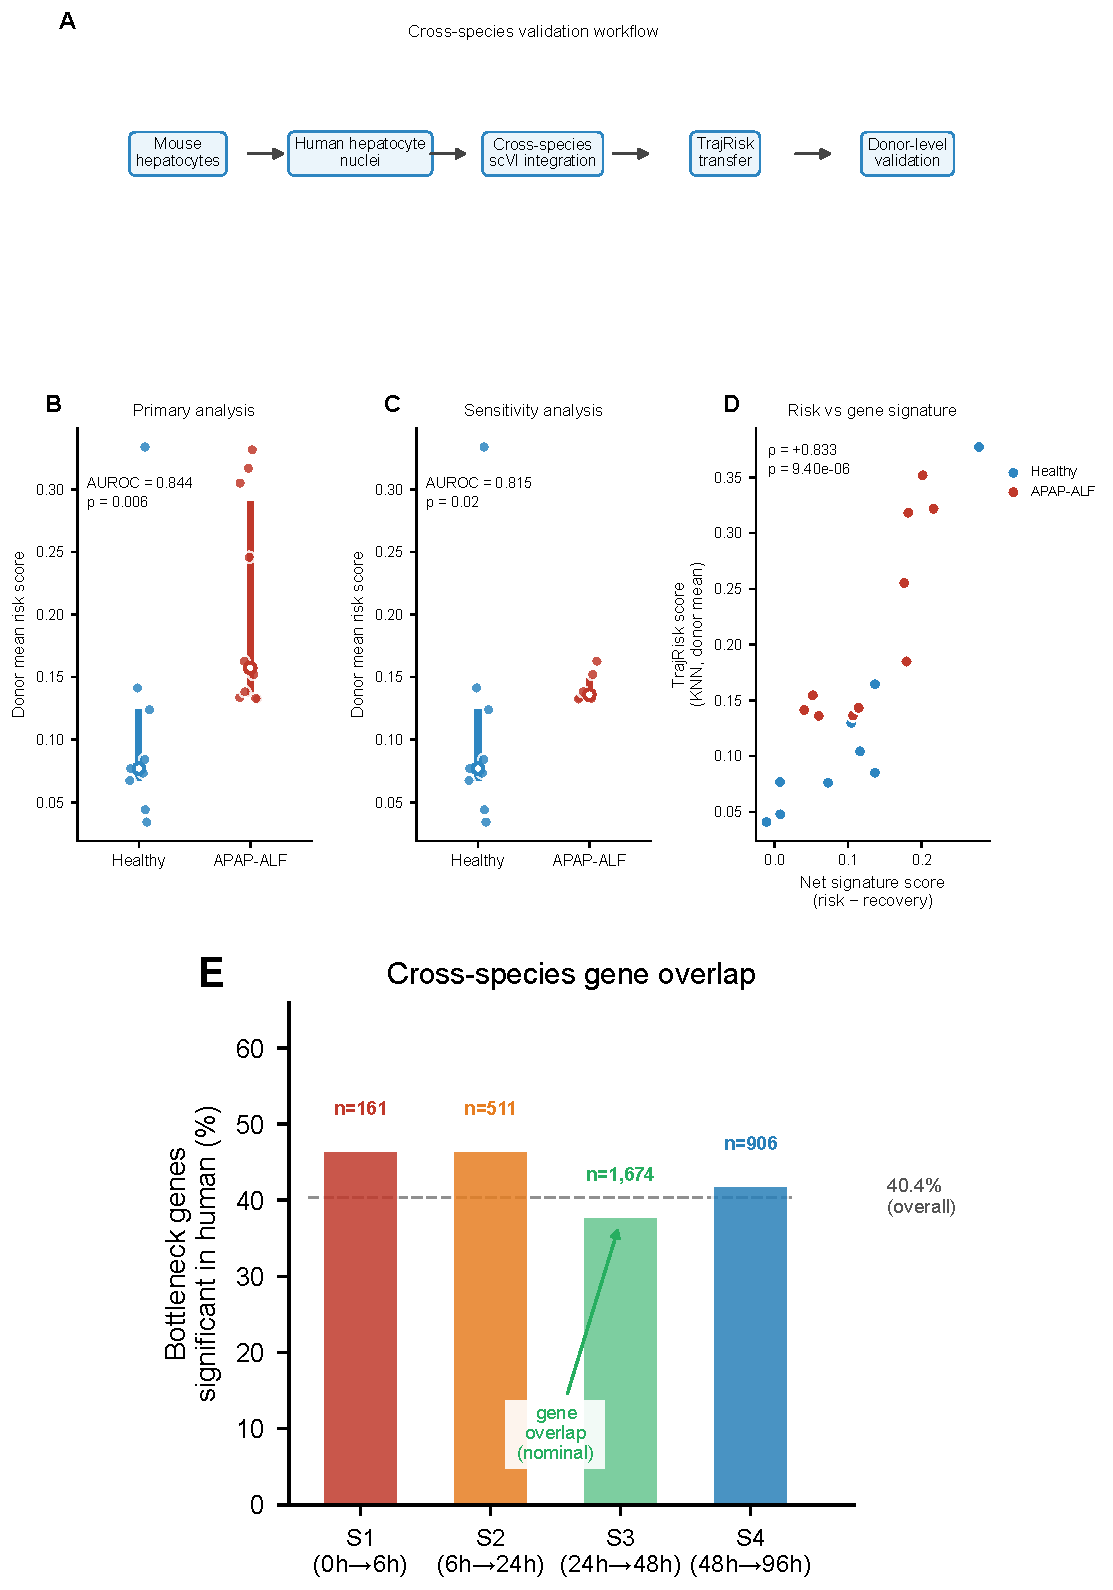
\includegraphics[width=0.79\textwidth,trim={74.000bp 0.000bp 21.000bp 447.000bp},clip]{figures/figure_6.pdf}
\caption{\textbf{\FigSixTitle{} (continued)} \textbf{(E)} \FigSixE{}}
\end{figure*}

\subsection*{Spatial localization of the orthologous risk signature varies across datasets}

We next evaluated whether the orthologous TrajRisk risk signature localized to spatial regions associated with APAP injury using two independent Visium studies (\FigRef{S4}{}). In the Ben-Moshe spatial dataset, fibrogenic spots marking the pericentral necrotic boundary were significantly enriched for the TrajRisk signature (pooled one-sided Mann--Whitney p < 10\textsuperscript{-300}); enrichment remained significant at 24~h (p = 1.55\ensuremath{\times}10\textsuperscript{-48}), 48~h (p = 9.37\ensuremath{\times}10\textsuperscript{-300}), and 72~h (p = 1.19\ensuremath{\times}10\textsuperscript{-301}), consistent with localization to regions of active injury (\FigRef{S4}{A}; \TableRef{S5A}). These exploratory tests pool spots and do not estimate significance across independent biological replicates.

By contrast, the TrajRisk \textbf{risk signature} was not enriched in anatomically defined pericentral regions of either Matchett spatial dataset. In mouse Visium sections, risk-signature scores were similar between pericentral and periportal spots (one-sided Mann--Whitney p = 0.087; \FigRef{S4}{B}; \TableRef{S5B}), whereas in human sections the pericentral-greater-than-periportal hypothesis was not supported (p = 1.000; \FigRef{S4}{D}; \TableRef{S5C}). Risk-signature scores were negatively correlated with \textit{Cyp2e1/CYP2E1} expression in both mouse (\ensuremath{\rho} = \ensuremath{-}0.427) and human (\ensuremath{\rho} = \ensuremath{-}0.168) tissue (\TableRefs{S5B}{S5C}). In contrast, after excluding \textit{Cyp2e1/CYP2E1} itself from the recovery signature to avoid circularity with zone definition, recovery-signature scores were significantly lower in pericentral than periportal regions in both mouse (p = 1.31\ensuremath{\times}10\textsuperscript{-57}; \FigRef{S4}{C}; \TableRef{S5B}) and human (p = 2.96\ensuremath{\times}10\textsuperscript{-153}; \FigRef{S4}{E}; \TableRef{S5C}) datasets. APAP-ALF human sections nevertheless showed descriptively higher mean risk-signature scores than healthy sections across pericentral, midlobular, and periportal zones (\FigRef{S4}{F}; \TableRef{S5D}; \DataRef{S5}); no zone-level case-control significance test was performed because spots within a section are not independent biological replicates.

\subsection*{Bottleneck analysis identifies scale-specific programs and a candidate recovery gateway}

Risk flux analysis across 421,477 graph edges (\hyperref[sec:methods]{Methods}) showed that Scale 2 (Peak Injury, 6~h \ensuremath{\rightarrow} 24~h) carried the largest total flux, with 98.5\% of its edges showing negative amplification as TrajRisk scores decreased from the peak. In contrast, Scale 1 (Acute Stress, 0~h \ensuremath{\rightarrow} 6~h) edges showed uniformly positive amplification. The heavy-tailed risk-flux distributions across all four scales are shown in \FigRef{7}{A} (\TableRef{S6A}). Scale 1 ablation produced the largest total change in TrajRisk scores, showing the greatest sensitivity of the frozen model to removal of that scale (\FigRef{7}{D}; \TableRef{S6B}).

Scale 3 (Fate Decision, 24~h \ensuremath{\rightarrow} 48~h) showed the highest flux concentration, with 9.8\% of total scale flux carried by the top 1\% of edges (\TableRef{S6A}). The pseudotime distribution of top-flux source cells was bimodal at Scale 3, spanning both recovery-proximal and persistent-compensation 24~h states (\FigRef{7}{B}). The 43 unique 24~h source cells feeding these high-flux edges were enriched for elevated scores and pseudotime within the 24~h population: all 43 were in the top TrajRisk-score quartile among 24~h cells, and 76.7\% were high-pseudotime. By contrast, only 18.9\% of the 380 unique 48~h target cells were high-pseudotime, below the 25.1\% expected background proportion (\FigRef{7}{C}; \TableRefs{S6C}{S6D}). The source-cell enrichment was robust to the bottleneck definition: across top 0.5\%, 1\%, 2\%, 5\%, and 10\% Scale 3 flux thresholds, the fraction of high-pseudotime source cells remained above the 25.0\% background among all 24~h cells (\FigRef{S5}{A}; \TableRef{S6E}). These connections motivate a candidate resolution-gateway hypothesis linking compensation-associated 24~h states to recovery-proximal 48~h states. Flux contains the source score by definition, so enrichment of high-score sources is partly built into the selection. Neither lineage transitions nor a causal role in recovery are established by this model-derived analysis. In a complementary perturbation analysis, mean absolute 48~h score changes remained small across source-cell pseudotime quartiles (0.0015--0.0018), whereas the Q4 high-pseudotime group produced the largest maximum single-cell change (0.0979); all 96~h mean and maximum effects were zero (\FigRef{S5}{B}; \TableRef{S6F}).

Pathway analysis showed scale-specific programs: Scale 1 bottleneck targets were enriched for oxidative phosphorylation; Scale 2 targets showed lower expression of CYP-associated metabolic programs; Scale 3 targets showed downregulation of ribosome biogenesis, mitochondrial translation, and immediate-early stress-response programs; and Scale 4 targets showed enrichment of periportal-associated programs (\FigRef{7}{F}). Scale 3 bottleneck edges also showed significantly larger embedding shifts than background edges (p < 10\textsuperscript{-172}; \FigRef{7}{E}; \TableRef{S6G}), consistent with Scale 3 being a representational as well as a flux bottleneck.

We separately assessed human differential-expression overlap with mouse bottleneck-associated programs. Among 2,549 tested mouse-gene mappings, 1,036 (40.6\%) met the nominal human differential-expression criterion in APAP-ALF versus healthy donors (p \ensuremath{\leq} 0.05; \DataRef{S2}). These records correspond to 1,023 significant human genes among 2,534 distinct human genes tested (40.4\%). The corresponding distinct-human-gene overlap was 46.6\%, 46.6\%, 37.8\%, and 41.9\% for Scales 1--4, respectively (\FigRef{6}{E}). The criterion requires nominal significance in human donors, but not agreement in fold-change direction between species. These overlaps are exploratory, unadjusted for multiple testing, and not benchmarked against a matched gene background; cross-sectional human sampling also does not reproduce the temporally defined mouse transitions.

\begin{figure*}[!tp]
\centering
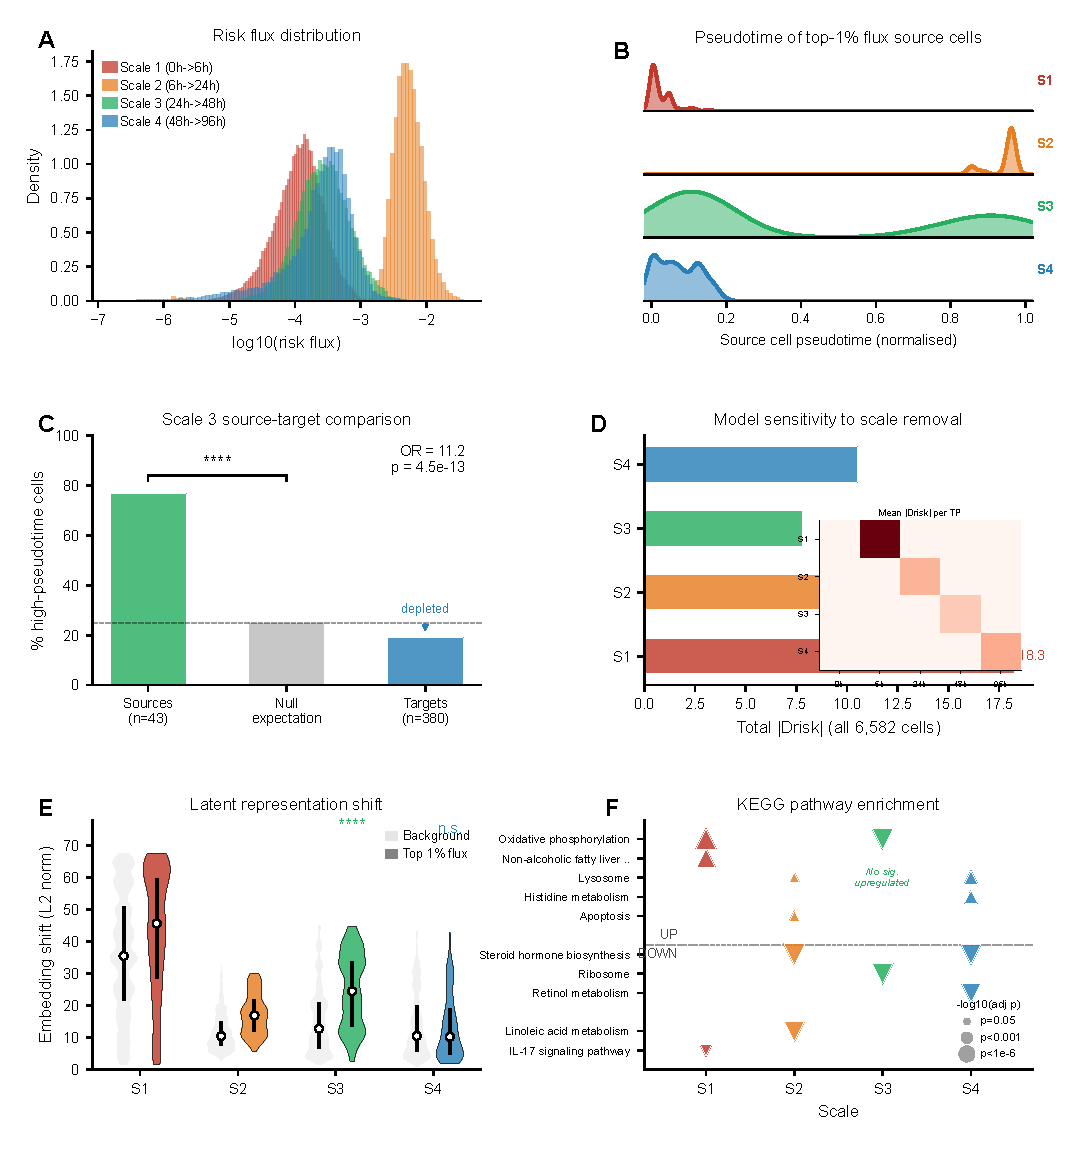
\includegraphics[width=\textwidth,trim={0.000bp 197.000bp 0.000bp 0.000bp},clip]{figures/figure_7.pdf}
\caption{\textbf{\FigSevenTitle{}} \textbf{(A)} \FigSevenA{} \textbf{(B)} \FigSevenB{} \textbf{(C)} \FigSevenC{} \textbf{(D)} \FigSevenD{} \FigSevenNotes{}}
\label{fig:7}
\end{figure*}
\begin{figure*}[!tp]
\centering
\ContinuedFloat
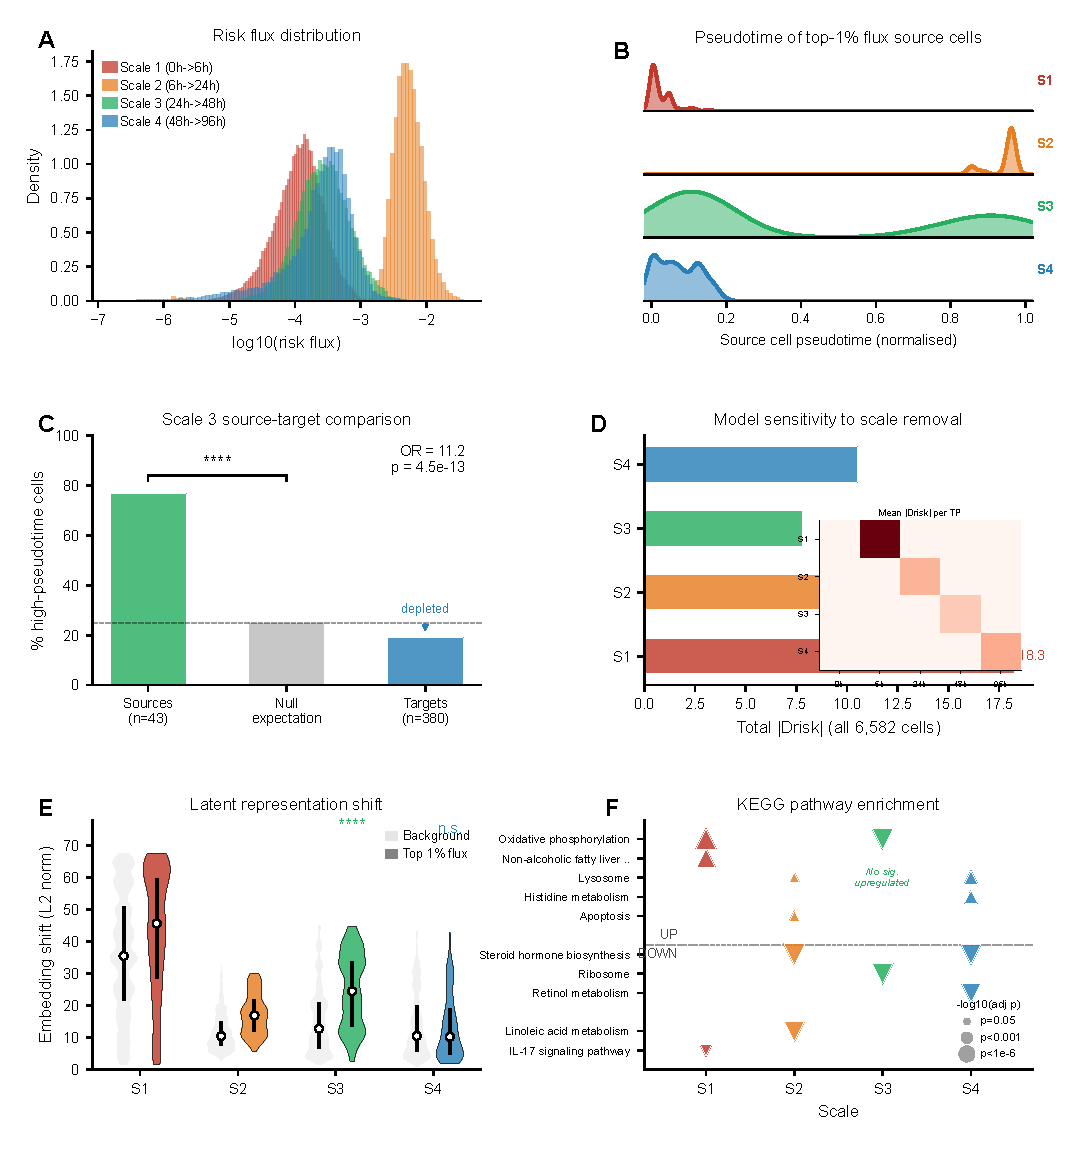
\includegraphics[width=\textwidth,trim={0.000bp 0.000bp 0.000bp 372.000bp},clip]{figures/figure_7.pdf}
\caption{\textbf{\FigSevenTitle{} (continued)} \textbf{(E)} \FigSevenE{} \textbf{(F)} \FigSevenF{}}
\end{figure*}


% Converted from the reference-locked manuscript.
% Final interpretation pass; operational score and inference limits follow the locked Methods.
\section*{Discussion}

TrajRisk integrates treatment-aware RF transition probabilities with a multi-scale GNN to represent hepatocyte states during APAP-induced liver injury. Four temporally defined graphs reflect the succession of metabolic and oxidative stress, injury-associated inflammation, and regenerative or recovery programs described in APAP studies.\cite{ref010,ref018,ref034,ref049} The benefit over expression-only XGBoost was localized: TrajRisk had higher average precision at 24~h, whereas XGBoost had higher global AUROC, higher AUROC at every evaluated recovery timepoint, and higher average precision at 48~h and 96~h. The 96~h advantage was over the acute-state seed, not the pseudotime-regression baseline. Reporting both aggregate and subgroup performance exposes differences that a single discrimination metric can obscure.\cite{ref050,ref051} Reduced-model comparisons support sensitivity to the temporal graphs, seed, and feature integration, but joint changes in some ablations and unequal checkpoint-selection protocols preclude assigning an independent contribution to every component. The framework's contribution is therefore a temporally structured representation and a way to examine transition-associated programs, rather than uniformly superior discrimination.

Directed transition graphs complement methods that obtain directional information from RNA velocity\cite{ref014,ref015} or clonal lineage tracing.\cite{ref016,ref052,ref053,ref054} Lineage-based inference can itself be affected by heterogeneous proliferation across a time course.\cite{ref055} TrajRisk uses an experimental sampling axis and treatment annotations, alongside learned cell-pair weights, in relation to methods that represent transition structure using velocity or learned embeddings.\cite{ref041,ref056,ref057} Two integrated datasets lacked the paired spliced and unspliced count layers required for velocity estimation.\cite{ref014,ref058} The sampling-time constraint provides a forward orientation even when later APAP-treated cells resemble untreated hepatocytes, as can occur during heterogeneous recovery.\cite{ref010} However, nearest-neighbor-derived pair labels are a modeling surrogate, not observed cell ancestry or independently validated transition probabilities. Integrating an acute-state classifier seed with expression features follows message-passing approaches used in single-cell and regulatory-network models.\cite{ref059,ref060} The present multi-scale model outperformed the development-selected single-scale comparator; that comparison does not establish superiority over every possible graph spanning the full trajectory.

Scale 3 (24--48~h) had the highest concentration of model-derived flux, while Scale 2 carried the largest total flux. Top-flux Scale 3 edges connected a small set of compensation-associated 24~h sources to predominantly lower-pseudotime 48~h targets. Persistent compensation has been described in the APAP model,\cite{ref010} and severe overdose can produce persistent p21-positive perinecrotic hepatocytes associated with impaired recovery.\cite{ref061} The concentration of flux motivates comparison with restricted transition states or bottlenecks in other dynamic systems.\cite{ref062,ref063} It supports a hypothesis-generating resolution gateway for follow-up experiments, rather than an established route followed by individual hepatocytes. Flux is the product of edge weight and source score; high-score-source enrichment is therefore partly inherent in the selection. Larger frozen-model perturbation effects at Scale 1 describe dependence of the network's predictions on that graph, not a ranking of biological necessity. Lineage tracing and interventions directed at candidate cell states or programs would be needed to test a role in recovery.

The primary human donor AUROC of 0.844 supports transfer of a mouse-trained trajectory-state score to APAP-ALF versus healthy donor discrimination in this cohort. Human nuclei contributed to unsupervised cross-species integration, but their condition labels were not used to train the seeder or GNN. No human pseudotime or trajectory was inferred. The primary self-only model transfers features, whereas the Reference-KNN sensitivity analysis also receives Gaussian-weighted messages from nearby mouse reference cells. This relates to reference mapping by transfer learning,\cite{ref064} hierarchical cell-type annotation,\cite{ref065} and cross-species alignment through shared or learned homology.\cite{ref066,ref067} Cross-species single-nucleus studies similarly distinguish shared disease programs from species-specific responses,\cite{ref068,ref069} including projection of human disease tissue onto mouse references.\cite{ref067} In our data, Reference-KNN scores and net-signature scores correlated across donors, but the signature's non-significant case--control result limits its value as a separate validation arm. Both scores share expression data, so concordance is an internal association. Using unweighted donor summaries rather than treating nuclei as biological replicates follows recommendations for avoiding pseudoreplication in single-cell comparisons.\cite{ref070,ref071,ref072}

The raw risk signature was higher in healthy donors and had AUROC 0.056 in the prespecified APAP-ALF-positive direction. Subtracting the recovery signature changed the donor ordering, but the net-signature comparison remained non-significant (p = 0.135; AUROC = 0.656) and was also non-significant in the low-nucleus-count sensitivity analysis. This result cannot be presented as a rescued or independent human validation. Mouse risk-signature genes include mature hepatocyte identity and metabolic genes such as \textit{Mat1a} and \textit{Hnf4a}. HNF4\ensuremath{\alpha}-associated function can decline during acute injury,\cite{ref073} and the MAT1A/S-adenosylmethionine axis is altered in liver disease.\cite{ref074} Injury-associated dedifferentiation\cite{ref073,ref075} and inflammatory reprogramming\cite{ref073,ref076} offer possible explanations for discordant signature direction between the mouse reference and human explants. These mechanisms were not tested here, and they do not establish why the aggregate signature reversed or exclude an imperfect cross-species mapping.

Spatial analyses test the localization of the mouse-derived gene signature, rather than spatially projected TrajRisk predictions; no cell-to-spot deconvolution was performed. Enrichment in Ben-Moshe fibrogenic injury-boundary spots is consistent with the original study's pericentral regenerative niche and extracellular-matrix induction.\cite{ref011} The risk signature was not enriched in \textit{Cyp2e1}/\textit{CYP2E1}-defined pericentral zones in either Matchett dataset. Constitutive metabolic zonation\cite{ref077,ref078,ref079} and injury-boundary annotation describe different tissue properties. Cell loss, repair-associated remodeling, and differing sampling windows\cite{ref011,ref080,ref081} could also contribute to these contrasting findings, but the present analyses do not distinguish among those explanations. Accordingly, the spatial evidence is dataset-dependent and does not establish a general pericentral risk signature. Spot-pooled p values describe differences within the profiled tissue and do not substitute for inference across independent animals or donors. Earlier spatial sampling and donor-resolved analyses could test whether the signature tracks transient injury-associated states.

Human nominal differential-expression overlap with mouse bottleneck-associated genes was 46.6\%, 46.6\%, 37.8\%, and 41.9\% across Scales 1--4. The overall 40.4\% counts distinct human symbols, rather than mapping records or an average of scale percentages. This criterion does not require matching fold-change direction between species and uses unadjusted human p values; it should therefore be interpreted as descriptive DE overlap rather than mechanistic conservation. Mouse and human responses can share some transcriptional programs while diverging elsewhere.\cite{ref082,ref083,ref084} A temporal mismatch is also plausible: experimental APAP studies resolve controlled exposure and recovery windows,\cite{ref085,ref086} whereas the human cohort comprises liver explants obtained at transplantation.\cite{ref019} The analysis cannot attribute the lower Scale 3 overlap to that mismatch, and no matched-background test establishes that any overlap exceeds chance. Donor discrimination, gene-level DE overlap, and conservation of a recovery mechanism remain separate questions.

Application beyond APAP hepatotoxicity remains to be tested. The core strategy of learning directed, condition-aware transition probabilities over discrete timepoints, decomposing a trajectory into biologically scoped temporal windows, and integrating an expression-based classifier seed with a graph neural network does not intrinsically depend on liver biology, and it is in principle applicable to other perturbation-response systems with comparable structure, namely multiple sampled timepoints, a treatment-versus-control contrast usable for initial seeding, and enough cells per transition to learn transition structure. Experimental designs of this kind are now common across longitudinal single-cell studies of perturbation, injury, and directed differentiation, including pooled genetic perturbation screens that couple defined perturbations to transcriptomic readouts,\cite{ref087} dense single-cell time courses of an acute cellular stress response,\cite{ref088} and staged multimodal atlases of directed organoid development,\cite{ref089} and harmonized perturbation-response datasets now aggregate many such experiments into common frameworks.\cite{ref090} Graph-based neural-network approaches have likewise been applied across a range of distinct single-cell problems, from cell-state modelling and imputation to gene-regulatory-network inference and prediction of unseen perturbation responses,\cite{ref024,ref091,ref092,ref093,ref094,ref095,ref096,ref097} which motivates evaluation of graph-based representations in new biological settings. Two aspects of the current implementation, however, are specific to this system and would need to be redefined elsewhere. The four temporal scales were chosen from established APAP injury and recovery biology,\cite{ref006,ref010,ref034} in which acute injury, functional compensation, recovery with fate divergence, and later resolution occur as temporally distinct phases, rather than learned automatically. The initial classifier seed also relies on a clear pair of phenotypically distinct reference states, here 0~h and 6~h, from which to initialise the seed. Automatic scale selection and seeding strategies for systems with multiple perturbations, branches, or phenotypic endpoints are natural directions for extending the framework beyond single-treatment, single-organ time courses.

\subsubsection*{Limitations of the study}

TrajRisk is trained to estimate normalized mouse pseudotime. Its within-mouse binary benchmark distinguishes cells above a pseudotime threshold, while external treatment and donor comparisons evaluate observed conditions. These analyses do not establish calibrated probabilities of subsequent injury, failure to recover, or clinical outcome; prospective outcome or lineage measurements would be needed to test such predictions.

Within-reference evaluation is transductive: training and validation cells share preconstructed graphs, and both cells' pseudotime values enter transition-pair features. The loss excludes validation cells, but target information has already influenced their graph connections. Shared expression-derived targets also limit the independence of all internal comparators. Selection of the primary checkpoint on validation AUROC further favors it over development-selected GNN ablations. Cell-level bootstrap intervals quantify resampling variability within these cohorts, rather than replication across studies or animals; within-timepoint and external pairwise improvements were not formally tested. RF pair-level cross-validation measures agreement with constructed neighbor labels, and pairs sharing cells are not independent biological transitions.

External performance varied by cohort. Reference-KNN showed only a small observed early-injury advantage and lower treatment discrimination than expression-only comparators in both later cohorts. Stronger seed and B1 correlations with \textit{Cdkn1a} similarly prevent interpreting its association as incremental benefit from TrajRisk. Because external cells contribute to joint unsupervised integration, these analyses do not test a fully frozen embedding on a new study. Prospective transfer with an independently fitted reference and additional cohorts would be needed to establish broader generalization.

Reference edges connecting external mouse cells or human nuclei to their nearest Walesky anchor cells were weighted by Gaussian similarity in scVI space rather than by the learned Random Forest transition probabilities used elsewhere in the model, because the Random Forest feature vector requires the target cell's normalized pseudotime, which is undefined for cells outside the primary trajectory. Mapping query cells onto a reference through latent-space similarity and nearest-neighbour matching is a well-established strategy in single-cell analysis.\cite{ref064,ref098,ref099} However, this means the Reference-KNN variant does not retain the learned, treatment-aware transition structure that distinguishes TrajRisk within the primary trajectory, and pseudotime imputation or joint transition inference for external cells could close this gap.

The human validation combines single-nucleus RNA-seq with mouse single-cell RNA-seq data, modalities that differ in RNA capture, transcript representation, and the relative contribution of nuclear versus cytoplasmic transcripts,\cite{ref100} which may contribute to the imperfect cross-species concordance we observed. Human APAP-ALF also differs fundamentally from the experimental mouse setting. The mouse model uses a controlled APAP dose with precisely defined post-exposure sampling intervals,\cite{ref101,ref102} whereas clinical APAP-ALF tissue is acquired at heterogeneous stages of illness and generally cannot be resolved onto the same experimentally synchronized time-since-exposure axis.\cite{ref019} Four of the ten APAP-ALF donors had fewer than 300 profiled hepatocyte nuclei, although a sensitivity analysis excluding these donors left the primary result qualitatively unchanged.

The bottleneck and flux analyses are correlational, derived from the trained model's own trajectory-state scores rather than an independent perturbational or lineage-tracing dataset, and they identify candidate transitions and model sensitivities rather than causal ones or individually fated cells. A small number of KEGG neurodegeneration terms (Parkinson, Alzheimer, and Huntington disease) enriched among Scale 1 bottleneck targets most likely reflect the extensive sharing of mitochondrial oxidative-phosphorylation and electron-transport-chain genes across these disease gene sets rather than a disease-specific association, since independent analyses have repeatedly found these neurodegenerative pathways to converge on common mitochondrial and oxidative-stress programs.\cite{ref103,ref104} The 40.4\% distinct-human-gene overlap for bottleneck-associated programs was not benchmarked against a null distribution generated from comparably expressed liver genes under the same pipeline; background-matched or permutation-based testing would provide a stronger basis for judging whether this overlap exceeds chance,\cite{ref105,ref106} and such a comparison is a natural extension of the present analysis. Finally, the binary treatment/control structure used throughout the transition model reflects the two-arm design of the datasets analysed here and would need to be generalized for studies containing multiple perturbations, doses, or conditions, an area where single-cell models that jointly represent many perturbations or doses are now emerging.\cite{ref107,ref108}


For liver injury biology, TrajRisk provides a way to organize heterogeneous hepatocyte states by sampled response phase and to prioritize compensation-associated cells and transition programs for experimental follow-up. In drug-safety research, its present role is exploratory analysis of temporally structured transcriptomic responses. Establishing prediction of adverse outcomes or treatment effects will require independent endpoints and validation beyond the current reference-based score.

% Converted from the reference-locked manuscript.
% Mathematical definitions verified against current scripts and Equation Checks 1--6.
\section*{Methods}\label{sec:methods}

\subsection*{Data acquisition}

Four publicly available mouse hepatocyte single-cell RNA-sequencing (scRNA-seq) datasets were obtained from GEO or Zenodo. The Walesky dataset (GEO: GSE136679)\cite{ref010} provided 6,582 quality-filtered hepatocytes spanning an acetaminophen (APAP) injury time course (0~h, 6~h, 24~h, 48~h, and 96~h); partial-hepatectomy samples from the same deposit were excluded to restrict the analysis to APAP-induced injury. The Umbaugh early-injury dataset (GEO: GSE200771)\cite{ref009} provided 21,409 hepatocytes from 0~h control and 2~h APAP conditions (300 mg/kg APAP). The Umbaugh late-injury dataset (GEO: GSE255834)\cite{ref061} provided 5,306 hepatocytes from control and APAP-treated mice at 48~h and 72~h and was used to assess association with \textit{Cdkn1a} (p21) expression. The Ben-Moshe dataset (Zenodo: 6035873)\cite{ref011} provided 2,770 hepatocytes spanning 0~h, 48~h, and 72~h of APAP recovery on an independent sequencing platform.

For cross-species validation, we used the Matchett human single-nucleus RNA-sequencing (snRNA-seq) dataset (GEO: GSE223581),\cite{ref019} comprising liver nuclei from patients with APAP-induced acute liver failure (APAP-ALF) and healthy donors. The GEO series contains 11 APAP-ALF libraries corresponding to 10 APAP-ALF donors because one donor was represented by two libraries; these libraries were merged at the donor level for statistical analysis. After quality filtering and hepatocyte selection, 49,984 hepatocyte nuclei from 10 APAP-ALF donors and 9 healthy donors were retained.

\subsection*{Quality control and preprocessing}

Unless otherwise specified, analyses were performed in Python \textbf{v3.10.20}. Input expression matrices were processed with Scanpy v1.11.5.\cite{ref109} The Walesky and Ben-Moshe datasets were used as deposited without additional cell-level filtering. The Umbaugh 2~h, Umbaugh 48~h/72~h, and Matchett datasets were filtered to retain cells or nuclei with more than 1,000 detected genes. Mitochondrial content was calculated from genes prefixed mt- in mouse or MT- in human but was not used as an additional exclusion criterion. Across retained datasets, median mitochondrial fractions ranged from 1.5\% to 16.6\%.

Post-filtering median genes/UMI per cell or nucleus were: Walesky, 1,747/2,347; Umbaugh 2~h, 2,063/7,788; Ben-Moshe, 1,012/1,862; Umbaugh 48~h/72~h, 2,662/9,903; and Matchett, 2,441/5,758. The Matchett dataset was further restricted to nuclei with detectable expression of canonical hepatocyte markers (\textit{ALB, APOA1, APOB, TTR, HP, FGA,} and \textit{SERPINA1}), reducing 443,074 initially filtered nuclei to 49,984 hepatocyte nuclei.

Hepatocyte identity was assessed using core hepatocyte markers (\textit{Alb/ALB, Apoa1/APOA1,} and \textit{Ttr/TTR}), pericentral zonation markers (\textit{Cyp2e1/CYP2E1} and \textit{Cyp1a2/CYP1A2}), periportal zonation markers (\textit{Ass1/ASS1} and \textit{Arg1/ARG1}), and stress/injury markers (\textit{Hmox1/HMOX1} and \textit{Gsta1/GSTA1}). \textit{Alb/ALB} was detected in 94--100\% of cells or nuclei across datasets. \textit{Hmox1} was detected in 31.6\% of cells in the Umbaugh 2~h early-injury cohort compared with 1.4--6.0\% in baseline controls.

Each dataset was independently total-count normalized to 10,000 counts per cell and log1p-transformed. The top 2,000 highly variable genes were selected per dataset using the Seurat flavor. For per-dataset quality assessment, principal component analysis (PCA; 50 components), a k-nearest-neighbor graph (30 PCs, 15 neighbors), UMAP (min\_dist=0.3),\cite{ref110} and Leiden clustering (resolution 0.5; 7--23 clusters across datasets)\cite{ref111} were computed.

\subsection*{Batch correction and multi-dataset integration}

All four mouse datasets were jointly integrated with scVI (scvi-tools v1.3.3).\cite{ref112,ref113} Batch-aware highly variable genes (4,000; batch\_key='dataset') were selected from the 16,288 genes shared across all four cohorts. The scVI model used 30 latent dimensions, two encoder/decoder layers, 128 hidden units, dropout 0.1, and a Gaussian gene likelihood. A Gaussian likelihood was used because the Walesky and Ben-Moshe datasets were deposited as preprocessed expression values rather than raw UMI counts, precluding a count-based negative-binomial likelihood for the combined analysis. Dataset identity was the only batch covariate; treatment and timepoint were excluded from the batch model to preserve injury-associated biological variation for downstream trajectory inference. Training used 90\% of observations for fitting, batch size 128, and a maximum of 400 epochs with early stopping on validation ELBO (patience 20), terminating at epoch 47 (best validation ELBO, -2,431.7). The resulting 30-dimensional latent representation contained all 36,067 mouse hepatocytes.

Integration quality was quantified using Average Silhouette Width (ASW) for dataset labels (0.039) and treatment labels (0.074), each evaluated on a 5,000-cell random subsample with random seed 42, together with temporal structure in the latent representation. Dataset ASW indicated substantial cross-dataset mixing, while the non-zero treatment ASW indicated that treatment-associated structure was not completely removed. Temporal structure was assessed by Spearman correlation between experimental time and individual principal components of the 30-dimensional latent space (largest absolute correlation among the first 10 components, 0.2832) and by multivariable linear regression across those 10 components (\(R^2 = 0.0914\), \(R = 0.3024\)).

\subsection*{Trajectory inference}

Pseudotemporal ordering was performed with Monocle 3 v1.4.27\cite{ref047,ref114,ref115} in R v4.5.1 and was restricted to the Walesky cohort (6,582 cells, 0--96~h). Although all four mouse datasets were integrated in a common scVI space, trajectory inference was not extended to the full integrated dataset because residual cross-platform variation between Seq-Well and 10x Chromium confounded the trajectory axis despite batch correction. Restricting trajectory inference to the single-platform Walesky cohort preserved the injury-associated trajectory while retaining the integrated latent space for subsequent cross-dataset validation.

The 30-dimensional Walesky scVI representation replaced the default PCA representation before Monocle UMAP construction (min\_dist=0.1, n\_neighbors=15).\cite{ref116} Leiden clustering\cite{ref111} at resolution 0.001 identified 10 clusters. A single connected principal graph was learned with use\_partition=FALSE, and pseudotime was rooted at the 3,401 uninjured 0~h control hepatocytes.

Pseudotime correlated with experimental sampling time (Spearman \(\rho = 0.5051\), \(p < 2.2\times10^{-16}\)) but was not monotonic with clock time: 6~h hepatocytes showed the greatest displacement from baseline (median raw Monocle pseudotime 8.23), while later timepoints occupied increasingly heterogeneous states during recovery or persistent compensation. Let \(\mathcal V\) denote the \(N=6{,}582\) Walesky reference cells and \(\tau_i\) the raw Monocle pseudotime of cell \(i\in\mathcal V\). The normalized regression target was
\begin{equation}\label{eq:pseudotime}
y_i=\frac{\tau_i-\tau_{\min}}{\tau_{\max}-\tau_{\min}},
\qquad y_i\in[0,1],
\end{equation}
where \(\tau_{\min}\) and \(\tau_{\max}\) are the minimum and maximum over \(\mathcal V\). This target is referred to below as pseudotime\_norm and was also used in transition-pair features. Biological coherence of the ordering was assessed by examining injury markers (\textit{Hmox1, Gsta1}) and hepatocyte-identity markers (\textit{Alb, Cyp2e1}) along pseudotime.

\subsection*{Multi-scale transition graph construction}

Transition direction was defined by experimental time (0~h, 6~h, 24~h, 48~h, and 96~h) rather than by pseudotime rank because pseudotime was non-monotonic with clock time. Pseudotime was retained as a node-pair feature. Four non-overlapping temporal scales were defined: Scale 1---Acute Stress (0~h to 6~h; elapsed interval 6~h), Scale 2---Peak Injury (6~h to 24~h; elapsed interval 18~h), Scale 3---Fate Decision (24~h to 48~h; elapsed interval 24~h), and Scale 4---Resolution (48~h to 96~h; elapsed interval 48~h) (\TableRef{S1}).

For scale \(s\in\{1,2,3,4\}\), let \(\mathcal V_s^-\) and \(\mathcal V_s^+\) denote its source- and target-timepoint cells, respectively. Each directed graph \(G_s=(\mathcal V,\mathcal E_s,\mathbf T_s)\) uses the complete reference node set, with edges restricted to \(\mathcal V_s^-\times\mathcal V_s^+\). The entry \(T_{ij}^{(s)}\) of \(\mathbf T_s\) is oriented from source \(i\) to target \(j\). The four-graph family is denoted by \(\mathcal G=(G_1,G_2,G_3,G_4)\).

Source-target pairs were labeled as positive transitions when the target was among the 15 nearest target-timepoint neighbors of the source in the 30-dimensional scVI latent space using Euclidean distance. Negative examples were sampled uniformly from non-neighbor pairs at a 2:1 negative-to-positive ratio. Each pair was represented by
\begin{equation}\label{eq:pair-features}
\boldsymbol\phi_{ij,s}=
\big[\boldsymbol z_i^{\mathsf T},\boldsymbol z_j^{\mathsf T},
\Delta t_s,d_{ij},\chi_i,\chi_j,y_i,y_j\big]^{\mathsf T},
\end{equation}
where \(\boldsymbol z_i,\boldsymbol z_j\in\mathbb R^{30}\) are the scVI latent vectors, \(t_i,t_j\) are sampling times in hours, \(\Delta t_s=t_j-t_i\) is the elapsed interval, and \(d_{ij}=\|\boldsymbol z_j-\boldsymbol z_i\|_2\) is Euclidean distance. The treatment indicator \(\chi_i\) equals 0 for Control and 1 for APAP. The normalized pseudotimes \(y_i,y_j\) are defined in Eq.~\eqref{eq:pseudotime}. Thus \(\boldsymbol\phi_{ij,s}\in\mathbb R^{66}\), with the feature blocks in the displayed order. Treatment indicators allow the transition classifier to distinguish APAP-to-APAP disease progression or recovery from transitions into biologically distinct untreated control cells even when expression-space distances are similar.

\subsection*{Random Forest transition classifiers}

One Random Forest classifier was trained for each temporal scale using scikit-learn v1.7.2\cite{ref117} (n\_estimators=200, max\_depth=15, max\_features='sqrt', min\_samples\_leaf=5, class\_weight='balanced', oob\_score=True, n\_jobs=-1, random\_state=42). Training-set sizes were 153,045, 18,855, 46,935, and 40,950 labeled pairs for Scales 1--4, respectively. Five-fold stratified cross-validation was performed before fitting each final classifier on its complete scale-specific pair set. Out-of-bag accuracy was recorded as an additional internal generalization estimate.

For each temporal scale, the fitted classifier was applied to all admissible source-target pairs to obtain the positive-class probability \(\pi_{ij}^{(s)}\). For source \(i\), the retained target set \(\mathcal R_{i,s}\) contained targets with \(\pi_{ij}^{(s)}\geq0.30\); if this set was empty, the 15 targets with the highest raw probabilities were retained. Let \(Z_{i,s}=\sum_{k\in\mathcal R_{i,s}}\pi_{ik}^{(s)}\). Its guarded normalization denominator \(Z_{i,s}^*\) equals \(Z_{i,s}\) when \(Z_{i,s}\geq10^{-10}\), and 1 otherwise. The source-oriented weights were
\begin{equation}\label{eq:rf-transitions}
\begin{aligned}
\bar T_{ij}^{(s)}
&=\frac{\pi_{ij}^{(s)}\mathbf1\{j\in\mathcal R_{i,s}\}}{Z_{i,s}^*},\\
T_{ij}^{(s)}
&=\bar T_{ij}^{(s)}\mathbf1\{\bar T_{ij}^{(s)}\geq10^{-3}\},
\end{aligned}
\end{equation}
for \(i\in\mathcal V_s^-\), \(j\in\mathcal V_s^+\), with all other entries zero. Here \(\mathbf1\{\cdot\}\) is the indicator function. The final cleanup was not followed by another normalization. Source-row sums remained numerically indistinguishable from 1.0 (mean = 1.000; SD < 5.2 \ensuremath{\times} 10\textsuperscript{-8}; minimum > 0.9999998). Conversion to PyTorch Geometric\cite{ref118} retained \(\mathcal E_s=\{(i,j):T_{ij}^{(s)}>10^{-3}\}\), with source-target indices and the corresponding weights. The final graphs contained 167,633, 63,673, 117,408, and 72,763 directed edges for Scales 1--4, respectively, corresponding to 99.6--99.9\% full-graph sparsity, with no backward-directed transitions. Per-source-cell transition entropy was computed as Shannon entropy in nats.

\subsection*{Node features and initial risk seeding}

Each Walesky hepatocyte was represented by a 31-dimensional node feature vector
\begin{equation}\label{eq:node-features}
\boldsymbol x_i=\big[\boldsymbol z_i^{\mathsf T},r_i^{(0)}\big]^{\mathsf T}
\in\mathbb R^{31},
\end{equation}
where \(r_i^{(0)}\in[0,1]\) is the positive-class output of the initial XGBoost seeder. Normalized pseudotime was excluded from node features because it served as the regression target, and treatment status was not supplied directly as a node feature. The node-feature matrix \(\mathbf X\in\mathbb R^{N\times31}\) has row \(\boldsymbol x_i^{\mathsf T}\).

The initial seed was generated with an XGBoost classifier (XGBoost v3.2.0;\cite{ref048} n\_estimators=300, max\_depth=6, learning\_rate=0.05, subsample=0.8, colsample\_bytree=0.8, random\_state=42, eval\_metric='auc'). The classifier was trained only on 0~h control hepatocytes (n = 3,401) and 6~h APAP hepatocytes (n = 419). Class imbalance was addressed with scale\_pos\_weight=3401/419. The endpoint cells were split 80/20 with stratification and random seed 42; the validation subset was used to report endpoint-discrimination AUROC. The classifier was fit with 300 estimators; no intermediate-recovery cells were used for fitting. After training, it was applied to all 6,582 Walesky hepatocytes to obtain \(\boldsymbol r^{(0)}=(r_1^{(0)},\ldots,r_N^{(0)})^{\mathsf T}\). The 24~h, 48~h, and 96~h cells were therefore scored only by inference, preventing their pseudotime labels from entering the initial seeding model. The seed scores resemblance to the 6~h APAP rather than 0~h control training class; it is distinct from the final pseudotime-regression score.

\subsection*{TrajRisk graph neural network architecture}

TrajRisk was implemented in PyTorch v2.10.0\cite{ref119} and \textbf{PyTorch Geometric v2.7.0}.\cite{ref118} Each scale used directed, edge-weighted graph convolutions. The source-normalized transition weights were used directly, without additional symmetric degree normalization.\cite{ref044}

Let \(\mathcal N_s^-(j)=\{i:(i,j)\in\mathcal E_s\}\) be the incoming neighbors of target cell \(j\), and initialize \(\boldsymbol h_{j,s}^{(0)}=\boldsymbol x_j\). At layer \(\ell\in\{1,2\}\), incoming messages and the convolution output were
\begin{equation}\label{eq:convolution}
\begin{aligned}
\boldsymbol m_{j,s}^{(\ell)}
&=\sum_{i\in\mathcal N_s^-(j)}T_{ij}^{(s)}\boldsymbol h_{i,s}^{(\ell-1)},\\
\boldsymbol u_{j,s}^{(\ell)}
&=\mathbf W_{\mathrm{nbr},s}^{(\ell)}\boldsymbol m_{j,s}^{(\ell)}\\
&\quad+\mathbf W_{\mathrm{self},s}^{(\ell)}\boldsymbol h_{j,s}^{(\ell-1)}
+\boldsymbol b_s^{(\ell)}.
\end{aligned}
\end{equation}
Here \(\boldsymbol m\) is the weighted incoming sum, \(\boldsymbol u\) is the pre-normalization convolution output, and \(\mathbf W_{\mathrm{nbr},s}^{(\ell)}\) and \(\mathbf W_{\mathrm{self},s}^{(\ell)}\) are learned neighbor and self maps. Both maps have dimension \(64\times31\) at the first layer and \(64\times64\) at the second. The bias \(\boldsymbol b_s^{(\ell)}\in\mathbb R^{64}\) belongs to the self map; the neighbor map has no bias. Both weight matrices were Xavier-uniform initialized and the self bias was initialized to zero. For an empty incoming-neighbor set, \(\boldsymbol m=\boldsymbol0\), preserving the learned self pathway. The aggregation is a sum of source-weighted messages, rather than normalization over the incoming neighbors of a target.

TrajRiskGNN contains four independent scale branches, each with two convolutions followed by batch normalization and ReLU:
\begin{equation}\label{eq:branch}
\boldsymbol h_{j,s}^{(\ell)}=
\operatorname{ReLU}\!\left(\operatorname{BN}_s^{(\ell)}
(\boldsymbol u_{j,s}^{(\ell)})\right).
\end{equation}
The branch parameters are not shared across scales. During frozen inference, batch normalization used the saved running mean \(\boldsymbol\mu_s^{(\ell)}\), running variance \(\boldsymbol v_s^{(\ell)}\), and learned affine vectors \(\boldsymbol\gamma_s^{(\ell)},\boldsymbol\beta_s^{(\ell)}\):
\begin{equation}\label{eq:batchnorm}
\operatorname{BN}_s^{(\ell)}(\boldsymbol u)=
\boldsymbol\gamma_s^{(\ell)}\odot
\frac{\boldsymbol u-\boldsymbol\mu_s^{(\ell)}}
{\sqrt{\boldsymbol v_s^{(\ell)}+10^{-5}}}
+\boldsymbol\beta_s^{(\ell)}.
\end{equation}
The product, division and square root in Eq.~\eqref{eq:batchnorm} operate elementwise; \(\odot\) denotes elementwise multiplication. Training used the corresponding current-batch statistics. The four final scale embeddings were concatenated as
\begin{equation}\label{eq:concatenation}
\boldsymbol h_j^{\mathrm{cat}}=
\big[(\boldsymbol h_{j,1}^{(2)})^{\mathsf T},\ldots,
(\boldsymbol h_{j,4}^{(2)})^{\mathsf T}\big]^{\mathsf T}
\in\mathbb R^{256}.
\end{equation}
The prediction head then computed
\begin{equation}\label{eq:head}
\begin{aligned}
\boldsymbol a_j^{(1)}&=\operatorname{ReLU}(\mathbf U_1\boldsymbol h_j^{\mathrm{cat}}+\boldsymbol c_1),\\
\boldsymbol a_j^{(2)}&=\operatorname{ReLU}\!\left(\mathbf U_2
\operatorname{Drop}_{0.3}(\boldsymbol a_j^{(1)})+\boldsymbol c_2\right),\\
r_j&=\operatorname{sigmoid}(\mathbf U_3\boldsymbol a_j^{(2)}+c_3).
\end{aligned}
\end{equation}
Here \(\mathbf U_1\in\mathbb R^{128\times256}\), \(\mathbf U_2\in\mathbb R^{32\times128}\), and \(\mathbf U_3\in\mathbb R^{1\times32}\), with matching biases \(\boldsymbol c_1,\boldsymbol c_2,c_3\). The hidden vectors \(\boldsymbol a_j^{(1)}\) and \(\boldsymbol a_j^{(2)}\) have dimensions 128 and 32. During training, dropout independently set coordinates to zero with probability 0.3 and divided retained coordinates by 0.7; it was the identity during evaluation. The sigmoid constrains the final scalar score \(r_j\) to \([0,1]\). The complete network contains 87,233 trainable parameters. We denote its prediction vector by \(\boldsymbol r=f_{\theta}(\mathbf X,\mathcal G)\), where \(\theta\) contains the learned network parameters.

\subsection*{Model training}

TrajRiskGNN was trained with Adam\cite{ref120} to minimize
\begin{equation}\label{eq:loss}
\mathcal L(\theta)=\frac{1}{|\mathcal I_{\mathrm{train}}|}
\sum_{i\in\mathcal I_{\mathrm{train}}}(r_i-y_i)^2,
\end{equation}
where \(\mathcal I_{\mathrm{train}}\) is the training index set, \(r_i\) the model prediction, and \(y_i\) the normalized pseudotime target. This dimensionless trajectory-state estimate is not an adverse-outcome probability. A fixed timepoint-stratified 80/20 split was used (5,264 training cells and 1,318 validation cells; random seed 42). Training and validation cells remained in the same preconstructed graphs; the regression loss was evaluated only on training cells. Normalized pseudotime was available for all cells during the preceding transition-feature construction, so this is a transductive within-graph evaluation.

Training proceeded in two stages. First, a grid search over learning rates \(\{0.01, 0.001, 0.0001\}\) and weight decays \(\{0, 10^{-5}, 10^{-4}\}\) evaluated nine configurations for at most 50 epochs each, with early stopping based on validation MSE (patience 10). Hyperparameter configurations were ranked by validation AUROC, yielding learning rate 0.001 and weight decay \(10^{-4}\). Second, the model was retrained from scratch with the selected hyperparameters for at most 300 epochs, with early stopping based on validation MSE (patience 25), a ReduceLROnPlateau scheduler (factor 0.5, patience 10, minimum learning rate \(10^{-6}\)), and gradient-norm clipping at 1.0.

During final training, both lowest-validation-MSE and highest-validation-AUROC checkpoints were retained. The AUROC-best checkpoint occurred at epoch 144 and was restored into the final model used for downstream mouse analyses. This checkpoint-selection protocol is explicitly accounted for in the ablation design below.

\subsection*{Baseline comparisons}

Four baselines were evaluated on the same held-out validation set (n = 1,318; \TableRef{S2A}). Binary elevated-pseudotime labels used only for AUROC/AUPRC evaluation were \(\mathbf1\{y_i>0.10\}\); this threshold was fixed before baseline comparison and was not tuned to maximize comparator performance.

\textbf{B1, expression-only XGBoost.} An XGBRegressor predicted continuous pseudotime\_norm from the 30-dimensional scVI representation. Hyperparameters were selected on the training set only by five-fold cross-validation, with folds stratified by the binary elevated-pseudotime label to ensure positive examples in every fold. The search grid was n\_estimators \(\{200, 500\}\), max\_depth \(\{4, 6\}\), and learning\_rate \(\{0.05, 0.1\}\), with subsample=0.8 and colsample\_bytree=0.8; the model itself was fit to continuous pseudotime and scored by AUROC after thresholding the held-out labels.

\textbf{B2, Gaussian propagation.} Define the Gaussian kernel \(k(\delta;\sigma)=\exp[-\delta^2/(2\sigma^2)]\), where \(\delta\) is Euclidean distance and \(\sigma\) is its bandwidth. Gaussian weights were computed on the same temporal windows using the 30-dimensional scVI vectors. Within scale \(s\), the bandwidth \(\sigma_s^{G}\) was the median of all admissible source-target distances plus \(10^{-8}\). Let \(\mathcal K_s(i)\) contain the 15 highest-weight targets for source \(i\). The source-oriented weights were
\begin{equation}\label{eq:gaussian-transitions}
T_{ij}^{G,s}=
\frac{k(d_{ij};\sigma_s^{G})\mathbf1\{j\in\mathcal K_s(i)\}}
{\sum_{a\in\mathcal K_s(i)}k(d_{ia};\sigma_s^{G})},
\end{equation}
with all entries outside the corresponding temporal window zero. A zero denominator was replaced by 1. The incoming scalar-propagation operator \(\mathbf M_s^{G}\) has entry \((M_s^{G})_{ji}=T_{ij}^{G,s}\), reversing the matrix index order but preserving the source-to-target edge direction. For the RF graph, \((M_s^{\mathrm{RF}})_{ji}=T_{ij}^{(s)}\) on \(\mathcal E_s\), and is zero elsewhere. For either operator-family index \(\nu\in\{G,\mathrm{RF}\}\), single-step propagation was
\begin{equation}\label{eq:scalar-propagation}
\boldsymbol r_\nu=
\operatorname{clip}_{[0,1]}\!\left[
\tfrac12\boldsymbol r^{(0)}+
\tfrac18\sum_{s=1}^{4}\mathbf M_s^{\nu}\boldsymbol r^{(0)}\right].
\end{equation}
Clipping operates componentwise. B2 uses \(\boldsymbol r_{\mathrm{B2}}=\boldsymbol r_G\). This baseline performs one scalar propagation step per scale, averages the four propagated vectors, and combines that mean with the original seed using damping 0.5. It contains no learned feature transformation or nonlinear message passing.

\textbf{B3, single-scale GNN.} Four one-scale versions of TrajRiskGNN were trained, one per temporal scale, using the same node features and GNN hyperparameters. The reported single-scale baseline was selected by development-set AUROC without consulting the final held-out validation set.

\textbf{B4, expression distance.} For each cell, Euclidean distance between its scVI representation and the mean scVI representation of 0~h control hepatocytes was computed and min-max normalized to \([0,1]\).

RNA velocity was not included as a baseline because the deposited Walesky expression matrix does not contain the separate spliced and unspliced count layers required for RNA-velocity estimation.

\subsection*{Ablation studies}

Four ablations assessed the contribution of individual TrajRisk components while holding the remaining implementation fixed. \textbf{A1 (Gaussian transitions)} replaced the learned RF graphs with the Gaussian graphs used in B2 on the same temporal source-target windows. Because the Gaussian construction retained 15 targets per source, this comparison changes both edge weights and the retained edge set. \textbf{A2 (single-scale)} was identical to B3 and is reported as both a reduced baseline and a multi-scale ablation. \textbf{A3 (RF matrix propagation)} retained the learned RF transition matrices but replaced the GNN with scalar linear propagation of the XGBoost risk seed. For each scale, the initial risk vector was multiplied once by its RF transition matrix; propagated scores were averaged across scales and combined with the unpropagated seed using damping 0.5, then clipped to \([0,1]\). A3 therefore removes nonlinear GNN aggregation and 31-dimensional feature integration jointly and should be interpreted as a comparison of full GNN feature integration against scalar linear diffusion, not as an isolated test of GNN nonlinearity. \textbf{A4 (no initial risk seed)} removed the XGBoost risk feature and retrained TrajRiskGNN with 30-dimensional scVI-only node features.

A3 uses \(\boldsymbol r_{\mathrm{A3}}=\boldsymbol r_{\mathrm{RF}}\) in Eq.~\eqref{eq:scalar-propagation}, with the incoming operators built from the learned RF graph weights.

For the ablation variants, the original GNN training set was divided into an inner training subset (n = 4,212) and development subset (n = 1,052) using a random permutation with seed 42 and a development fraction of 20\%, rounded down to a whole-cell count. Ablation GNNs were trained for at most 200 epochs on the inner training subset and checkpointed/early-stopped using development AUROC (patience 25); the original held-out validation set (n = 1,318) was used only for their final metrics. The primary TrajRisk checkpoint was selected using held-out validation AUROC, giving it a checkpoint-selection advantage relative to the ablations.

\subsection*{Cross-dataset validation: external mouse cohorts}

The final mouse-only TrajRisk model was applied without retraining to three external mouse cohorts embedded in the integrated 30-dimensional scVI space: Ben-Moshe (n = 2,770), Umbaugh 2~h (n = 21,409), and Umbaugh 48~h/72~h (n = 5,306; \TableRef{S3A}). External node features were assembled identically to the Walesky features using each cell's scVI representation and the Walesky-trained XGBoost seeder. Let \(q\) index an external query cell.

\textbf{Two transfer configurations were evaluated.} In \textbf{\SelfOnly{}}, external cells were appended to the node tensor without incoming reference edges. For these cells, \(\boldsymbol m_{q,s}^{(\ell)}=\boldsymbol0\) at both layers of every branch in Eq.~\eqref{eq:convolution}; prediction retains the learned self maps, frozen batch normalization, ReLU and fusion head. This configuration tests feature-space transfer without trajectory-graph messages. In \textbf{Reference-KNN}, the \(K=15\) nearest Walesky reference hepatocytes were identified using biologically matched temporal anchor sets. Control cells were connected to Walesky 0~h control anchors through Scale 1; Umbaugh 2~h APAP cells were connected to Walesky 0~h and 6~h anchors through Scale 1 (Acute Stress); 48~h APAP cells were connected to Walesky 24~h and 48~h anchors through Scale 3 (Fate Decision); and 72~h APAP cells were connected to Walesky 48~h and 96~h anchors through Scale 4 (Resolution).

Let \(\mathcal N_K(q)\) contain the query's 15 reference neighbors, and \(d_{qi}=\|\boldsymbol z_q-\boldsymbol z_i\|_2\) their distance in the shared mouse scVI space. The query-specific bandwidth \(\sigma_q^{M}\) was the median of its positive neighbor distances, with fallback 1 if all distances were zero. The directed reference-to-query edge \(i\to q\) had weight
\begin{equation}\label{eq:mouse-transfer}
w_{iq}^{M}=\frac{k(d_{qi};\sigma_q^{M})}
{\sum_{a\in\mathcal N_K(q)}k(d_{qa};\sigma_q^{M})+10^{-8}}.
\end{equation}
Weights were normalized over the reference neighbors of each query. The original reference graphs were retained, and reference-to-query edges were added only to the corresponding scale branch. Model parameters and node features were held fixed during inference. Gaussian rather than Random Forest transition weights were used because external cells do not have Walesky pseudotime\_norm values and therefore cannot be scored by the RF transition classifier.

For the Umbaugh 48~h/72~h mechanistic analysis, cells with detectable \textit{Cdkn1a} expression were classified as p21-expressing, and Spearman rank correlation between continuous \textit{Cdkn1a} expression and predicted TrajRisk score was computed across all 5,306 cells.

\subsection*{Human cross-species validation}

Walesky mouse hepatocytes (6,582 cells) were integrated with Matchett human hepatocyte nuclei (49,984 nuclei) using 13,122 uniquely mapped mouse--human gene-symbol pairs retained from an Ensembl BioMart table.\cite{ref121} The integration filter retained only rows whose mouse symbol and human symbol each occurred exactly once in the mapping table, then restricted those rows to genes present in both expression matrices. Mouse genes were renamed to the corresponding human symbols to create a shared gene axis. Both datasets were total-count normalized to 10,000 and log1p-transformed before concatenation if their input expression values were not already log-normalized.

Cross-species scVI integration (56,566 observations: 6,582 mouse cells and 49,984 human nuclei; 13,122 genes) used batch\_key='sample', species as an explicit categorical covariate, 30 latent dimensions, two layers, 128 hidden units, dropout 0.1, and a Gaussian gene likelihood. Training proceeded for at most 400 epochs with early stopping on validation ELBO (patience 20). Species and condition ASW were calculated in the 30-dimensional joint latent space on the same random 10,000-observation subsample. These diagnostics describe label mixing rather than independently verifying biological conservation.

Because latent dimensions from independently trained scVI models are not coordinate-wise interchangeable, the original mouse-only TrajRiskGNN was not applied directly to human cross-species coordinates. Instead, TrajRiskGNN was retrained on the 6,582 Walesky hepatocytes using their cross-species scVI representations while preserving the original architecture, transition graphs, pseudotime\_norm labels, train/validation split, and selected hyperparameters. A new XGBoost seeder was trained analogously on Walesky 0~h control versus 6~h APAP cells in the cross-species latent space. Cross-species TrajRisk training used learning rate 0.001, weight decay \(10^{-4}\), at most 200 epochs, early-stopping patience 25, ReduceLROnPlateau (factor 0.5, patience 10, minimum learning rate \(10^{-6}\)), and gradient-norm clipping at 1.0; the best validation-AUROC checkpoint was retained. The original mouse-only model remained unchanged and was used for all mouse analyses. Human outputs are transferred trajectory-state scores in the shared expression space; no human pseudotime was inferred.

\textbf{Two human transfer variants were evaluated.} \textbf{\SelfOnly{}} was the primary analysis: human nuclei were appended without incoming reference edges, so prediction used the learned self pathway in the shared cross-species coordinate system. \textbf{Reference-KNN} was evaluated as a sensitivity analysis. For each human nucleus, the \(K=15\) nearest Walesky hepatocytes were identified in the 30-dimensional cross-species scVI latent space. Each reference neighbor was mapped to a temporal branch according to its Walesky sampling time: 0~h and 6~h to Scale 1 (Acute Stress), 24~h to Scale 2 (Peak Injury), 48~h to Scale 3 (Fate Decision), and 96~h to Scale 4 (Resolution). The nucleus was assigned to the branch represented by the largest number of neighbors. If branches tied for the largest count, the first tied branch encountered in the ordered neighbor list was selected. Directed Walesky-to-human edges from all 15 neighbors were added only to that branch.

For human queries, distances \(d_{qi}^{H}\) were computed between human nuclei and Walesky reference cells in the joint cross-species scVI coordinates. The shared bandwidth \(\sigma^{H}\) was the median of all positive distances across the full human-query-by-15-neighbor array, with fallback 1 if all distances were zero. The edge weight was
\begin{equation}\label{eq:human-transfer}
w_{iq}^{H}=\frac{k(d_{qi}^{H};\sigma^{H})}
{\max\!\left\{\sum_{a\in\mathcal N_K(q)}k(d_{qa}^{H};\sigma^{H}),10^{-12}\right\}}.
\end{equation}
The normalization is over each nucleus's 15 reference neighbors, while the bandwidth is shared across nuclei. This differs from the query-specific mouse bandwidth in Eq.~\eqref{eq:mouse-transfer}. Because human nuclei have no experimentally defined position along the Walesky trajectory, branch assignment was treated as reference projection rather than human trajectory inference. Gaussian rather than RF transition weights were used because human nuclei have no defined Walesky pseudotime\_norm value required by the RF transition classifier. Both human transfer variants used the frozen cross-species-coordinate model after its Walesky-only training.

A separate orthologous gene signature was derived from all 16,288 genes in the Walesky expression matrix. Let \(e_{ig}^{M}\) denote log-normalized expression of mouse gene \(g\) in reference cell \(i\). With average ranks for ties, define \(\eta_i=\operatorname{rank}(y_i)\) and \(\xi_{ig}=\operatorname{rank}(e_{ig}^{M})\). The correlation used for ranking was
\begin{equation}\label{eq:signature-correlation}
\rho_g=
\frac{\sum_{i\in\mathcal V}(\eta_i-\bar\eta)(\xi_{ig}-\bar\xi_g)}
{\sqrt{\sum_{i\in\mathcal V}(\eta_i-\bar\eta)^2}
\sqrt{\sum_{i\in\mathcal V}(\xi_{ig}-\bar\xi_g)^2}+10^{-12}},
\end{equation}
where \(\bar\eta\) and \(\bar\xi_g\) are the respective mean ranks over \(\mathcal V\). Genes were ranked in descending correlation order for the risk signature and ascending order for the recovery signature. Each ranked list was traversed until 50 genes with retained unique mouse-human mappings and counterparts present in the human expression matrix had been collected.

Let \(\mathcal J_c\) be the 50 mapped human genes for signature \(c\in\{\mathrm{risk},\mathrm{recovery}\}\), and \(e_{qg}^{H}\) their stored log-normalized expression in human nucleus \(q\). The expression matrix was already log-normalized and was used without an additional transformation for signature scoring. Scores were
\begin{equation}\label{eq:signature-scores}
\begin{aligned}
S_q^{c}&=\frac{1}{|\mathcal J_c|}\sum_{g\in\mathcal J_c}e_{qg}^{H},\\
S_q^{\mathrm{net}}&=S_q^{\mathrm{risk}}-S_q^{\mathrm{recovery}}.
\end{aligned}
\end{equation}
The risk and recovery names denote positive and negative association with mouse pseudotime, respectively, rather than independently measured future outcomes.

Primary human statistics were computed at the donor level. If \(\mathcal I_d\) contains the \(n_d\) nuclei belonging to donor \(d\), mean TrajRisk and signature scores were
\begin{equation}\label{eq:donor-scores}
\bar r_d^{H}=\frac{1}{n_d}\sum_{q\in\mathcal I_d}r_q^{H},
\qquad
\bar S_d^{c}=\frac{1}{n_d}\sum_{q\in\mathcal I_d}S_q^{c}.
\end{equation}
Here \(r_q^{H}\) denotes either human transfer variant, summarized separately, and the signature mean also includes \(c=\mathrm{net}\). This yielded 10 APAP-ALF and 9 healthy donor values. One-sided Mann-Whitney U tests (alternative='greater') and donor-level AUROC were computed for each scoring method. Concordance between donor-level Reference-KNN TrajRisk and net-signature scores was assessed by two-sided Spearman correlation across all 19 donors (\TableRef{S4C}). A sensitivity analysis excluded four APAP-ALF donors with fewer than 300 profiled hepatocyte nuclei (apap02, 94; apap05, 284; apap09, 291; apap10, 134), retaining 6 APAP-ALF and 9 healthy donors; the donor-level analyses were then repeated.

\subsection*{Spatial validation}

Three Visium datasets were used. The Ben-Moshe mouse dataset (Zenodo: 6035873)\cite{ref011} provided six sections (two mice per timepoint at 24~h, 48~h, and 72~h post-APAP; 17,370 spots total). Spot coordinates and the deposited binary fibrogenic/pericentral-boundary annotation, derived by the original authors from collagen-gene enrichment, were used directly. The Matchett mouse dataset (GEO: GSE223560)\cite{ref019} provided 11 sections (3 healthy, 2 at 24~h, 2 at 36~h, and 4 at 48~h post-APAP). The Matchett human dataset (GEO: GSE223559)\cite{ref019} provided three APAP-ALF sections from two donors and three healthy sections from three donors. Two non-A-E hepatitis acute-liver-failure (NAE-ALF) sections were excluded because that etiology was not represented in the primary cross-species analysis.

For Ben-Moshe, gene expression was extracted for the 100 TrajRisk signature genes together with canonical zonation markers \textit{Cyp2e1, Glul, Ass1,} and \textit{Hal}; \textit{Cyp2f2} was additionally queried in mouse spatial datasets. For Matchett mouse and human Visium data, Matrix Market count matrices were restricted to spots annotated as in tissue, yielding 1,491--3,478 spots per mouse section and 1,776--4,350 spots per human section. \textit{CYP2F2} was absent from the human matrix, while all 50 risk and 50 recovery human orthologs required for signature scoring were present. Count matrices were normalized to counts per million (CPM) per spot.

Per-spot risk and recovery signature scores were calculated as the mean CPM across the corresponding mapped gene sets, and net signature score was defined as risk minus recovery. For Ben-Moshe, the deposited fibrogenic annotation was used directly. Matchett datasets had no deposited zone labels; within each section, the 25th and 75th percentiles of \textit{Cyp2e1/CYP2E1} CPM were computed with linear interpolation. Spots at or above the 75th-percentile cutoff were designated pericentral, those at or below the 25th-percentile cutoff periportal, and the remainder midlobular. All boundary ties were retained in the corresponding zone, so the resulting groups could exceed 25\% of a section. Because \textit{Cyp2e1/CYP2E1} itself was a member of the recovery signature and was also used to define these zones, it was excluded from recovery- and net-signature scoring in the Matchett zonation analyses to avoid circularity. For spot \(v\), let \(C_{vg}\) denote the CPM expression of gene \(g\), and \(g_*\) the relevant \textit{Cyp2e1/CYP2E1} marker. The corrected recovery score was
\begin{equation}\label{eq:spatial-recovery}
\widetilde S_v^{\mathrm{recovery}}=
\frac{50S_v^{\mathrm{recovery}}-C_{vg_*}}{49}.
\end{equation}
Here \(S_v^{\mathrm{recovery}}\) is the original mean of the 50 recovery-gene CPM values. Equation~\eqref{eq:spatial-recovery} equals the mean of the remaining 49 genes. The corrected net score was \(S_v^{\mathrm{risk}}-\widetilde S_v^{\mathrm{recovery}}\). The 50-gene risk signature was unchanged because the zone-defining marker was not a member of that set.

Zone-level comparisons used one-sided Mann--Whitney U tests: fibrogenic greater than non-fibrogenic for the Ben-Moshe risk signature, pericentral greater than periportal for the Matchett risk signature, and pericentral less than periportal for the corrected Matchett recovery signature. Matchett pericentral/periportal group summaries are medians of pooled spot scores (\TableRefs{S5B}{S5C}). Spot-level Spearman correlations between \textit{Cyp2e1/CYP2E1} expression and the risk signature were also computed. APAP-ALF versus healthy comparisons in the Matchett human spatial dataset were reported descriptively only because spots from the same tissue section are not independent biological replicates.

\subsection*{Bottleneck analysis}

For every directed edge across all four temporal scales (421,477 edges total), risk flux and risk amplification were computed from the frozen trained model without additional fitting. These operational terms summarize the model-derived trajectory-state score across inferred edges. For source cell \(i\), target cell \(j\), and scale \(s\), risk flux was
\begin{equation}\label{eq:flux}
F_{ij}^{(s)}=T_{ij}^{(s)}r_i,
\end{equation}
using the final model score \(r_i\), and risk amplification was the signed score difference
\begin{equation}\label{eq:amplification}
A_{ij}^{(s)}=r_j-r_i.
\end{equation}
Both quantities are dimensionless; negative amplification denotes a lower target score along a forward-directed edge.

Within each scale, bottleneck edges were selected by their average-rank percentile among all scale edges:
\begin{equation}\label{eq:bottleneck}
\begin{aligned}
\Psi_{ij}^{(s)}&=\frac{100}{|\mathcal E_s|}
\operatorname{rank}_{\mathcal E_s}^{\mathrm{avg}}(F_{ij}^{(s)}),\\
\mathcal B_s&=\{(i,j)\in\mathcal E_s:\Psi_{ij}^{(s)}\geq99\}.
\end{aligned}
\end{equation}
Here \(\Psi_{ij}^{(s)}\) is the flux-rank percentile. Ranks are ascending, with tied flux values assigned their average rank. This defines the top-1\% edge set \(\mathcal B_s\); its source and target cell sets contain each participating cell once. Sensitivity was assessed by retaining the top 0.5\%, 1\%, 2\%, 5\%, and 10\% of edges ranked by flux within Scale 3; enrichment of persistent-compensation source cells remained significant at each threshold.

Two perturbation analyses used the trained, frozen model. For perturbation \(P\), let \(\mathcal G^{P}\) be the modified graph family. The signed per-cell change was
\begin{equation}\label{eq:perturbation}
\Delta_i^{P}=\big[f_{\theta}(\mathbf X,\mathcal G^{P})\big]_i-r_i.
\end{equation}
In \textbf{scale-level ablation}, \(\mathcal G^{P}\) replaced one scale's complete edge set by the empty set, retaining all nodes, features, other graphs and model parameters. Four forward passes were performed. Total, mean and maximum absolute changes were \(\sum_{i\in\mathcal V}|\Delta_i^{P}|\), \(N^{-1}\sum_{i\in\mathcal V}|\Delta_i^{P}|\), and \(\max_{i\in\mathcal V}|\Delta_i^{P}|\), respectively. The percentages decreasing or increasing counted \(\Delta_i^{P}<-0.01\) or \(\Delta_i^{P}>0.01\), with all \(N=6{,}582\) cells as the denominator (\TableRef{S6B}). These changes quantify sensitivity of the frozen predictor to removal of each scale.

In \textbf{pseudotime-group perturbation}, all 1,043 source cells at 24~h were partitioned using full-precision, linearly interpolated quartiles of \(y_i\) (cutoffs 0.016547829, 0.056113873, and 0.0923301125). Intervals included their lower boundary and excluded their upper boundary, with the final interval including the normalized endpoint 1.000; boundary ties entered the higher quartile. For each quartile in turn, all Scale 3 edges originating from its source cells were removed. The full forward pass was repeated with model weights and node features frozen. For timepoint \(t\), mean and maximum absolute changes were computed over \(\mathcal V_t=\{i:t_i=t\}\):
\begin{equation}\label{eq:perturbation-summary}
\begin{aligned}
D_t^{P}&=\frac{1}{|\mathcal V_t|}\sum_{i\in\mathcal V_t}|\Delta_i^{P}|,\\
H_t^{P}&=\max_{i\in\mathcal V_t}|\Delta_i^{P}|.
\end{aligned}
\end{equation}
Here \(D_t^{P}\) and \(H_t^{P}\) denote the mean and maximum, using all 910 cells at 48~h or all 809 cells at 96~h (\TableRef{S6F}).

For each scale, unique source and target cells participating in top-1\% bottleneck edges were characterized by TrajRisk-score distribution, pseudotime\_norm, and treatment composition. For Scale 3, one-sided Fisher's exact tests compared selected bottleneck cells with the remaining cells at the same sampling time. Source-cell tests used alternative='greater' for enrichment in high pseudotime (pseudotime\_norm at or above the 24~h 75th-percentile threshold, 0.0923301125) and high predicted TrajRisk score (at or above the 24~h 75th-percentile threshold, 0.0566794285). The source population contained 1,043 cells. The target-cell high-pseudotime test used alternative='less' for depletion relative to the 910-cell 48~h population (75th-percentile threshold, 0.08047163875). These within-timepoint quartile indicators are distinct from the global pseudotime\_norm > 0.10 label used for performance evaluation (\TableRef{S6D}).

% Original gene-selection/pathway cutoffs are retained without new source verification at the user's request.
Differential expression between bottleneck and non-bottleneck target cells at the same timepoint was assessed by Wilcoxon rank-sum testing (\textbf{SciPy v1.15.2}\cite{ref122}). Genes were tested if expressed in at least 10\% of cells in either group. For gene \(g\) and scale \(s\), let \(\mu_{g,s}^{B}\) and \(\mu_{g,s}^{O}\) be the mean stored log-normalized expression over unique bottleneck target cells and the remaining cells at that target timepoint, respectively. Log2 fold change was calculated as
\begin{equation}\label{eq:mouse-fold-change}
L_{g,s}^{M}=\log_2\!\left(
\frac{\mu_{g,s}^{B}+10^{-6}}{\mu_{g,s}^{O}+10^{-6}}\right).
\end{equation}
The pseudocount \(10^{-6}\) was added to each group mean. This statistic is the log2 ratio of mean log-normalized expression values. Pathway enrichment used Enrichr\cite{ref123} through gseapy v1.3.0\cite{ref124} with separate up- and down-regulated gene sets. KEGG\_2019\_Mouse\cite{ref104} and GO\_Biological\_Process\_2023\cite{ref125} libraries were queried, and pathway significance was assessed using Enrichr-adjusted p values. KEGG Parkinson, Alzheimer, and Huntington disease terms appearing in Scale 1 were treated as annotation artifacts arising from shared mitochondrial electron-transport-chain genes rather than interpreted as disease-specific findings.

Per-scale 64-dimensional cell embeddings were extracted after the second convolution, batch normalization, and ReLU, as defined in Eq.~\eqref{eq:branch}. For each edge, embedding shift was
\begin{equation}\label{eq:embedding-shift}
d_{ij,s}^{\mathrm{emb}}=
\|\boldsymbol h_{j,s}^{(2)}-\boldsymbol h_{i,s}^{(2)}\|_2.
\end{equation}
This is Euclidean distance between the source and target embeddings of the same scale. Association between flux and embedding shift was assessed by Spearman correlation and by a one-sided Mann-Whitney U test comparing top-1\%-flux edges with all remaining edges within the same scale.

For cross-species overlap analysis, mouse bottleneck-associated genes were selected within each temporal scale using \(|L_{g,s}^{M}|>0.20\) and nominal p < 0.05, yielding 2,711 distinct mouse genes across the four scales. Human differential-expression testing covered 2,549 mouse-gene mappings representing 2,534 distinct human symbols. Repeated human targets were retained as separate mouse-gene records with identical human statistics; record-level and distinct-human-gene overlap fractions were calculated separately. For each per-scale summary, both the numerator and denominator counted distinct human symbols. This mapping policy is separate from the strict gene-symbol uniqueness filtering used for cross-species integration.

Human expression was first averaged within each biological donor using the stored expression matrix without additional normalization. Samples apap09A and apap09B were merged into donor apap09. For condition \(\kappa\in\{\mathrm{ALF},\mathrm{Healthy}\}\), let \(\mathcal D_\kappa\) denote its donor set. The condition mean and human log2 fold change were
\begin{equation}\label{eq:human-fold-change}
\begin{aligned}
\mu_{g,\kappa}^{H}&=\frac{1}{|\mathcal D_\kappa|}
\sum_{d\in\mathcal D_\kappa}\left(\frac{1}{n_d}\sum_{q\in\mathcal I_d}e_{qg}^{H}\right),\\
L_g^{H}&=\log_2\!\left(
\frac{\mu_{g,\mathrm{ALF}}^{H}+10^{-6}}
{\mu_{g,\mathrm{Healthy}}^{H}+10^{-6}}\right).
\end{aligned}
\end{equation}
Thus each donor contributed equally to its condition mean, irrespective of its number of nuclei. APAP-ALF donors (n = 10) were compared with healthy donors (n = 9) using a two-sided Mann-Whitney U test on the donor-level expression means, with automatic method selection and continuity correction. A gene was counted in the reported human differential-expression overlap when its human comparison had nominal p \(\leq0.05\), irrespective of agreement in fold-change direction with the mouse comparison. These overlap percentages were descriptive and were not benchmarked against a randomly selected liver-gene background.

\subsection*{Statistical analysis}

Discriminative performance was quantified by AUROC as the primary metric and average precision (AUPRC) as a secondary metric, with AUPRC emphasized for imbalanced within-timepoint subsets.\cite{ref126} Metrics were computed with \textbf{scikit-learn v1.7.2}.\cite{ref117} Spearman rank correlation was used for continuous ranking analyses. Ninety-five percent bootstrap confidence intervals for AUROC were the 2.5th and 97.5th percentiles of 1,000 resampled AUROCs using random seed 42; resamples lacking either outcome class were omitted. One-sided paired bootstrap tests compared TrajRisk with each comparator using the same resampled cells for both methods. The empirical p value was the fraction of valid resamples in which TrajRisk AUROC minus comparator AUROC was less than or equal to zero. This is a paired bootstrap procedure, not the DeLong test for correlated ROC curves.

Mann-Whitney U, Fisher's exact, and Wilcoxon rank-sum tests were implemented in \textbf{SciPy v1.15.2}.\cite{ref122} Tests were one-sided where a directional alternative is specified in the relevant analysis above and two-sided otherwise. Pathway enrichment used Enrichr-adjusted p values. No additional multiplicity correction was applied to the discrete comparisons described above; nominal p values are explicitly identified where used for exploratory gene-level analyses.

\subsection*{Code and data availability}

TrajRisk code will be available at [X]. All datasets analyzed in this study are publicly available from the GEO and Zenodo accessions listed above.

\clearpage
\begingroup
\fontsize{8.6}{10.5}\selectfont
\begin{thebibliography}{126}
\bibitem{ref001}
Hosack, T., Damry, D., and Biswas, S. (2023). Drug-induced liver injury: a comprehensive review. Ther. Adv. Gastroenterol. \textit{16}, 17562848231163410. \url{https://doi.org/10.1177/17562848231163410}.

\bibitem{ref002}
Tiwari, V., Shandily, S., Albert, J., Mishra, V., Dikkatwar, M., Singh, R., Sah, S.K., and Chand, S. (2025). Insights into medication-induced liver injury: Understanding and management strategies. Toxicol. Rep. \textit{14}, 101976. \url{https://doi.org/10.1016/j.toxrep.2025.101976}.

\bibitem{ref003}
Chidiac, A.S., Buckley, N.A., Noghrehchi, F., and Cairns, R. (2023). Paracetamol (acetaminophen) overdose and hepatotoxicity: mechanism, treatment, prevention measures, and estimates of burden of disease. Expert Opin. Drug Metab. Toxicol. \textit{19}, 297--317. \url{https://doi.org/10.1080/17425255.2023.2223959}.

\bibitem{ref004}
Yoon, E., Babar, A., Choudhary, M., Kutner, M., and Pyrsopoulos, N. (2016). Acetaminophen-Induced Hepatotoxicity: a Comprehensive Update. J. Clin. Transl. Hepatol. \textit{4}, 131--142. \url{https://doi.org/10.14218/JCTH.2015.00052}.

\bibitem{ref005}
Ramachandran, A., and Jaeschke, H. (2019). Acetaminophen Hepatotoxicity. Semin. Liver Dis. \textit{39}, 221--234. \url{https://doi.org/10.1055/s-0039-1679919}.

\bibitem{ref006}
Bhushan, B., and Apte, U. (2019). Liver Regeneration after Acetaminophen Hepatotoxicity: Mechanisms and Therapeutic Opportunities. Am. J. Pathol. \textit{189}, 719--729. \url{https://doi.org/10.1016/j.ajpath.2018.12.006}.

\bibitem{ref007}
Aoyagi, T., Goya, T., Imoto, K., Azuma, Y., Hioki, T., Kohjima, M., Tanaka, M., Oda, Y., and Ogawa, Y. (2025). Two types of regenerative cell populations appear in acute liver injury. Stem Cell Reports \textit{20}, 102503. \url{https://doi.org/10.1016/j.stemcr.2025.102503}.

\bibitem{ref008}
Kotulkar, M., Paine-Cabrera, D., Abernathy, S., Robarts, D.R., Parkes, W.S., Lin-Rahardja, K., Numata, S., Lebofsky, M., Jaeschke, H., and Apte, U. (2023). Role of HNF4alpha-cMyc interaction in liver regeneration and recovery after acetaminophen-induced acute liver injury. Hepatology \textit{78}, 1106--1117. \url{https://doi.org/10.1097/HEP.0000000000000367}.

\bibitem{ref009}
Umbaugh, D.S., Ramachandran, A., and Jaeschke, H. (2021). Spatial Reconstruction of the Early Hepatic Transcriptomic Landscape After an Acetaminophen Overdose Using Single-Cell RNA-Sequencing. Toxicol. Sci. \textit{182}, 327--345. \url{https://doi.org/10.1093/toxsci/kfab052}.

\bibitem{ref010}
Walesky, C.M., Kolb, K.E., Winston, C.L., Henderson, J., Kruft, B., Fleming, I., Ko, S., Monga, S.P., Mueller, F., Apte, U., et al. (2020). Functional compensation precedes recovery of tissue mass following acute liver injury. Nat. Commun. \textit{11}, 5785. \url{https://doi.org/10.1038/s41467-020-19558-3}.

\bibitem{ref011}
Ben-Moshe, S., Veg, T., Manco, R., Dan, S., Papinutti, D., Lifshitz, A., Kolodziejczyk, A.A., Bahar Halpern, K., Elinav, E., and Itzkovitz, S. (2022). The spatiotemporal program of zonal liver regeneration following acute injury. Cell Stem Cell \textit{29}, 973--989.e10. \url{https://doi.org/10.1016/j.stem.2022.04.008}.

\bibitem{ref012}
Hutton, A., and Meyer, J.G. (2025). Trajectory Inference for Single Cell Omics. Preprint at arXiv. \url{https://doi.org/10.48550/arXiv.2502.09354}.

\bibitem{ref013}
Deconinck, L., Cannoodt, R., Saelens, W., Deplancke, B., and Saeys, Y. (2021). Recent advances in trajectory inference from single-cell omics data. Curr. Opin. Syst. Biol. \textit{27}, 100344. \url{https://doi.org/10.1016/j.coisb.2021.05.005}.

\bibitem{ref014}
La Manno, G., Soldatov, R., Zeisel, A., Braun, E., Hochgerner, H., Petukhov, V., Lidschreiber, K., Kastriti, M.E., Lönnerberg, P., Furlan, A., et al. (2018). RNA velocity of single cells. Nature \textit{560}, 494--498. \url{https://doi.org/10.1038/s41586-018-0414-6}.

\bibitem{ref015}
Bergen, V., Lange, M., Peidli, S., Wolf, F.A., and Theis, F.J. (2020). Generalizing RNA velocity to transient cell states through dynamical modeling. Nat. Biotechnol. \textit{38}, 1408--1414. \url{https://doi.org/10.1038/s41587-020-0591-3}.

\bibitem{ref016}
Forrow, A., and Schiebinger, G. (2021). LineageOT is a unified framework for lineage tracing and trajectory inference. Nat. Commun. \textit{12}, 4940. \url{https://doi.org/10.1038/s41467-021-25133-1}.

\bibitem{ref017}
Sashittal, P., Zhang, R.Y., Law, B.K., Schmidt, H., Strzalkowski, A., Bolondi, A., Chan, M.M., and Raphael, B.J. (2026). Inferring cell differentiation maps from lineage tracing data. Nat. Methods \textit{23}, 532--541. \url{https://doi.org/10.1038/s41592-025-02903-z}.

\bibitem{ref018}
Bhushan, B., Gunewardena, S., Edwards, G., and Apte, U. (2020). Comparison of liver regeneration after partial hepatectomy and acetaminophen-induced acute liver failure: A global picture based on transcriptome analysis. Food Chem. Toxicol. \textit{139}, 111186. \url{https://doi.org/10.1016/j.fct.2020.111186}.

\bibitem{ref019}
Matchett, K.P., Wilson-Kanamori, J.R., Portman, J.R., Kapourani, C.A., Fercoq, F., May, S., Zajdel, E., Beltran, M., Sutherland, E.F., Mackey, J.B.G., et al. (2024). Multimodal decoding of human liver regeneration. Nature \textit{630}, 158--165. \url{https://doi.org/10.1038/s41586-024-07376-2}.

\bibitem{ref020}
Yu, L., Yan, J., Zhan, Y., Li, A., Zhu, L., Qian, J., Zhou, F., Lu, X., and Fan, X. (2023). Single-cell RNA sequencing reveals the dynamics of hepatic non-parenchymal cells in autoprotection against acetaminophen-induced hepatotoxicity. J. Pharm. Anal. \textit{13}, 926--941. \url{https://doi.org/10.1016/j.jpha.2023.05.004}.

\bibitem{ref021}
Liu, H., Zhang, Y., and Ning, S. (2025). ScRNA-seq combined with ATAC-seq analysis to explore the metabolic balance mechanism of CCl4-induced liver inflammatory injury. Front. Immunol. \textit{16}, 1600685. \url{https://doi.org/10.3389/fimmu.2025.1600685}.

\bibitem{ref022}
Bwanya, B., Verheijen, M.C.T., Hauser, D., de Kok, T.M., Jennen, D.G.J., van den Beucken, T., and Caiment, F. (2026). Single-cell transcriptomics of acetaminophen-induced responses in human 2D and 3D liver microtissues. Arch. Toxicol. \textit{100}, 1411--1424. \url{https://doi.org/10.1007/s00204-025-04296-6}.

\bibitem{ref023}
Ravindra, N.G., Sehanobish, A., Pappalardo, J.L., Hafler, D.A., and van Dijk, D. (2020). Disease State Prediction From Single-Cell Data Using Graph Attention Networks. In Proceedings of the ACM Conference on Health, Inference, and Learning (ACM), pp. 121--130. \url{https://doi.org/10.1145/3368555.3384449}.

\bibitem{ref024}
Wang, J., Ma, A., Chang, Y., Gong, J., Jiang, Y., Qi, R., Wang, C., Fu, H., Ma, Q., and Xu, D. (2021). scGNN is a novel graph neural network framework for single-cell RNA-Seq analyses. Nat. Commun. \textit{12}, 1882. \url{https://doi.org/10.1038/s41467-021-22197-x}.

\bibitem{ref025}
Zhang, M.J., Hou, K., Dey, K.K., Sakaue, S., Jagadeesh, K.A., Weinand, K., Taychameekiatchai, A., Rao, P., Pisco, A.O., Zou, J., et al. (2022). Polygenic enrichment distinguishes disease associations of individual cells in single-cell RNA-seq data. Nat. Genet. \textit{54}, 1572--1580. \url{https://doi.org/10.1038/s41588-022-01167-z}.

\bibitem{ref026}
Zhang, S., Shu, H., Zhou, J., Rubin-Sigler, J., Yang, X., Liu, Y., Cooper-Knock, J., Monte, E., Zhu, C., Tu, S., et al. (2026). Single-cell polygenic risk scores dissect cellular and molecular heterogeneity of complex human diseases. Nat. Biotechnol. \textit{44}, 845--861. \url{https://doi.org/10.1038/s41587-025-02725-6}.

\bibitem{ref027}
Liu, C., Yuan, B., Shen, B., Li, J., Zhu, R., Yang, P., Wu, B., Xuan, Y., Yang, S., Yang, N., et al. (2026). DPCGS: a computational framework for linking GWAS to single-cell transcriptomics in complex traits and diseases. Preprint at bioRxiv (version 2). \url{https://doi.org/10.64898/2026.07.14.738331}.

\bibitem{ref028}
Nandhini, P., and Vimalnath, S. (2025). Optimized multi scale graph neural network with attention mechanism for cooperative spectrum sensing in cognitive radio networks. Sci. Rep. \textit{15}, 41130. \url{https://doi.org/10.1038/s41598-025-24947-z}.

\bibitem{ref029}
Nabian, M.A., Liu, C., Ranade, R., and Choudhry, S. (2024). X-MeshGraphNet: Scalable Multi-Scale Graph Neural Networks for Physics Simulation. Preprint at arXiv. \url{https://doi.org/10.48550/arXiv.2411.17164}.

\bibitem{ref030}
Barwey, S., Pal, P., Patel, S., Balin, R., Lusch, B., Vishwanath, V., Maulik, R., and Balakrishnan, R. (2025). Mesh-based super-resolution of fluid flows with multiscale graph neural networks. Comput. Methods Appl. Mech. Eng. \textit{443}, 118072. \url{https://doi.org/10.1016/j.cma.2025.118072}.

\bibitem{ref031}
Gal, E., Eliasof, M., Schönlieb, C.-B., Kyrchei, I.I., Haber, E., and Treister, E. (2025). Towards Efficient Training of Graph Neural Networks: A Multiscale Approach. Trans. Mach. Learn. Res. \url{https://openreview.net/forum?id=2eZ8xkL2ZB}.

\bibitem{ref032}
Fan, W., Fei, J., Guo, D., Yi, K., Song, X., Xiang, H., Ye, H., and Li, M. (2025). MedGNN: Towards Multi-resolution Spatiotemporal Graph Learning for Medical Time Series Classification. In Proceedings of the ACM Web Conference 2025 (ACM), pp. 5054--5064. \url{https://doi.org/10.1145/3696410.3714514}.

\bibitem{ref033}
Jaeschke, H., Williams, C.D., Ramachandran, A., and Bajt, M.L. (2012). Acetaminophen hepatotoxicity and repair: the role of sterile inflammation and innate immunity. Liver Int. \textit{32}, 8--20. \url{https://doi.org/10.1111/j.1478-3231.2011.02501.x}.

\bibitem{ref034}
Jaeschke, H., and Ramachandran, A. (2024). Acetaminophen Hepatotoxicity: Paradigm for Understanding Mechanisms of Drug-Induced Liver Injury. Annu. Rev. Pathol. \textit{19}, 453--478. \url{https://doi.org/10.1146/annurev-pathmechdis-051122-094016}.

\bibitem{ref035}
Almadani, Y.H., Vorstenbosch, J., Davison, P.G., and Murphy, A.M. (2021). Wound Healing: A Comprehensive Review. Semin. Plast. Surg. \textit{35}, 141--144. \url{https://doi.org/10.1055/s-0041-1731791}.

\bibitem{ref036}
Bartold, M., and Ivanovski, S. (2025). Biological processes and factors involved in soft and hard tissue healing. Periodontol. 2000 \textit{97}, 16--42. \url{https://doi.org/10.1111/prd.12546}.

\bibitem{ref037}
Jin, C., Jin, Y., Ding, Z., Nuch, K.S., Han, M., Shim, J., Chien, P.N., and Heo, C.Y. (2025). Cellular and Molecular Mechanisms of Wound Repair: From Biology to Therapeutic Innovation. Cells \textit{14}, 1850. \url{https://doi.org/10.3390/cells14231850}.

\bibitem{ref038}
Bröhl, T., and Lehnertz, K. (2022). A straightforward edge centrality concept derived from generalizing degree and strength. Sci. Rep. \textit{12}, 4407. \url{https://doi.org/10.1038/s41598-022-08254-5}.

\bibitem{ref039}
Yuan, S., Liu, W., Yan, G., Tang, H., and Cheng, X. (2025). A Novel Method to Identify Important Edges in a Directed Network. Axioms \textit{14}, 258. \url{https://doi.org/10.3390/axioms14040258}.

\bibitem{ref040}
Setty, M., Kiseliovas, V., Levine, J., Gayoso, A., Mazutis, L., and Pe'er, D. (2019). Characterization of cell fate probabilities in single-cell data with Palantir. Nat. Biotechnol. \textit{37}, 451--460. \url{https://doi.org/10.1038/s41587-019-0068-4}.

\bibitem{ref041}
Lange, M., Bergen, V., Klein, M., Setty, M., Reuter, B., Bakhti, M., Lickert, H., Ansari, M., Schniering, J., Schiller, H.B., et al. (2022). CellRank for directed single-cell fate mapping. Nat. Methods \textit{19}, 159--170. \url{https://doi.org/10.1038/s41592-021-01346-6}.

\bibitem{ref042}
Breiman, L. (2001). Random Forests. Mach. Learn. \textit{45}, 5--32. \url{https://doi.org/10.1023/A:1010933404324}.

\bibitem{ref043}
Rossi, E., Charpentier, B., Di Giovanni, F., Frasca, F., Günnemann, S., and Bronstein, M.M. (2024). Edge Directionality Improves Learning on Heterophilic Graphs. In Proceedings of the Second Learning on Graphs Conference, Proceedings of Machine Learning Research 231, pp. 25:1--25:27. \url{https://proceedings.mlr.press/v231/rossi24a.html}.

\bibitem{ref044}
Kipf, T.N., and Welling, M. (2017). Semi-Supervised Classification with Graph Convolutional Networks. In International Conference on Learning Representations (ICLR). \url{https://doi.org/10.48550/arXiv.1609.02907}.

\bibitem{ref045}
Suarez-Lopez, L., Shui, B., Brubaker, D.K., Hill, M., Bergendorf, A., Changelian, P.S., Laguna, A., Starchenko, A., Lauffenburger, D.A., and Haigis, K.M. (2021). Cross-species transcriptomic signatures predict response to MK2 inhibition in mouse models of chronic inflammation. iScience \textit{24}, 103406. \url{https://doi.org/10.1016/j.isci.2021.103406}.

\bibitem{ref046}
Cao, G., Qiu, S., Hu, C., Kan, Y., Li, Z., Li, S., Feng, Q., Fu, W., and Wang, L. (2026). Cross-species scRNA-seq finds ideal mouse models for aortic dissection mechanisms. iScience \textit{29}, 115147. \url{https://doi.org/10.1016/j.isci.2026.115147}.

\bibitem{ref047}
Cao, J., Spielmann, M., Qiu, X., Huang, X., Ibrahim, D.M., Hill, A.J., Zhang, F., Mundlos, S., Christiansen, L., Steemers, F.J., et al. (2019). The single-cell transcriptional landscape of mammalian organogenesis. Nature \textit{566}, 496--502. \url{https://doi.org/10.1038/s41586-019-0969-x}.

\bibitem{ref048}
Chen, T., and Guestrin, C. (2016). XGBoost: A Scalable Tree Boosting System. In Proceedings of the 22nd ACM SIGKDD International Conference on Knowledge Discovery and Data Mining (ACM), pp. 785--794. \url{https://doi.org/10.1145/2939672.2939785}.

\bibitem{ref049}
Bhushan, B., and Apte, U. (2023). Regeneration and Recovery after Acetaminophen Hepatotoxicity. Livers \textit{3}, 300--309. \url{https://doi.org/10.3390/livers3020021}.

\bibitem{ref050}
Afrose, S., Song, W., Nemeroff, C.B., Lu, C., and Yao, D.D. (2022). Subpopulation-specific machine learning prognosis for underrepresented patients with double prioritized bias correction. Commun. Med. \textit{2}, 111. \url{https://doi.org/10.1038/s43856-022-00165-w}.

\bibitem{ref051}
Li, S., Zeng, W., Li, W., Liu, C.-C., Zhou, Y., Ni, X., Stackpole, M.L., Yeh, A.H., Melehy, A., Lu, D.S., et al. (2026). Reducing demographic bias in biomedical machine learning for cancer detection using cfDNA methylation. Genome Biol. \textit{27}, 141. \url{https://doi.org/10.1186/s13059-026-04006-0}.

\bibitem{ref052}
Wang, S.-W., Herriges, M.J., Hurley, K., Kotton, D.N., and Klein, A.M. (2022). CoSpar identifies early cell fate biases from single-cell transcriptomic and lineage information. Nat. Biotechnol. \textit{40}, 1066--1074. \url{https://doi.org/10.1038/s41587-022-01209-1}.

\bibitem{ref053}
Lange, M., Piran, Z., Klein, M., Spanjaard, B., Klein, D., Junker, J.P., Theis, F.J., and Nitzan, M. (2024). Mapping lineage-traced cells across time points with moslin. Genome Biol. \textit{25}, 277. \url{https://doi.org/10.1186/s13059-024-03422-4}.

\bibitem{ref054}
Fu, Y., Mathew, D., Wang, M., Chen, X.E., Lin, K.Z., Schaff, D., Shaffer, S.M., Pardoll, D.M., Jackson, C., and Zhang, N.R. (2025). Deciphering Cell Fate and Clonal Dynamics via Integrative Single-Cell Lineage Modeling. Preprint at Research Square. \url{https://doi.org/10.21203/rs.3.rs-7510946/v1}.

\bibitem{ref055}
Bonham-Carter, B., and Schiebinger, G. (2024). Cellular proliferation biases clonal lineage tracing and trajectory inference. Bioinformatics \textit{40}, btae483. \url{https://doi.org/10.1093/bioinformatics/btae483}.

\bibitem{ref056}
Aivazidis, A., Memi, F., Kleshchevnikov, V., Er, S., Clarke, B., Stegle, O., and Bayraktar, O.A. (2025). Cell2fate infers RNA velocity modules to improve cell fate prediction. Nat. Methods \textit{22}, 698--707. \url{https://doi.org/10.1038/s41592-025-02608-3}.

\bibitem{ref057}
Gu, Y., Song, Y., Blaauw, D., and Welch, J.D. (2026). Bayesian inference of RNA velocity incorporating timepoints, lineage bifurcations, and count data. PLoS Comput. Biol. \textit{22}, e1014060. \url{https://doi.org/10.1371/journal.pcbi.1014060}.

\bibitem{ref058}
Schleicher, J.T., Klingler, D., and Claassen, M. (2026). Accurate quantification of spliced and unspliced transcripts for single-cell RNA sequencing with tidesurf. PLoS One \textit{21}, e0355867. \url{https://doi.org/10.1371/journal.pone.0355867}.

\bibitem{ref059}
Chen, G., and Liu, Z.-P. (2022). Graph attention network for link prediction of gene regulations from single-cell RNA-sequencing data. Bioinformatics \textit{38}, 4522--4529. \url{https://doi.org/10.1093/bioinformatics/btac559}.

\bibitem{ref060}
Gan, Y., Yu, J., Xu, G., Yan, C., and Zou, G. (2024). Inferring gene regulatory networks from single-cell transcriptomics based on graph embedding. Bioinformatics \textit{40}, btae291. \url{https://doi.org/10.1093/bioinformatics/btae291}.

\bibitem{ref061}
Umbaugh, D.S., Nguyen, N.T., Smith, S.H., Ramachandran, A., and Jaeschke, H. (2024). The p21+ perinecrotic hepatocytes produce the chemokine CXCL14 after a severe acetaminophen overdose promoting hepatocyte injury and delaying regeneration. Toxicology \textit{504}, 153804. \url{https://doi.org/10.1016/j.tox.2024.153804}.

\bibitem{ref062}
Moris, N., Pina, C., and Martinez Arias, A. (2016). Transition states and cell fate decisions in epigenetic landscapes. Nat. Rev. Genet. \textit{17}, 693--703. \url{https://doi.org/10.1038/nrg.2016.98}.

\bibitem{ref063}
Zhang, J., Nie, Q., and Zhou, T. (2019). Revealing Dynamic Mechanisms of Cell Fate Decisions From Single-Cell Transcriptomic Data. Front. Genet. \textit{10}, 1280. \url{https://doi.org/10.3389/fgene.2019.01280}.

\bibitem{ref064}
Lotfollahi, M., Naghipourfar, M., Luecken, M.D., Khajavi, M., Büttner, M., Wagenstetter, M., Avsec, Ž., Gayoso, A., Yosef, N., Interlandi, M., et al. (2022). Mapping single-cell data to reference atlases by transfer learning. Nat. Biotechnol. \textit{40}, 121--130. \url{https://doi.org/10.1038/s41587-021-01001-7}.

\bibitem{ref065}
Michielsen, L., Lotfollahi, M., Strobl, D., Sikkema, L., Reinders, M.J.T., Theis, F.J., and Mahfouz, A. (2023). Single-cell reference mapping to construct and extend cell-type hierarchies. NAR Genom. Bioinform. \textit{5}, lqad070. \url{https://doi.org/10.1093/nargab/lqad070}.

\bibitem{ref066}
Rosen, Y., Brbić, M., Roohani, Y., Swanson, K., Li, Z., and Leskovec, J. (2024). Toward universal cell embeddings: integrating single-cell RNA-seq datasets across species with SATURN. Nat. Methods \textit{21}, 1492--1500. \url{https://doi.org/10.1038/s41592-024-02191-z}.

\bibitem{ref067}
Schächter, C., Hackenberg, M., Treppner, M., Raum, H., Bödecker, J., and Binder, H. (2025). scSpecies: enhancement of network architecture alignment in comparative single-cell studies. Genome Biol. \textit{26}, 397. \url{https://doi.org/10.1186/s13059-025-03866-2}.

\bibitem{ref068}
Chhatbar, C., Sankowski, R., Schulz, M., Shimizu, T., Schwabenland, M., Staszewski, O., Scheiwe, C., Nessler, S., Borst, K., Dumas, A.A., et al. (2026). A transcriptomic microglia taxonomy across mouse and human pathologies. Nat. Immunol. \textit{27}, 1066--1080. \url{https://doi.org/10.1038/s41590-026-02472-z}.

\bibitem{ref069}
Zhou, Y., Song, W.M., Andhey, P.S., Swain, A., Levy, T., Miller, K.R., Poliani, P.L., Cominelli, M., Grover, S., Gilfillan, S., et al. (2020). Human and mouse single-nucleus transcriptomics reveal TREM2-dependent and TREM2-independent cellular responses in Alzheimer's disease. Nat. Med. \textit{26}, 131--142. \url{https://doi.org/10.1038/s41591-019-0695-9}.

\bibitem{ref070}
Squair, J.W., Gautier, M., Kathe, C., Anderson, M.A., James, N.D., Hutson, T.H., Hudelle, R., Qaiser, T., Matson, K.J.E., Barraud, Q., et al. (2021). Confronting false discoveries in single-cell differential expression. Nat. Commun. \textit{12}, 5692. \url{https://doi.org/10.1038/s41467-021-25960-2}.

\bibitem{ref071}
Murphy, A.E., and Skene, N.G. (2022). A balanced measure shows superior performance of pseudobulk methods in single-cell RNA-sequencing analysis. Nat. Commun. \textit{13}, 7851. \url{https://doi.org/10.1038/s41467-022-35519-4}.

\bibitem{ref072}
Zimmerman, K.D., Espeland, M.A., and Langefeld, C.D. (2021). A practical solution to pseudoreplication bias in single-cell studies. Nat. Commun. \textit{12}, 738. \url{https://doi.org/10.1038/s41467-021-21038-1}.

\bibitem{ref073}
Kotulkar, M., Robarts, D.R., and Apte, U. (2023). HNF4\ensuremath{\alpha} in Hepatocyte Health and Disease. Semin. Liver Dis. \textit{43}, 234--244. \url{https://doi.org/10.1055/a-2097-0660}.

\bibitem{ref074}
Barbier-Torres, L., Chhimwal, J., Mato, J.M., and Lu, S.C. (2025). Methionine Adenosyltransferase 1A and S-Adenosylmethionine in Alcohol-Associated Liver Disease. Antioxidants \textit{14}, 1486. \url{https://doi.org/10.3390/antiox14121486}.

\bibitem{ref075}
Hyun, J., Oh, S.-H., Premont, R.T., Guy, C.D., Berg, C.L., and Diehl, A.M. (2019). Dysregulated activation of fetal liver programme in acute liver failure. Gut \textit{68}, 1076--1087. \url{https://doi.org/10.1136/gutjnl-2018-317603}.

\bibitem{ref076}
Ehle, C., Iyer-Bierhoff, A., Wu, Y., Xing, S., Kiehntopf, M., Mosig, A.S., Godmann, M., and Heinzel, T. (2024). Downregulation of HNF4A enables transcriptomic reprogramming during the hepatic acute-phase response. Commun. Biol. \textit{7}, 589. \url{https://doi.org/10.1038/s42003-024-06288-1}.

\bibitem{ref077}
Chen, G., Jia, H., Zhao, K., Gao, C., Liu, Y., Zhu, H., Yang, D., and Cai, Y. (2026). Spatial hepatology: Decoding liver zonation for metabolic and regenerative therapeutics. Int. J. Mol. Med. \textit{58}, 185. \url{https://doi.org/10.3892/ijmm.2026.5856}.

\bibitem{ref078}
Albadry, M., Küttner, J., Grzegorzewski, J., Dirsch, O., Kindler, E., Klopfleisch, R., Liska, V., Moulisova, V., Nickel, S., Palek, R., et al. (2024). Cross-species variability in lobular geometry and cytochrome P450 hepatic zonation: insights into CYP1A2, CYP2D6, CYP2E1 and CYP3A4. Front. Pharmacol. \textit{15}, 1404938. \url{https://doi.org/10.3389/fphar.2024.1404938}.

\bibitem{ref079}
Yasaka, T.M., Kim, C.K., Meadows, V., and Monga, S.P. (2026). Zonation, Zonation, Zonation: The Real Estate of the Liver. Annu. Rev. Pathol. \textit{21}, 185--212. \url{https://doi.org/10.1146/annurev-pathmechdis-042624-091820}.

\bibitem{ref080}
Wang, S., Wang, X., Shan, Y., Tan, Z., Su, Y., Cao, Y., Wang, S., Dong, J., Gu, J., and Wang, Y. (2024). Region-specific cellular and molecular basis of liver regeneration after acute pericentral injury. Cell Stem Cell \textit{31}, 341--358.e7. \url{https://doi.org/10.1016/j.stem.2024.01.013}.

\bibitem{ref081}
Wen, Y., and Ju, C. (2025). New insights into liver injury and regeneration from single-cell transcriptomics. eGastroenterology \textit{3}, e100202. \url{https://doi.org/10.1136/egastro-2025-100202}.

\bibitem{ref082}
Ruz Jurado, M., Tombor, L.S., Arsalan, M., Holubec, T., Emrich, F., Walther, T., Abplanalp, W., Fischer, A., Zeiher, A.M., Schulz, M.H., et al. (2024). Improved integration of single-cell transcriptome data demonstrates common and unique signatures of heart failure in mice and humans. GigaScience \textit{13}, giae011. \url{https://doi.org/10.1093/gigascience/giae011}.

\bibitem{ref083}
Seok, J., Warren, H.S., Cuenca, A.G., Mindrinos, M.N., Baker, H.V., Xu, W., Richards, D.R., McDonald-Smith, G.P., Gao, H., Hennessy, L., et al. (2013). Genomic responses in mouse models poorly mimic human inflammatory diseases. Proc. Natl. Acad. Sci. USA \textit{110}, 3507--3512. \url{https://doi.org/10.1073/pnas.1222878110}.

\bibitem{ref084}
Bishop, C.R., Dumenil, T., Rawle, D.J., Le, T.T., Yan, K., Tang, B., Hartel, G., and Suhrbier, A. (2022). Mouse models of COVID-19 recapitulate inflammatory pathways rather than gene expression. PLoS Pathog. \textit{18}, e1010867. \url{https://doi.org/10.1371/journal.ppat.1010867}.

\bibitem{ref085}
McGill, M.R., Williams, C.D., Xie, Y., Ramachandran, A., and Jaeschke, H. (2012). Acetaminophen-induced liver injury in rats and mice: comparison of protein adducts, mitochondrial dysfunction, and oxidative stress in the mechanism of toxicity. Toxicol. Appl. Pharmacol. \textit{264}, 387--394. \url{https://doi.org/10.1016/j.taap.2012.08.015}.

\bibitem{ref086}
Williams, C.D., Bajt, M.L., Sharpe, M.R., McGill, M.R., Farhood, A., and Jaeschke, H. (2014). Neutrophil activation during acetaminophen hepatotoxicity and repair in mice and humans. Toxicol. Appl. Pharmacol. \textit{275}, 122--133. \url{https://doi.org/10.1016/j.taap.2014.01.004}.

\bibitem{ref087}
Dixit, A., Parnas, O., Li, B., Chen, J., Fulco, C.P., Jerby-Arnon, L., Marjanovic, N.D., Dionne, D., Burks, T., Raychowdhury, R., et al. (2016). Perturb-Seq: Dissecting Molecular Circuits with Scalable Single-Cell RNA Profiling of Pooled Genetic Screens. Cell \textit{167}, 1853--1866.e17. \url{https://doi.org/10.1016/j.cell.2016.11.038}.

\bibitem{ref088}
Bouman, B.J., Demerdash, Y., Sood, S., Grünschläger, F., Pilz, F., Itani, A.R., Kuck, A., Marot-Lassauzaie, V., Haas, S., Haghverdi, L., et al. (2024). Single-cell time series analysis reveals the dynamics of HSPC response to inflammation. Life Sci. Alliance \textit{7}, e202302309. \url{https://doi.org/10.26508/lsa.202302309}.

\bibitem{ref089}
Wahle, P., Brancati, G., Harmel, C., He, Z., Gut, G., del Castillo, J.S., Xavier da Silveira dos Santos, A., Yu, Q., Noser, P., Fleck, J.S., et al. (2023). Multimodal spatiotemporal phenotyping of human retinal organoid development. Nat. Biotechnol. \textit{41}, 1765--1775. \url{https://doi.org/10.1038/s41587-023-01747-2}.

\bibitem{ref090}
Peidli, S., Green, T.D., Shen, C., Gross, T., Min, J., Garda, S., Yuan, B., Schumacher, L.J., Taylor-King, J.P., Marks, D.S., et al. (2024). scPerturb: harmonized single-cell perturbation data. Nat. Methods \textit{21}, 531--540. \url{https://doi.org/10.1038/s41592-023-02144-y}.

\bibitem{ref091}
Ma, A., Wang, X., Li, J., Wang, C., Xiao, T., Liu, Y., Cheng, H., Wang, J., Li, Y., Chang, Y., et al. (2023). Single-cell biological network inference using a heterogeneous graph transformer. Nat. Commun. \textit{14}, 964. \url{https://doi.org/10.1038/s41467-023-36559-0}.

\bibitem{ref092}
Wang, J., Chen, Y., and Zou, Q. (2023). Inferring gene regulatory network from single-cell transcriptomes with graph autoencoder model. PLoS Genet. \textit{19}, e1010942. \url{https://doi.org/10.1371/journal.pgen.1010942}.

\bibitem{ref093}
Kommu, S., Wang, Y., Wang, Y., and Wang, X. (2025). Prediction of gene regulatory connections with joint single-cell foundation models and graph-based learning. Bioinformatics \textit{41}, i619--i627. \url{https://doi.org/10.1093/bioinformatics/btaf217}.

\bibitem{ref094}
Li, G., Qiao, R., Xu, Y., Jiao, F., Li, P., and Chen, L. (2026). Inferring cell-specific gene regulatory networks based on causal graph embedding. Cell Rep. Methods \textit{6}, 101423. \url{https://doi.org/10.1016/j.crmeth.2026.101423}.

\bibitem{ref095}
Malagoli, G., Hanel, P., Danese, A., Wolf, G., and Colomé-Tatché, M. (2026). Geometry-aware graph attention networks to explain single-cell chromatin states and gene expression with SEAGALL. Genome Biol. \textit{27}, 188. \url{https://doi.org/10.1186/s13059-026-04066-2}.

\bibitem{ref096}
Wang, Y., Tian, S., and Li, D. (2026). IAGRN: An Interleaved-Attention Graph Neural Network for Gene Regulatory Network Inference. Int. J. Mol. Sci. \textit{27}, 7300. \url{https://doi.org/10.3390/ijms27167300}.

\bibitem{ref097}
Dip, S.A., and Zhang, L. (2026). Predicting Unseen Gene Perturbation Response Using Graph Neural Networks with Biological Priors. Preprint at bioRxiv. \url{https://doi.org/10.64898/2026.03.23.713780}.

\bibitem{ref098}
Stuart, T., Butler, A., Hoffman, P., Hafemeister, C., Papalexi, E., Mauck, W.M., III, Hao, Y., Stoeckius, M., Smibert, P., and Satija, R. (2019). Comprehensive Integration of Single-Cell Data. Cell \textit{177}, 1888--1902.e21. \url{https://doi.org/10.1016/j.cell.2019.05.031}.

\bibitem{ref099}
Kang, J.B., Nathan, A., Weinand, K., Zhang, F., Millard, N., Rumker, L., Moody, D.B., Korsunsky, I., and Raychaudhuri, S. (2021). Efficient and precise single-cell reference atlas mapping with Symphony. Nat. Commun. \textit{12}, 5890. \url{https://doi.org/10.1038/s41467-021-25957-x}.

\bibitem{ref100}
Wu, H., Kirita, Y., Donnelly, E.L., and Humphreys, B.D. (2019). Advantages of Single-Nucleus over Single-Cell RNA Sequencing of Adult Kidney: Rare Cell Types and Novel Cell States Revealed in Fibrosis. J. Am. Soc. Nephrol. \textit{30}, 23--32. \url{https://doi.org/10.1681/ASN.2018090912}.

\bibitem{ref101}
Jaeschke, H., Xie, Y., and McGill, M.R. (2014). Acetaminophen-induced Liver Injury: from Animal Models to Humans. J. Clin. Transl. Hepatol. \textit{2}, 153--161. \url{https://doi.org/10.14218/JCTH.2014.00014}.

\bibitem{ref102}
Yang, X., Greenhaw, J., Ali, A., Shi, Q., Roberts, D.W., Hinson, J.A., Muskhelishvili, L., Beger, R., Pence, L.M., Ando, Y., et al. (2012). Changes in mouse liver protein glutathionylation after acetaminophen exposure. J. Pharmacol. Exp. Ther. \textit{340}, 360--368. \url{https://doi.org/10.1124/jpet.111.187948}.

\bibitem{ref103}
Wang, Q., Li, W.-X., Dai, S.-X., Guo, Y.-C., Han, F.-F., Zheng, J.-J., Li, G.-H., and Huang, J.-F. (2017). Meta-Analysis of Parkinson's Disease and Alzheimer's Disease Revealed Commonly Impaired Pathways and Dysregulation of NRF2-Dependent Genes. J. Alzheimers Dis. \textit{56}, 1525--1539. \url{https://doi.org/10.3233/JAD-161032}.

\bibitem{ref104}
Kanehisa, M., Furumichi, M., Sato, Y., Ishiguro-Watanabe, M., and Tanabe, M. (2021). KEGG: integrating viruses and cellular organisms. Nucleic Acids Res. \textit{49}, D545--D551. \url{https://doi.org/10.1093/nar/gkaa970}.

\bibitem{ref105}
Ritchie, S.C., Watts, S., Fearnley, L.G., Abraham, G., and Inouye, M. (2016). A Scalable Permutation Approach Reveals Replication and Preservation Patterns of Network Modules in Large Datasets. Cell Syst. \textit{3}, 71--82. \url{https://doi.org/10.1016/j.cels.2016.06.012}.

\bibitem{ref106}
Fulcher, B.D., Arnatkevičiūtė, A., and Fornito, A. (2021). Overcoming false-positive gene-category enrichment in the analysis of spatially resolved transcriptomic brain atlas data. Nat. Commun. \textit{12}, 2669. \url{https://doi.org/10.1038/s41467-021-22862-1}.

\bibitem{ref107}
Kana, O., Nault, R., Filipovic, D., Marri, D., Zacharewski, T., and Bhattacharya, S. (2023). Generative modeling of single-cell gene expression for dose-dependent chemical perturbations. Patterns \textit{4}, 100817. \url{https://doi.org/10.1016/j.patter.2023.100817}.

\bibitem{ref108}
Wang, G., Liu, T., Zhao, J., Cheng, Y., and Zhao, H. (2024). Modeling and predicting single-cell multi-gene perturbation responses with scLAMBDA. Preprint at bioRxiv. \url{https://doi.org/10.1101/2024.12.04.626878}.

\bibitem{ref109}
Wolf, F.A., Angerer, P., and Theis, F.J. (2018). SCANPY: large-scale single-cell gene expression data analysis. Genome Biol. \textit{19}, 15. \url{https://doi.org/10.1186/s13059-017-1382-0}.

\bibitem{ref110}
McInnes, L., Healy, J., Saul, N., and Großberger, L. (2018). UMAP: Uniform Manifold Approximation and Projection. J. Open Source Softw. \textit{3}, 861. \url{https://doi.org/10.21105/joss.00861}.

\bibitem{ref111}
Traag, V.A., Waltman, L., and van Eck, N.J. (2019). From Louvain to Leiden: guaranteeing well-connected communities. Sci. Rep. \textit{9}, 5233. \url{https://doi.org/10.1038/s41598-019-41695-z}.

\bibitem{ref112}
Lopez, R., Regier, J., Cole, M.B., Jordan, M.I., and Yosef, N. (2018). Deep generative modeling for single-cell transcriptomics. Nat. Methods \textit{15}, 1053--1058. \url{https://doi.org/10.1038/s41592-018-0229-2}.

\bibitem{ref113}
Gayoso, A., Lopez, R., Xing, G., Boyeau, P., Valiollah Pour Amiri, V., Hong, J., Wu, K., Jayasuriya, M., Mehlman, E., Langevin, M., et al. (2022). A Python library for probabilistic analysis of single-cell omics data. Nat. Biotechnol. \textit{40}, 163--166. \url{https://doi.org/10.1038/s41587-021-01206-w}.

\bibitem{ref114}
Trapnell, C., Cacchiarelli, D., Grimsby, J., Pokharel, P., Li, S., Morse, M., Lennon, N.J., Livak, K.J., Mikkelsen, T.S., and Rinn, J.L. (2014). The dynamics and regulators of cell fate decisions are revealed by pseudotemporal ordering of single cells. Nat. Biotechnol. \textit{32}, 381--386. \url{https://doi.org/10.1038/nbt.2859}.

\bibitem{ref115}
Qiu, X., Mao, Q., Tang, Y., Wang, L., Chawla, R., Pliner, H.A., and Trapnell, C. (2017). Reversed graph embedding resolves complex single-cell trajectories. Nat. Methods \textit{14}, 979--982. \url{https://doi.org/10.1038/nmeth.4402}.

\bibitem{ref116}
McInnes, L., Healy, J., and Melville, J. (2018). UMAP: Uniform Manifold Approximation and Projection for Dimension Reduction. Preprint at arXiv (version 3, revised 2020; first posted 2018). \url{https://doi.org/10.48550/arXiv.1802.03426}.

\bibitem{ref117}
Pedregosa, F., Varoquaux, G., Gramfort, A., Michel, V., Thirion, B., Grisel, O., Blondel, M., Prettenhofer, P., Weiss, R., Dubourg, V., et al. (2011). Scikit-learn: Machine Learning in Python. J. Mach. Learn. Res. \textit{12}, 2825--2830. \url{https://www.jmlr.org/papers/v12/pedregosa11a.html}.

\bibitem{ref118}
Fey, M., and Lenssen, J.E. (2019). Fast Graph Representation Learning with PyTorch Geometric. In ICLR Workshop on Representation Learning on Graphs and Manifolds. \url{https://doi.org/10.48550/arXiv.1903.02428}.

\bibitem{ref119}
Paszke, A., Gross, S., Massa, F., Lerer, A., Bradbury, J., Chanan, G., Killeen, T., Lin, Z., Gimelshein, N., Antiga, L., et al. (2019). PyTorch: An Imperative Style, High-Performance Deep Learning Library. In Advances in Neural Information Processing Systems 32, H. Wallach, H. Larochelle, A. Beygelzimer, F. d'Alché-Buc, E. Fox, and R. Garnett, eds. (Curran Associates, Inc.), pp. 8024--8035. \url{https://papers.neurips.cc/paper_files/paper/2019/hash/bdbca288fee7f92f2bfa9f7012727740-Abstract.html}.

\bibitem{ref120}
Kingma, D.P., and Ba, J. (2015). Adam: A Method for Stochastic Optimization. In International Conference on Learning Representations (ICLR). \url{https://doi.org/10.48550/arXiv.1412.6980}.

\bibitem{ref121}
Smedley, D., Haider, S., Durinck, S., Pandini, L., Provero, P., Allen, J., Arnaiz, O., Awedh, M.H., Baldock, R., Barbiera, G., et al. (2015). The BioMart community portal: an innovative alternative to large, centralized data repositories. Nucleic Acids Res. \textit{43}, W589--W598. \url{https://doi.org/10.1093/nar/gkv350}.

\bibitem{ref122}
Virtanen, P., Gommers, R., Oliphant, T.E., Haberland, M., Reddy, T., Cournapeau, D., Burovski, E., Peterson, P., Weckesser, W., Bright, J., et al. (2020). SciPy 1.0: fundamental algorithms for scientific computing in Python. Nat. Methods \textit{17}, 261--272. \url{https://doi.org/10.1038/s41592-019-0686-2}.

\bibitem{ref123}
Kuleshov, M.V., Jones, M.R., Rouillard, A.D., Fernandez, N.F., Duan, Q., Wang, Z., Koplev, S., Jenkins, S.L., Jagodnik, K.M., Lachmann, A., et al. (2016). Enrichr: a comprehensive gene set enrichment analysis web server 2016 update. Nucleic Acids Res. \textit{44}, W90--W97. \url{https://doi.org/10.1093/nar/gkw377}.

\bibitem{ref124}
Fang, Z., Liu, X., and Peltz, G. (2023). GSEApy: a comprehensive package for performing gene set enrichment analysis in Python. Bioinformatics \textit{39}, btac757. \url{https://doi.org/10.1093/bioinformatics/btac757}.

\bibitem{ref125}
Ashburner, M., Ball, C.A., Blake, J.A., Botstein, D., Butler, H., Cherry, J.M., Davis, A.P., Dolinski, K., Dwight, S.S., Eppig, J.T., et al. (2000). Gene Ontology: tool for the unification of biology. Nat. Genet. \textit{25}, 25--29. \url{https://doi.org/10.1038/75556}.

\bibitem{ref126}
Imani, M., Joudaki, M., Bagheri, A., and Arabnia, H.R. (2026). Why ROC-AUC Is Misleading for Highly Imbalanced Data: In-Depth Evaluation of MCC, F2-Score, H-Measure, and AUC-Based Metrics Across Diverse Classifiers. Technologies \textit{14}, 54. \url{https://doi.org/10.3390/technologies14010054}.

\end{thebibliography}
\endgroup

\clearpage\onecolumn\section*{Supporting Information}
\noindent Supplementary figures, tables, and data descriptions are provided in the separate Supplementary Information PDF. Complete Data S1--S5 are supplied as separate CSV files.\par\medskip
\SupportAnchor{fig:S1}\noindent\textbf{Figure S1.} \FigSOneTitle{}\par\medskip
\SupportAnchor{fig:S2}\noindent\textbf{Figure S2.} \FigSTwoTitle{}\par\medskip
\SupportAnchor{fig:S3}\noindent\textbf{Figure S3.} \FigSThreeTitle{}\par\medskip
\SupportAnchor{fig:S4}\noindent\textbf{Figure S4.} \FigSFourTitle{}\par\medskip
\SupportAnchor{fig:S5}\noindent\textbf{Figure S5.} \FigSFiveTitle{}\par\medskip
\SupportAnchor{tab:S1}
\noindent\textbf{Table S1. Random Forest transition classifier performance and transition graph statistics across four temporal scales.} Classifier performance, retained edges, sparsity, transition entropy, and agreement with distance-only Gaussian transitions.\par\medskip
\SupportAnchor{tab:S2}
\SupportAnchor{tab:S2A}
\SupportAnchor{tab:S2B}
\SupportAnchor{tab:S2C}
\noindent\textbf{Table S2. Internal performance of TrajRisk, comparator models, and component ablations.} (A) Global benchmarks and ablations. (B) Development-based selection of the single-scale GNN. (C) Performance within recovery timepoints and after excluding 6 h cells.\par\medskip
\SupportAnchor{tab:S3}
\SupportAnchor{tab:S3A}
\SupportAnchor{tab:S3B}
\noindent\textbf{Table S3. External mouse-cohort discrimination and association with Cdkn1a expression.} (A) APAP-versus-control discrimination in three external mouse cohorts. (B) Cdkn1a detection and continuous-expression associations in the Umbaugh 48/\allowbreak{}72 h cohort.\par\medskip
\SupportAnchor{tab:S4}
\SupportAnchor{tab:S4A}
\SupportAnchor{tab:S4B}
\SupportAnchor{tab:S4C}
\noindent\textbf{Table S4. Cross-species integration, human donor-level validation, and signature concordance.} (A) Integration diagnostics. (B) Donor-level discrimination in primary and sensitivity cohorts. (C) Reference-KNN score concordance with the net orthologous gene signature.\par\medskip
\SupportAnchor{tab:S5}
\SupportAnchor{tab:S5A}
\SupportAnchor{tab:S5B}
\SupportAnchor{tab:S5C}
\SupportAnchor{tab:S5D}
\noindent\textbf{Table S5. Spatial risk- and recovery-signature analyses in mouse and human liver.} (A) Ben-Moshe fibrogenic enrichment. (B,C) Matchett mouse and human zonation. (D) Descriptive human section-level condition summaries.\par\medskip
\SupportAnchor{tab:S6}
\SupportAnchor{tab:S6A}
\SupportAnchor{tab:S6B}
\SupportAnchor{tab:S6C}
\SupportAnchor{tab:S6D}
\SupportAnchor{tab:S6E}
\SupportAnchor{tab:S6F}
\SupportAnchor{tab:S6G}
\noindent\textbf{Table S6. Risk-flux summaries, bottleneck enrichment, and frozen-model graph perturbations.} (A) Flux by scale. (B) Scale ablations. (C) Unique bottleneck-cell summaries. (D) Scale 3 enrichment. (E) Threshold sensitivity. (F) Quartile perturbations. (G) Embedding shifts.\par\medskip

\Needspace{58pt}\SupportAnchor{data:S1}
\noindent\textbf{Data S1. Mouse risk and recovery gene signatures and their human orthologs.} One hundred gene pairs: 50 risk genes and 50 recovery genes, with mouse pseudotime correlations and corresponding human symbols.\par\medskip

\Needspace{58pt}\SupportAnchor{data:S2}
\noindent\textbf{Data S2. Human differential-expression results for reported mouse bottleneck-gene mappings.} Human APAP-ALF-versus-healthy results for 1,036 reported mouse-gene mappings retained at nominal p \(\leq\) 0.05; these rows represent 1,023 distinct human genes.\par\medskip

\Needspace{58pt}\SupportAnchor{data:S3}
\noindent\textbf{Data S3. Primary human donor-level TrajRisk and gene-signature scores.} One row per donor for 19 donors (10 APAP-ALF and 9 healthy), representing 49,984 retained hepatocyte nuclei.\par\medskip

\Needspace{58pt}\SupportAnchor{data:S4}
\noindent\textbf{Data S4. Human donor-level scores after excluding low-nucleus-count APAP-ALF donors.} The unchanged scores for the 15-donor sensitivity cohort (6 APAP-ALF and 9 healthy), after excluding four APAP-ALF donors with fewer than 300 retained nuclei.\par\medskip

\Needspace{58pt}\SupportAnchor{data:S5}
\noindent\textbf{Data S5. Human spatial section-by-zone means of risk, recovery, and net signatures.} Eighteen section-by-zone records from six Matchett human sections and five donors, with spot counts and mean CPM signature scores.\par\medskip

\ifdefined\CombinedReview\clearpage
\onecolumn
\section*{Supplementary Information}
\setcounter{figure}{0}
\renewcommand{\thefigure}{S\arabic{figure}}

% Tables S1--S6 are included through tables/all_tables.tex. Data S1--S5 descriptions follow the tables; the complete CSVs remain separate attachments.

\begin{figure}[H]
\centering
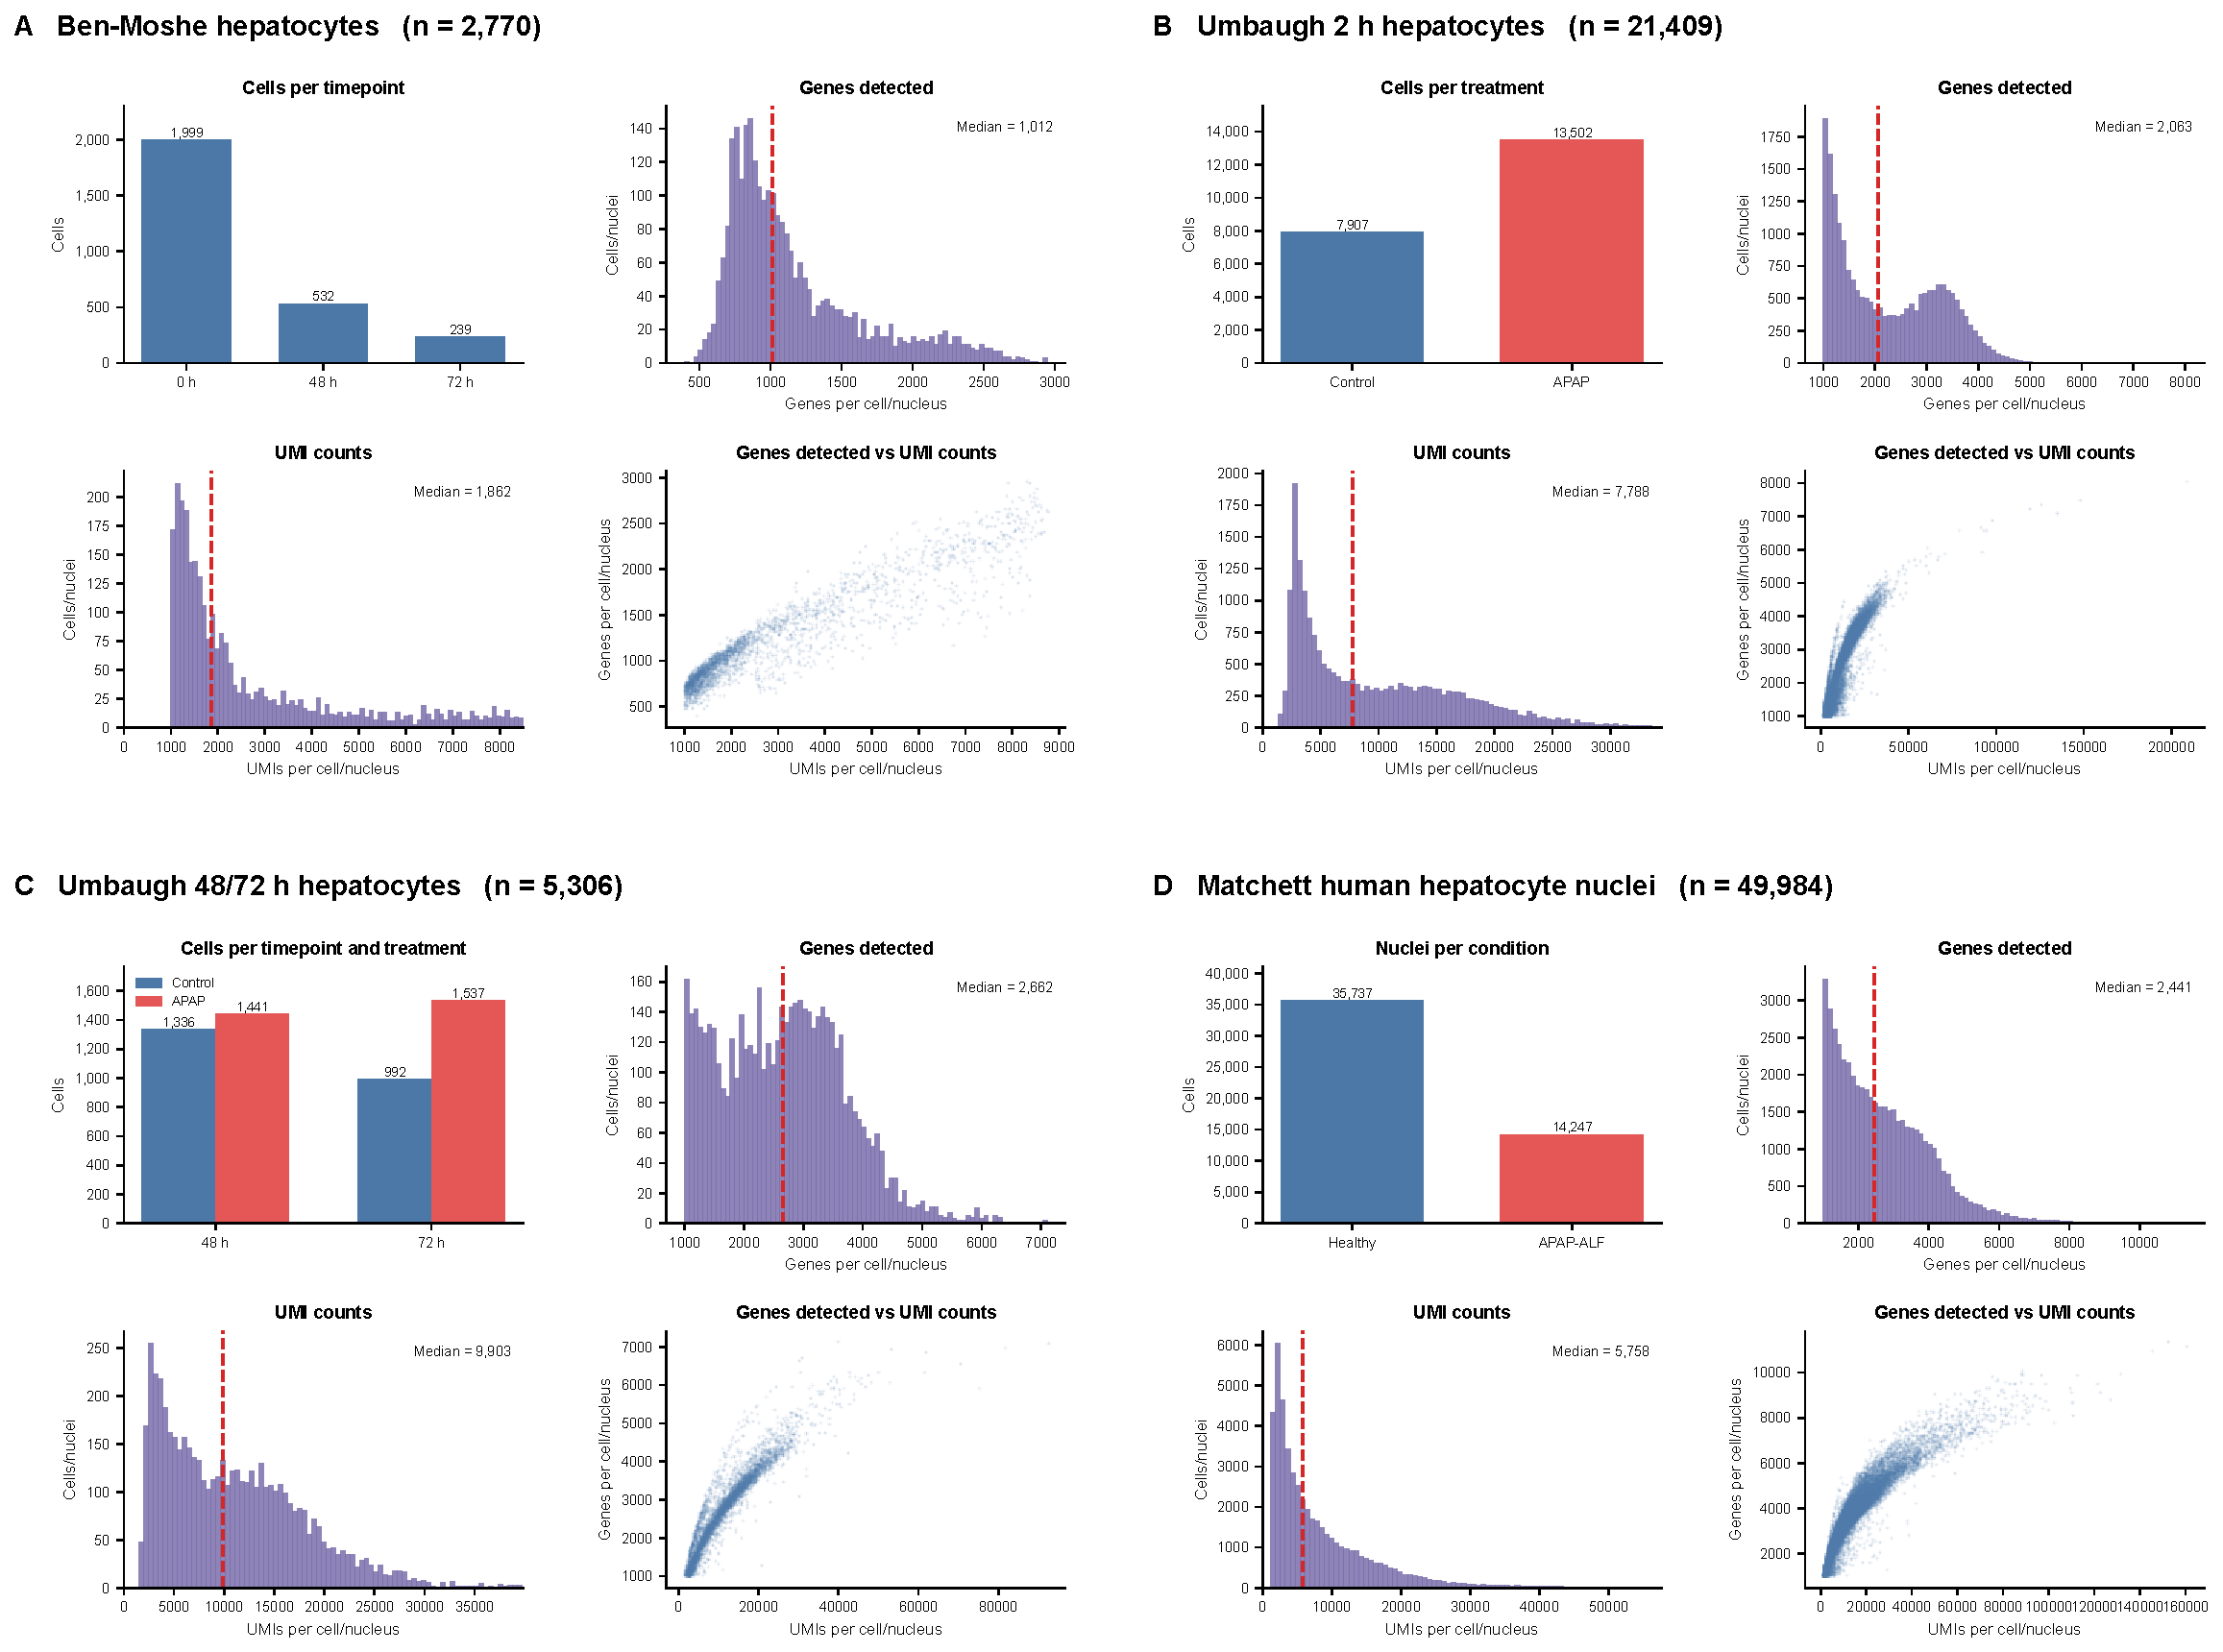
\includegraphics[width=\textwidth,trim={0.000bp 414.430bp 557.867bp 0.000bp},clip]{figures/figure_S1.pdf}
\caption{\textbf{\FigSOneTitle{}} \textbf{(A)} \FigSOneA{} \FigSOneNotes{}}
\label{fig:S1}
\end{figure}

\clearpage
\begin{figure}[H]
\centering
\ContinuedFloat
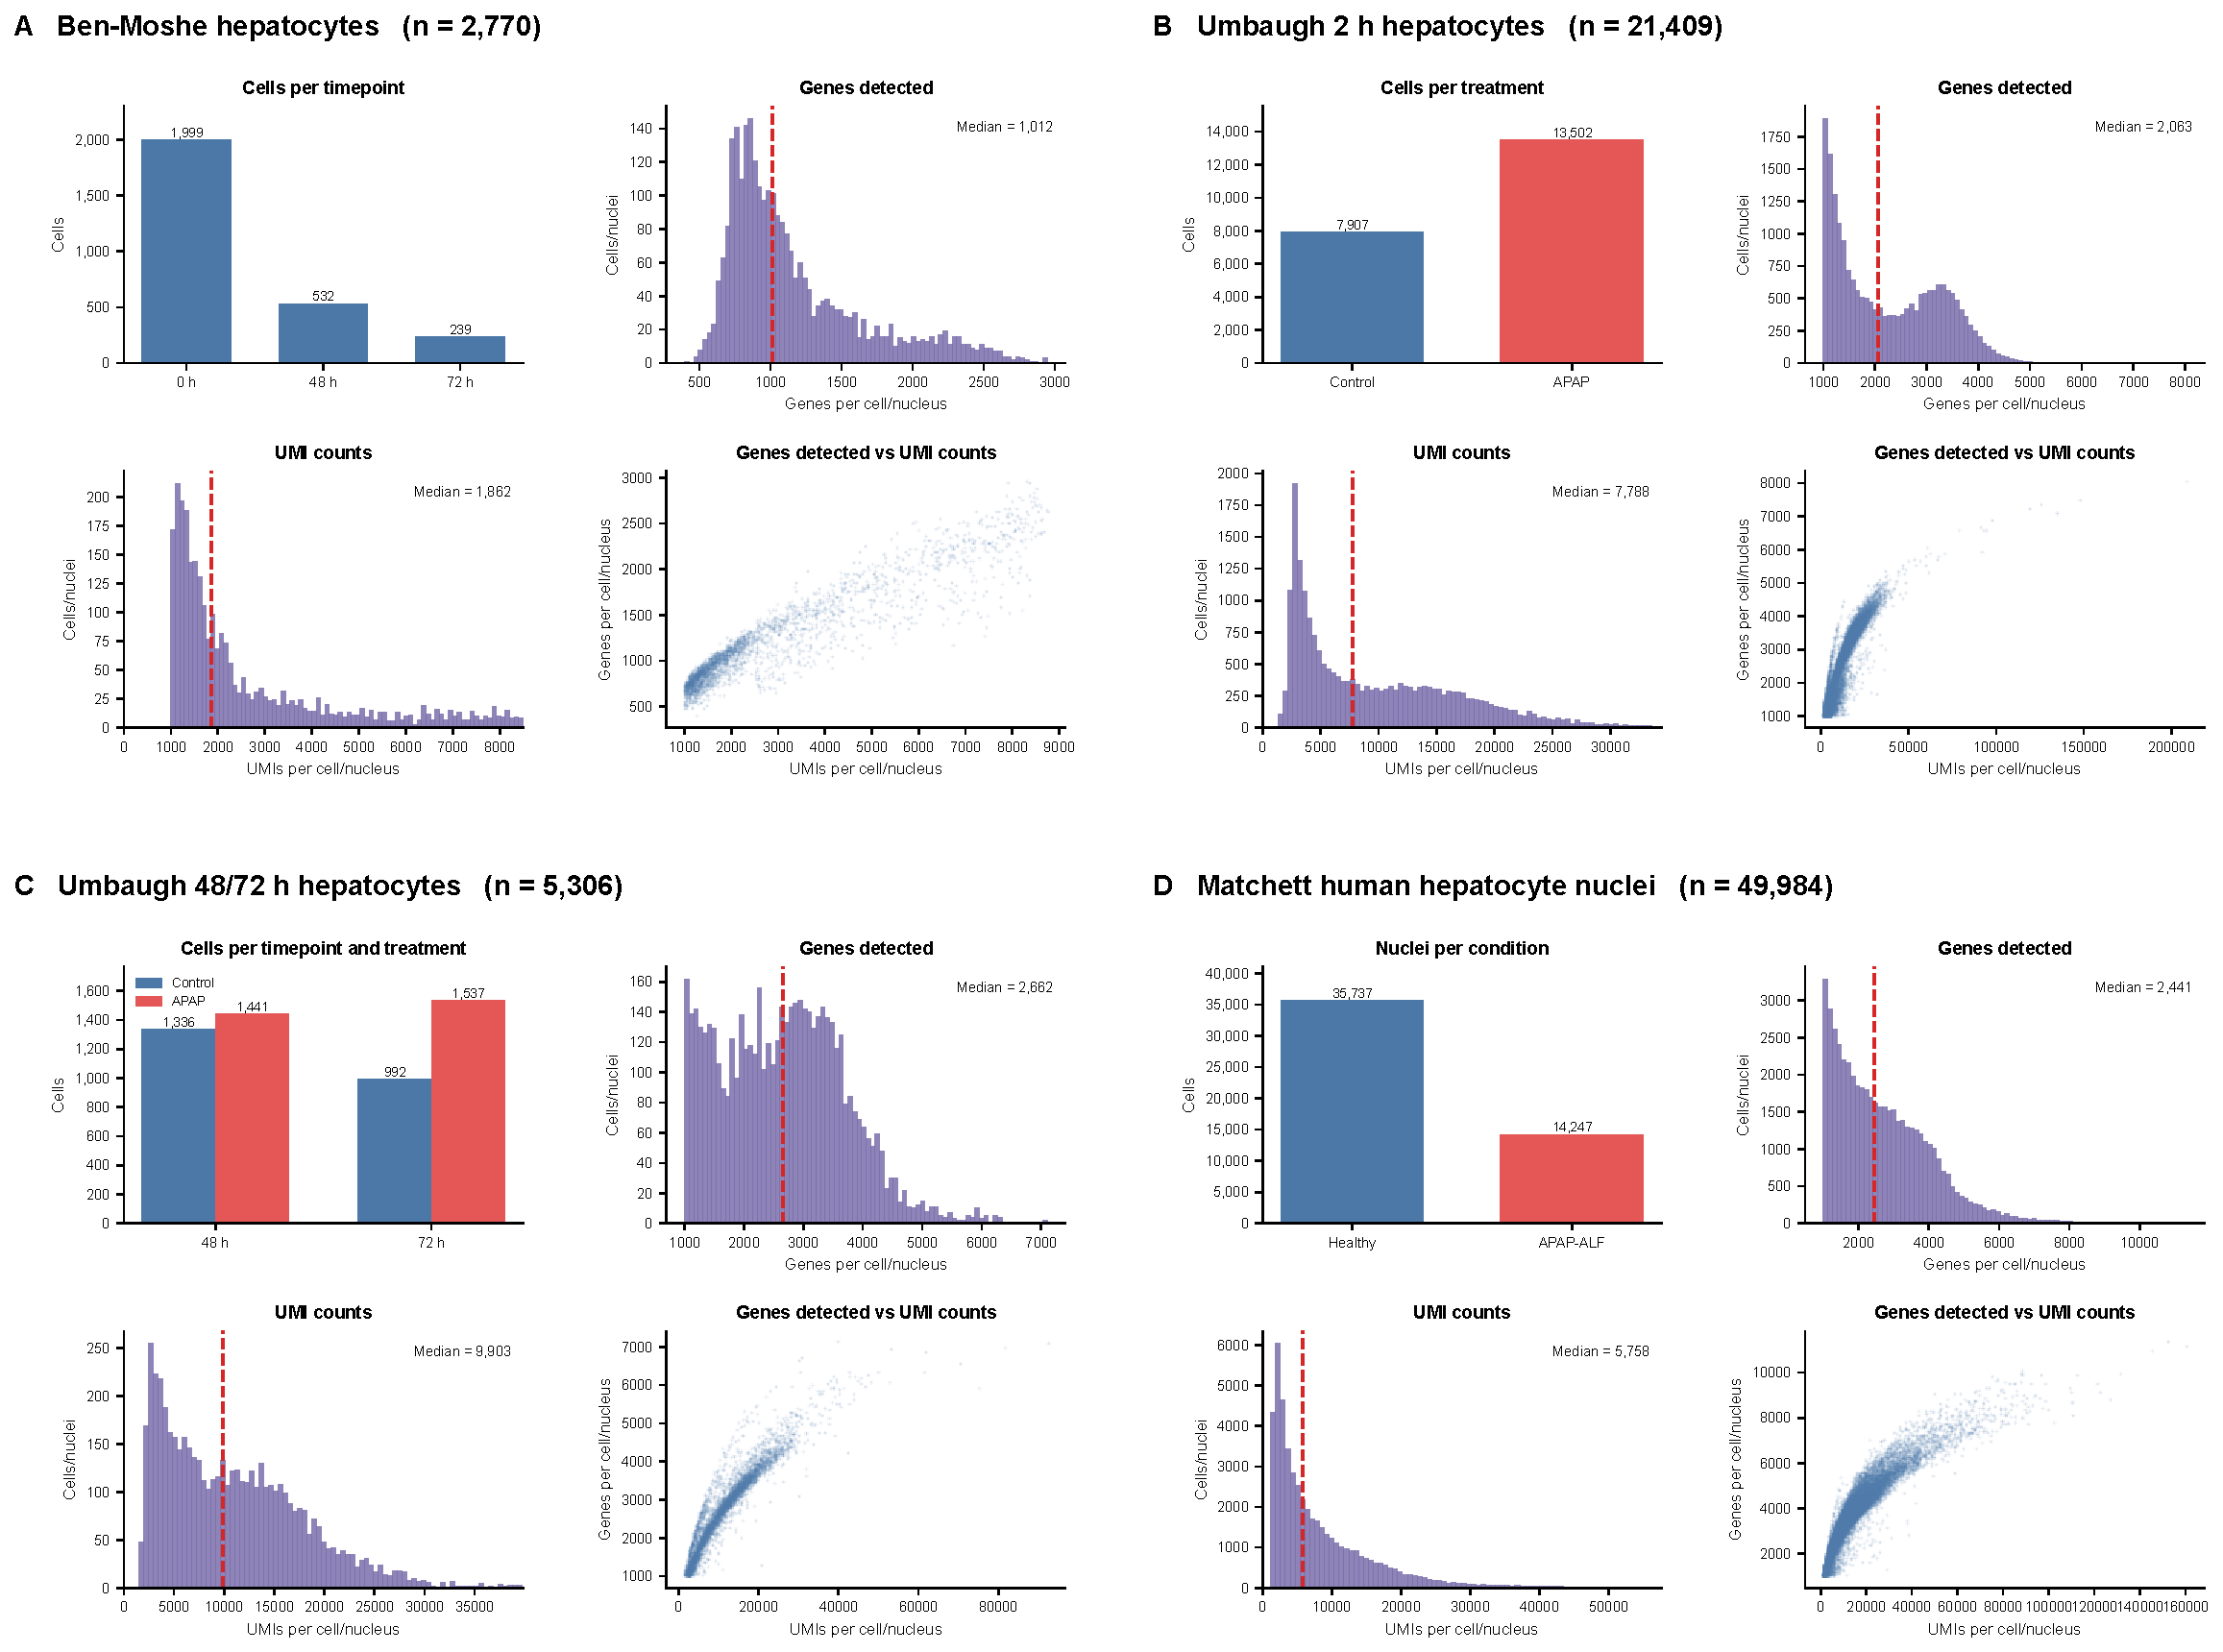
\includegraphics[width=\textwidth,trim={557.000bp 414.430bp 0.000bp 0.000bp},clip]{figures/figure_S1.pdf}
\caption{\textbf{\FigSOneTitle{} (continued)} \textbf{(B)} \FigSOneB{}}
\end{figure}

\clearpage
\begin{figure}[H]
\centering
\ContinuedFloat
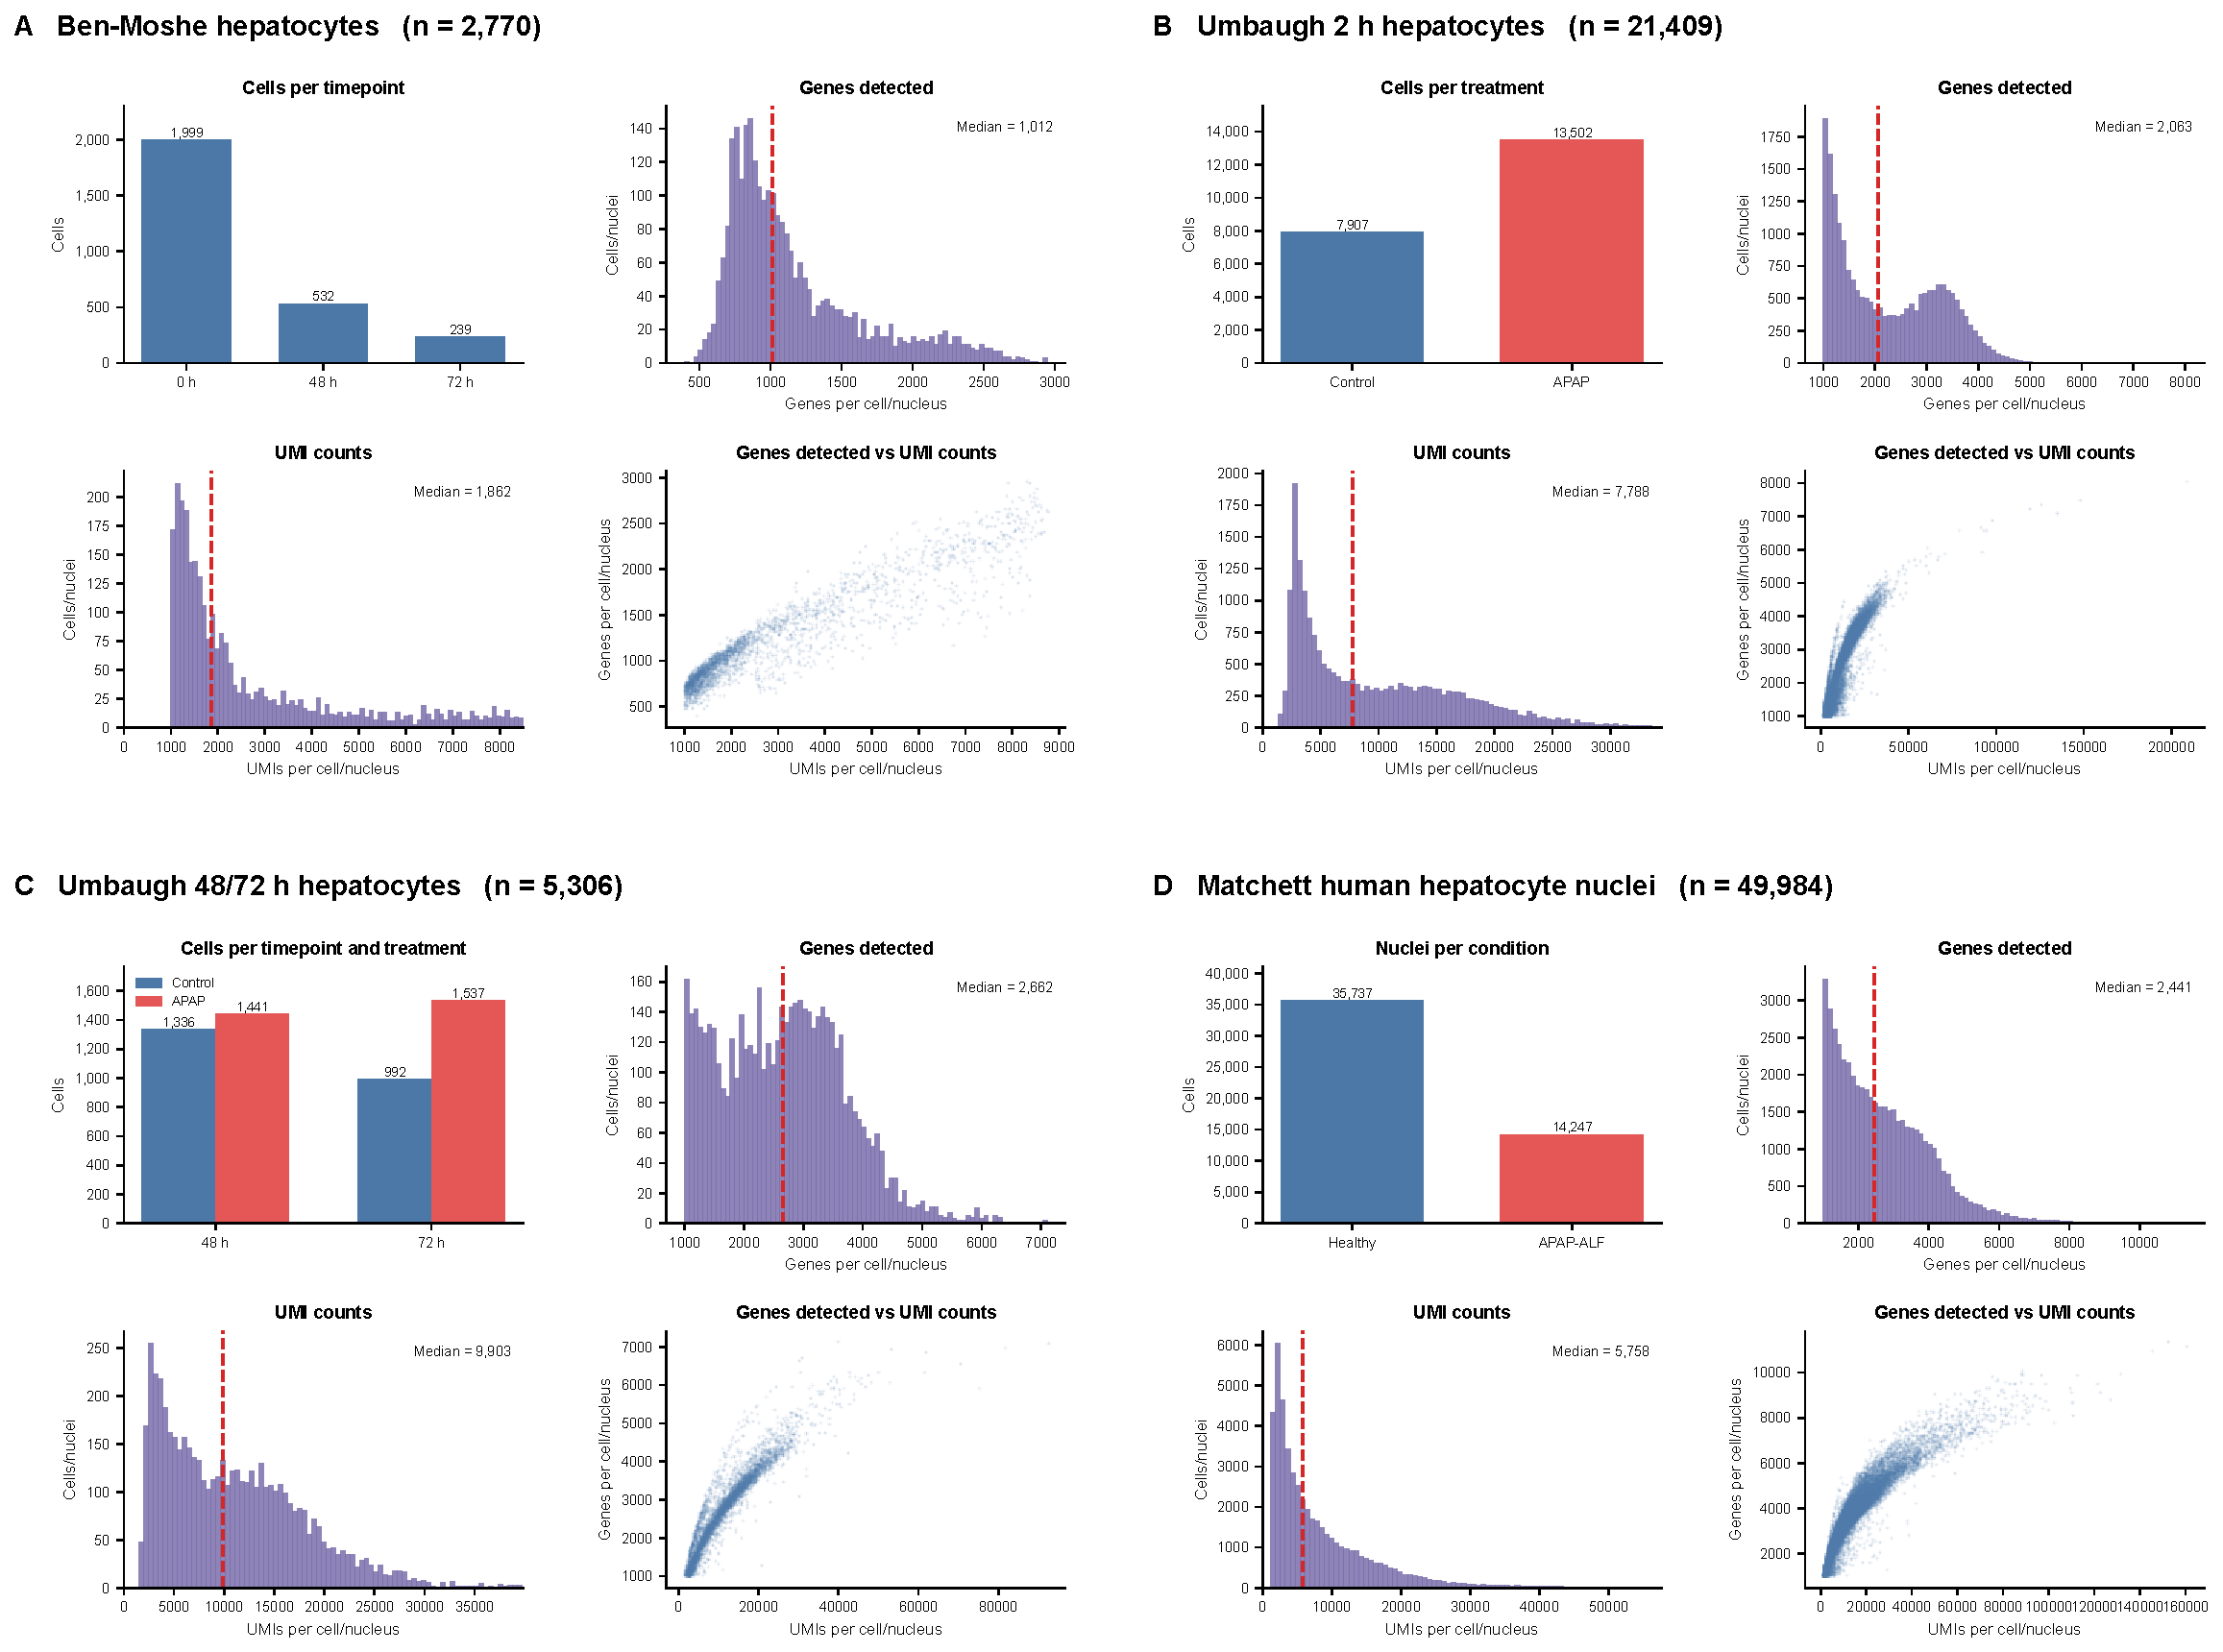
\includegraphics[width=\textwidth,trim={0.000bp 0.000bp 557.867bp 414.000bp},clip]{figures/figure_S1.pdf}
\caption{\textbf{\FigSOneTitle{} (continued)} \textbf{(C)} \FigSOneC{}}
\end{figure}

\clearpage
\begin{figure}[H]
\centering
\ContinuedFloat
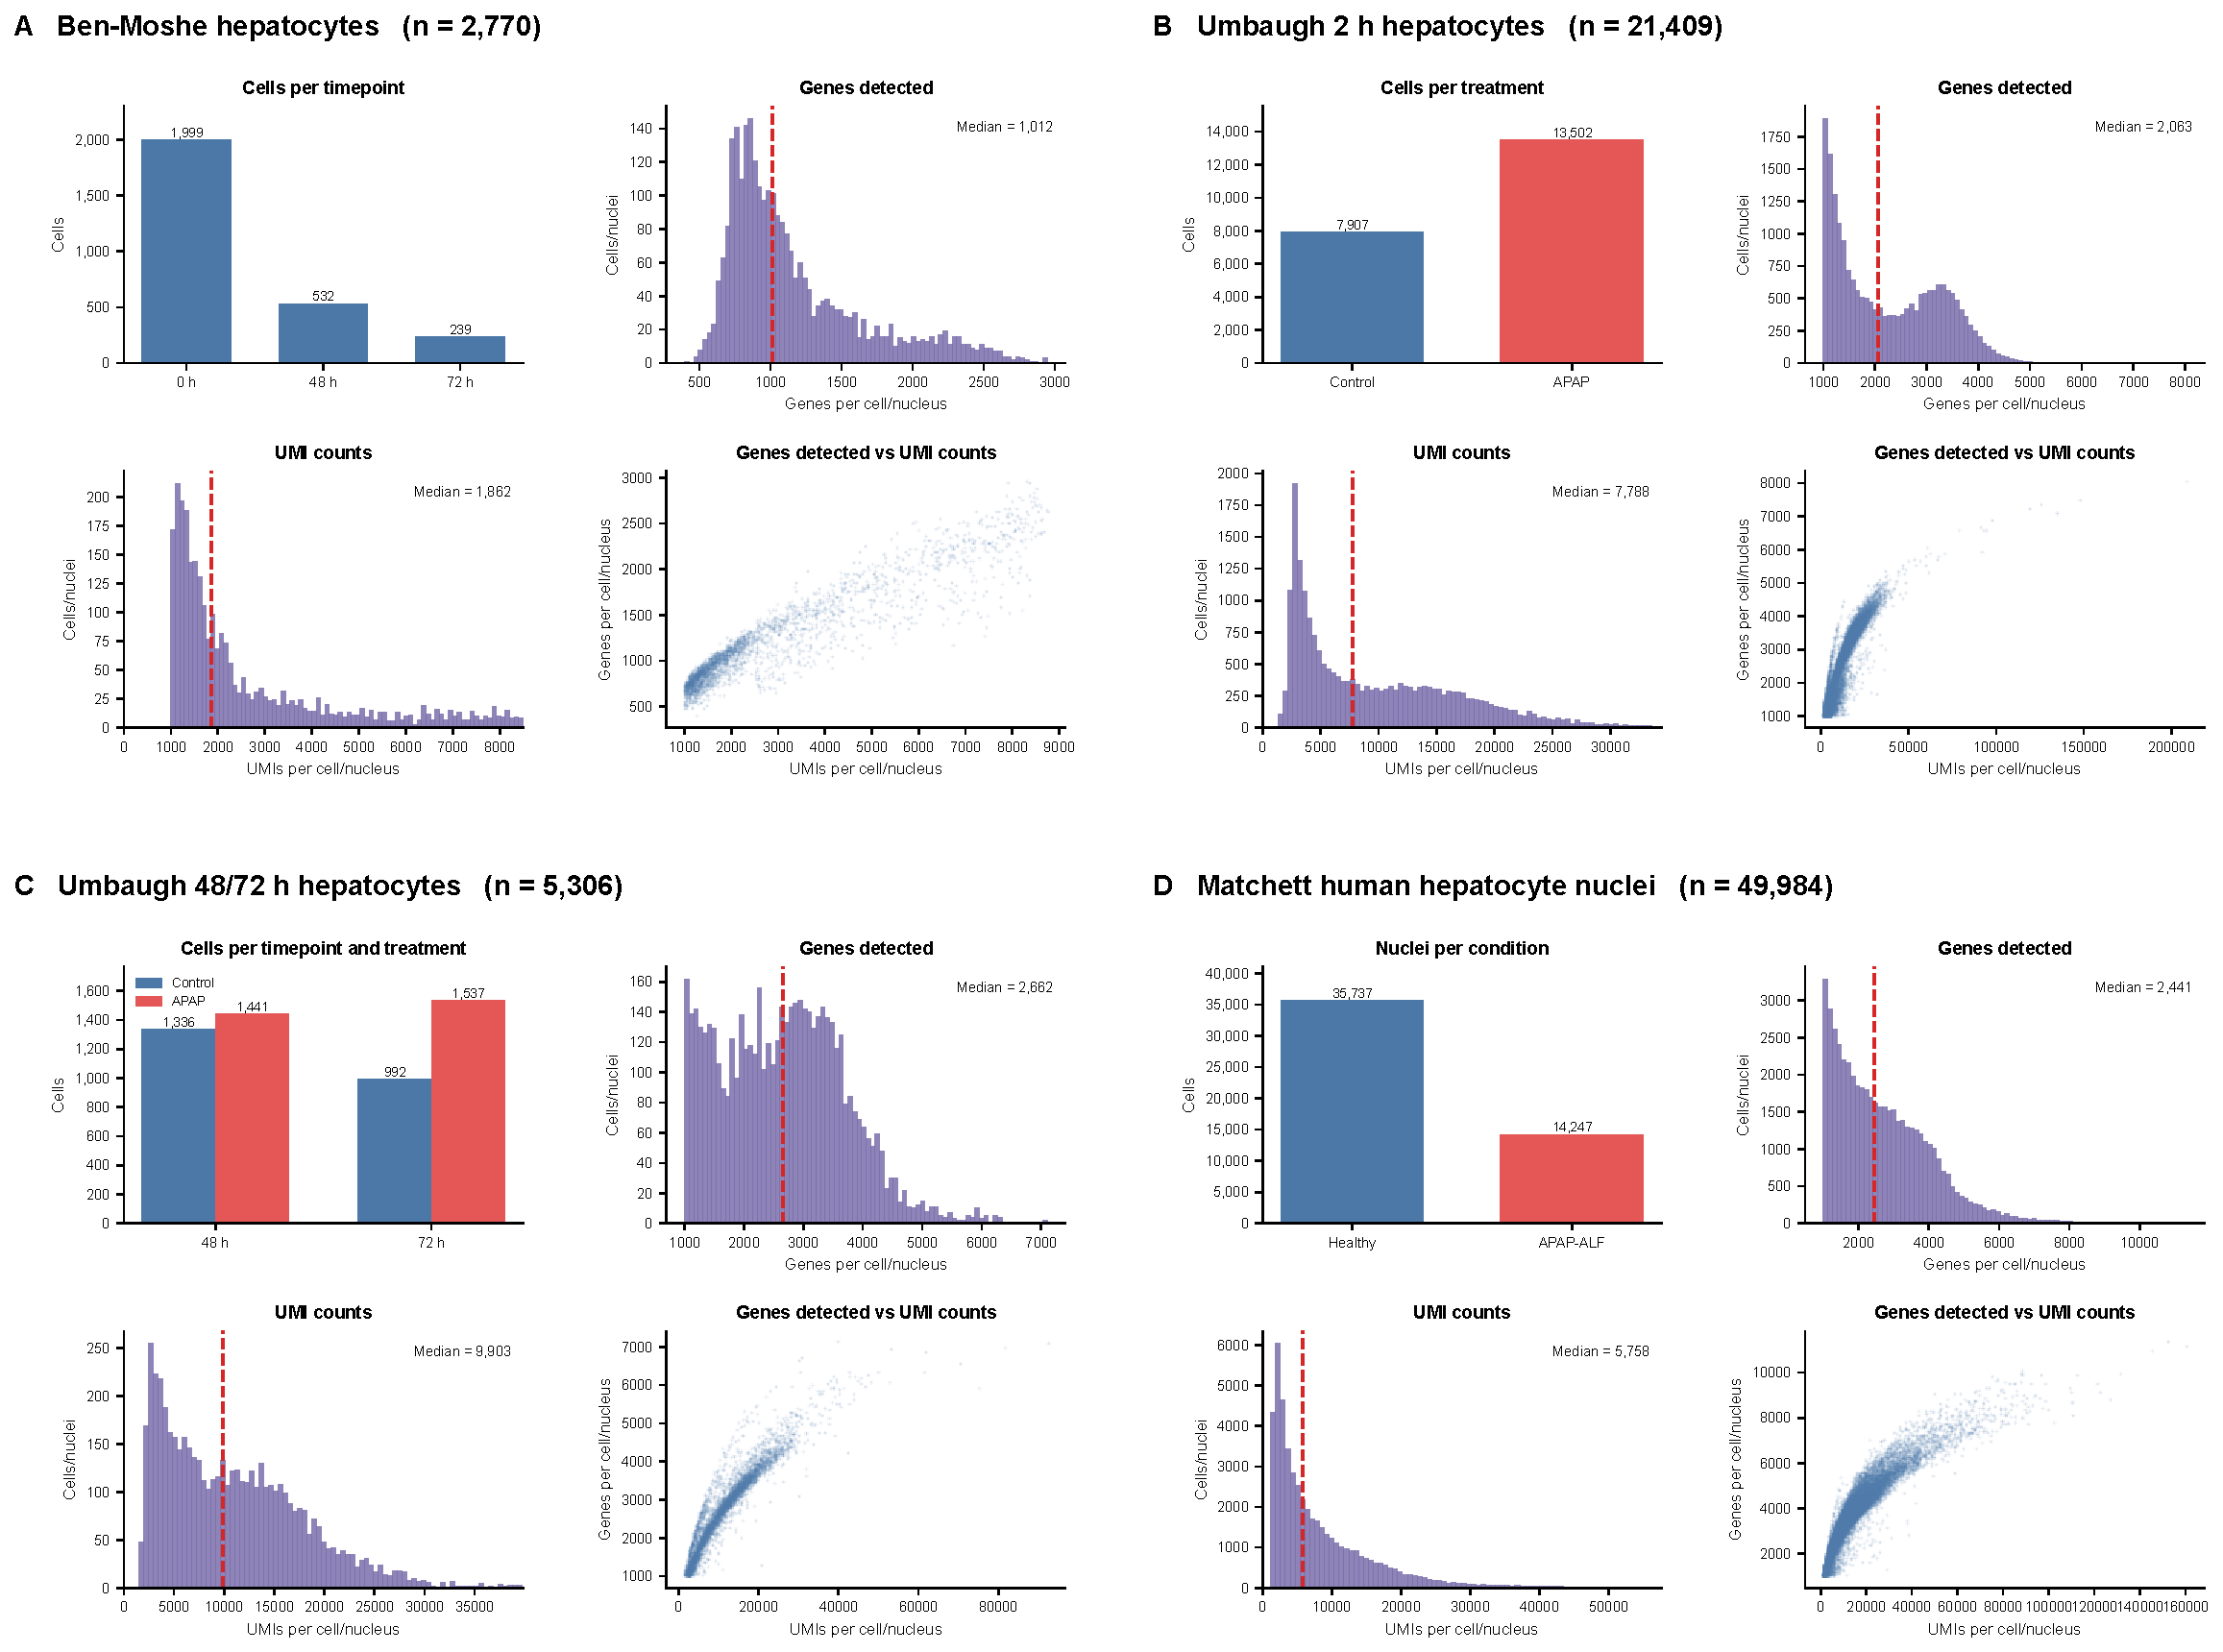
\includegraphics[width=\textwidth,trim={557.000bp 0.000bp 0.000bp 414.000bp},clip]{figures/figure_S1.pdf}
\caption{\textbf{\FigSOneTitle{} (continued)} \textbf{(D)} \FigSOneD{}}
\end{figure}

\clearpage
\begin{figure}[H]
\centering
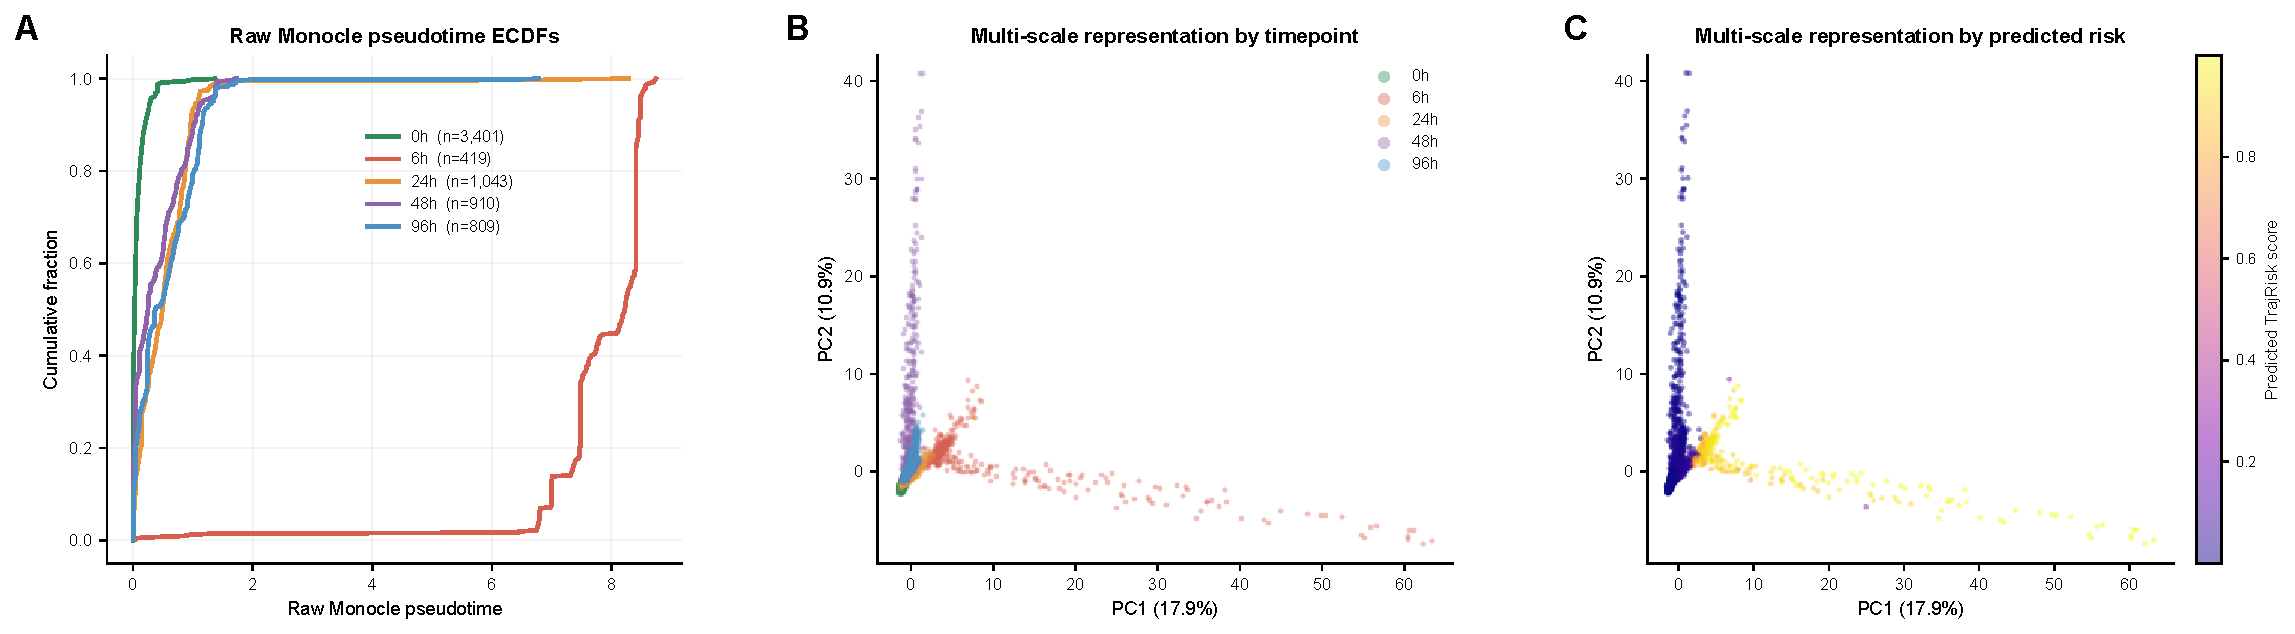
\includegraphics[width=0.78\textwidth,trim={0.000bp 0.000bp 734.759bp 0.000bp},clip]{figures/figure_S2.pdf}
\caption{\textbf{\FigSTwoTitle{}} \textbf{(A)} \FigSTwoA{} \FigSTwoNotes{}}
\label{fig:S2}
\end{figure}

\clearpage
\begin{figure}[H]
\centering
\ContinuedFloat
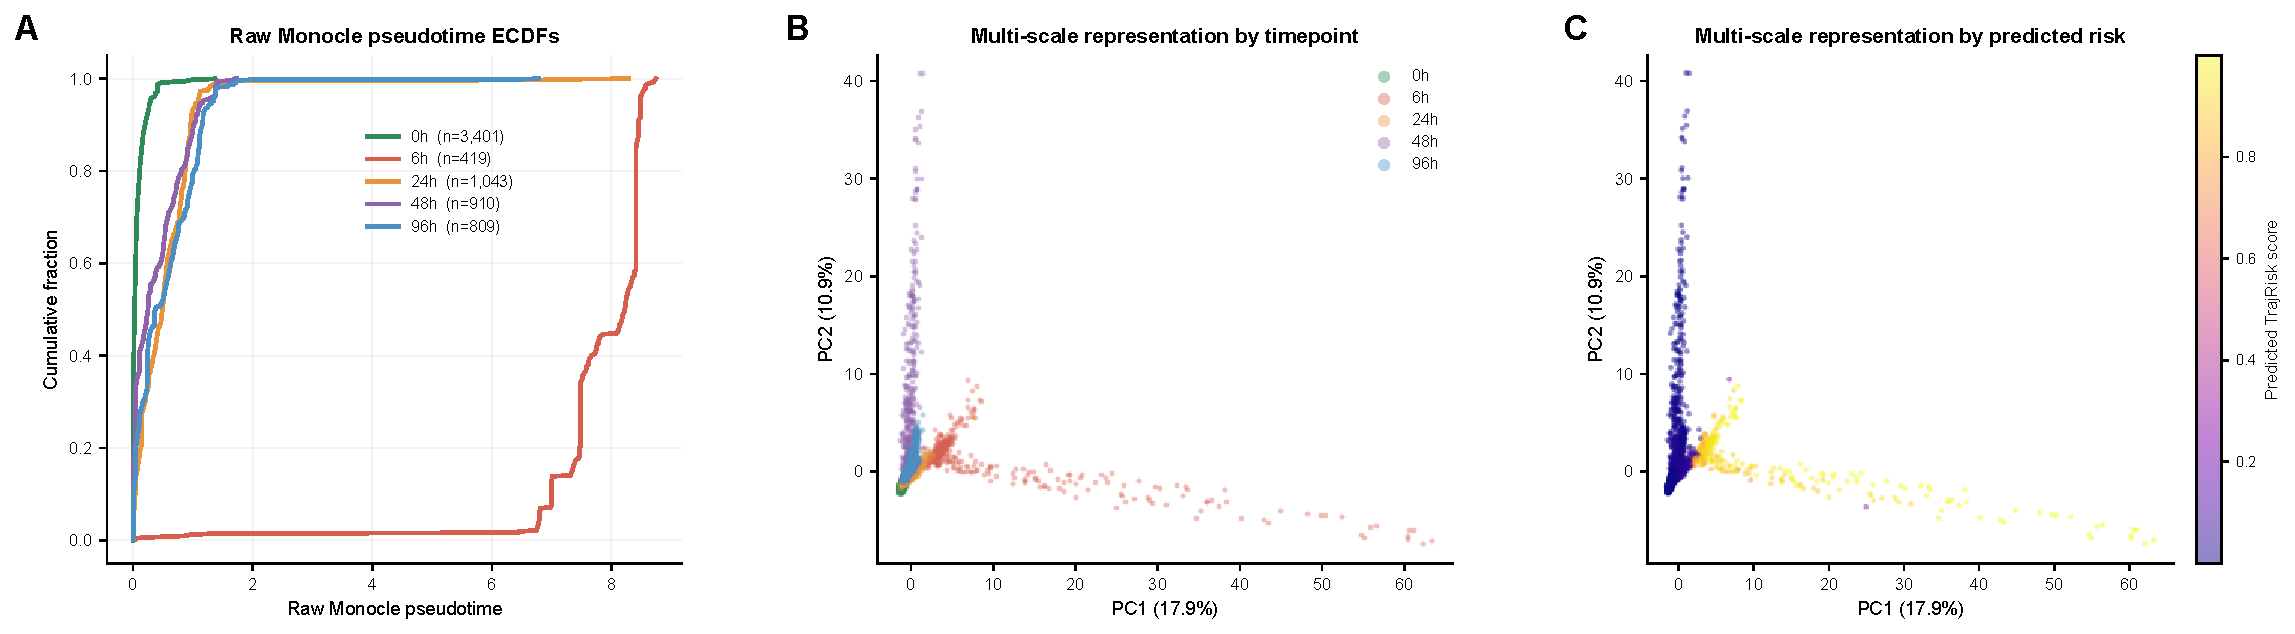
\includegraphics[width=0.64\textwidth,trim={369.000bp 0.000bp 366.759bp 0.000bp},clip]{figures/figure_S2.pdf}
\par\vspace{12pt}
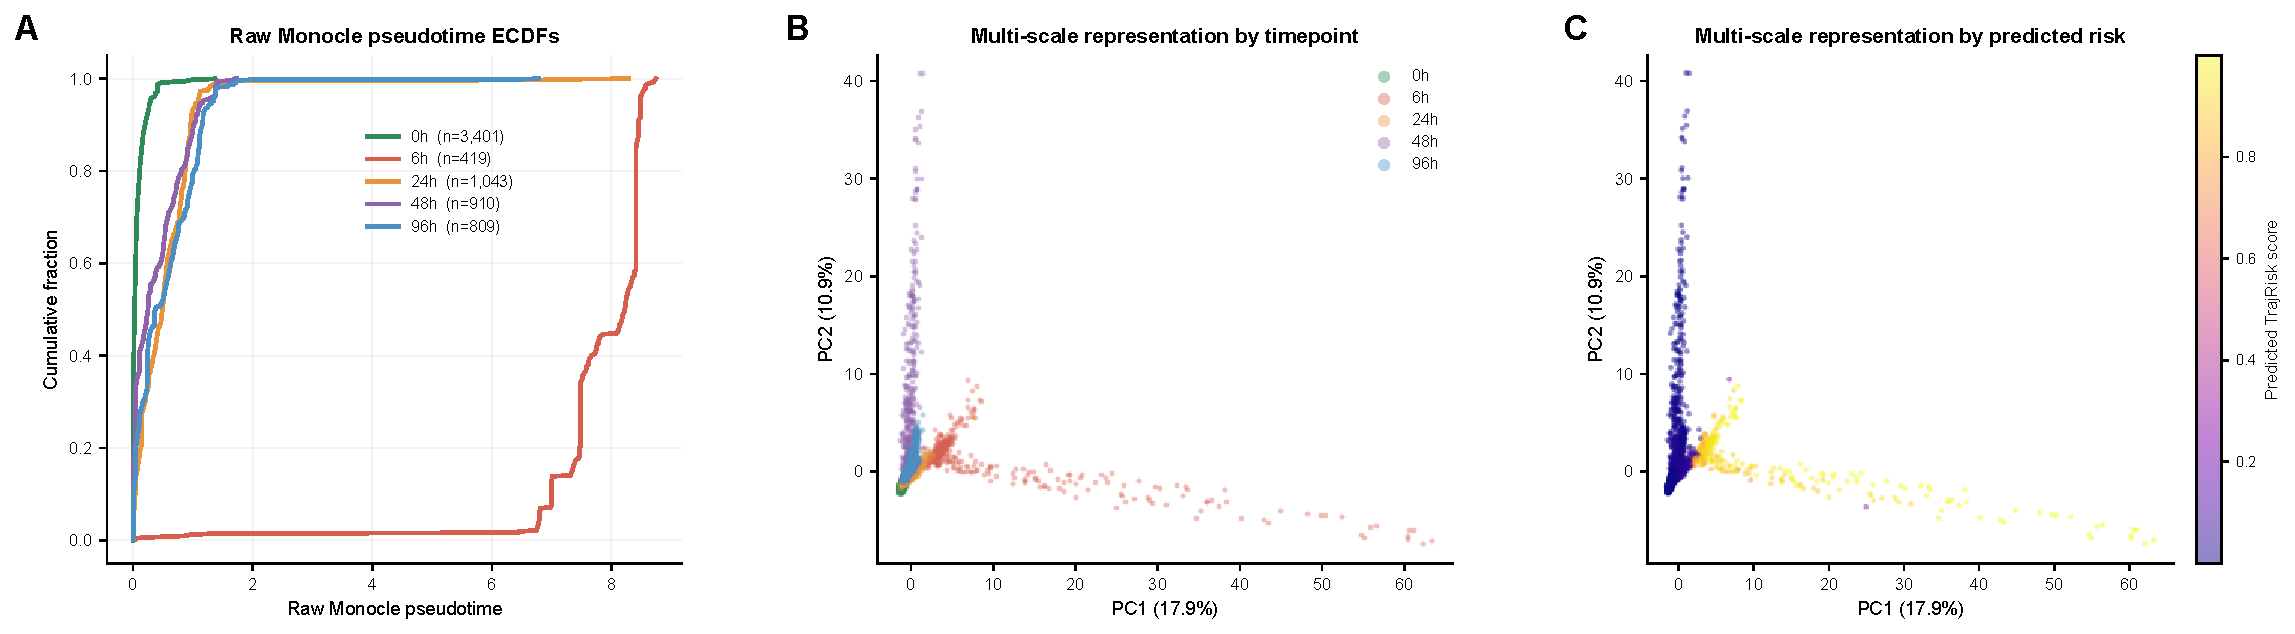
\includegraphics[width=0.64\textwidth,trim={737.000bp 0.000bp 0.000bp 0.000bp},clip]{figures/figure_S2.pdf}
\caption{\textbf{\FigSTwoTitle{} (continued)} \textbf{(B)} \FigSTwoB{} \textbf{(C)} \FigSTwoC{}}
\end{figure}

\clearpage
\begin{figure}[H]
\centering
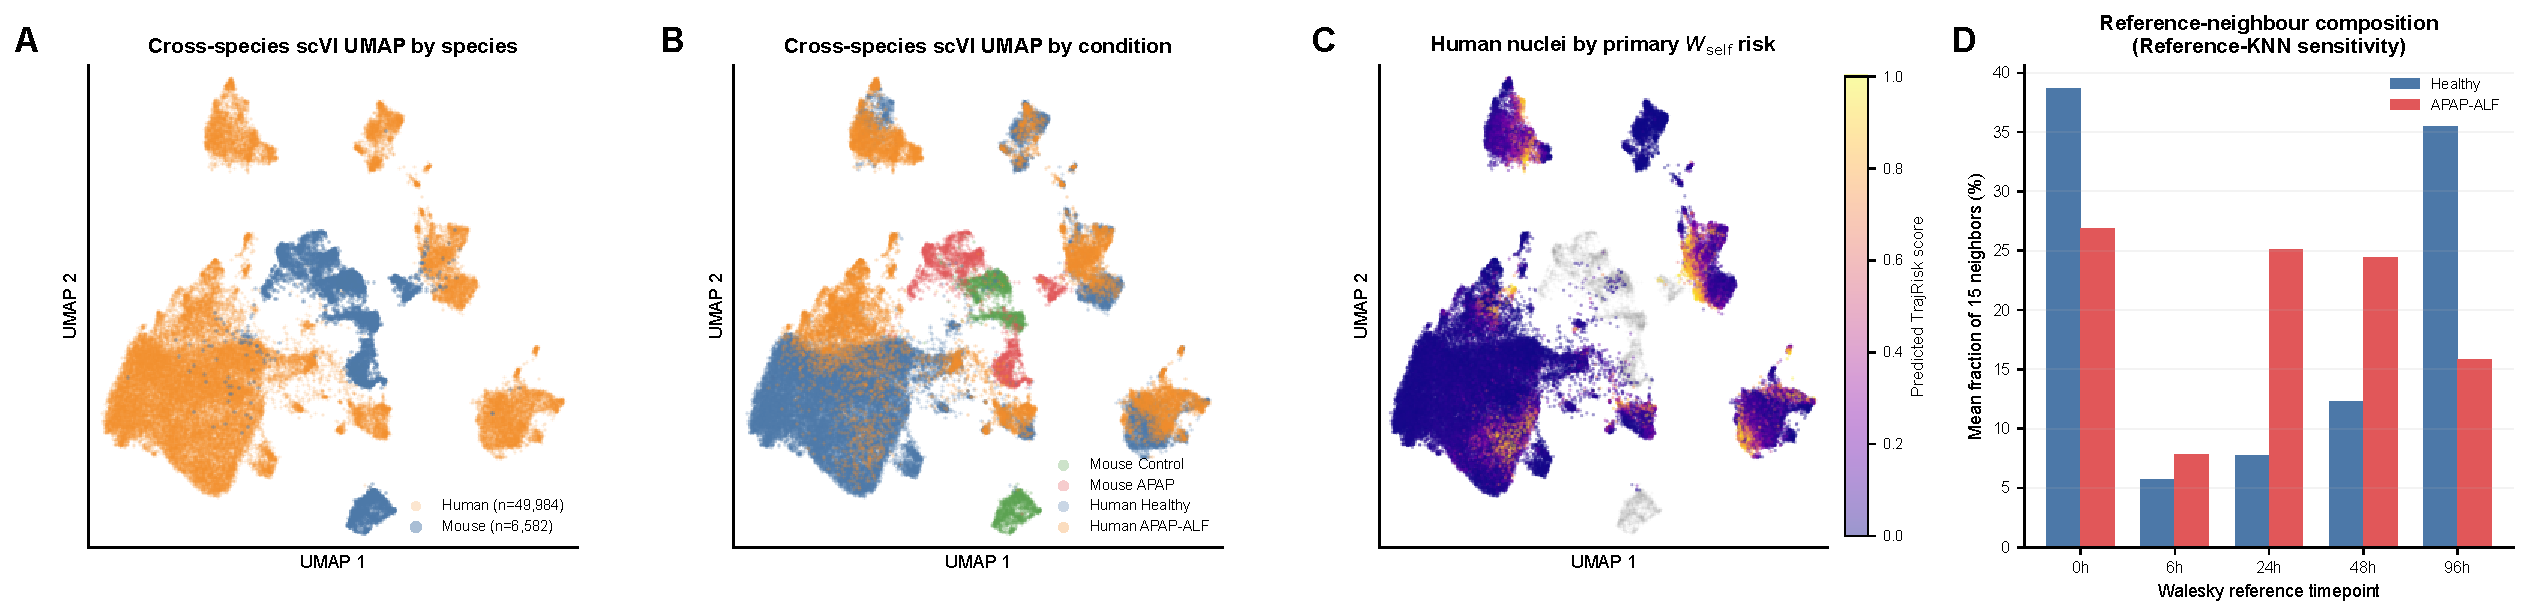
\includegraphics[width=0.492\textwidth,trim={0.000bp 0.000bp 911.701bp 0.000bp},clip]{figures/figure_S3.pdf}\hfill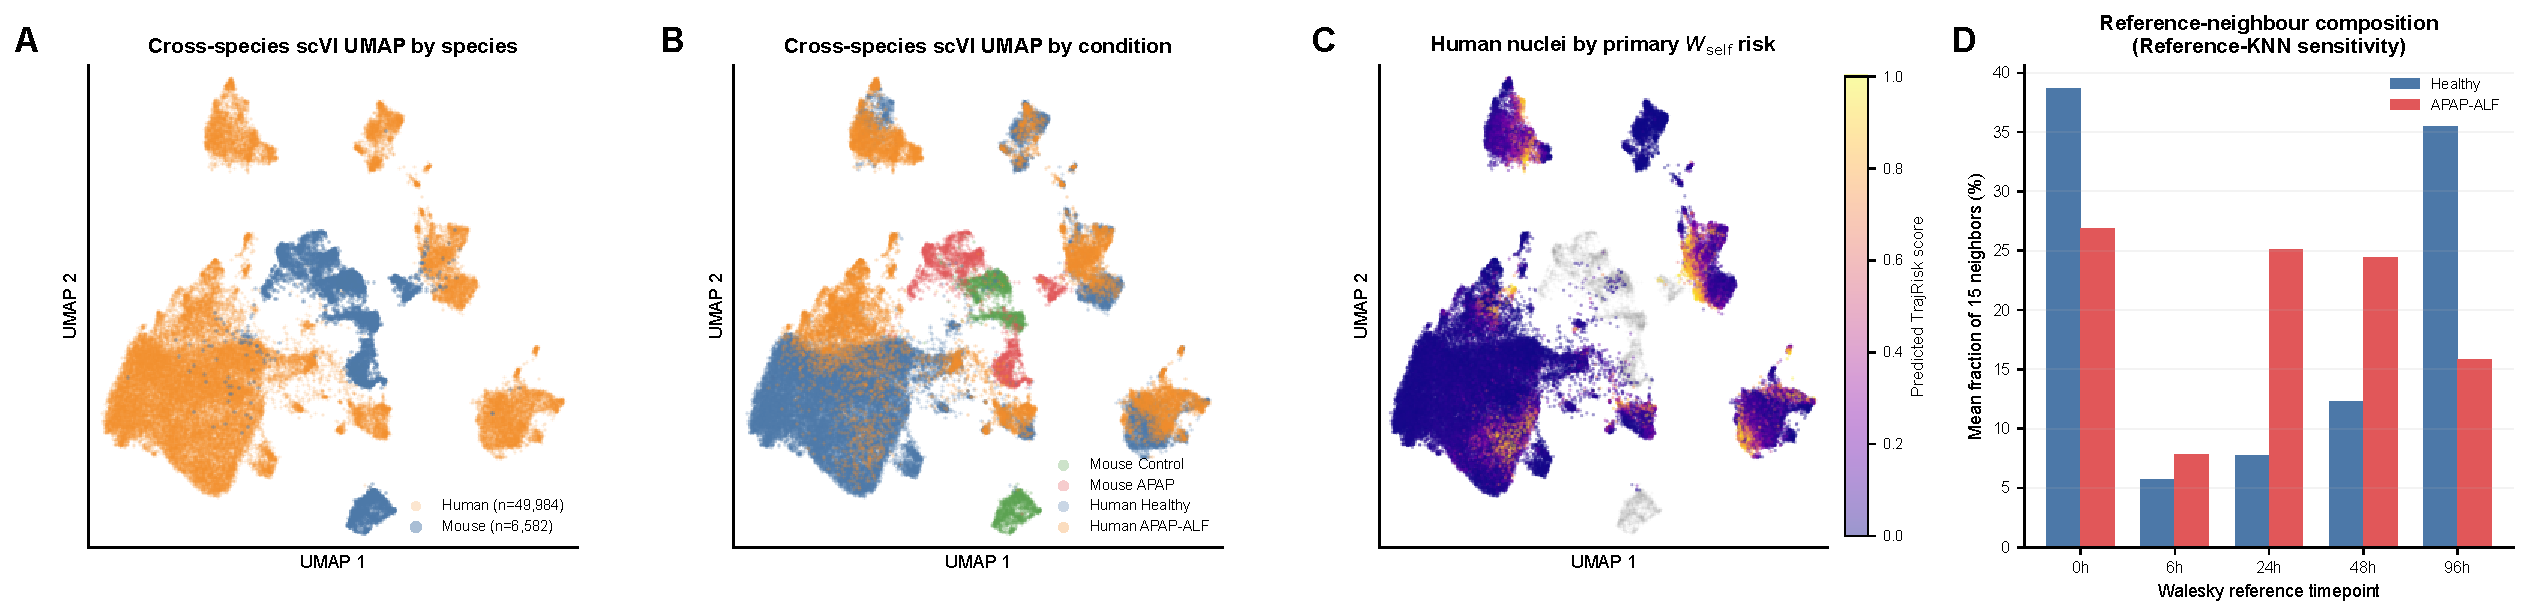
\includegraphics[width=0.492\textwidth,trim={303.000bp 0.000bp 607.701bp 0.000bp},clip]{figures/figure_S3.pdf}
\par\vspace{12pt}
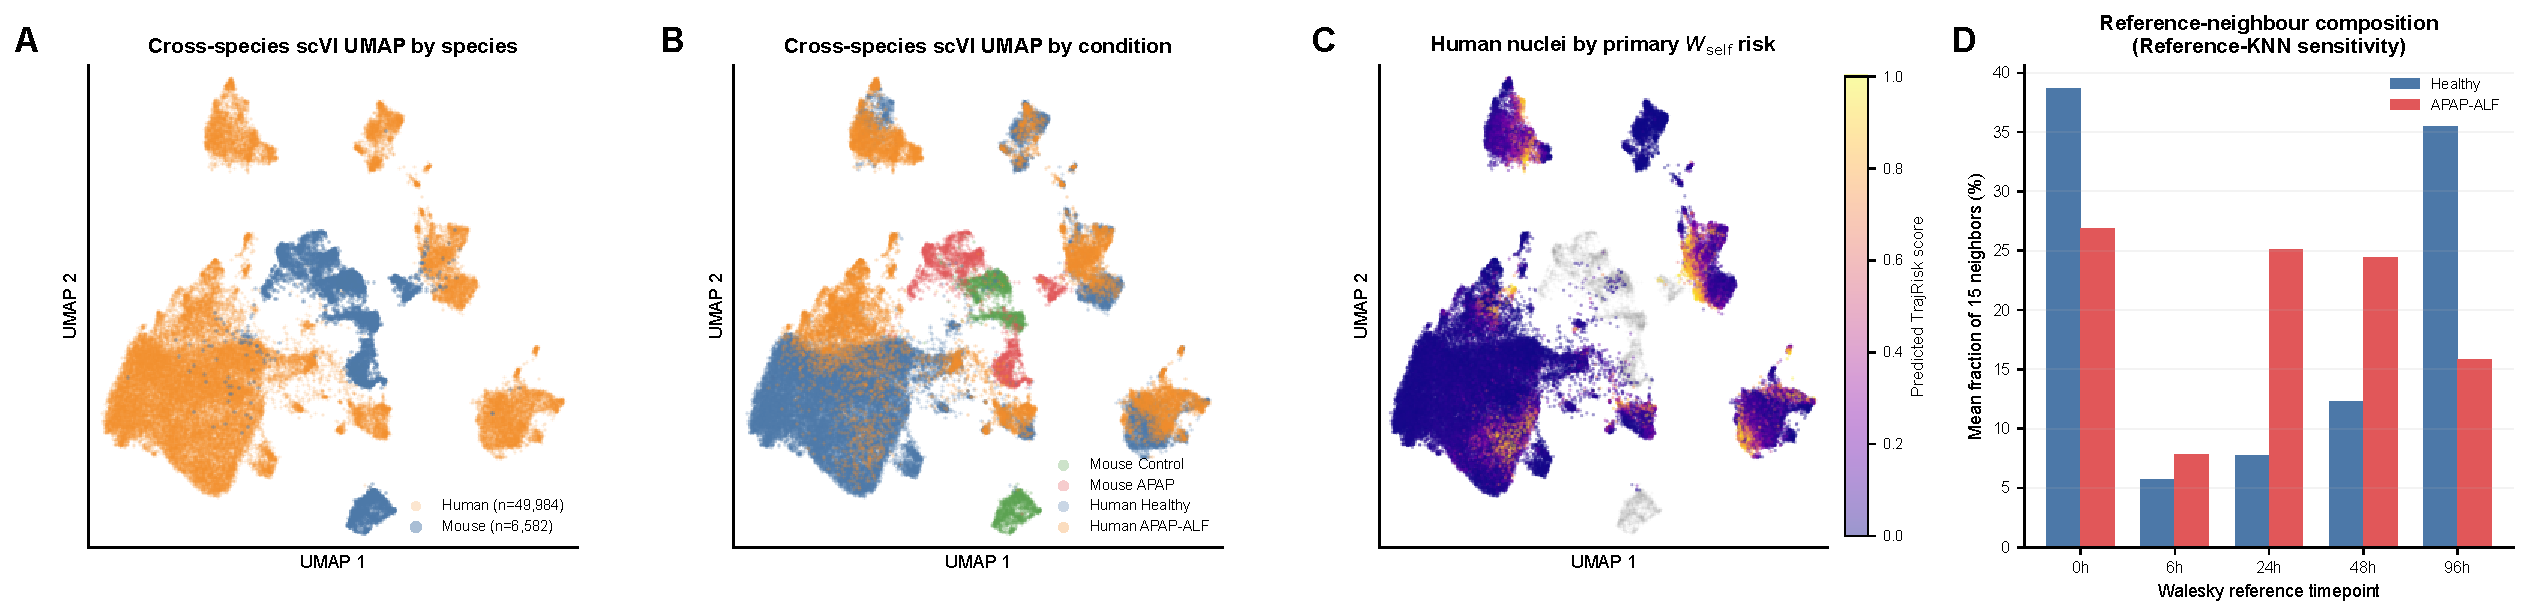
\includegraphics[width=0.526\textwidth,trim={607.000bp 0.000bp 283.701bp 0.000bp},clip]{figures/figure_S3.pdf}\hfill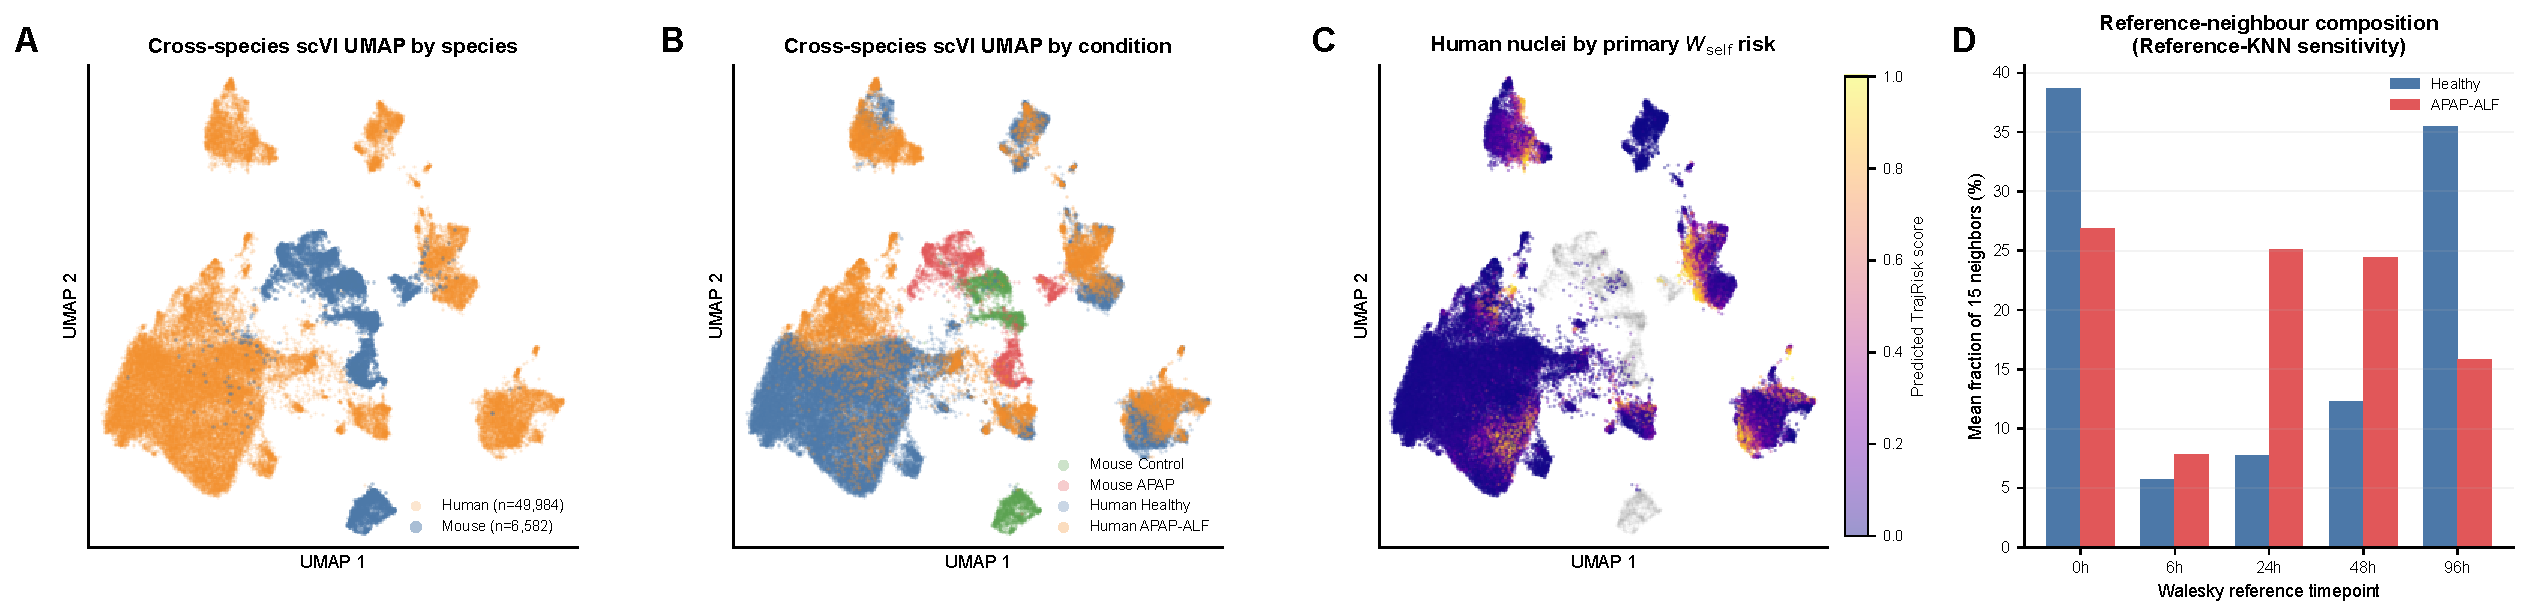
\includegraphics[width=0.460\textwidth,trim={931.000bp 0.000bp 0.000bp 0.000bp},clip]{figures/figure_S3.pdf}
\caption{\textbf{\FigSThreeTitle{}} \textbf{(A)} \FigSThreeA{} \textbf{(B)} \FigSThreeB{} \textbf{(C)} \FigSThreeC{} \textbf{(D)} \FigSThreeD{} \FigSThreeNotes{}}
\label{fig:S3}
\end{figure}

\clearpage
\begin{figure}[H]
\centering
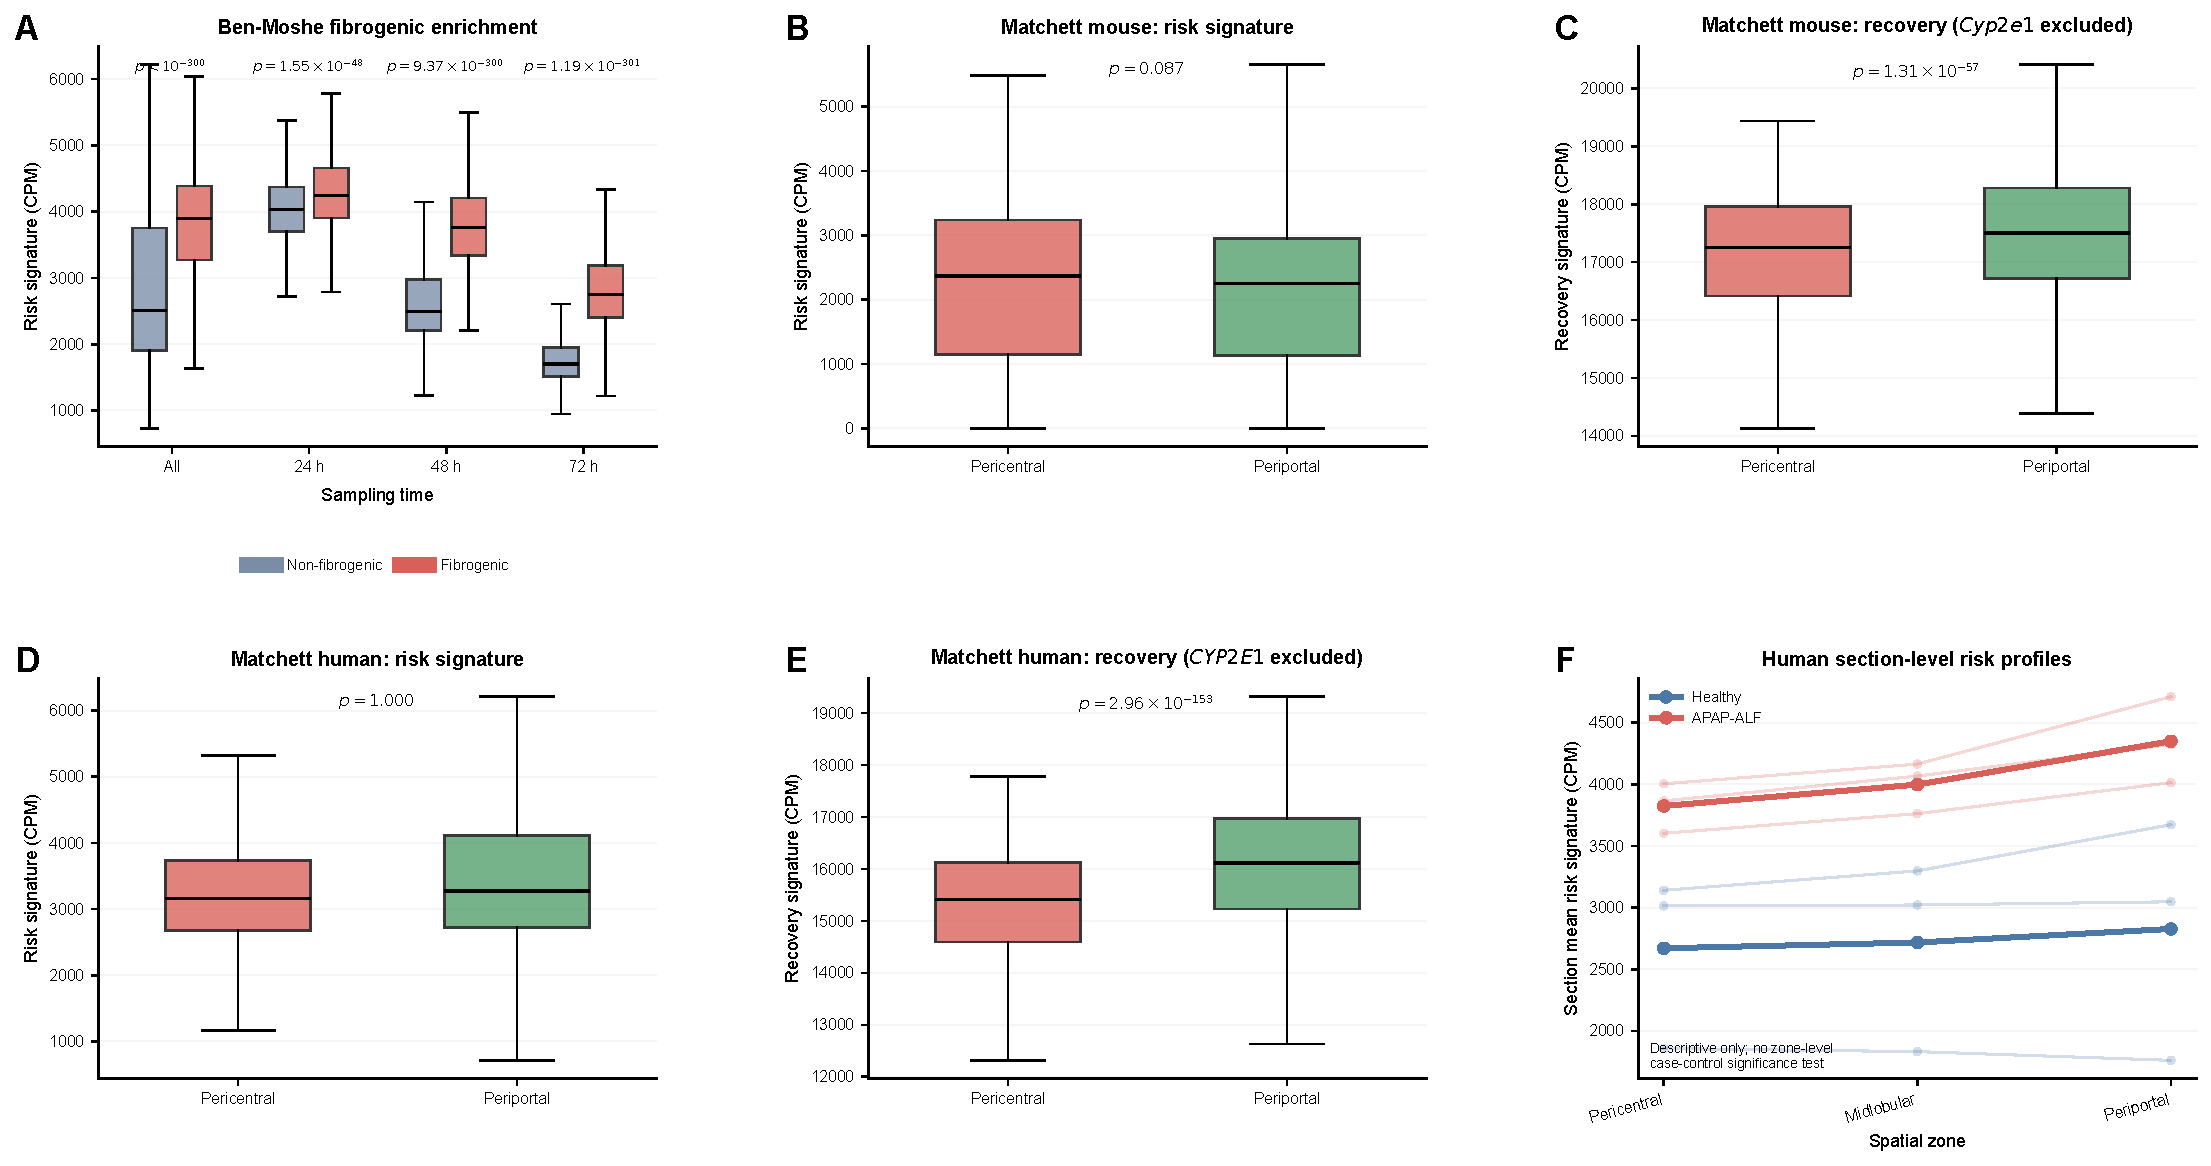
\includegraphics[width=0.74\textwidth,trim={0.000bp 286.872bp 706.415bp 0.000bp},clip]{figures/figure_S4.pdf}
\par\vspace{12pt}
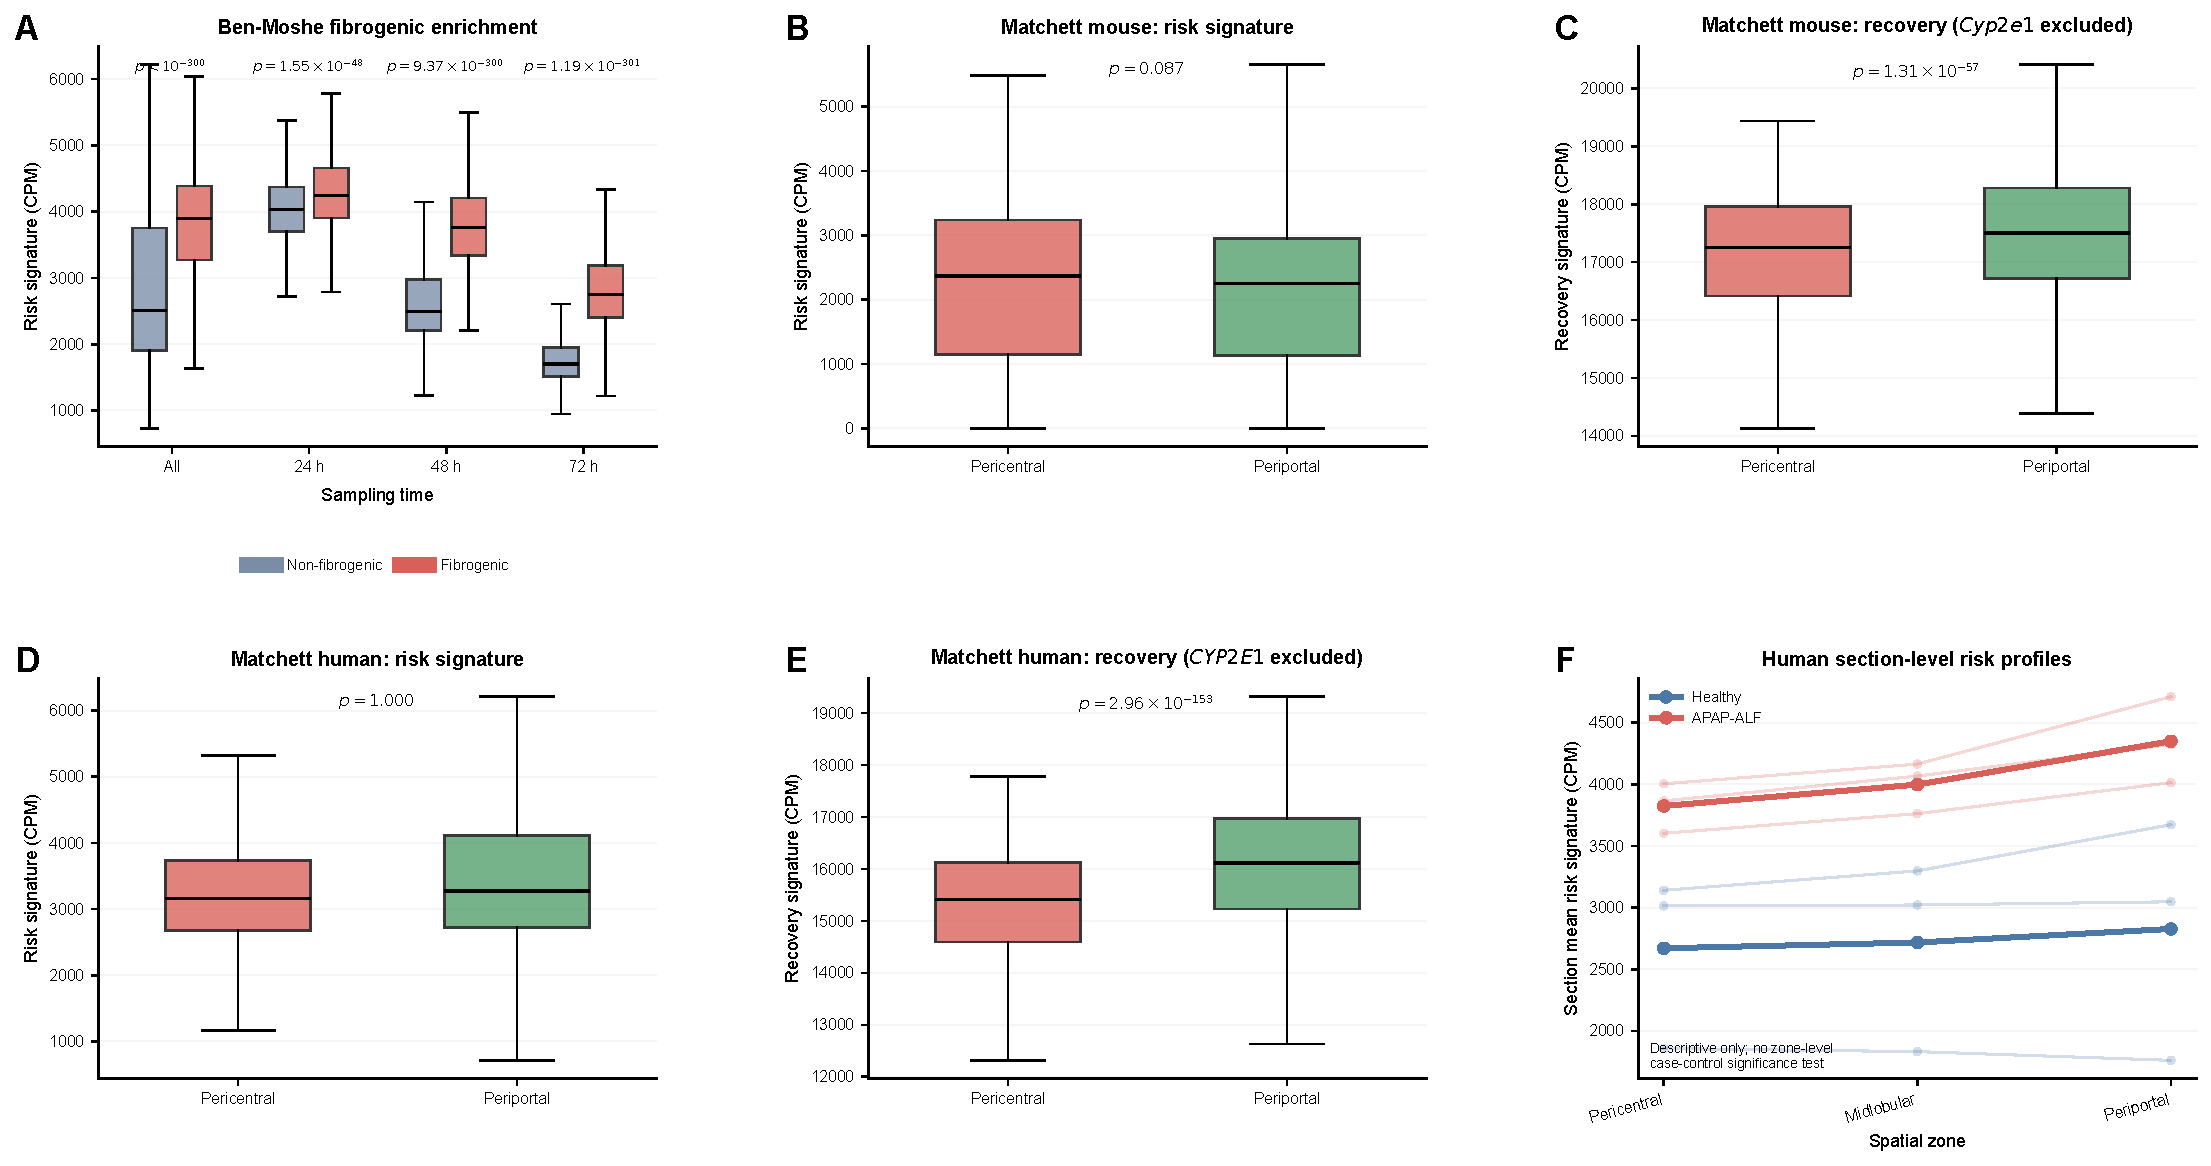
\includegraphics[width=0.64\textwidth,trim={356.000bp 286.872bp 354.415bp 0.000bp},clip]{figures/figure_S4.pdf}
\caption{\textbf{\FigSFourTitle{}} \textbf{(A)} \FigSFourA{} \textbf{(B)} \FigSFourB{}}
\label{fig:S4}
\end{figure}

\clearpage
\begin{figure}[H]
\centering
\ContinuedFloat
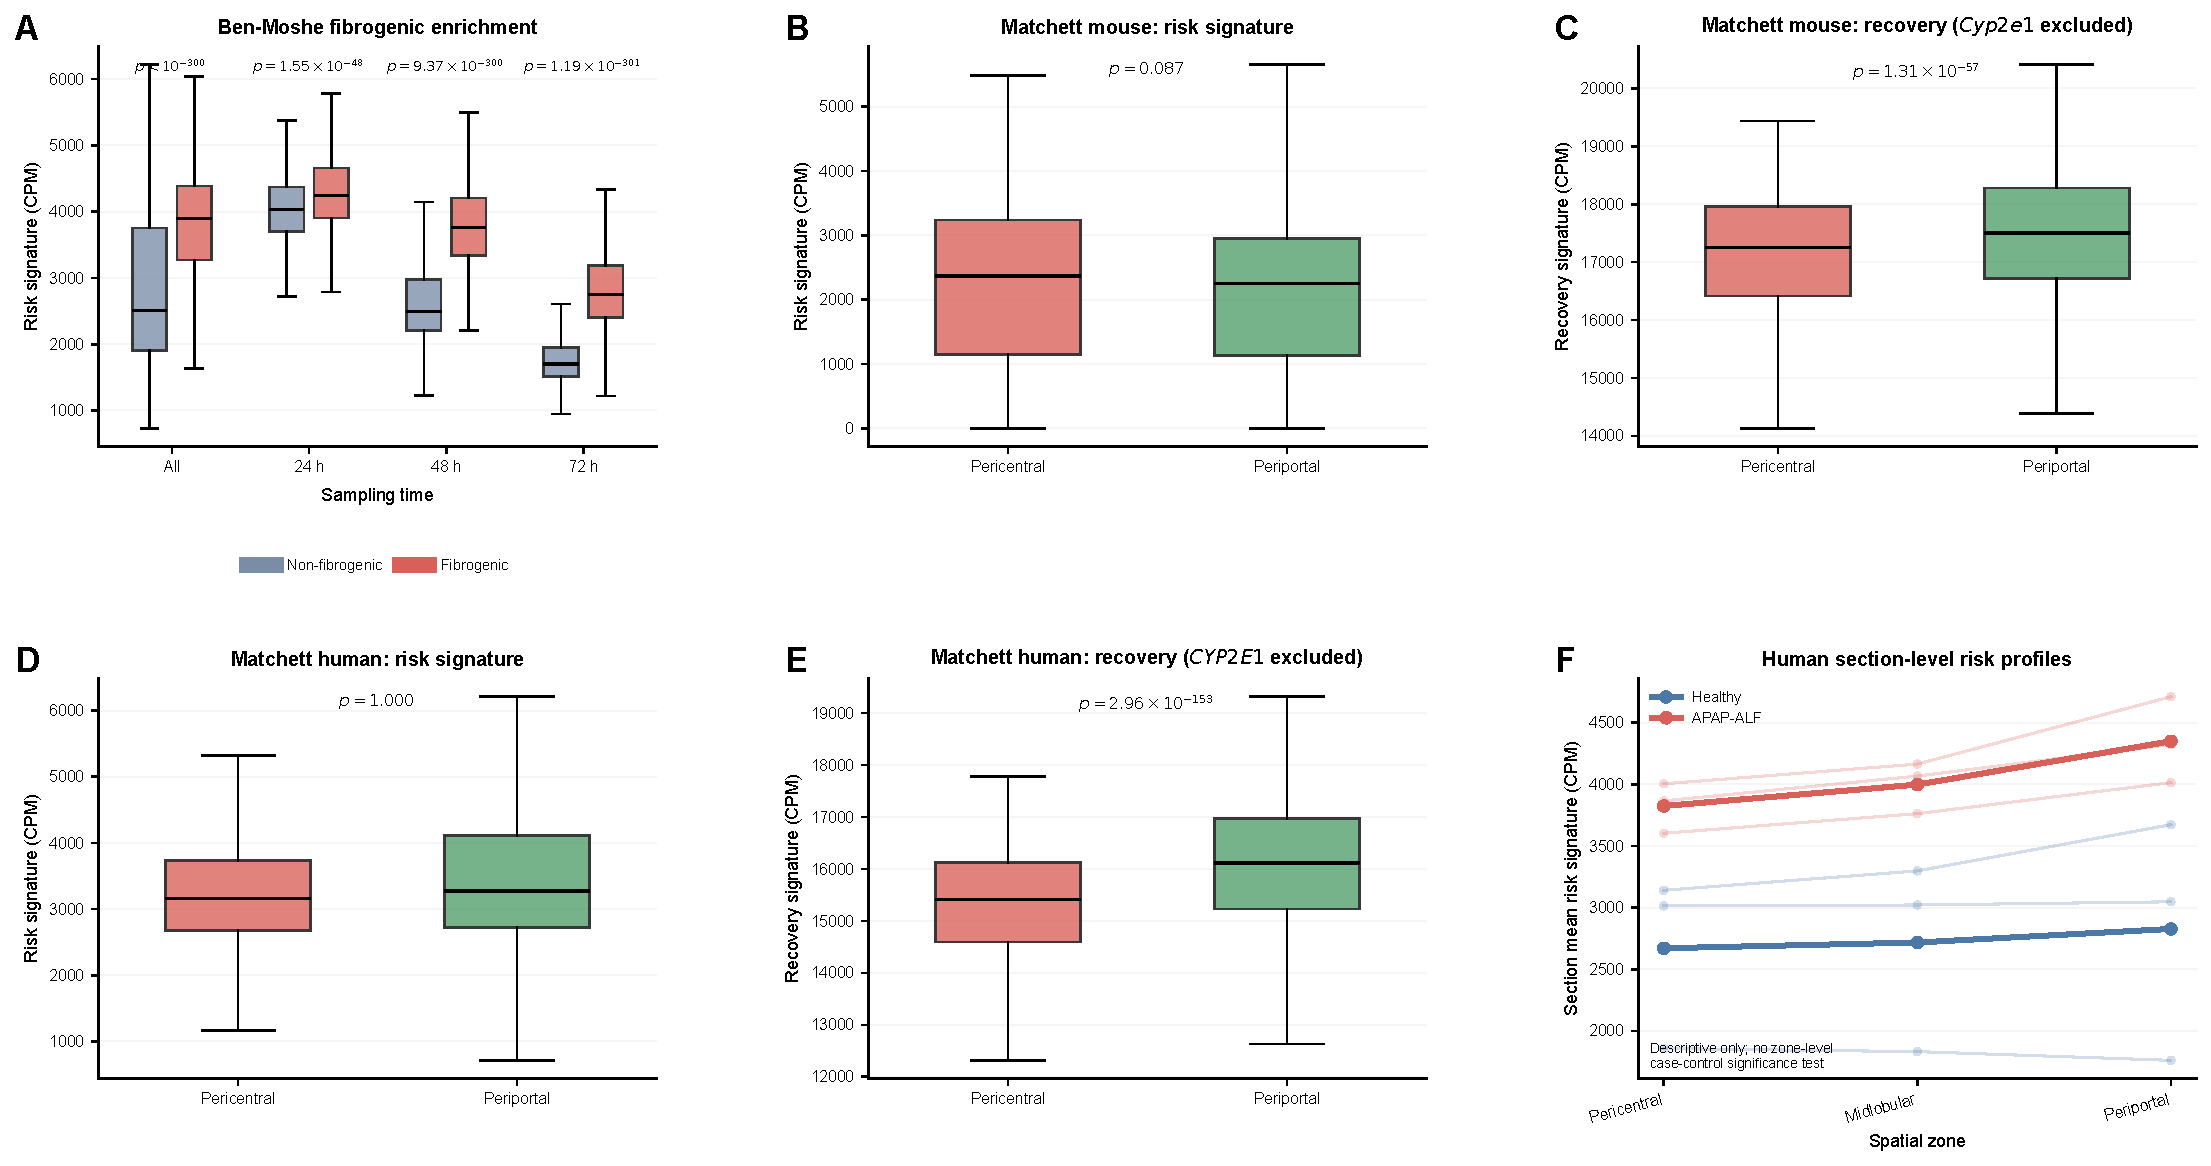
\includegraphics[width=0.64\textwidth,trim={708.000bp 286.872bp 0.000bp 0.000bp},clip]{figures/figure_S4.pdf}
\par\vspace{12pt}
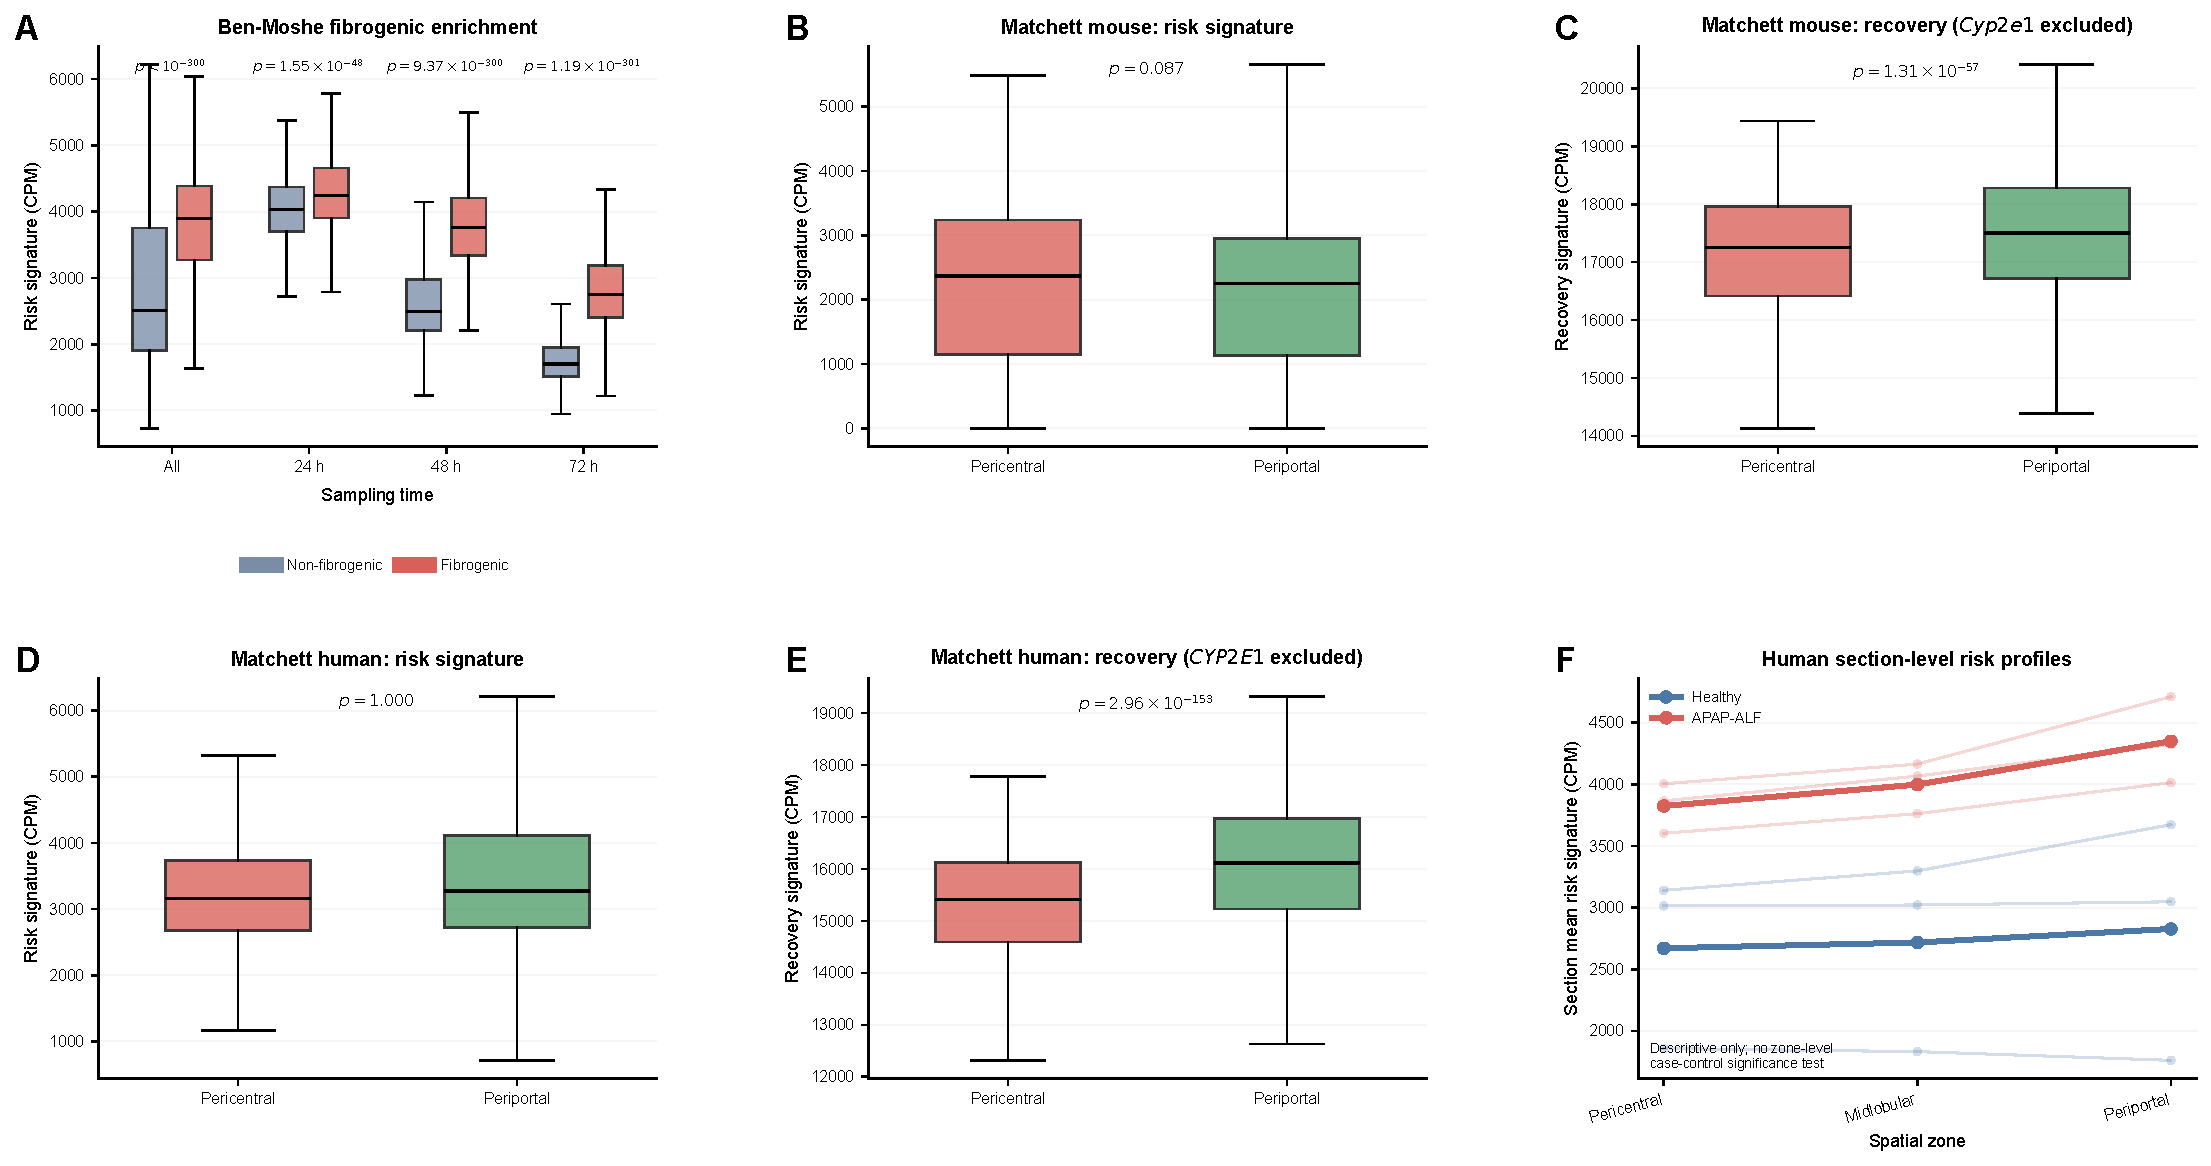
\includegraphics[width=0.64\textwidth,trim={0.000bp 0.000bp 706.415bp 285.000bp},clip]{figures/figure_S4.pdf}
\caption{\textbf{\FigSFourTitle{} (continued)} \textbf{(C)} \FigSFourC{} \textbf{(D)} \FigSFourD{}}
\end{figure}

\clearpage
\begin{figure}[H]
\centering
\ContinuedFloat
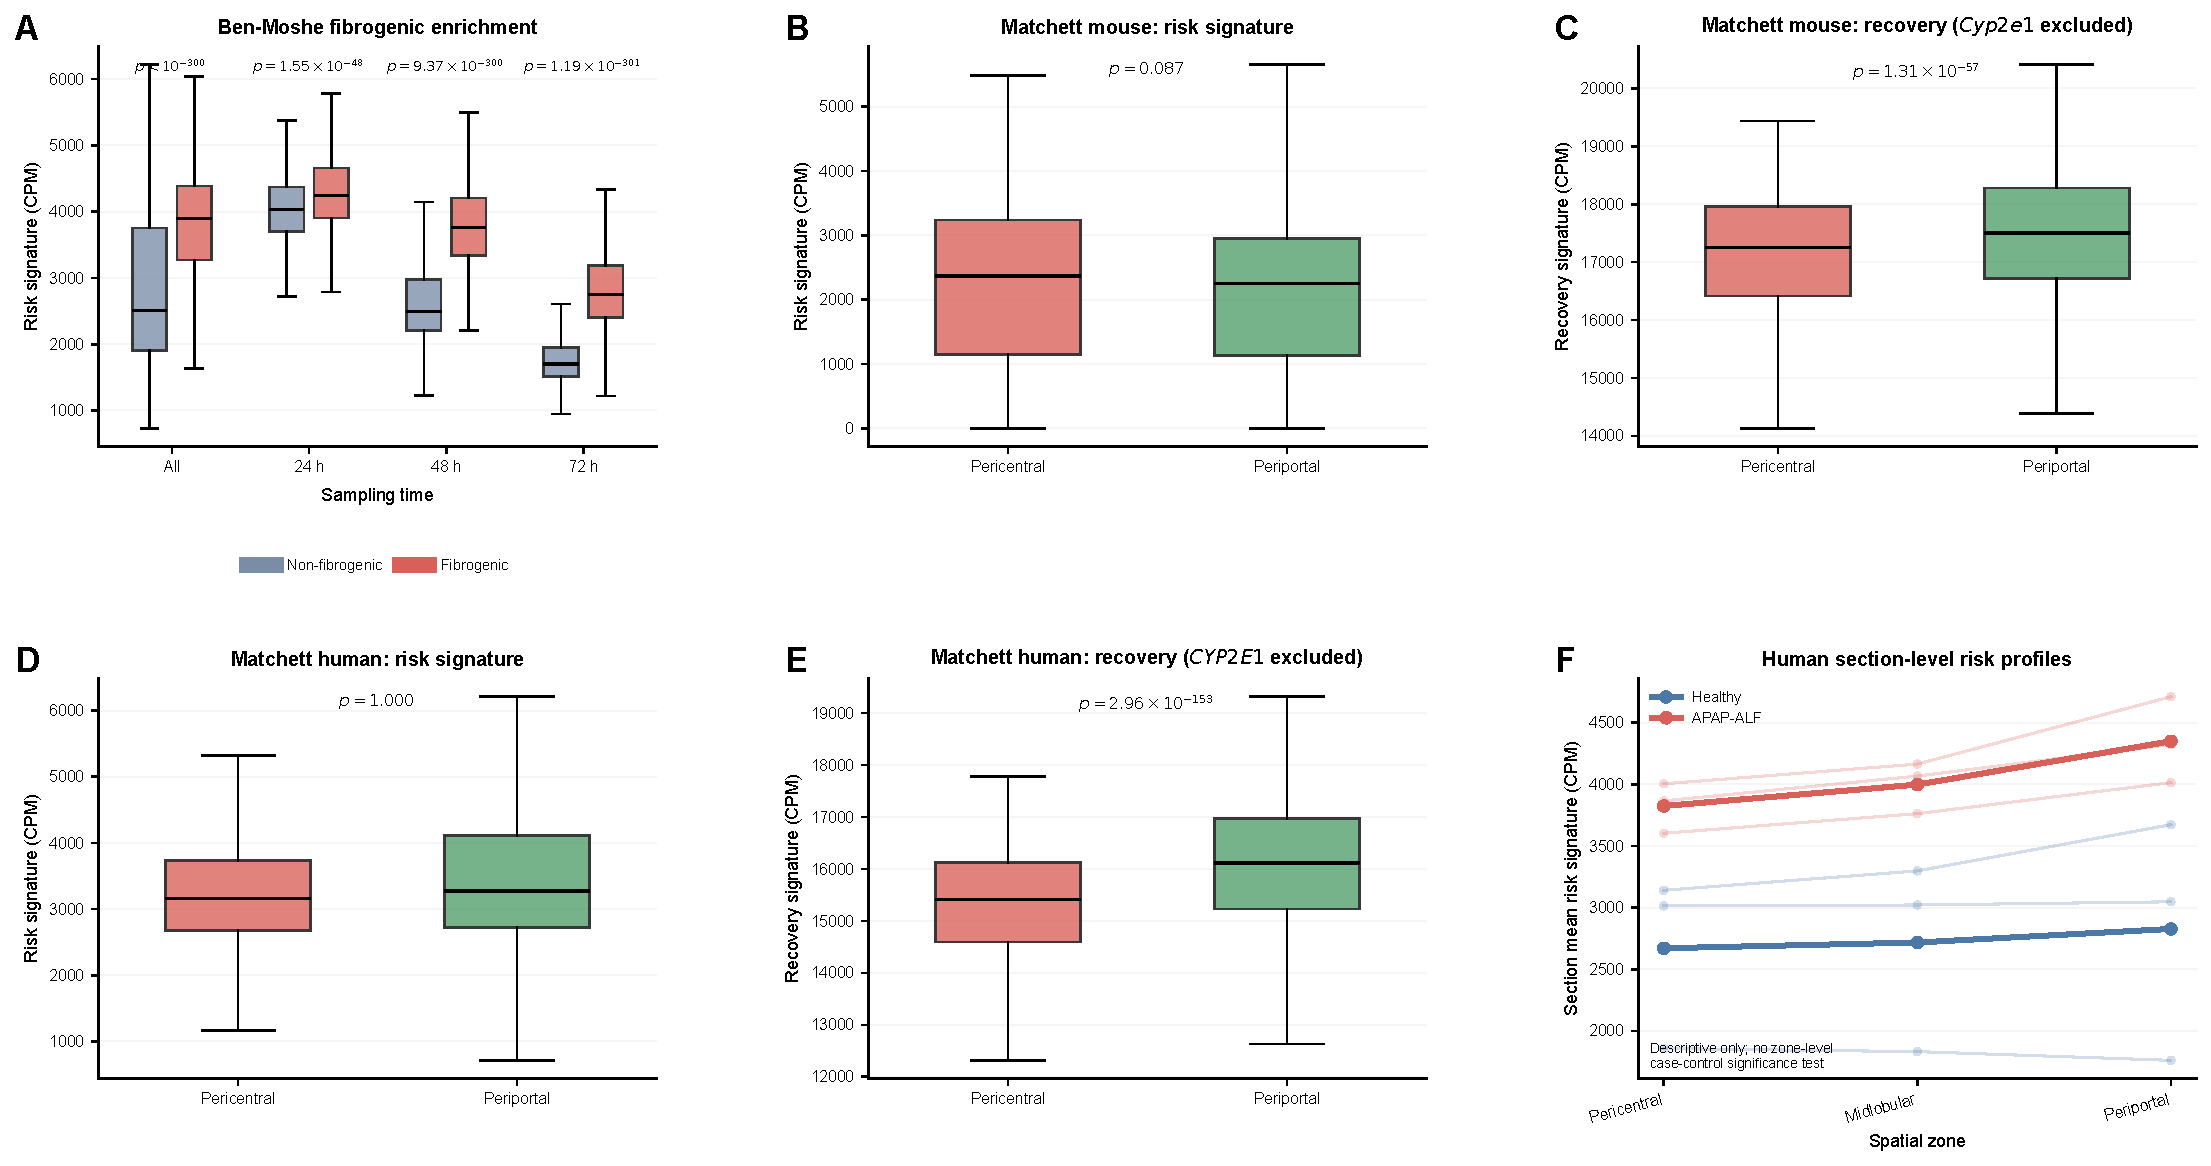
\includegraphics[width=0.64\textwidth,trim={356.000bp 0.000bp 354.415bp 285.000bp},clip]{figures/figure_S4.pdf}
\par\vspace{12pt}
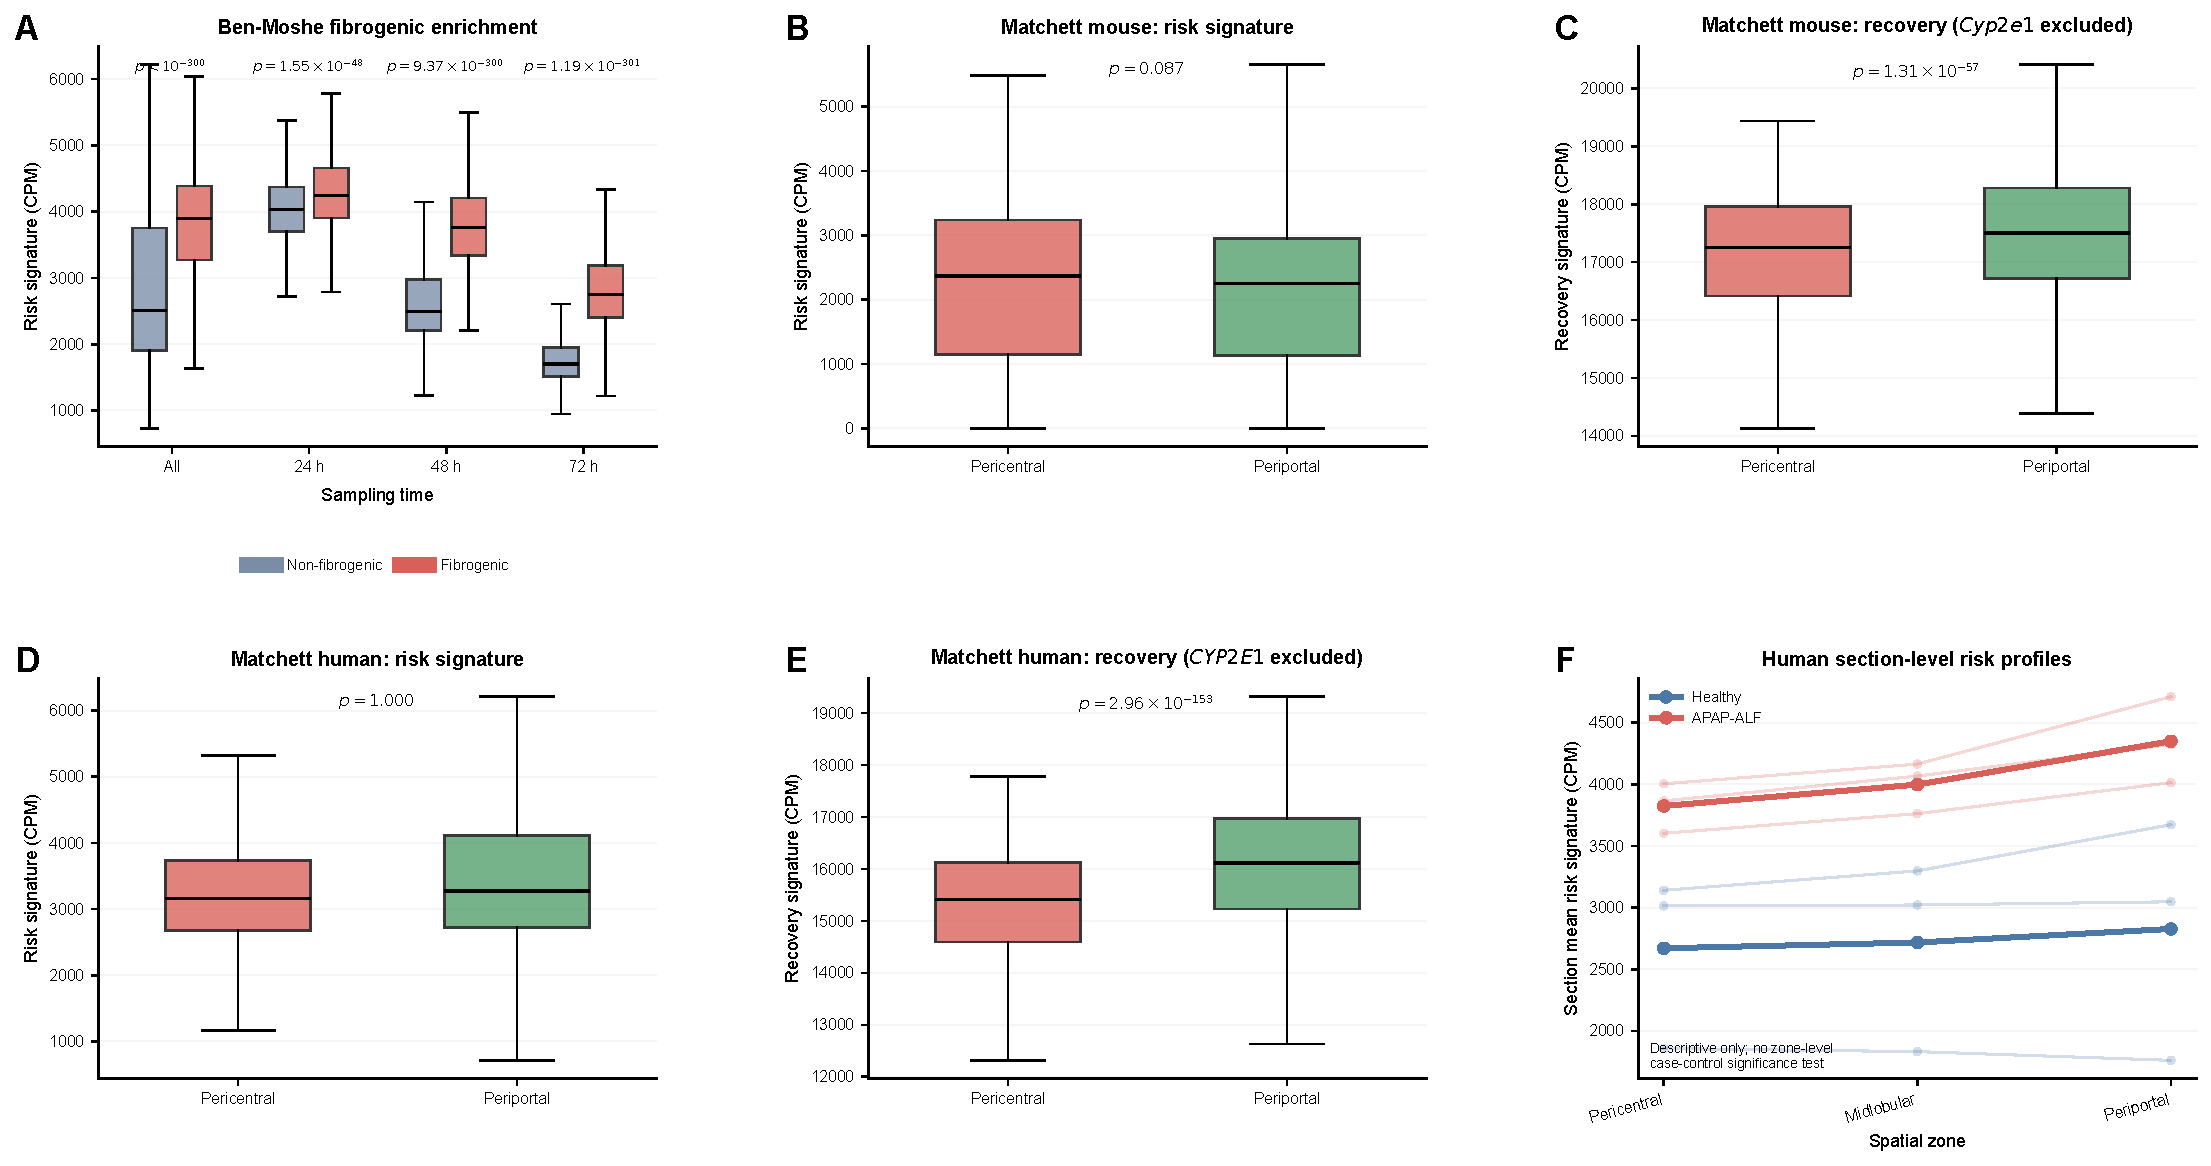
\includegraphics[width=0.64\textwidth,trim={708.000bp 0.000bp 0.000bp 285.000bp},clip]{figures/figure_S4.pdf}
\caption{\textbf{\FigSFourTitle{} (continued)} \textbf{(E)} \FigSFourE{} \textbf{(F)} \FigSFourF{} \FigSFourNotes{}}
\end{figure}

\clearpage
\begin{figure}[H]
\centering
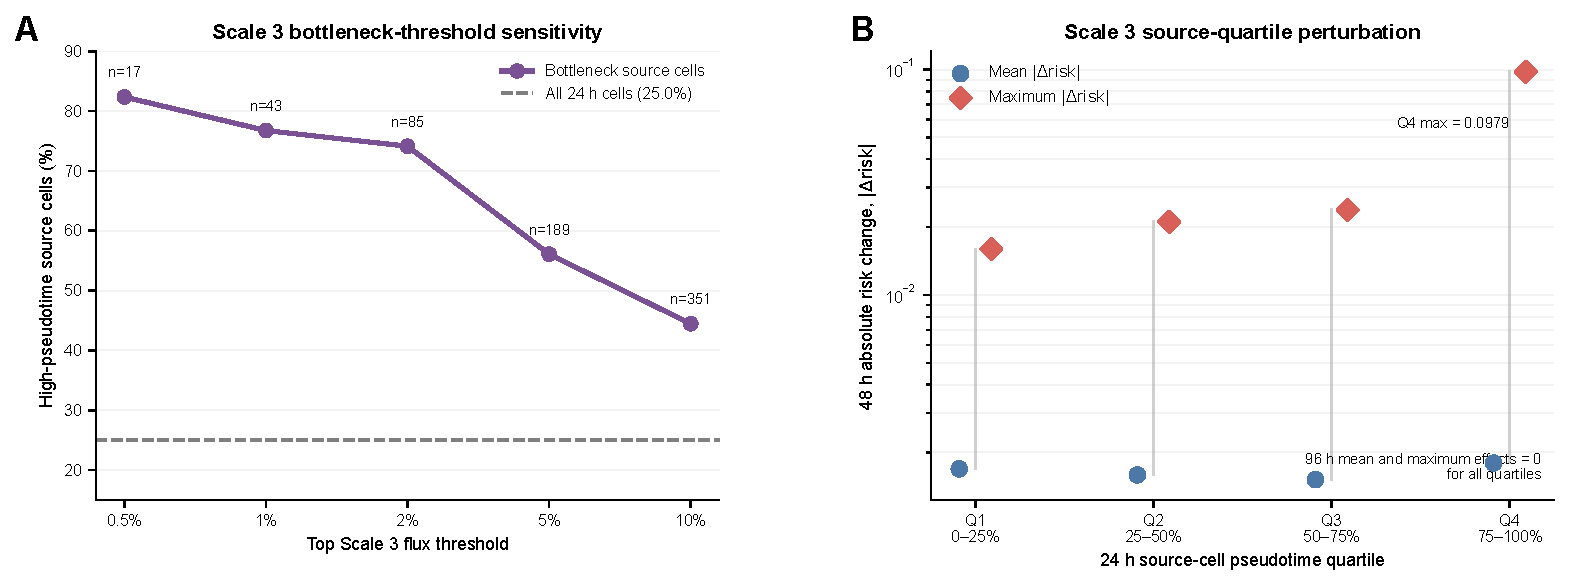
\includegraphics[width=0.68\textwidth,trim={0.000bp 0.000bp 377.120bp 0.000bp},clip]{figures/figure_S5.pdf}
\par\vspace{12pt}
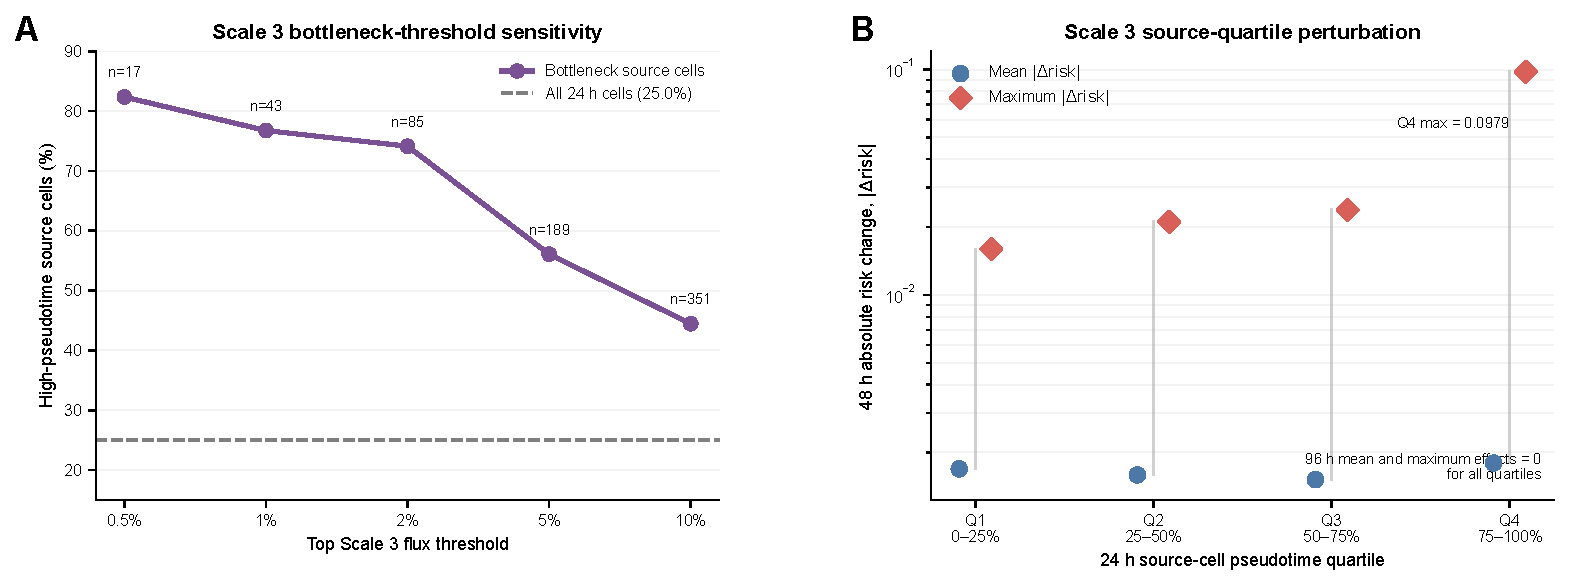
\includegraphics[width=0.68\textwidth,trim={377.000bp 0.000bp 0.000bp 0.000bp},clip]{figures/figure_S5.pdf}
\caption{\textbf{\FigSFiveTitle{}} \textbf{(A)} \FigSFiveA{} \textbf{(B)} \FigSFiveB{} \FigSFiveNotes{}}
\label{fig:S5}
\end{figure}
\clearpage
\section*{Table S1. Random Forest transition classifier performance and transition graph statistics across four temporal scales.}

\noindent Five-fold stratified cross-validation was used to evaluate each scale-specific classifier; CV AUROC is reported as mean \(\pm\) standard deviation across folds. OOB denotes out-of-bag accuracy. Raw RF probabilities below 0.30 were discarded before row normalization; when no target met this threshold, the 15 highest-probability targets were retained. Normalized probabilities below 0.001 were subsequently removed as a final sparsification step. Full-graph adjacency sparsity was calculated relative to the complete 6,582 \(\times\) 6,582 cell graph. Transition entropy is Shannon entropy of outgoing transition probabilities in nats, summarized across source cells as mean \(\pm\) standard deviation. RF--Gaussian Pearson r denotes the mean row-wise correlation between learned RF transitions and distance-only Gaussian transitions. Elapsed time is in hours; training-pair and edge counts are integers. RF, Random Forest; CV, cross-validation; AUROC, area under the receiver operating characteristic curve.

\phantomsection\label{tab:S1}
\noindent The four windows are 0--6, 6--24, 24--48, and 48--96~h. Sparsity is reported as a percentage of the complete cell graph, rather than of admissible pairs within each time window.

\Needspace{170pt}
\begingroup\small\setlength{\tabcolsep}{5pt}\renewcommand{\arraystretch}{1.23}
\noindent\begin{tabularx}{\textwidth}{>{\raggedright\arraybackslash}p{0.34\textwidth}*{4}{>{\raggedright\arraybackslash}X}}
\toprule
\textbf{Metric} & \textbf{Scale 1 (Acute Stress)} & \textbf{Scale 2 (Peak Injury)} & \textbf{Scale 3 (Fate Decision)} & \textbf{Scale 4 (Resolution)} \\ \midrule
Transition & 0~h \(\rightarrow\) 6~h & 6~h \(\rightarrow\) 24~h & 24~h \(\rightarrow\) 48~h & 48~h \(\rightarrow\) 96~h \\
Elapsed time (h) & 6 & 18 & 24 & 48 \\
Training pairs (n) & 153,045 & 18,855 & 46,935 & 40,950 \\
CV AUROC (mean \(\pm\) SD) & 0.9936 \(\pm\) 0.0002 & 0.9871 \(\pm\) 0.0011 & 0.9901 \(\pm\) 0.0004 & 0.9929 \(\pm\) 0.0009 \\
OOB accuracy & 0.9610 & 0.9490 & 0.9550 & 0.9650 \\
Retained edges (n) & 167,633 & 63,673 & 117,408 & 72,763 \\
Full-graph sparsity (\%) & 99.6130 & 99.8530 & 99.7290 & 99.8320 \\
Transition entropy (mean \(\pm\) SD, nats) & 3.81 \(\pm\) 0.26 & 4.88 \(\pm\) 0.42 & 4.58 \(\pm\) 0.39 & 4.24 \(\pm\) 0.43 \\
RF--Gaussian mean row Pearson r & 0.2460 & 0.1870 & 0.2490 & 0.4030 \\
\bottomrule
\end{tabularx}
\endgroup\par\medskip

\clearpage
\section*{Table S2. Internal performance of TrajRisk, comparator models, and component ablations.}
\phantomsection\label{tab:S2}
\noindent All final validation metrics use the same timepoint-stratified Walesky validation split of 1,318 cells, or the explicitly listed subset of that split. Binary labels are defined by normalized Monocle pseudotime > 0.10. Columns labeled high-risk refer to this elevated-pseudotime class, not observed future adverse outcomes. AUROC and AUPRC are dimensionless; AUPRC is average precision. Spearman rho measures association with continuous normalized pseudotime. The primary model was selected using validation AUROC; GNN ablations were selected on an inner development set. This checkpoint-selection asymmetry favors the primary model. The internal comparison is transductive: validation cells remain in the preconstructed graphs and their reference pseudotime values enter transition-pair features. All comparators share expression-derived features and targets. GNN, graph neural network; CI, confidence interval; pp, percentage points; RF, Random Forest; CV, cross-validation; AUROC, area under the receiver operating characteristic curve; AUPRC, area under the precision--recall curve.

\subsection*{Table S2A. Global baselines and ablations.}\phantomsection\label{tab:S2A}
\noindent AUROC 95\% CIs use 1,000 bootstrap resamples. Delta AUROC is 100 \(\times\) (TrajRisk AUROC minus comparator AUROC), in percentage points. One-sided paired bootstrap p values evaluate the directional comparison in favor of TrajRisk, using matched resamples of validation cells. An em dash denotes an unreported or inapplicable statistic; the seed's missing Spearman coefficient is not zero. The full-model delta is displayed as 0.00. B1 predicts continuous pseudotime from 30 scVI features using CV-tuned XGBoost. B2 propagates the scalar XGBoost seed through Gaussian matrices with damping 0.5. B3/\allowbreak{}A2 is the development-selected single-scale GNN. B4 is normalized expression-space distance from baseline controls. A1 substitutes Gaussian edge weights in the GNN. A3 uses scalar RF-matrix propagation with damping 0.5, jointly removing nonlinear aggregation and 31-dimensional node-feature integration. A4 omits the seed feature.

\Needspace{170pt}
\begingroup\small\setlength{\tabcolsep}{5pt}\renewcommand{\arraystretch}{1.23}
\noindent\begin{tabularx}{\textwidth}{>{\raggedright\arraybackslash}p{0.34\textwidth}*{5}{>{\raggedright\arraybackslash}X}}
\toprule
\textbf{Metric} & \textbf{TrajRisk (full)} & \textbf{Initial XGBoost seed (W6)} & \textbf{B1: XGBoost (CV-tuned)} & \textbf{B2: Gaussian propagation} & \textbf{B3/\allowbreak{}A2: Single-scale GNN (best)} \\ \midrule
Type & Proposed & Baseline & Baseline & Baseline & Baseline/\allowbreak{}Ablation \\
AUROC & 0.9071 & 0.8751 & 0.9582 & 0.8562 & 0.8502 \\
AUROC 95\% CI, lower & 0.8843 & 0.8535 & 0.9475 & 0.8329 & 0.8200 \\
AUROC 95\% CI, upper & 0.9310 & 0.8974 & 0.9682 & 0.8784 & 0.8824 \\
AUPRC & 0.7707 & 0.6745 & 0.8260 & 0.5026 & 0.6731 \\
Spearman rho & 0.5814 & --- & 0.7167 & 0.5426 & 0.4852 \\
TrajRisk minus comparator AUROC (pp) & 0.00 & 3.20 & -5.11 & 5.09 & 5.69 \\
One-sided paired bootstrap p & --- & --- & 1 & <0.001 & <0.001 \\
\bottomrule
\end{tabularx}
\endgroup\par\medskip
\Needspace{170pt}
\begingroup\small\setlength{\tabcolsep}{5pt}\renewcommand{\arraystretch}{1.23}
\noindent\begin{tabularx}{\textwidth}{>{\raggedright\arraybackslash}p{0.34\textwidth}*{4}{>{\raggedright\arraybackslash}X}}
\toprule
\textbf{Metric} & \textbf{B4: Expression distance} & \textbf{A1: Gaussian transitions} & \textbf{A3: RF matrix propagation} & \textbf{A4: No XGBoost seed} \\ \midrule
Type & Baseline & Ablation & Ablation & Ablation \\
AUROC & 0.8002 & 0.8257 & 0.8536 & 0.8281 \\
AUROC 95\% CI, lower & 0.7687 & 0.7937 & 0.8305 & 0.7958 \\
AUROC 95\% CI, upper & 0.8295 & 0.8591 & 0.8762 & 0.8618 \\
AUPRC & 0.4936 & 0.6519 & 0.5016 & 0.6587 \\
Spearman rho & 0.4541 & 0.4580 & 0.5538 & 0.4390 \\
TrajRisk minus comparator AUROC (pp) & 10.69 & 8.14 & 5.35 & 7.90 \\
One-sided paired bootstrap p & <0.001 & <0.001 & <0.001 & <0.001 \\
\bottomrule
\end{tabularx}
\endgroup\par\medskip

\clearpage
\subsection*{Table S2B. Single-scale GNN selection.}\phantomsection\label{tab:S2B}
\noindent Four one-scale GNNs were compared using development-set AUROC. Scale 4 was selected by that criterion; the held-out validation AUROC was subsequently reported. True/\allowbreak{}False indicates development-based selection, not selection on the validation results.

\Needspace{170pt}
\begingroup\small\setlength{\tabcolsep}{5pt}\renewcommand{\arraystretch}{1.23}
\noindent\begin{tabularx}{\textwidth}{>{\raggedright\arraybackslash}p{0.34\textwidth}*{4}{>{\raggedright\arraybackslash}X}}
\toprule
\textbf{Metric} & \textbf{Scale 1 (Acute Stress; 0~h\(\rightarrow\)6~h)} & \textbf{Scale 2 (Peak Injury; 6~h\(\rightarrow\)24~h)} & \textbf{Scale 3 (Fate Decision; 24~h\(\rightarrow\)48~h)} & \textbf{Scale 4 (Resolution; 48~h\(\rightarrow\)96~h)} \\ \midrule
Development AUROC & 0.8219 & 0.8427 & 0.8390 & 0.8432 \\
Validation AUROC & 0.8485 & 0.8374 & 0.8496 & 0.8502 \\
Selected by development AUROC & False & False & False & True \\
\bottomrule
\end{tabularx}
\endgroup\par\medskip

\clearpage
\subsection*{Table S2C. Within-timepoint and non-6~h validation performance.}\phantomsection\label{tab:S2C}
\noindent N is the number of validation cells in the indicated subset; N\_high\_risk is the number with normalized pseudotime > 0.10. Prevalence and random AUPRC equal N\_high\_risk/\allowbreak{}N and are recorded as fractions. Non-6~h excludes all 6~h cells. The 24, 48, and 96~h groups contain 209, 182, and 162 validation cells, respectively. No additional hypothesis test is reported for these within-timepoint comparisons.

\Needspace{170pt}
\par\medskip\noindent\textbf{Non-6~h}\par
\begingroup\small\setlength{\tabcolsep}{5pt}\renewcommand{\arraystretch}{1.23}
\noindent\begin{tabularx}{\textwidth}{>{\raggedright\arraybackslash}p{0.34\textwidth}*{3}{>{\raggedright\arraybackslash}X}}
\toprule
\textbf{Metric} & \textbf{TrajRisk} & \textbf{Seeder (W6)} & \textbf{B1 XGBoost} \\ \midrule
N & 1,234 & 1,234 & 1,234 \\
High-risk cells (n) & 130 & 130 & 130 \\
High-risk prevalence & 0.1053 & 0.1053 & 0.1053 \\
AUROC & 0.8561 & 0.7964 & 0.9326 \\
AUPRC & 0.4641 & 0.2482 & 0.4920 \\
Random AUPRC & 0.1053 & 0.1053 & 0.1053 \\
\bottomrule
\end{tabularx}
\endgroup\par\medskip
\Needspace{170pt}
\par\medskip\noindent\textbf{24~h}\par
\begingroup\small\setlength{\tabcolsep}{5pt}\renewcommand{\arraystretch}{1.23}
\noindent\begin{tabularx}{\textwidth}{>{\raggedright\arraybackslash}p{0.34\textwidth}*{3}{>{\raggedright\arraybackslash}X}}
\toprule
\textbf{Metric} & \textbf{TrajRisk} & \textbf{Seeder (W6)} & \textbf{B1 XGBoost} \\ \midrule
N & 209 & 209 & 209 \\
High-risk cells (n) & 36 & 36 & 36 \\
High-risk prevalence & 0.1722 & 0.1722 & 0.1722 \\
AUROC & 0.7399 & 0.6911 & 0.8009 \\
AUPRC & 0.4983 & 0.3224 & 0.3793 \\
Random AUPRC & 0.1722 & 0.1722 & 0.1722 \\
\bottomrule
\end{tabularx}
\endgroup\par\medskip
\Needspace{170pt}
\par\medskip\noindent\textbf{48~h}\par
\begingroup\small\setlength{\tabcolsep}{5pt}\renewcommand{\arraystretch}{1.23}
\noindent\begin{tabularx}{\textwidth}{>{\raggedright\arraybackslash}p{0.34\textwidth}*{3}{>{\raggedright\arraybackslash}X}}
\toprule
\textbf{Metric} & \textbf{TrajRisk} & \textbf{Seeder (W6)} & \textbf{B1 XGBoost} \\ \midrule
N & 182 & 182 & 182 \\
High-risk cells (n) & 41 & 41 & 41 \\
High-risk prevalence & 0.2253 & 0.2253 & 0.2253 \\
AUROC & 0.6937 & 0.4634 & 0.8677 \\
AUPRC & 0.4627 & 0.2000 & 0.5970 \\
Random AUPRC & 0.2253 & 0.2253 & 0.2253 \\
\bottomrule
\end{tabularx}
\endgroup\par\medskip
\Needspace{170pt}
\par\medskip\noindent\textbf{96~h}\par
\begingroup\small\setlength{\tabcolsep}{5pt}\renewcommand{\arraystretch}{1.23}
\noindent\begin{tabularx}{\textwidth}{>{\raggedright\arraybackslash}p{0.34\textwidth}*{3}{>{\raggedright\arraybackslash}X}}
\toprule
\textbf{Metric} & \textbf{TrajRisk} & \textbf{Seeder (W6)} & \textbf{B1 XGBoost} \\ \midrule
N & 162 & 162 & 162 \\
High-risk cells (n) & 50 & 50 & 50 \\
High-risk prevalence & 0.3086 & 0.3086 & 0.3086 \\
AUROC & 0.7729 & 0.4300 & 0.8730 \\
AUPRC & 0.5813 & 0.2725 & 0.6922 \\
Random AUPRC & 0.3086 & 0.3086 & 0.3086 \\
\bottomrule
\end{tabularx}
\endgroup\par\medskip

\clearpage
\section*{Table S3. External mouse-cohort discrimination and association with \textit{Cdkn1a} expression.}
\phantomsection\label{tab:S3}
\noindent The Walesky-trained mouse model and comparators were transferred without refitting. \SelfOnly{} inference uses the learned self pathway without incoming reference edges. Reference-KNN inference adds the 15 nearest Walesky reference neighbors in the integrated 30-dimensional scVI space. AUROC CIs use 1,000 bootstrap resamples. Random AUPRC equals the positive-class prevalence. Reported fractions and model scores are dimensionless. APAP, acetaminophen; KNN, k-nearest neighbors; CI, confidence interval; AUROC, area under the receiver operating characteristic curve; AUPRC, area under the precision--recall curve.

\subsection*{Table S3A. External APAP-versus-control classification.}\phantomsection\label{tab:S3A}
\noindent APAP treatment is the positive class. N includes all evaluated cells, including controls, in each cohort: Ben-Moshe, 2,770; Umbaugh 2~h, 21,409; Umbaugh 48/\allowbreak{}72~h, 5,306. N\_positive counts APAP-treated cells. The Ben-Moshe label identifies the APAP sampling times and does not exclude its baseline controls. These tests distinguish treatment condition, rather than observed future cell fate. Pairwise significance tests between methods are not reported for these comparisons.

\Needspace{170pt}
\par\medskip\noindent\textbf{Ben-Moshe 48/\allowbreak{}72~h --- APAP vs Control}\par
\begingroup\small\setlength{\tabcolsep}{5pt}\renewcommand{\arraystretch}{1.23}
\noindent\begin{tabularx}{\textwidth}{>{\raggedright\arraybackslash}p{0.34\textwidth}*{4}{>{\raggedright\arraybackslash}X}}
\toprule
\textbf{Metric} & \textbf{TrajRisk Reference-KNN} & \textbf{TrajRisk \SelfOnly{}} & \textbf{Initial XGBoost seed} & \textbf{Expression-only XGBoost} \\ \midrule
N & 2,770 & 2,770 & 2,770 & 2,770 \\
Positive cells (n) & 771 & 771 & 771 & 771 \\
Prevalence & 0.2783 & 0.2783 & 0.2783 & 0.2783 \\
AUROC & 0.7197 & 0.8069 & 0.8541 & 0.8544 \\
AUROC 95\% CI, lower & 0.6973 & 0.7869 & 0.8381 & 0.8387 \\
AUROC 95\% CI, upper & 0.7418 & 0.8261 & 0.8691 & 0.8706 \\
AUPRC & 0.5652 & 0.7103 & 0.7371 & 0.7534 \\
Random AUPRC & 0.2783 & 0.2783 & 0.2783 & 0.2783 \\
\bottomrule
\end{tabularx}
\endgroup\par\medskip
\Needspace{170pt}
\par\medskip\noindent\textbf{Umbaugh 2~h --- APAP vs Control}\par
\begingroup\small\setlength{\tabcolsep}{5pt}\renewcommand{\arraystretch}{1.23}
\noindent\begin{tabularx}{\textwidth}{>{\raggedright\arraybackslash}p{0.34\textwidth}*{4}{>{\raggedright\arraybackslash}X}}
\toprule
\textbf{Metric} & \textbf{TrajRisk Reference-KNN} & \textbf{TrajRisk \SelfOnly{}} & \textbf{Initial XGBoost seed} & \textbf{Expression-only XGBoost} \\ \midrule
N & 21,409 & 21,409 & 21,409 & 21,409 \\
Positive cells (n) & 13,502 & 13,502 & 13,502 & 13,502 \\
Prevalence & 0.6307 & 0.6307 & 0.6307 & 0.6307 \\
AUROC & 0.6524 & 0.6087 & 0.6465 & 0.6422 \\
AUROC 95\% CI, lower & 0.6451 & 0.6012 & 0.6393 & 0.6349 \\
AUROC 95\% CI, upper & 0.6600 & 0.6166 & 0.6541 & 0.6497 \\
AUPRC & 0.7944 & 0.7566 & 0.7902 & 0.7677 \\
Random AUPRC & 0.6307 & 0.6307 & 0.6307 & 0.6307 \\
\bottomrule
\end{tabularx}
\endgroup\par\medskip
\Needspace{170pt}
\par\medskip\noindent\textbf{Umbaugh 48/\allowbreak{}72~h --- APAP vs Control}\par
\begingroup\small\setlength{\tabcolsep}{5pt}\renewcommand{\arraystretch}{1.23}
\noindent\begin{tabularx}{\textwidth}{>{\raggedright\arraybackslash}p{0.34\textwidth}*{4}{>{\raggedright\arraybackslash}X}}
\toprule
\textbf{Metric} & \textbf{TrajRisk Reference-KNN} & \textbf{TrajRisk \SelfOnly{}} & \textbf{Initial XGBoost seed} & \textbf{Expression-only XGBoost} \\ \midrule
N & 5,306 & 5,306 & 5,306 & 5,306 \\
Positive cells (n) & 2,978 & 2,978 & 2,978 & 2,978 \\
Prevalence & 0.5613 & 0.5613 & 0.5613 & 0.5613 \\
AUROC & 0.7939 & 0.8958 & 0.9330 & 0.9423 \\
AUROC 95\% CI, lower & 0.7824 & 0.8869 & 0.9263 & 0.9362 \\
AUROC 95\% CI, upper & 0.8067 & 0.9047 & 0.9396 & 0.9480 \\
AUPRC & 0.8192 & 0.9047 & 0.9306 & 0.9510 \\
Random AUPRC & 0.5613 & 0.5613 & 0.5613 & 0.5613 \\
\bottomrule
\end{tabularx}
\endgroup\par\medskip

\clearpage
\subsection*{Table S3B. \textit{Cdkn1a} expression association in 5,306 Umbaugh 48/\allowbreak{}72~h hepatocytes.}\phantomsection\label{tab:S3B}
\noindent The detection task compares cells with \textit{Cdkn1a} expression > 0 against those with zero expression; the positive-class prevalence is 0.3407. Spearman rho and its two-sided nominal p value use continuous \textit{Cdkn1a} expression across all 5,306 cells. Group means summarize model scores. One-sided Mann--Whitney U tests evaluate greater scores in \textit{Cdkn1a}-expressing cells. Detection of \textit{Cdkn1a} transcript is the operational label; it does not directly measure p21 protein.

\Needspace{170pt}
\begingroup\small\setlength{\tabcolsep}{5pt}\renewcommand{\arraystretch}{1.23}
\noindent\begin{tabularx}{\textwidth}{>{\raggedright\arraybackslash}p{0.34\textwidth}*{4}{>{\raggedright\arraybackslash}X}}
\toprule
\textbf{Metric} & \textbf{TrajRisk Reference-KNN} & \textbf{TrajRisk \SelfOnly{}} & \textbf{Initial XGBoost seed} & \textbf{Expression-only XGBoost} \\ \midrule
\textit{Cdkn1a} detection AUROC & 0.6922 & 0.7372 & 0.7608 & 0.7567 \\
AUROC 95\% CI, lower & 0.6782 & 0.7240 & 0.7484 & 0.7441 \\
AUROC 95\% CI, upper & 0.7075 & 0.7517 & 0.7742 & 0.7705 \\
\textit{Cdkn1a} detection AUPRC & 0.4790 & 0.5127 & 0.5588 & 0.5841 \\
Random AUPRC & 0.3407 & 0.3407 & 0.3407 & 0.3407 \\
Continuous \textit{Cdkn1a} Spearman rho & 0.3134 & 0.3822 & 0.4179 & 0.4037 \\
Spearman p & \(2.744\times10^{-121}\) & \(3.838\times10^{-184}\) & \(2.254\times10^{-223}\) & \(3.885\times10^{-207}\) \\
Mean score, \textit{Cdkn1a}-expressing & 0.3036 & 0.3689 & 0.8973 & 0.5410 \\
Mean score, \textit{Cdkn1a}-zero & 0.1686 & 0.1826 & 0.5359 & 0.3056 \\
One-sided U-test p (expressed > zero) & \(3.701\times10^{-117}\) & \(2.621\times10^{-177}\) & \(9.135\times10^{-214}\) & \(3.223\times10^{-207}\) \\
\bottomrule
\end{tabularx}
\endgroup\par\medskip

\clearpage
\section*{Table S4. Cross-species integration, human donor-level validation, and signature concordance.}
\phantomsection\label{tab:S4}
\noindent The shared scVI representation contains 6,582 Walesky mouse hepatocytes and 49,984 Matchett human hepatocyte nuclei on 13,122 retained unique mouse--human gene-symbol pairs, with 30 latent dimensions. The cross-species GNN and seeder were trained on mouse cells in these shared coordinates; human donor labels were not used for model training. \SelfOnly{} is the primary human analysis and Reference-KNN is a sensitivity analysis. APAP-ALF, acetaminophen-induced acute liver failure; ASW, average silhouette width; GNN, graph neural network; KNN, k-nearest neighbors; AUROC, area under the receiver operating characteristic curve.

\subsection*{Table S4A. Cross-species integration characteristics.}\phantomsection\label{tab:S4A}
\noindent Species and condition ASW were independently calculated on the same 10,000-observation subsample of the joint 30-dimensional latent space. Their values (0.0346643 and 0.0346610, respectively) both round to 0.0347; the matching displayed values are not duplicate measurements. Low ASW describes label mixing and does not alone establish preservation of biological condition structure. The validation AUROC of 0.9219 is for held-out Walesky mouse cells in the cross-species coordinate system, rather than human donors. Cell/\allowbreak{}nucleus and retained gene-symbol-pair counts are integers; ASW and AUROC are dimensionless.

\begingroup\small\renewcommand{\arraystretch}{1.25}
\noindent\begin{tabularx}{\textwidth}{>{\raggedright\arraybackslash}p{0.38\textwidth}>{\raggedright\arraybackslash}p{0.12\textwidth}X}
\toprule Metric & Value & Note \\ \midrule
Retained unique mouse--human gene-symbol pairs & 13,122 & Mappings present in both Walesky and Matchett expression matrices \\
Walesky mouse hepatocytes & 6,582 & Mouse training/\allowbreak{}reference cells \\
Matchett human hepatocyte nuclei & 49,984 & 10 APAP-ALF donors + 9 healthy donors \\
Joint cross-species cells/\allowbreak{}nuclei & 56,566 & Combined cross-species scVI dataset \\
ASW (species labels) & 0.0347 & Computed in 30-dimensional cross-species scVI latent space \\
ASW (condition labels) & 0.0347 & Cross-species latent-space diagnostic \\
Cross-species TrajRisk validation AUROC & 0.9219 & Held-out Walesky validation set in cross-species coordinate system \\
\bottomrule\end{tabularx}\endgroup\par\medskip

\clearpage
\subsection*{Table S4B. Human donor-level condition discrimination.}\phantomsection\label{tab:S4B}
\noindent Nucleus scores are averaged within each donor before analysis. Condition means are unweighted means of donor values. The primary cohort contains 10 APAP-ALF and 9 healthy donors. The sensitivity cohort excludes four APAP-ALF donors with fewer than 300 retained hepatocyte nuclei, leaving 6 APAP-ALF and 9 healthy donors. One-sided Mann--Whitney U tests evaluate APAP-ALF > healthy. AUROC uses APAP-ALF as the positive class and preserves the recorded score direction. The raw risk signature averages log-normalized expression of mapped risk genes; the net signature subtracts the recovery signature. No direction reversal was applied to improve signature AUROC.

\Needspace{170pt}
\par\medskip\noindent\textbf{Primary cohort}\par
\begingroup\small\setlength{\tabcolsep}{5pt}\renewcommand{\arraystretch}{1.23}
\noindent\begin{tabularx}{\textwidth}{>{\raggedright\arraybackslash}p{0.34\textwidth}*{4}{>{\raggedright\arraybackslash}X}}
\toprule
\textbf{Metric} & \textbf{TrajRisk \SelfOnly{}} & \textbf{TrajRisk Reference-KNN} & \textbf{Net orthologous gene signature} & \textbf{Raw risk gene signature} \\ \midrule
APAP-ALF donors (n) & 10 & 10 & 10 & 10 \\
Healthy donors (n) & 9 & 9 & 9 & 9 \\
APAP-ALF donor mean & 0.2051 & 0.2144 & 0.1328 & 0.3585 \\
Healthy donor mean & 0.1088 & 0.1224 & 0.0942 & 0.4380 \\
One-sided Mann--Whitney p & 0.0064 & 0.0080 & 0.1352 & 0.9995 \\
Donor-level AUROC & 0.8444 & 0.8333 & 0.6556 & 0.0556 \\
\bottomrule
\end{tabularx}
\endgroup\par\medskip
\Needspace{170pt}
\par\medskip\noindent\textbf{Sensitivity cohort (\(\geq\)300 hepatocyte nuclei per ALF donor)}\par
\begingroup\small\setlength{\tabcolsep}{5pt}\renewcommand{\arraystretch}{1.23}
\noindent\begin{tabularx}{\textwidth}{>{\raggedright\arraybackslash}p{0.34\textwidth}*{4}{>{\raggedright\arraybackslash}X}}
\toprule
\textbf{Metric} & \textbf{TrajRisk \SelfOnly{}} & \textbf{TrajRisk Reference-KNN} & \textbf{Net orthologous gene signature} & \textbf{Raw risk gene signature} \\ \midrule
APAP-ALF donors (n) & 6 & 6 & 6 & 6 \\
Healthy donors (n) & 9 & 9 & 9 & 9 \\
APAP-ALF donor mean & 0.1421 & 0.1494 & 0.0921 & 0.3641 \\
Healthy donor mean & 0.1088 & 0.1224 & 0.0942 & 0.4380 \\
One-sided Mann--Whitney p & 0.0248 & 0.0332 & 0.5227 & 0.9986 \\
Donor-level AUROC & 0.8148 & 0.7963 & 0.5000 & 0.0741 \\
\bottomrule
\end{tabularx}
\endgroup\par\medskip

\clearpage
\subsection*{Table S4C. Reference-KNN score and net-signature concordance.}\phantomsection\label{tab:S4C}
\noindent Spearman rho and two-sided nominal p values compare donor-mean Reference-KNN TrajRisk scores with donor-mean net signature scores across 19 primary-cohort or 15 sensitivity-cohort donors. This table concerns the Reference-KNN variant, not the primary \SelfOnly{} score. Both summaries use the same donor expression data and the association is not independent biological replication.

\Needspace{170pt}
\begingroup\small\setlength{\tabcolsep}{5pt}\renewcommand{\arraystretch}{1.23}
\noindent\begin{tabularx}{\textwidth}{>{\raggedright\arraybackslash}p{0.34\textwidth}*{2}{>{\raggedright\arraybackslash}X}}
\toprule
\textbf{Metric} & \textbf{Primary cohort} & \textbf{Sensitivity cohort (\(\geq\)300 hepatocyte nuclei per ALF donor)} \\ \midrule
N donors & 19 & 15 \\
Comparison & TrajRisk Reference-KNN vs net gene signature & TrajRisk Reference-KNN vs net gene signature \\
Spearman rho & 0.8333 & 0.6679 \\
Spearman p & \(9.401\times10^{-6}\) & 0.0065 \\
\bottomrule
\end{tabularx}
\endgroup\par\medskip

\clearpage
\section*{Table S5. Spatial risk- and recovery-signature analyses in mouse and human liver.}
\phantomsection\label{tab:S5}
\noindent Spatial scores are mean counts per million (CPM) across signature genes after spot-level library-size normalization. These are gene-signature scores, rather than spatially projected GNN score predictions. The risk signature contains 50 genes. Matchett pericentral spots have \textit{Cyp2e1}/\allowbreak{}\textit{CYP2E1} CPM at or above the within-section 75th percentile; periportal spots are at or below the 25th percentile; remaining spots are midlobular. Percentiles use linear interpolation, and all boundary ties enter the corresponding zone. \textit{Cyp2e1}/\allowbreak{}\textit{CYP2E1} is excluded from Matchett recovery and net scoring, leaving 49 recovery genes, to avoid circularity with zonation. P values are nominal and spot-pooled tests do not use donors as independent inferential units. APAP-ALF, acetaminophen-induced acute liver failure; CPM, counts per million; GNN, graph neural network; SD, standard deviation.

\subsection*{Table S5A. Ben-Moshe fibrogenic risk-signature enrichment.}\phantomsection\label{tab:S5A}
\noindent Deposited fibrogenic annotations define the comparison. Six sections from two mice per timepoint contain 17,370 spots: 3,395 fibrogenic and 13,975 non-fibrogenic. Counts, medians, and means are listed for pooled data and for each timepoint. The one-sided Mann--Whitney U alternative is fibrogenic > non-fibrogenic. The pooled p value recorded as 0.0 is displayed as \(<10^{-300}\), consistent with the manuscript's reporting convention.

\Needspace{170pt}
\begingroup\small\setlength{\tabcolsep}{5pt}\renewcommand{\arraystretch}{1.23}
\noindent\begin{tabularx}{\textwidth}{>{\raggedright\arraybackslash}p{0.34\textwidth}*{4}{>{\raggedright\arraybackslash}X}}
\toprule
\textbf{Metric} & \textbf{All timepoints} & \textbf{24~h} & \textbf{48~h} & \textbf{72~h} \\ \midrule
Fibrogenic spots (n) & 3,395 & 1,677 & 962 & 756 \\
Non-fibrogenic spots (n) & 13,975 & 4,086 & 5,460 & 4,429 \\
Median risk fibrogenic & 3,892.6172 & 4,245.2830 & 3,762.8191 & 2,754.4259 \\
Median risk nonfibrogenic & 2,511.9233 & 4,028.7769 & 2,494.7361 & 1,700 \\
Mean risk fibrogenic & 3,814.0292 & 4,281.0629 & 3,793.6296 & 2,803.9879 \\
Mean risk nonfibrogenic & 2,798.2342 & 4,040.7368 & 2,693.7506 & 1,780.7618 \\
Mann Whitney U & 36,252,944.5000 & 4,263,327.5000 & 4,587,397 & 3,085,611.5000 \\
One-sided U-test p (fibrogenic > other) & \(<10^{-300}\) & \(1.551\times10^{-48}\) & \(9.367\times10^{-300}\) & \(1.191\times10^{-301}\) \\
\bottomrule
\end{tabularx}
\endgroup\par\medskip

\clearpage
\subsection*{Table S5B. Matchett mouse zonation and \textit{Cyp2e1} association.}\phantomsection\label{tab:S5B}
\noindent Eleven sections contribute 6,335 pericentral and 6,334 periportal spots. One-sided Mann--Whitney U alternatives are pericentral > periportal for the risk signature and pericentral < periportal for the corrected recovery signature. Group summaries are medians of pooled spot scores. Statistic is U for these comparisons and Spearman rho for the \textit{Cyp2e1} association. Empty zonation-summary fields in the correlation record are inapplicable. The correlation p value recorded as 0.0 is displayed as numerical underflow.

\Needspace{170pt}
\begingroup\small\setlength{\tabcolsep}{5pt}\renewcommand{\arraystretch}{1.23}
\noindent\begin{tabularx}{\textwidth}{>{\raggedright\arraybackslash}p{0.34\textwidth}*{3}{>{\raggedright\arraybackslash}X}}
\toprule
\textbf{Metric} & \textbf{Risk signature: pericentral > periportal} & \textbf{Recovery signature excluding \textit{Cyp2e1}: pericentral < periportal} & \textbf{\textit{Cyp2e1} vs risk signature Spearman correlation} \\ \midrule
Dataset & Matchett mouse Visium & Matchett mouse Visium & Matchett mouse Visium \\
Pericentral spots (n) & 6,335 & 6,335 & --- \\
Periportal spots (n) & 6,334 & 6,334 & --- \\
Pericentral median (CPM) & 2,369.9732 & 17,248.7405 & --- \\
Periportal median (CPM) & 2,253.6461 & 17,505.4070 & --- \\
Statistic & 20,342,306.5000 & 16,778,899.5000 & -0.4274 \\
P value & 0.0874 & \(1.313\times10^{-57}\) & \textit{underflow} \\
\bottomrule
\end{tabularx}
\endgroup\par\medskip

\clearpage
\subsection*{Table S5C. Matchett human zonation and \textit{CYP2E1} association.}\phantomsection\label{tab:S5C}
\noindent Six sections contribute 4,071 pericentral and 4,104 periportal spots. One-sided Mann--Whitney U alternatives are pericentral > periportal for risk and pericentral < periportal for corrected recovery. Group summaries are medians of pooled spot scores. Statistic is U for group comparisons and Spearman rho for the \textit{CYP2E1} association; correlation p values are two-sided. Empty zonation-summary fields in the correlation record are inapplicable.

\Needspace{170pt}
\begingroup\small\setlength{\tabcolsep}{5pt}\renewcommand{\arraystretch}{1.23}
\noindent\begin{tabularx}{\textwidth}{>{\raggedright\arraybackslash}p{0.34\textwidth}*{3}{>{\raggedright\arraybackslash}X}}
\toprule
\textbf{Metric} & \textbf{Risk signature: pericentral > periportal} & \textbf{Recovery signature excluding \textit{CYP2E1}: pericentral < periportal} & \textbf{\textit{CYP2E1} vs risk signature Spearman correlation} \\ \midrule
Dataset & Matchett human Visium & Matchett human Visium & Matchett human Visium \\
Pericentral spots (n) & 4,071 & 4,071 & --- \\
Periportal spots (n) & 4,104 & 4,104 & --- \\
Pericentral median (CPM) & 3,161.0577 & 15,411.2554 & --- \\
Periportal median (CPM) & 3,273.2237 & 16,112.6530 & --- \\
Statistic & 7,547,420 & 5,542,921.5000 & -0.1680 \\
P value & 1.0000 & \(2.961\times10^{-153}\) & \(2.422\times10^{-103}\) \\
\bottomrule
\end{tabularx}
\endgroup\par\medskip

\clearpage
\subsection*{Table S5D. Descriptive human section-level signatures by condition and zone.}\phantomsection\label{tab:S5D}
\noindent Each row summarizes three section-level mean scores for the indicated condition and zone. The three healthy sections represent three donors; the three APAP-ALF sections represent two donors. SD is the between-section standard deviation of risk-signature means. Net signature is risk minus the corrected recovery signature. The source label APAP denotes APAP-ALF sections. No condition-comparison significance test was performed.

\Needspace{170pt}
\par\medskip\noindent\textbf{APAP}\par
\begingroup\small\setlength{\tabcolsep}{5pt}\renewcommand{\arraystretch}{1.23}
\noindent\begin{tabularx}{\textwidth}{>{\raggedright\arraybackslash}p{0.34\textwidth}*{3}{>{\raggedright\arraybackslash}X}}
\toprule
\textbf{Metric} & \textbf{midlobular} & \textbf{pericentral} & \textbf{periportal} \\ \midrule
Sections (n) & 3 & 3 & 3 \\
Mean section risk signature (CPM) & 3,998.1540 & 3,824.7219 & 4,349.8707 \\
SD of section risk means (CPM) & 209.8750 & 203.6952 & 349.0880 \\
Mean section recovery signature (CPM) & 15,209.1390 & 15,017.1788 & 15,094.6899 \\
Mean section net signature (CPM) & -11,210.9850 & -11,192.4569 & -10,744.8192 \\
\bottomrule
\end{tabularx}
\endgroup\par\medskip
\Needspace{170pt}
\par\medskip\noindent\textbf{Healthy}\par
\begingroup\small\setlength{\tabcolsep}{5pt}\renewcommand{\arraystretch}{1.23}
\noindent\begin{tabularx}{\textwidth}{>{\raggedright\arraybackslash}p{0.34\textwidth}*{3}{>{\raggedright\arraybackslash}X}}
\toprule
\textbf{Metric} & \textbf{midlobular} & \textbf{pericentral} & \textbf{periportal} \\ \midrule
Sections (n) & 3 & 3 & 3 \\
Mean section risk signature (CPM) & 2,716.8800 & 2,670.0640 & 2,826.8359 \\
SD of section risk means (CPM) & 779.2327 & 707.8281 & 975.0104 \\
Mean section recovery signature (CPM) & 16,232.2130 & 15,484.1677 & 16,577.1903 \\
Mean section net signature (CPM) & -13,515.3330 & -12,814.1037 & -13,750.3543 \\
\bottomrule
\end{tabularx}
\endgroup\par\medskip

\clearpage
\section*{Table S6. Risk-flux summaries, bottleneck enrichment, and frozen-model graph perturbations.}
\phantomsection\label{tab:S6}
\noindent Analyses use the frozen mouse TrajRisk model and its 421,477 directed edges on 6,582 Walesky cells. Top-flux edges are selected within each temporal scale. Source and target summaries count unique cells unless the column explicitly counts edges. Edge-removal analyses retain model weights and node features and rerun inference without retraining. Predicted TrajRisk scores, normalized pseudotime, and score changes are dimensionless; reported percentages use the indicated cell or edge population. Fisher and Mann--Whitney p values are nominal. RF, Random Forest; GNN, graph neural network; APAP, acetaminophen; SD, standard deviation.

\subsection*{Table S6A. Scale-level edge flux and amplification summaries.}\phantomsection\label{tab:S6A}
\noindent Total and mean flux summarize retained edges within each scale. Top1pct\_flux\_share\_pct is 100 \(\times\) the flux carried by selected top-1\% edges divided by total scale flux. Positive/\allowbreak{}negative amplification percentages use all retained edges in that scale as the denominator.

\Needspace{170pt}
\begingroup\small\setlength{\tabcolsep}{5pt}\renewcommand{\arraystretch}{1.23}
\noindent\begin{tabularx}{\textwidth}{>{\raggedright\arraybackslash}p{0.34\textwidth}*{4}{>{\raggedright\arraybackslash}X}}
\toprule
\textbf{Metric} & \textbf{Scale 1 --- Acute Stress} & \textbf{Scale 2 --- Peak Injury} & \textbf{Scale 3 --- Fate Decision} & \textbf{Scale 4 --- Resolution} \\ \midrule
Transition & 0~h \(\rightarrow\) 6~h & 6~h \(\rightarrow\) 24~h & 24~h \(\rightarrow\) 48~h & 48~h \(\rightarrow\) 96~h \\
N edges & 167,633 & 63,673 & 117,408 & 72,763 \\
Total flux & 26.1520 & 384.3304 & 49.2953 & 27.6866 \\
Mean flux & \(1.560\times10^{-4}\) & 0.0060 & \(4.199\times10^{-4}\) & \(3.805\times10^{-4}\) \\
Top-1\% edges (n) & 1,677 & 637 & 1,175 & 728 \\
Top-1\% flux share (\%) & 5.4194 & 4.0398 & 9.7850 & 6.8962 \\
Mean amplification & 0.9492 & -0.8525 & -0.0326 & -0.0061 \\
Positive amplification (\%) & 100 & 1.4904 & 14.9172 & 38.4880 \\
Negative amplification (\%) & 0 & 98.5096 & 85.0828 & 61.5120 \\
\bottomrule
\end{tabularx}
\endgroup\par\medskip

\clearpage
\subsection*{Table S6B. Risk sensitivity to removal of each temporal scale.}\phantomsection\label{tab:S6B}
\noindent All edges of one scale are removed for each forward pass. Absolute risk change is measured relative to the unperturbed model. Total, mean, maximum, and percentages increasing or decreasing use all 6,582 cells. A decrease or increase is counted when the signed score change is less than \(-0.01\) or greater than \(0.01\), respectively. Timepoint-specific means use all cells at that timepoint: 0~h, 3,401; 6~h, 419; 24~h, 1,043; 48~h, 910; 96~h, 809. Zero is a recorded absence of risk change, not a missing value.

\Needspace{170pt}
\begingroup\small\setlength{\tabcolsep}{5pt}\renewcommand{\arraystretch}{1.23}
\noindent\begin{tabularx}{\textwidth}{>{\raggedright\arraybackslash}p{0.34\textwidth}*{4}{>{\raggedright\arraybackslash}X}}
\toprule
\textbf{Metric} & \textbf{Scale 1 --- Acute Stress} & \textbf{Scale 2 --- Peak Injury} & \textbf{Scale 3 --- Fate Decision} & \textbf{Scale 4 --- Resolution} \\ \midrule
Total absolute risk change & 18.2552 & 12.3312 & 7.8080 & 10.5061 \\
Mean absolute risk change & 0.0028 & 0.0019 & 0.0012 & 0.0016 \\
Maximum absolute risk change & 0.5746 & 0.4930 & 0.1260 & 0.1459 \\
Cells with decreased risk (\%) & 2.0662 & 0.1215 & 0.0152 & 1.3066 \\
Cells with increased risk (\%) & 0.1519 & 3.4488 & 3.5703 & 3.4488 \\
Mean absolute risk change, 0~h & 0 & 0 & 0 & 0 \\
Mean absolute risk change, 6~h & 0.0436 & 0 & 0 & 0 \\
Mean absolute risk change, 24~h & 0 & 0.0118 & 0 & 0 \\
Mean absolute risk change, 48~h & 0 & 0 & 0.0086 & 0 \\
Mean absolute risk change, 96~h & 0 & 0 & 0 & 0.0130 \\
\bottomrule
\end{tabularx}
\endgroup\par\medskip

\clearpage
\subsection*{Table S6C. Unique sources and targets of top-1\% flux edges.}\phantomsection\label{tab:S6C}
\noindent Risk, normalized pseudotime, and APAP composition are summarized once per unique source or target cell in the selected edge set. Sampling times are in hours. Treatment percentages use the respective unique-source or unique-target count as the denominator.

\Needspace{170pt}
\begingroup\small\setlength{\tabcolsep}{5pt}\renewcommand{\arraystretch}{1.23}
\noindent\begin{tabularx}{\textwidth}{>{\raggedright\arraybackslash}p{0.34\textwidth}*{4}{>{\raggedright\arraybackslash}X}}
\toprule
\textbf{Metric} & \textbf{Scale 1 --- Acute Stress} & \textbf{Scale 2 --- Peak Injury} & \textbf{Scale 3 --- Fate Decision} & \textbf{Scale 4 --- Resolution} \\ \midrule
Top-1\% edges (n) & 1,677 & 637 & 1,175 & 728 \\
Unique sources (n) & 84 & 46 & 43 & 39 \\
Unique targets (n) & 139 & 118 & 380 & 270 \\
Source time (h) & 0 & 6 & 24 & 48 \\
Target time (h) & 6 & 24 & 48 & 96 \\
Mean source predicted risk & 0.0393 & 0.9508 & 0.1823 & 0.0771 \\
Mean target predicted risk & 0.9346 & 0.0570 & 0.0207 & 0.0437 \\
Mean source normalized pseudotime & 0.0207 & 0.9349 & 0.1703 & 0.0682 \\
Mean target normalized pseudotime & 0.8991 & 0.0620 & 0.0380 & 0.0674 \\
APAP sources (\%) & 0 & 100 & 100 & 100 \\
APAP targets (\%) & 100 & 100 & 100 & 100 \\
\bottomrule
\end{tabularx}
\endgroup\par\medskip

\clearpage
\subsection*{Table S6D. Scale 3 source enrichment and target depletion.}\phantomsection\label{tab:S6D}
\noindent The top-1\% Scale 3 set contains 1,175 edges, 43 unique 24~h sources, and 380 unique 48~h targets. High pseudotime and high predicted TrajRisk score use the respective within-timepoint 75th-percentile thresholds recorded in the table. Background\_high\_pct uses all 1,043 source-timepoint or 910 target-timepoint cells. Fisher's exact tests compare selected cells with the remaining cells of the same timepoint: greater for source enrichment and less for target depletion. The infinite odds ratio for high-score sources reflects a zero cell in the contingency table; it is not a finite effect-size estimate.

\Needspace{170pt}
\begingroup\small\setlength{\tabcolsep}{5pt}\renewcommand{\arraystretch}{1.23}
\noindent\begin{tabularx}{\textwidth}{>{\raggedright\arraybackslash}p{0.34\textwidth}*{3}{>{\raggedright\arraybackslash}X}}
\toprule
\textbf{Metric} & \textbf{Scale 3 source: high pseudotime} & \textbf{Scale 3 source: high predicted risk} & \textbf{Scale 3 target: high pseudotime} \\ \midrule
Bottleneck cells (n) & 43 & 43 & 380 \\
High bottleneck cells (n) & 33 & 43 & 72 \\
High bottleneck cells (\%) & 76.7442 & 100 & 18.9474 \\
High background cells (\%) & 25.0240 & 25.0240 & 25.0549 \\
Threshold & 0.0923 & 0.0567 & 0.0805 \\
Odds ratio & 11.1737 & \(\infty\) & 0.5604 \\
Fisher alternative & greater & greater & less \\
Fisher p & \(4.521\times10^{-13}\) & \(8.299\times10^{-28}\) & \(1.874\times10^{-4}\) \\
\bottomrule
\end{tabularx}
\endgroup\par\medskip

\clearpage
\subsection*{Table S6E. Scale 3 high-pseudotime source enrichment across flux thresholds.}\phantomsection\label{tab:S6E}
\noindent Thresholds select the top 0.5\%, 1\%, 2\%, 5\%, or 10\% of Scale 3 edges by flux. Enrichment percentages count high-pseudotime cells among unique sources at each threshold; the background is all 1,043 Walesky 24~h cells. High pseudotime uses the same 75th-percentile threshold (0.0923301125) as S6D. One-sided Fisher's exact tests use the greater alternative against the remaining 24~h cells.

\Needspace{170pt}
\begingroup\small\setlength{\tabcolsep}{5pt}\renewcommand{\arraystretch}{1.23}
\noindent\begin{tabularx}{\textwidth}{>{\raggedright\arraybackslash}p{0.34\textwidth}*{5}{>{\raggedright\arraybackslash}X}}
\toprule
\textbf{Metric} & \textbf{0.5} & \textbf{1.0} & \textbf{2.0} & \textbf{5.0} & \textbf{10.0} \\ \midrule
N edges & 588 & 1,175 & 2,349 & 5,871 & 11,741 \\
Unique sources (n) & 17 & 43 & 85 & 189 & 351 \\
High-pseudotime sources (n) & 14 & 33 & 63 & 106 & 156 \\
High-pseudotime sources (\%) & 82.3529 & 76.7442 & 74.1176 & 56.0847 & 44.4444 \\
High-pseudotime background (\%) & 25.0240 & 25.0240 & 25.0240 & 25.0240 & 25.0240 \\
Odds ratio & 14.7179 & 11.1737 & 10.9917 & 5.7593 & 4.4724 \\
Fisher p & \(9.186\times10^{-7}\) & \(4.521\times10^{-13}\) & \(2.189\times10^{-23}\) & \(1.152\times10^{-24}\) & \(5.339\times10^{-24}\) \\
\bottomrule
\end{tabularx}
\endgroup\par\medskip

\clearpage
\subsection*{Table S6F. Risk changes after Scale 3 source-quartile edge removal.}\phantomsection\label{tab:S6F}
\noindent Quartiles group all 1,043 source cells at 24~h by normalized pseudotime. Cutoffs are the 25th, 50th, and 75th percentiles computed with linear interpolation at full precision: 0.016547829, 0.056113873, and 0.0923301125. The first three intervals include their lower boundary and exclude their upper boundary; the final interval includes 1.000. A source exactly at a cutoff enters the higher quartile. Displayed boundaries are rounded to three decimal places. Q1--Q4 contain 261, 260, 261, and 261 source cells, respectively; all Scale 3 edges originating from the selected quartile are removed. Total absolute delta summarizes model risk changes. Mean and maximum delta columns separately summarize all 910 cells at 48~h and all 809 cells at 96~h. All 96~h effects are recorded as zero.

\Needspace{170pt}
\begingroup\small\setlength{\tabcolsep}{5pt}\renewcommand{\arraystretch}{1.23}
\noindent\begin{tabularx}{\textwidth}{>{\raggedright\arraybackslash}p{0.34\textwidth}*{4}{>{\raggedright\arraybackslash}X}}
\toprule
\textbf{Metric} & \textbf{Q1\_low\_pt} & \textbf{Q2\_mid\_lo\_pt} & \textbf{Q3\_mid\_hi\_pt} & \textbf{Q4\_high\_pt} \\ \midrule
Displayed pseudotime range & 0.000--0.017 & 0.017--0.056 & 0.056--0.092 & 0.092--1.000 \\
Edges removed (n) & 30,692 & 30,208 & 30,739 & 25,769 \\
Total absolute risk change & 1.5386 & 1.4460 & 1.3786 & 1.6321 \\
Mean absolute risk change, 48~h & 0.0017 & 0.0016 & 0.0015 & 0.0018 \\
Mean absolute risk change, 96~h & 0 & 0 & 0 & 0 \\
Maximum absolute risk change, 48~h & 0.0160 & 0.0212 & 0.0239 & 0.0979 \\
Maximum absolute risk change, 96~h & 0 & 0 & 0 & 0 \\
\bottomrule
\end{tabularx}
\endgroup\par\medskip

\clearpage
\subsection*{Table S6G. Embedding shifts on bottleneck and background edges.}\phantomsection\label{tab:S6G}
\noindent Top-1\% flux edges are compared with all remaining edges in each scale. Shift is an edge-wise distance in the corresponding learned 64-dimensional embedding, in embedding-coordinate units. One-sided Mann--Whitney U tests evaluate larger shifts on top-flux edges; Spearman rho and two-sided p values evaluate the association between flux and shift across all edges of the scale. P values recorded as 0.0 are displayed as numerical underflow. Edges sharing cells are not independent biological replicates.

\Needspace{170pt}
\begingroup\small\setlength{\tabcolsep}{5pt}\renewcommand{\arraystretch}{1.23}
\noindent\begin{tabularx}{\textwidth}{>{\raggedright\arraybackslash}p{0.34\textwidth}*{4}{>{\raggedright\arraybackslash}X}}
\toprule
\textbf{Metric} & \textbf{Scale 1 --- Acute Stress} & \textbf{Scale 2 --- Peak Injury} & \textbf{Scale 3 --- Fate Decision} & \textbf{Scale 4 --- Resolution} \\ \midrule
Top-1\% edges (n) & 1,677 & 637 & 1,175 & 728 \\
Background edges (n) & 165,956 & 63,036 & 116,233 & 72,035 \\
Mean shift top1pct & 42.8176 & 17.3759 & 24.8533 & 13.2218 \\
Mean shift background & 36.3832 & 11.7116 & 15.1750 & 13.8244 \\
Median shift top1pct & 45.6457 & 16.9434 & 24.4913 & 10.2151 \\
Median shift background & 35.4716 & 10.4593 & 12.8057 & 10.5033 \\
Mann Whitney U & 166,964,258 & 30,310,425 & 100,674,931.5000 & 24,756,891 \\
One-sided U-test p (top > background) & \(1.788\times10^{-45}\) & \(3.337\times10^{-109}\) & \(4.870\times10^{-173}\) & 0.9953 \\
Flux--shift Spearman rho & 0.1343 & 0.3185 & 0.4285 & 0.2067 \\
Spearman p & \textit{underflow} & \textit{underflow} & \textit{underflow} & \textit{underflow} \\
\bottomrule
\end{tabularx}
\endgroup\par\medskip

\par\medskip\noindent\textit{Numerical precision:} Displayed numeric results are rounded to four decimal places or shown in scientific notation where needed. AUROC differences are shown to two decimal places in percentage points. P values that underflow numerically are identified accordingly; the pooled Ben-Moshe result is reported as p < 10\textsuperscript{-300}.
\clearpage
\section*{Supplementary data descriptions}
\noindent Complete Data S1--S5 are provided as separate, machine-readable CSV files. The descriptions below define their observation units, columns, score configurations, and statistical roles.

\Needspace{135pt}
\subsection*{Data S1. Mouse risk and recovery gene signatures and their human orthologs.}
\phantomsection\label{data:S1}
\noindent\textbf{File:} \path{Data_S1_risk_recovery_gene_signatures.csv}.\par\smallskip
\noindent The file contains 100 rows, one per signature gene, comprising 50 risk genes and 50 recovery genes derived from the Walesky mouse hepatocytes. Spearman correlations were computed between normalized Monocle 3 pseudotime and log-normalized gene expression; genes are traversed in descending correlation order for risk and ascending order for recovery until 50 genes with retained unique mouse-human mappings and counterparts present in the human expression matrix have been collected for each set. Each row supplies the mouse symbol and its mapped human symbol. The signatures comprise 100 distinct mouse genes and 100 distinct human orthologs. Correlations are dimensionless and are gene-selection statistics, not differential-expression p values.\par\smallskip
\begin{description}
\setlength{\itemsep}{1pt}\setlength{\parsep}{0pt}
\item[\texttt{mouse\_gene}] Mouse gene symbol.
\item[\texttt{human\_gene}] Corresponding human gene symbol.
\item[\texttt{spearman\_rho}] Spearman correlation with normalized mouse pseudotime; positive for risk genes and negative for recovery genes.
\item[\texttt{signature}] Gene-set membership, recorded as risk or recovery.
\end{description}
\noindent \textit{Cyp2e1/CYP2E1} belongs to the recovery set. It remains in this complete signature inventory but is excluded from recovery and net scoring in the Matchett spatial zonation analyses, leaving 49 recovery genes there; the 50-gene risk set is unchanged. Human-nucleus donor scoring uses the complete signature sets.\par\medskip

\Needspace{135pt}
\subsection*{Data S2. Human differential-expression results for reported mouse bottleneck-gene mappings.}
\phantomsection\label{data:S2}
\noindent\textbf{File:} \path{Data_S2_conserved_bottleneck_genes.csv}.\par\smallskip
\noindent The file contains 1,036 reported mouse-to-human mapping rows retained at nominal human p \(\leq\) 0.05 from the bottleneck-program overlap analysis. It contains 1,036 distinct mouse gene symbols and 1,023 distinct human gene symbols because some mouse genes map to the same human symbol. Repeated human symbols retain their mouse mappings and identical human statistics. As described in the Methods, human log-normalized expression was first averaged within donor, and the APAP-ALF and healthy donor values were compared using a two-sided Mann-Whitney U test (10 and 9 donors, respectively). P values are nominal rather than adjusted for multiple testing.\par\smallskip
\begin{description}
\setlength{\itemsep}{1pt}\setlength{\parsep}{0pt}
\item[\texttt{human\_gene}] Human gene symbol; it can recur for different mouse symbols.
\item[\texttt{log2fc\_human}] Reported human log2 fold change for APAP-ALF versus healthy; positive values indicate higher expression in APAP-ALF.
\item[\texttt{pval\_human}] Nominal two-sided human donor-comparison p value.
\item[\texttt{mean\_alf}] Mean of donor-level mean log-normalized expression in the APAP-ALF group, in log-normalized expression units.
\item[\texttt{mean\_healthy}] Mean of donor-level mean log-normalized expression in the healthy group, in the same units.
\item[\texttt{mouse\_gene}] Associated mouse bottleneck-program gene symbol; one distinct mouse symbol per row.
\end{description}
\noindent The file supplies the nominally significant subset and does not contain the full tested background, mouse selection statistics, or per-scale membership. Human testing covered 2,549 mouse-gene mappings representing 2,534 distinct human symbols. Consequently, record-level overlap is 1,036/2,549 (40.6\%); distinct-human-gene overlap is 1,023/2,534 (40.4\%). The overlap criterion requires nominal significance in human donors, not agreement in mouse--human fold-change direction. The overlap is descriptive and was not tested against a matched liver-gene background.\par\medskip

\Needspace{135pt}
\subsection*{Data S3. Primary human donor-level TrajRisk and gene-signature scores.}
\phantomsection\label{data:S3}
\noindent\textbf{File:} \path{Data_S3_human_donor_primary_scores.csv}.\par\smallskip
\noindent The file contains one row per Matchett donor in the primary cohort: 10 APAP-ALF donors and 9 healthy donors, representing 49,984 retained hepatocyte nuclei in total. Scores are averaged across retained nuclei within each donor. The primary TrajRisk configuration is \SelfOnly{}; Reference-KNN is a sensitivity configuration. TrajRisk scores are dimensionless on a 0--1 scale. Gene-signature scores are in log-normalized expression units; net score is risk minus recovery and can be negative.\par\smallskip
\begin{description}
\setlength{\itemsep}{1pt}\setlength{\parsep}{0pt}
\item[\texttt{patient\_id}] Donor identifier.
\item[\texttt{condition}] Clinical group, recorded as APAP\_ALF or Healthy.
\item[\texttt{n\_cells}] Number of retained hepatocyte nuclei contributing to that donor; the legacy column name denotes nuclei here.
\item[\texttt{risk\_2a}] Donor mean primary \SelfOnly{} TrajRisk score.
\item[\texttt{risk\_2b}] Donor mean Reference-KNN TrajRisk score.
\item[\texttt{sig\_net}] Donor mean net signature score: the 50-gene risk score minus the 50-gene recovery score.
\item[\texttt{sig\_risk}] Donor mean raw 50-gene risk-signature score.
\end{description}
\noindent The file underlies \TableRef{S4B} and the Reference-KNN/net-signature concordance in \TableRef{S4C} and \MainFigRef{6}{D}. Group comparisons use unweighted donor values with a one-sided Mann-Whitney U alternative of APAP-ALF \(>\) healthy. AUROC uses the same direction. Concordance uses two-sided Spearman testing across all 19 donors. Donors are the inferential units; nucleus counts are not statistical weights.\par\medskip

\Needspace{135pt}
\subsection*{Data S4. Human donor-level scores after excluding low-nucleus-count APAP-ALF donors.}
\phantomsection\label{data:S4}
\noindent\textbf{File:} \path{Data_S4_human_donor_sensitivity_scores.csv}.\par\smallskip
\noindent The file is a subset of \DataRef{S3} containing 15 donors: 6 APAP-ALF and 9 healthy, representing 49,181 retained hepatocyte nuclei. Four APAP-ALF donors with fewer than 300 retained nuclei are excluded: apap02 (94), apap05 (284), apap09 (291), and apap10 (134). All healthy donors are retained. The sensitivity analysis changes cohort membership; scores for retained donors are identical to \DataRef{S3}.\par\smallskip
\noindent Columns and units are identical to \DataRef{S3}: patient\_id, condition, n\_cells, risk\_2a (primary \SelfOnly{}), risk\_2b (Reference-KNN), sig\_net, and sig\_risk. Scores remain unweighted donor means. One-sided Mann-Whitney U tests compare APAP-ALF \(>\) healthy; AUROC uses that direction. Reference-KNN/net-signature concordance uses two-sided Spearman testing across the 15 donors. The file underlies the sensitivity rows in \TableRefs{S4B}{S4C} and the primary-score sensitivity panel in \MainFigRef{6}{C}.\par\medskip

\clearpage
\Needspace{135pt}
\subsection*{Data S5. Human spatial section-by-zone means of risk, recovery, and net signatures.}
\phantomsection\label{data:S5}
\noindent\textbf{File:} \path{Data_S5_human_spatial_section_zone_means.csv}.\par\smallskip
\noindent The file contains 18 section-by-zone records: three zones for each of six Matchett human Visium sections, covering 16,273 in-tissue spots. Three APAP-ALF sections represent two donors (apap01 and apap03), and three healthy sections represent three donors (hea01, hea02, and hea10). The source condition label APAP denotes APAP-ALF. Pericentral spots have \textit{CYP2E1} CPM at or above the within-section 75th percentile; periportal spots are at or below the 25th percentile; the remaining spots are midlobular. Percentiles use linear interpolation, and all boundary ties enter the corresponding zone. Per-spot signature scores are mean CPM across 50 risk genes and 49 recovery genes, with \textit{CYP2E1} excluded from recovery scoring to avoid circularity with zone definition. Each reported zone score is the mean of these per-spot scores within that section and zone. Net score is risk minus corrected recovery.\par\smallskip
\begin{description}
\setlength{\itemsep}{1pt}\setlength{\parsep}{0pt}
\item[\texttt{sample}] Spatial section identifier, including the GEO sample accession.
\item[\texttt{donor}] Biological donor identifier; one donor can contribute more than one section.
\item[\texttt{condition}] Recorded as APAP or Healthy; APAP denotes APAP-ALF.
\item[\texttt{zone}] Recorded as midlobular, pericentral, or periportal.
\item[\texttt{N\_spots}] Number of in-tissue spots contributing to the section-zone mean.
\item[\texttt{Mean\_risk\_signature}] Mean 50-gene risk-signature score within that section and zone, in CPM.
\item[\texttt{Mean\_recovery\_signature}] Mean corrected 49-gene recovery-signature score within that section and zone, in CPM.
\item[\texttt{Mean\_net\_signature}] Mean net score within that section and zone, in CPM; risk minus corrected recovery.
\end{description}
\noindent The file underlies the section-level trajectories in \FigRef{S4}{F} and the unweighted section summaries in \TableRef{S5D}. \TableRef{S5D} averages the three section means within each condition and zone; its risk-signature SD is the sample SD of those three means. The section-level condition comparison is descriptive, with no case-control significance test. Repeated sections from one donor are not independent biological replicates.\par\medskip

\clearpage
\section*{Supplementary abbreviations and labels}
\begin{description}
\setlength{\itemsep}{3pt}
\setlength{\parsep}{0pt}
\item[APAP] Acetaminophen.
\item[ALF; APAP-ALF] Acute liver failure; acetaminophen-induced acute liver failure.
\item[ASW] Average silhouette width.
\item[AUROC] Area under the receiver operating characteristic curve.
\item[AUPRC] Area under the precision--recall curve; computed as average precision.
\item[CI] Confidence interval.
\item[CPM] Counts per million after spot-level library-size normalization.
\item[CV] Cross-validation.
\item[ECDF] Empirical cumulative distribution function.
\item[GEO; GSM] Gene Expression Omnibus; its sample-accession prefix.
\item[GNN] Graph neural network.
\item[KNN] \(k\)-nearest neighbors; Reference-KNN adds incoming mouse-reference messages.
\item[OOB] Out-of-bag accuracy for the Random Forest classifiers.
\item[PCA; PC1; PC2] Principal-component analysis; its first and second principal components.
\item[QC] Quality control.
\item[RF] Random Forest.
\item[scVI] Single-cell variational inference.
\item[SD] Standard deviation.
\item[UMAP] Uniform Manifold Approximation and Projection.
\item[UMI] Unique molecular identifier.
\item[XGBoost] Extreme Gradient Boosting.
\item[TrajRisk score] Dimensionless model estimate of normalized mouse-reference pseudotime, not a future adverse-outcome probability.
\item[Risk/recovery/net signatures] Expression summaries for genes positively/negatively associated with reference pseudotime; net is risk minus recovery. These are distinct from the GNN score.
\item[\SelfOnly{}] Learned self-pathway inference without incoming reference edges.
\item[W6] Retained benchmark identifier for the initial XGBoost seeder trained on Walesky 0~h control versus 6~h APAP cells.
\item[B1--B4; A1--A4] Comparator and ablation identifiers; individual configurations are named and described in Table S2A. B3/A2 denotes the shared single-scale GNN comparator/ablation.
\item[Q1--Q4] Source-cell pseudotime quartiles, from lowest to highest, in the Scale 3 edge-removal analysis.
\item[\(\rho\); \(r\)] Spearman rank correlation; Pearson correlation.
\item[\(U\)] Mann--Whitney test statistic.
\item[\(L_2\)] Euclidean norm or distance in the specified learned embedding.
\item[log2fc] Base-2 log fold change; in Data S2, the APAP-ALF-versus-healthy direction.
\item[h; n; pp] Hours; the stated observation count; percentage points.
\end{description}
\noindent Gene symbols retain the mouse or human nomenclature in the source files. Counts of cells, nuclei, spots, sections, and donors are identified separately in the captions and data descriptions.
\fi
\end{document}
